%% In .emacs: (savehist-mode 1)
%% pdflatex thesis.tex &> /dev/null; bibtex thesis &> /dev/null;  pdflatex thesis.tex &> /dev/null

\documentclass[phd,ianc,twoside]{infthesis}

\usepackage{graphicx}
\usepackage{natbib}
\usepackage{amsmath}
\usepackage{siunitx}
\usepackage{pdfpages}

\usepackage{amsbsy}

% Used to table in TCAL chapter
\usepackage{multirow,bigdelim}
\usepackage{array}
\usepackage{amssymb}
\usepackage{color}
\usepackage{hyperref}

% Make notes
\usepackage{xargs}
\usepackage{todonotes}
\usepackage{mathtools}

% Lancet component table
\usepackage{tabularx}
% Used to define \tbf
\usepackage{bold-extra}

\newcommand{\chapquote}[3]{\begin{quotation} \textit{#1} \end{quotation} \begin{flushright} - #2, \textit{#3}\end{flushright} }

% Lancet table colors
\definecolor{txtwhat}{rgb}{0.988,0.31,0.31}
\definecolor{txthow}{rgb}{0.11,0.6,0.11}
\definecolor{txtwhere}{rgb}{0.31,0.31,0.988}

\definecolor{darkG}{rgb}{0,0.6,0}
\definecolor{darkR}{rgb}{0.6,0,0}
\definecolor{darkY}{rgb}{0.8,0.6,0}

\newcommandx{\TODO}[2][1=]{\todo[backgroundcolor=red!25,inline]{TODO: #2}}
\newcommandx{\KEY}[2][1=]{\todo[backgroundcolor=yellow!25,inline]{KEY: #2}}
\newcommandx{\QUERY}[2][1=]{\todo[backgroundcolor=green!25,inline]{QUERY: #2}}

\newcommand{\tbf}[1]{\texttt{\textbf{#1}}}
%% Stated word count in intention to submit: 60k
%% TODO: Send thesis to Cyril

%% Information about the title, etc.
\title{Spatiotemporal properties of evoked neural response in the primary visual cortex}
\author{Jean-Luc Richard Stevens}

%% Optionally, specify the graduation month and year:
% \graduationdate{February 1786}

\abstract{
How is the visual world represented in the primary visual cortex of the
primate visual system? When a novel visual stimulus is projected onto
the retina, a complex, dynamic pattern of neural activity is evoked
across the cortical surface. Understanding the spatiotemporal properties
of this activity is a fundamental problem in neuroscience and it
requires a unified framework to bridge the gap from single neuron
activity to the response of the population as a whole.

The evoked cortical response of an individual neuron is determined
not only by the particular properties of a visual stimulus and the
internal response properties of the cell, but by the collective
dynamics of an entire network of interconnected neurons. On longer
timescales, this network structure is itself shifting as
activity-dependent plasticity gradually shapes the connectivity
between the cells as they respond to the visual environment.

The response of a single cortical neuron is then the outcome of an
extended spatiotemporal history of the activity across an entire
population, driven by the interplay between the neural activity
itself and the plasticity of the network on short and long
timescales. These interlocking processes shape the cortical response
and the cortical structure in relation to the short-term and
long-term history of visual input. In order to untangle this
complexity it is useful to build simplified computational models
that incorporate the essential features of these interactions.

The approach taken here is to bring these interlocking processes
together in a single, unified spatiotemporal model of cortical
activity. The aim is to relate the response of individual units to
the response dynamics of the entire, spatially extended population
while simultaneously bridging the gap from transient activity
responses to the long-term development of the network
structure. This attempt to unify broad spatial and temporal scales
is novel and requires a synthesis that spans experimental and
modeling approaches that are normally considered in isolation.

This thesis starts with background material describing how the early
visual system is organized, together with a description of how
neurons in the mammalian primary visual cortex develop their basic
response properties. This is followed by a review of the relevant
experimental data as well and a summary of relevant computational
modeling work. This chapter covers the experimental and modeling
literature regarding the electrical activity of single cells, the
spatiotemporal response patterns observed across the cortical
surface, and concludes by describing the emergence of feature
selectivity across the cortical surface over development.

Following the background chapter, an important part of the research
process itself is addressed, namely the need for an exploratory,
yet reproducible workflow. Easy exploration of high-dimensional data
is vital when validating large computational models as it is
necessary to explore the space of model behavior and check that the
necessary experimental constraints are satisfied. A new, general, and
reproducible workflow is established in order to ensure that the
scientific work presented in this thesis can be understood and used
by future researchers in an extensible and maintainable manner.

Using these research tools, the task of bridging spatial and
temporal scales is split into three distinct steps that are each
assigned to a corresponding results chapter. The first of these
chapters is an account of how the evoked response observed at the
level of a single neuron relates to the overall population
dynamics. The simple model presented aims to relate single-unit
responses recorded using electrophysiology to the population
response observed with optical imaging. Only data recorded in mature
animals on short timescales is considered, allowing the network
structure to be treated as static.  The resulting model is the first
to show how realistic single-unit responses can add up to the very
different population-level evoked responses measured using
voltage-sensitive-dye imaging over large cortical areas.

Next we turn to modeling how cortical structure self-organizes over
slower developmental timescales into smooth orientation maps over
the cortical surface. In order to properly evaluate developmental
map models, a novel, automated map quality metric is presented that
allows simulated maps to be quantitatively compared to
experimentally recorded orientation maps across different mammalian
species. This metric is used to analyze the components of the GCAL
developmental model that forms the basis for the model presented in
the final results chapter.

In the last results chapter, these threads are tied together into a
developmental model that incorporates a more realistic model of
time, including calibrated transient neural response as well as
orientation map formation. The resulting unified model demonstrates
how neural response in the mammalian primary visual cortex for large
cortical populations may be accounted for by a simple model that
bridges millisecond timescales to the developmental timescales
necessary for the emergence of feature preferences.
}

\begin{document}

\begin{preliminary}
\maketitle

\begin{acknowledgements}

First of all, I give my sincere thanks to my first supervisor, James
A. Bednar (Jim) for his tireless help and support over the past five
years. He has consistently provided me with guidance and encouragement
and has shown an immense amount of patience. I would also like to thank
my second supervisor, Fr\'{e}d\'{e}ric Chavane (Fredo) for his crucial
scientific insights, and for inviting me to his lab in Marseille.

I would like to acknowledge all the members of the Institute for
Adaptive and Neural Computation for providing a supportive academic
environment and I would especially like to thank Peggy Seri\`{e}s for
her useful feedback at our yearly review meetings. A special thanks to
the Neuroinformatics DTC for offering a flexible and engaging PhD
program.

Thanks to Philipp R\"{u}diger for the many interesting and helpful
discussions we have had and particularly, for our close collaboration on
our software projects.  I would like to thank my colleagues and friends,
Nikos Gekas, Duncan Carmichael, and Robert Court for so many enjoyable
conversations over our write-up lunches.

Finally, I am most grateful to my Mum and Dad for their support and for
allowing me to stay with them over the last stages of my project.

\end{acknowledgements}

\standarddeclaration
\tableofcontents

%% List of figures or tables
% \listoffigures
% \listoftables

\end{preliminary}

%% \TODO{UPDATE ABSTRACT. Fill in the necessary forms again. Submit with USB sticks.}
%% \TODO{Wrap all of SIRD, CGCAL, TCAL, GCAL in mboxes?}

\chapter{Introduction}
\label{chapter:introduction}

The brain is an information-processing organ that integrates sensory
information and controls behavior. In higher mammals, a significant
portion of this function is directed by the cerebral cortex, the outer
few millimeters of brain tissue composed of billions of neurons and
trillions of synaptic connections. The cerebral cortex is known to be
highly adaptable, and the neural responses within it are associated with
a diverse set of faculties, including executive function, motor control,
and sensory processing. Of all the cortical areas, the primary visual
area (V1) is perhaps the most well studied.

Visually evoked activity in primary visual cortex arises due to
interactions between a visual stimulus and the corresponding
neural substrate. This neural tissue is defined by an extended network of
cells that are richly interconnected, with connectivity patterns that
are neither entirely genetically predetermined nor entirely
random. Instead, much of the adaptability of the cortex and its
connectivity patterns are grounded in a slow, ongoing learning process.

Much of this learning is activity driven, mapping each evoked activity
response to tiny synaptic changes in the network which are then
projected onto future evoked responses. This process suggests how the cortex is
able to functionally adapt and perform useful computations: it
engages in a continual learning process that collects information about
the structure of the environment while simultaneously responding to
it. It is this interaction between environment, neural structure, and
evoked response that defines the process of vision as well as many of
the other faculties of the neocortex.

This overall theoretical picture is supported by a vast scientific
literature, with strong evidence supporting each piece of the
puzzle. For instance, recording cortical activity in response to a
visual stimulus is one of the core activities in experimental visual
neuroscience. The assumption that this activity reflects the
integration of incoming activity across synapses is one of the central
dogmas of the field. Indeed, much of visual neuroscience is concerned with
understanding how the activity evoked by a visual stimulus is
integrated by neurons across their synapses.

An equally substantial literature is concerned with how neurons and
synapses change over time. As outlined in Chapter \ref{chapter:background},
the idea that the synaptic structure of the
cortical network is plastic and shaped through learning processes is
supported by decades of experimental work. In primary visual cortex, the
functional and structural properties of the neural tissue have been
manipulated by modifying the long term visual statistics of the
environment using dark rearing, monocular deprivation, and goggle rearing
paradigms. These types of experiments are extremely difficult, involving
long-running experiments that span the critical periods of
development as the animal matures.

The time and expense of performing chronic experiments,
especially for primates, has resulted in a clear divide in the
scientific literature. On one hand, there is an extensive literature
focused on the properties of the evoked activity, typically concerned
with recording the response of neurons in the adult animal. On the
other, there is a sparser developmental literature, featuring chronic
experiments that record how neural responses change as the organism
matures. Both these literatures contribute important insights to our
understanding of the neural basis of vision.

One unfortunate consequence of this split is that theoretical frameworks
are divided along similar lines. It is clearly important for theory to make
contact with experiments, which helps explain this symmetry between theory
and experiment. Yet given the general lack of overarching theories in
neuroscience, and given what we do know about cortex and its functional
properties, there is a clear need for suitable theoretical frameworks
that can close this gap.

What computational models offer are a way to gain new insights into the
process of vision by connecting theory to experiment, allowing
different sources of experimental data to be integrated into a cohesive
whole. Models can make unstated assumptions explicit and can help
illuminate key principles.  Ideally, by applying the right
simplifications, a model can help cut through overwhelming biological
complexity to suggest which of the many observations about a system are
crucial for a given result.  So far, however, models have not
attempted to bridge the gap between the experimental data measuring
evoked response over tens or hundreds of milliseconds, and
experimental data that probes the developmental process over time
scales of days or weeks.

To cover such a broad span of time on practical computing systems,
such a model cannot also include a detailed account of each cell's intrinsic
properties as well as the detailed biophysics of their
connectivity. What such a unified model \emph{can} offer is the big picture,
allowing different types of experiment to be related to each other
within a single theoretical framework. If we can establish how the
primary visual cortex works at a coarse, general level, it will be
possible to add specific details as necessary, by using new experimental
data to constrain model parameters and making use of improved
computational resources to run bigger, more detailed simulations.
Thus the models in this thesis will focus on simulating firing rates
rather than individual neural spikes.

Building a framework that account for how neurons respond within a
large, extended population timescales covering from milliseconds to
weeks is no easy task. The purpose of this thesis is to demonstrate is
that this problem can be tackled in a meaningful, extensible way that
opens up exciting new lines of scientific enquiry.

\section{Aims and structure}
\label{section:Aims}

The aim of this thesis is to build a modeling framework that can
simulate the evoked response of a spatially extended population of
neurons in the primary visual cortex within an appropriate context. The
context relevant to a visual neuron spans at least three different
levels: (1) the evoked response of the neuron itself, along with the immediate
response properties of the surrounding neural population and their
connectivity to that particular neuron, (2) the history of spatiotemporal
activity across the network that explains how this specific connectivity
pattern arose, and (3) the long-term statistics of the visual environment,
which shapes this connectivity and gives a neural response the context
necessary to convey meaningful information about the visual world.

In addition to these primary aims, a core goal is to make this model
simple, understandable, and extensible. Creating a general framework is
only useful if it opens up new possibilities for answering research
questions posed by other scientific researchers. Simplicity and
reproducibility are two aims that do not target specific scientific
results but do target something equally, if not more important, namely
the scientific process itself.

This thesis has the following chapters, structured in a way designed
to bridge two very different forms of computational modeling in a
simple, reproducible, and understandable way:

\begin{description}
\item[Chapter 2] The Background chapter starts with a description of
  different modeling approaches and their relation to each other, with
  special attention to developmental modeling approaches. This is
  followed by the anatomical background and then the background
  information regarding the key models and experimental data referred to
  throughout the rest of the thesis. This material is split between
  material that accounts for the evoked response properties of neurons
  and material that concerns cortical development; unfortunately there
  is very little intersection between the two.
\item[Chapter 3] This chapter discusses the importance of scientific
  reproducibility and introduces Lancet and HoloViews, two new open-source
  Python-programming tools developed during this thesis project that greatly assist 
  scientific productivity, reproducibility, and communication within a
  literate programming environment. The chapter focuses on how these
  tools were used to enable the scientific work presented in this
  thesis, but they are also very powerful in general, and actively
  used by researchers across different disciplines, worldwide.
\item[Chapter 4] This chapter introduces the SIRD model, which links
  single unit, firing-rate responses generated by the well-validated IRD
  model to the corresponding population response as observed with
  voltage-sensitive--dye imaging (VSDI). This model has a very simple
  mathematical formulation that incorporates extensive calibration
  against available experimental data. It is the first model of the
  spatiotemporal VSDI response that accounts for the mechanisms involved
  in relating single-unit activity to the bulk population response.
\item[Chapter 5] This chapter analyzes and validates a self-organizing
  map model called GCAL, which unlike the SIRD model accounts for
  developmental processes and includes a mechanistic subcortical
  pathway. A new map-quality metric is introduced, which was used to
  complete the analysis needed to validate this model. This led to the
  publication of the GCAL model, which is simpler, more biologically
  plausible, and more robust than its predecessors. This analysis is used
  again in the rest of the thesis and GCAL is the basis of the final
  TCAL model presented in the following chapter.
\item[Chapter 6] This chapter further simplifies GCAL while improving
  the way it processes temporal events to make it more suitable for
  modeling evoked response properties, resulting in an approximately
  equivalent model called CGCAL. CGCAL, in turn, is used to build a new,
  temporally calibrated model called TCAL. TCAL features plausible
  firing rate profiles on the timescale of the evoked response, as well
  as self-organization of connectivity on the timescale of
  development. TCAL is analyzed using the map metric introduced in the
  previous chapter and it is demonstrated that this model links to the
  SIRD model discussed in the fourth chapter, providing a mechanistic
  implementation of a developmental process that leads to the type of
  processing supported by SIRD.
\item[Chapter 7] This chapter discusses the overall results from the
  thesis, putting them into context, and suggests various possible directions for 
  future work. The intention is to provide suggestions for exciting new
  research projects that can build on the framework that is developed in
  this thesis.
\item[Chapter 8] The final chapter provides a short conclusion intended to
  summarize the main contributions of this work.
\item[Appendix] For the convenience of the reader, this section
  includes three papers relating to this work 
  that were published over the course of this project.
\end{description}

Another way of understanding the structure of the thesis as well as the
relationship between the various models provided is using the
breakdown in Table \ref{table:Model_features}. This table lists the
models in the order they are presented, including a breakdown of their
various key features. What is meant by each feature listed will be made
clear in Chapter \ref{chapter:background}. What is important to note is
that the SIRD model extends the IRD model, and that the final TCAL
builds on the CGCAL model which in turn builds on the GCAL model.

\newcolumntype{L}[1]{>{\raggedright\let\newline\\\arraybackslash\hspace{0pt}}m{#1}}
\newcolumntype{C}[1]{>{\centering\let\newline\\\arraybackslash\hspace{0pt}}m{#1}}
\newcolumntype{R}[1]{>{\raggedleft\let\newline\\\arraybackslash\hspace{0pt}}m{#1}}

\newcommand{\yes}{\textcolor{darkG}{\checkmark}}
\newcommand{\no}{\textcolor{darkR}{\text{\sffamily x}}}
\newcommand{\maybe}{\textcolor{darkY}{\text{\bf \sffamily !}}}

\begin{table}
  \center
  \hspace{-1em}
  \begin{tabular}{|L{6.3cm}|c|c|c|c|c|l}
    \cline{2-6}
    \multicolumn{1}{c|}{} & \it{IRD} & \it{SIRD} & {\it GCAL} & \it{CGCAL} & \it{TCAL} \\
        \cline{1-6}
        Simulation of several mm$^2$ of cortex  & \no & \yes & \yes & \yes & \yes & \rdelim\}{6}{3mm}[Development] \\
        \cline{1-6}
        Mechanistic subcortical pathway & \no & \no & \yes & \yes & \yes & \\
        \cline{1-6}
        Orientation maps & \no & \no & \yes & \yes & \yes \\
        \cline{1-6}
        Encodes first-order visual statistics & \no & \no & \yes & \yes & \yes\\
        \cline{1-6}
        Specific lateral connectivity & \no & \no& \yes & \yes & \yes \\
        \cline{1-6}
        Diversity of tuning properties & \no & \no & \yes & \yes & \yes \\
        \cline{1-6}
        \emph{Continuous model of time} & \yes & \yes & \no & \yes & \yes &\rdelim\}{3}{3mm}[Evoked]\\
        \cline{1-6}
        \emph{Plausible firing rate profiles} & \yes & \yes & \no & \no & \yes \\
        \cline{1-6}
        \emph{Calibrated against VSDI data} & \no & \yes & \no & \no & \no \\
        \cline{1-6}
  \end{tabular}
  \caption{{\bf Key features of the five rate-based models in the order
      they are presented in this thesis.} The IRD model is described in
    Chapter \ref{chapter:background} as a way of summarizing the firing
    rate properties of individual neurons. Next, the SIRD model is
    introduced in Chapter \ref{chapter:SIRD}, extending the IRD model to
    model the response of a spatially extended population of neurons. In
    Chapter \ref{chapter:GCAL}, the focus switches to the developmental
    process using a model called GCAL, simulating a spatially extended
    population of neurons over long timescales. In Chapter
    \ref{chapter:GCAL}, this model is adapted to operate on a continuous
    timebase to define the CGCAL model. Lastly, a temporally calibrated
    version of CGCAL called TCAL is constructed which shows how a
    mechanistic, developmental model can be connected back to the SIRD
    model. As TCAL inherits many of its properties from the GCAL model,
    the main focus of this thesis is driven by the features relating to
    the evoked response, indicated in the italic font.}
    \label{table:Model_features}
\end{table}

The goal of the final TCAL model is to demonstrate how firing-rate
models can connect the response profiles of single units in the evoked
response to the structural changes that occurs across large populations
of neurons in the primary visual cortex over long, developmental time
periods. This framework is designed to be simple and extensible, and it
is hoped that future researchers will use TCAL as a platform to pose
new and groundbreaking research questions that could not be tackled
using existing computational modeling approaches.


\chapter{Background}
\label{chapter:background}

The goal of the final model presented in this thesis is to integrate a
wide range of theoretical and experimental findings into a single
mechanistic framework. In order to assess the validity of any
computational model it is necessary to understand its structure,
behavior, and overall scope. This chapter aims to cover the
relevant literature necessary to understand the work presented in later
chapters.

The structure of a model may be understood at a mathematical or
algorithmic level and for mechanistic models, biological plausibility
should also be evaluated. The behavior of a model may be assessed in relation
to experimental measurements used to reveal the functional dynamics of
the biological system. Which set of experimental constraints are
appropriate for assessing a model's plausibility are determined by its
intended scope.

This chapter starts with a brief overview of four different types of
cortical computational modeling approaches, followed by an overview of
the relevant anatomy of the early primate visual system. This data will be
used to justify the structural components of the models presented in
subsequent chapters. The rest of this chapter outlines the relevant
experimental findings and related theoretical concepts that will be
referred to later on in the thesis. Data recorded from macaque monkey
will be presented where possible, since this is the species that will
be targeted for modeling, but data from other species will be
considered for the many cases when macaque data is not available.

% Chronic 2-photon from Fitzpatrick lab can do it, but not in primate so far
Note that no single experimental technique has been demonstrated in
primate to record a
large cortical area over many weeks while simultaneously offering the
spatiotemporal resolution to resolve single neurons and their responses
within individual fixations. Due to the tradeoffs in spatial and
temporal resolution across different experimental techniques, it is
necessary to consider several different sources of experimental data
together.

This need to combine results across experimental techniques is driven by
the incredible biological complexity that underpins cortical
activity. At each moment, the neural response is determined by the
collective interaction of a large interconnected population of
individual cells that are each shaped by their surrounding environment
and long-term history of synaptic inputs.

The experimental data across spatial and temporal scales will be
collected together in two main sections. First the evoked response will
be considered across spatial scales in adult macaque monkey, offering an
insight into how V1 responds at the end of the developmental process. In
the second section, cortical development is considered using the scarce
data obtained from chronic studies.

The experimental difficulty of recording chronically from single cells
is discussed, before the available developmental data is presented in the
form of chronic orientation map measurements using optical
imaging. Finally, existing self-organizing models of orientation map
models are described, including the details of the GCAL model that forms
the basis of the model presented in Chapter \ref{chapter:TCAL}.

\section{Computational modeling approaches}

The process of scientific research is based on the twin pillars of
theory and experiment. Neuroscience is no exception, and both
experimental and theoretical neuroscientists work together towards an
improved understanding of the nervous system, driven and validated by
experiment.

A computational model represents a concrete implementation of a theory
that may be used to integrate information across different
experiments, make novel predictions and bridge the gap between
theoretical concepts and empirical data. There are many different types
of computational model and this section will briefly describe some of
them, in order to place the work presented in this thesis in a broader
context.

The following categorization of approaches is relevant both for
neural map models \citep{bednar_fnc16} and more widely
across computational neuroscience. These definitions constitute a
partial and not mutually exclusive list of the different modeling
paradigms. In other words, any particular model may have components that
partially satisfy any of the following criteria in varying degrees:

%% Ideally, computational models will be designed to answer
%% specific questions that arise from either existing
%% experiments or theoretical considerations.

\begin{description}
  %% use '\hfill \\' to break lines
\item[Phenomenological] These models designed to describe or reproduce
  experimentally observed behavior without necessarily any reference to the underlying
  mechanisms in the biological system. These models are also sometimes
  called ``descriptive'' models, as they describe a phenomenon without
  addressing its physical basis.  The ``invariant response
  descriptive model'' described in section \ref{section:IRD_background}
  and used in Chapter \ref{chapter:SIRD}
  is one example of such a model.

\item[Normative] These models are aimed at explaining some functional
  criterion that is believed to be essential for the operation of a
  biological system. Normative models do not need to be derived with
  reference to the structure of neural elements or circuits and are
  therefore distinct from mechanistic models.

\item[Mechanistic] These models explicitly claim an
  isomorphism between elements of the model and the structure of
  nervous system.  A good mechanistic model must also be a good
  phenomenological model, i.e., matching behavior as well as just
  mechanisms.

  % jbednar: broke this out from mechanistic, because there are
  % non-mechanistic developmental models, such as the elastic net. The
  % elastic net makes no claim of isomorphism of mechanisms, yet fits
  % the criteria for a developmental model (or at least the authors
  % present it as such, i.e., as an explanation for where the
  % structure comes from).
\item[Developmental] Developmental models aim to explain how
  adult-like circuitry or mechanisms emerge from some initial
  conditions that are simpler or less well ordered.  Most
  developmental models are also mechanistic, claiming an isomorphism
  between the initial stage and early stages in the organism's life
  cycle, but some are much more abstract.
\end{description}

The aim of this thesis is to build a mechanistic, developmental model
of evoked neural activity in V1.
In general, all models have some phenomenological or descriptive
component, as every model has to begin with some set of initial
assumptions regarding natural behavior. For instance, a detailed
compartmental model of a neuron needs to assume the existence of ions with certain
behaviors that are not derived from some deeper theory of reality such
as quantum mechanics, but are simply assumed. The firing-rate models
considered in Chapters \ref{chapter:GCAL} and \ref{chapter:TCAL}
assume that some important aspect of the behavior of neurons can be
summarized by its firing rate.

Normative models are often based on abstract criteria regarding
optimality, typically involving the minimization or maximization of
some objective function. One famous example is the idea that receptive
field formation is determined by learning under a sparsity constraint
while attempting to minimize the image reconstruction error
\citep{olshausen_nature96}. Normative models do not need to be
mechanistic and mechanistic models are not necessarily normative, but a
complete explanation would ideally include both if the behavior is of
value to the organism. For this thesis, we will focus on
developmental, mechanistic models to try to connect behavior across a
wide range of time scales, but we will come back to the issue
of normative models for these phenomena in the final discussion.

\subsection{Mechanistic modeling}

A model may be described as mechanistic if the structure of the model
mirrors the relation of physical entities in the biological system. For
computational models of the cortex, mechanistic models thus typically
focus on neurons and their connectivity in a network. One common approach is to
model such a network as a population of interconnected spiking elements,
where individual action potentials are simulated.

There are many different spiking model types, ranging from detailed
conductance-based approaches such as multi-compartment models, to
approaches that greatly simplify the biophysics of action potential generation
such as integrate-and-fire networks. For a review of the simulation
strategies and algorithms used in spiking network model simulations, see
\citet{romain_jcn07}.

In general, the greater the detail of a spiking network model, the
greater the demand on computational resources and the greater the
requirement for experimental data to suitably constrain the biophysics
of all the model components. These technical challenges make it
impractical to simulate the detailed spiking response of cortical tissue on a spatial
scale of millimeters over long periods of simulation time such as hours,
days, and weeks. For this reason, spiking models are not a suitable
platform for examining the timescales that will be considered later on
in this thesis.

Another mechanistic approach is to approximate the behavior of neurons
directly at the level of their firing rates, further simplifying the
biophysics of the model elements. Network firing-rate models typically
use individual units to represent small collections of neurons instead
of individual cells. With more spikes to consider per unit time, this
approach helps improve the validity of representing the spiking
activity as a single floating-point number per model neuron.
Moreover, at least on general-purpose computing hardware with
floating-point processors, simulating a firing-rate network is much
less costly than modeling individual spikes at the level of individual
cells.  Moreover, many of the experimental analyses in wide use, even
those for measuring very precise temporal phenomenal such as PSTHs
(peri-stimulus time histograms), effectively use a firing-rate level
of description.  Together these properties make firing-rate approaches
particularly suitable for building mechanistic developmental models,
which we will consider in the next section.

\subsection{Developmental modeling}
\label{section:developmental_modeling}

Unlike many mechanistic models that simulate the neural activity on the scale
of milliseconds up to seconds, developmental models typically simulate the
structural changes to the nervous system that occur on the timescale of
hours, days, and weeks. This is because developmental models aim to explain how
adult-like circuitry arises in an organism from an earlier stage of
maturation. The initial condition of the developmental models we will be
considering is not concerned with the initial emergence of neural cells in
the cortex, but will focus on how their connectivity later changes as the
organism matures.

In order to make simulations feasible, mechanistic developmental models
have simplified cellular biophysics and often simulate neural activities
in terms of firing rate. What is lost in biophysical detail is
compensated for by the different types of phenomena and new scientific
questions that developmental models are able to address.

In cortical modeling, developmental models can be used to investigate
the remarkable plasticity and functional flexibility of the
neocortex. One striking illustration is provided by a set of experiments
that induced visual projections into the auditory cortex of ferret,
resulting in the development with visual receptive fields similar to
those of complex cells of primary visual cortex in auditory cells
\citep{sur_science88,roe_jn92}. In humans, there is similar evidence for
cross-modal compensation effects, such as evidence for altered visual
processing in the congenitally deaf \citep{karns_jn12}.

Similar effects have been demonstrated in developmental models, where
the same model results in different learned features, patterns, or
behavior according to the training statistics
\citep{bednar_jpp12,miikkulainen_2005}. For instance, it has been shown
that simulated orientation maps acquire similar biases when trained
with skewed orientation statistics, as experimentally observed in
goggle-rearing experiments \citep{stevens_jn13,tanaka_plosone09}.

These examples are compelling demonstrations that the structural and
functional properties of cortex are plastic and are emergent properties
of the developmental process. In turn, developmental models are the only
way to explore how the structure of the nervous system depends on the
statistical structure of the environment, which has important
philosophical implications.

Firstly, this dependence suggests a way to link mechanistic and normative models. A
mechanistic, developmental model with plasticity can potentially show
how a concrete, biologically plausible mechanism implements a normative
criterion, such as the expression of receptive field structure in terms
of natural image statistics \citep{hyvrinen_book09}.

Secondly, a developmental model can explain the causal link between
neural structure and the sensory input that has been received from the
external world via plasticity. This link is what makes a cortical area such
as the primary visual cortex be about vision and the receptive fields in
ferret auditory cortex also be about vision after suitable experimental
manipulation. This issue regarding what neural processing is
\emph{about} is closely related to the philosophical question known as
``symbol grounding''.

The philosophical debate around the symbol grounding problem originated
with John Searle's ``Chinese Room argument'' \citep{searle_bbs80}. This
thought experiment claims to demonstrate that a traditional computer
program cannot generate its own semantics, whereas natural systems, such
as the human brain, can. Framed in another way, the issue is to
understand how the components of a computation can meaningfully refer to the
appropriate entity in the external world.

In a non-developmental, mechanistic model where synaptic structure has
not been shaped by visual input, there is a similar problem.  That is, how
can the computation performed by such a neuron truly correspond to vision if
the synaptic structure of the computation has at most an accidental
relationship to anything visual, rather than a causal relationship
as in developmental models?

The purpose of this thesis is to show how it is possible to construct a
single model that captures this relationship between visual input and
cortical structure on the timescale of development, and then to relate
this network structure to the evoked response addressed by other types
of mechanistic model on short timescales. These results will establish
a new class of mechanistic model that is able to explore
scientific questions that were outside the scope of all previous
modeling approaches, helping us get closer to a true understanding of
how the brain is constructed to represent its inputs in its evoked responses.
To explain how these models relate to the underlying biological
systems, the following sections will summarize the relevant biological
results.


\section{Anatomical background}

The neocortex is the highly convoluted layer of neural tissue covering
the surfaces of the cerebral hemispheres. The cortical surface is
composed of numerous regions associated with different faculties
including areas involved in primary sensory processing, cognitive and
linguistic performance, and motor output. This remarkable diversity in
function is supported by a laminar organization that remains remarkably
constant across the entire cortex.

The primary visual cortex (V1) is one of the most widely studied
cortical areas due to the relative simplicity of the afferent pathway
and the ease with which visual stimuli can be controlled and
manipulated. In addition, the surface of V1 is readily accessible
once a suitable opening in the skull has been made, enabling a number of
different experimental approaches including electrophysiology and
optical imaging techniques.

This section outlines the anatomical structure of the mammalian
early visual pathway involved in the transmission of information from
the visual environment to the cortical neurons of V1. This summary
covers the background material necessary to understand the various
components of the mechanistic models that will be discussed later on and
puts the experimental data used for calibration in context.

Although there is anatomical variation between different mammalian
species and the specific goal is to account for the cortical response
observed in macaque, this section is general enough to describe the
early visual pathway of any mammal that has smooth, well-organized
orientation maps. This level of generality is
deliberate, as experimental data is not always available for macaque,
especially when considering chronic recordings needed to calibrate the
developmental process. In particular, the chronic orientation map
recordings described in section \ref{section:ferret_map_stability} are
only available for ferret.

Figure \ref{fig:basic_anatomy} shows how the photoreceptors of the
retina of the eyes connect via the retinal ganglion cells (RGCs) to the
lateral geniculate nucleus (LGN) via one-to-one projections which in
turn connect to primary visual cortex via the optic radiations. The
information from the two eyes splits at the optic chiasm so that the
left visual hemifield maps the right hemisphere and vice versa.

\begin{figure}
\center
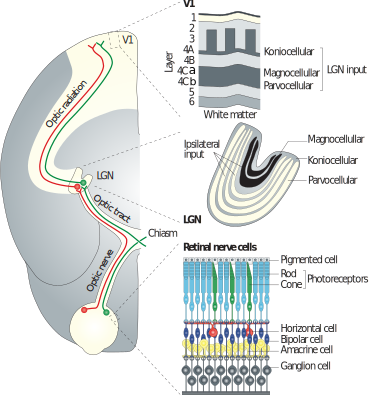
\includegraphics[width=0.6\textwidth]{./figures/basic_anatomy.pdf}
\caption{{\bf The mammalian early visual pathway.} Anatomy of the visual
  pathway from the photoreceptors in the retina through the lateral
  geniculate nucleus (LGN) in the thalamus to the primary visual cortex
  (V1). On the right, the anatomical structures at each stage of visual
  processing are shown. The top right schematic shows the photoreceptors
  at the back of the retina where light is transduced into an electrical
  signal which passes through the bipolar cells to the ganglion
  cells. The axons of the ganglion cells form the optic nerve which
  projects to the LGN shown in the middle schematic on the right. The
  LGN has a laminar arrangement where each layer aligns input from both
  eyes to form a retinotopic map of the contralateral portion of the
  visual field. The majority of the axons from LGN neurons then project
  via the optic radiations to V1, terminating in layer 4. The
  organization of the parvocellular, magnocellular, and koniocellular
  pathways is shown in both the LGN and V1 schematics, where the shading
  indicates the pattern that emerges when V1 slices are stained for
  the metabolic marker cytochrome oxidase. Reproduced from
  \citet{solomon_naturerev07}.}
\label{fig:basic_anatomy}
\end{figure}


The classical receptive field of a visually responsive cell corresponds
to the best stimulus pattern found to evoke a response. Figure
\ref{fig:example_RFs}A shows a schematic of the center-surround
receptive-field structure typical of a mammalian LGN ON cell as well as
an example recorded from cat. Part B of the figure shows the
corresponding schematic for a V1 neuron composed of an ON and OFF lobe
as well as a typical example of an oriented receptive field recorded
from simple cell in area 17 (cat). This elongated, Gabor-like receptive
field is also observed in macaque, as can be seen in the simple cell
spatiotemporal RF in Figure \ref{fig:example_RFs}C.

% jbednar: Maybe should use a directionally selective cell in C so that
% the spatiotemporal RF is more interesting?
\begin{figure}
\center
\includegraphics[width=0.9\textwidth]{./figures/example_RFs.pdf}
\caption{{\bf Example receptive fields in the LGN and V1.} (A) Schematic
  of a typical LGN center-surround receptive field next to an example
  recorded from an LGN ON cell. (B) Schematic of a typical V1 simple cell
  receptive field next to an example recorded from a V1 cell. The two
  examples are shown are recorded in cat and reproduced from
  \citet{deangelis_tin95}. (C) A spatiotemporal receptive field recorded
  from a macaque simple cell using subspace reverse correlation. The
  inset number shows the time in milliseconds at which the RF is
  computed. Reproduced from \citet{dario_jneurophys01}.}
\label{fig:example_RFs}
\end{figure}


The orientation-selective cells in V1 have a spatial
organization across the cortical surface that falls into two classes
when considering mammalian species. Rodents, for instance, have a ``salt
and pepper'' organization where orientations appear randomly distributed
down to the cellular level, as shown in Figure \ref{fig:example_OR_maps}A.
In contrast, carnivorans and primates such as macaque have a smooth orientation map
organization as seen in Figure \ref{fig:example_OR_maps}B and C. As the
model presented in this thesis aims to model the cortical response in
macaque, any orientation maps of the model should have this sort of
smooth organization.

\begin{figure}
\center
\includegraphics[width=0.9\textwidth]{./figures/rat_macaque_maps.pdf}
\caption{{\bf Example orientation maps in rat and macaque V1.}  (A)
  ``Salt and pepper'' arrangement of orientation preference in rat V1 as
  recorded with two-photon calcium imaging down to subcellular
  resolution. Preferences are indicated by the cyclic color key on the
  right. Reproduced from \citet{ohki_nature05}. (B) Orientation preference
  map recorded using optical imaging in anesthetized macaque using the
  same color key. The distance $\Lambda$ covers a change of $180^\circ$
  and corresponds to the hypercolumn distance. The white circles mark
  two pinwheel locations around which all preferences are
  represented. These two pinwheels have opposite polarities with a
  clockwise progression moving up the color key for the left pinwheel
  and a clockwise progression down the color key for the pinwheel on the
  right. (B) The corresponding orientation selectivity map. Reproduced
  from \citet{blasdel_jn92b}.}
\label{fig:example_OR_maps}
\end{figure}


Smooth orientation maps have more identifiable structure than salt and
pepper arrangements. In particular, as the map varies smoothly,
hypercolumns can be identified as a continuous region over which the
full set of receptive-field parameters are covered. In the case of
hypercolumns, this corresponds to the average distance over which the
orientation preference cycles over $180^\circ$. The corresponding
circular feature where a $180^\circ$ change in orientation preference is
observed around a point is called a pinwheel. Pinwheels have two
different polarities depending on whether the orientation preference
increases or decreases when circling the pinwheel center
clockwise. Examples of both these features are shown in Figure
\ref{fig:example_OR_maps}B. The orientation selectivity map is also
smoothly varying as shown in Figure \ref{fig:example_OR_maps}C.

In summary, the visual system is composed of a large population of
neurons with a diversity of receptive field and tuning properties. There
is organization that can be observed at the level of individual neurons
such as the receptive fields of a particular cell shown in Figure
\ref{fig:example_RFs} and there is organization that is only apparent
across a large population of cells, such as the orientation maps shown
in Figure \ref{fig:example_OR_maps}.

From this evidence, it is clear that there are different spatial scales relevant
to the visual response, ranging from single-unit recordings to
measurements of entire feature maps. In the next portion of this
chapter, the ways activity can be recorded across these different scales
will be discussed. This will included a common experimental approach for
measuring activity at the level of an individual neurons and then a
discussion of optical imaging techniques used to record from a large,
spatially extended population of neurons at once.


\section{Dynamics of the evoked response}
\label{section:evoked_background}

The first step toward validating a model of neural response in V1 is to
consider the available experimental data in the fully developed, adult
animal. In this section, the observed experimental responses to
artificial stimuli in adult macaque V1 are discussed, both at the level
of individual neurons and across a spatially extended population.

First the local spiking response will be considered in terms of the
peristimulus time histogram (PSTH) profiles of both simple and complex
cells in macaque. The experimentally observed PSTH profiles are
summarized by the invariant response descriptive model developed by
\citet{albrecht_jneurophys02}.

Next the evoked dynamics across a large population of neurons is
considered using voltage-sensitive--dye imaging, also recorded in
macaque. This technique captures the evoked pattern of response over
several square millimeters of the cortical surface with a high temporal
resolution. The key properties of the observed spatiotemporal dynamics
are then summarized as a function of stimulus contrast.

These two experimental techniques yield very different temporal profiles
for the evoked response. Understanding how these two sources of data can
be consistently accounted for within a single model of the evoked
response is the basis of Chapter \ref{chapter:SIRD}.

\subsection{Local spiking responses}

The temporal properties of the spiking response of a neuron can be
recorded using an electrode with a high temporal resolution, then
expressed as a peristimulus time histogram (PSTH). Such recordings
typically have a high enough temporal resolution to resolve individual
action potentials in a localized volume of neural tissue. One way to
begin quantifying the dynamics of the response of individual neurons in
the visual system is to examine the properties of PSTH profiles evoked
by an appropriate test stimulus. In this section, the PSTH profiles of
both LGN and V1 neurons will be presented.

\subsubsection*{Spiking profiles in the LGN}


The mechanistic models we will consider later on simulate the
propagation of activity from the photoreceptors in the retina to V1 via
the LGN. Therefore, in order to understand what drives the spiking
responses in V1 mechanistically, it is first useful to examine the
spiking response profiles in the LGN.

Figure \ref{fig:LGN_PSTH_maunsell} shows average PSTH profiles for
magnocellular and parvocellular neurons in macaque LGN. Both types of
cell have a peak in spiking activity although the ratio of the peak to
the sustained response is lower in magnocellular neurons. These PSTHS
have been plotted on a $150$ millisecond axis to allow easy comparison
with the V1 PSTH profiles described in the next section.

\begin{figure}
\center
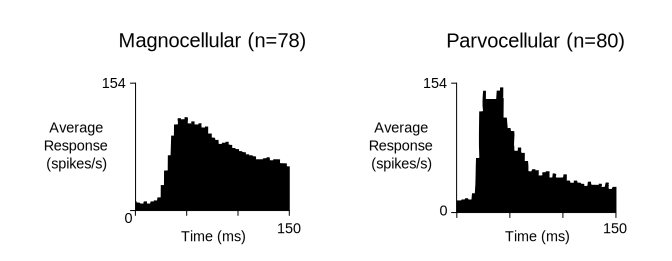
\includegraphics[width=0.9\textwidth]{./figures/LGN_PSTH_maunsell.pdf}
\caption{{\bf Average PSTH profiles for magnocellular and parvocellular
    LGN neurons in anesthetized macaque.} Cells were stimulated by
  $0.25^\circ$ radius spots that were either brighter (ON) or darker
  (OFF) than the background by $28$ \si{cd/mm^{2}}.  On the left, the
  average PSTH profile for 78 magnocellular neurons is shown. On the
  right, the average PSTH for 80 parvocellular neurons.  Data reproduced
  from \citet{maunsell_visneuro99}.}
\label{fig:LGN_PSTH_maunsell}
\end{figure}


\subsubsection*{The invariant response descriptive model}
\label{section:IRD_background}

The invariant response descriptive (IRD) model of
\citet{albrecht_jneurophys02} offers a mathematical description of the
experimentally observed spiking response of V1 cells. This
phenomenological model summarizes the observed PSTH profiles as a
function of stimulus contrast for simple and complex cells of adult cat
and monkey. For a population of 50 cells, this model was found to
account for approximately 94\% of the variance observed across the
microelectrode recordings and will serve as a way to quantify the
properties of ``typical'' PSTH profiles.

The temporal spiking response profiles of cortical neurons vary in both
shape and amplitude according to the particular cell that is being
recorded, as well as the shape of the driving stimulus. It is nonetheless
useful to try to capture the general properties of observed PSTH
profiles with a simple descriptive model.

The invariant response descriptive (IRD) model is a phenomenological model
that captures the shape of a typical PSTH profiles over 200 milliseconds
in response to the presentation of a stationary sinusoidal grating
pattern at a fixed contrast. First, the profile shape is approximated in
a piecewise manner using a Gaussian function up to the peak value at
$\tau_c$ and a ``$\frac{1}{2}$ Gaussian'' profile to capture the
sustained response thereafter:
%%
\begin{equation}
\label{eq:IRD_half_gaussians}
r_t(t) =
\begin{cases}
 \exp \left( -\ln 2 \frac{(t - \tau_c(c))^2)}{\sigma^2_a} \right) & t < \tau_c \\
      \exp \left( -\ln 2 \frac{(t - \tau_c(c))^2)}{\sigma^2_b} \right) + (1 - \alpha) \exp \left( -\ln 2 \frac{(t - \tau_b(c))^2)}{\sigma^2_c} \right) & t\geq \tau_c
   \end{cases}
\end{equation}
%%
The time to the peak response $\tau_c$ is described with a
contrast-dependent offset computed according to an inverted Naka-Rushton
equation.  The relative response amplitude $r_c(c)$ is defined in a
similar way:
%%
\begin{equation}
\label{eq:IRD_latency}
\tau_c(c) = \tau_{max} - \tau_{shift} \frac{c^\epsilon}{c^\epsilon + s_{50}^\epsilon}
\end{equation}
%%
\begin{equation}
\label{eq:IRD_amplitude}
r_c(c) =\frac{c^n}{c^n + c^n_{50}}
\end{equation}
%%
The PSTH profiles are then described as the product of these terms
offset by a fixed response $r(t,c) = r_{max} r_c(c)r_t(t) + r_0$ where
$r_{max}$ is used to scale all the responses by a constant factor.

The mean parameter values, the bounds at one standard deviation and the
corresponding median values given in \citet{albrecht_jneurophys02} are as
follows: $\sigma_a = 19.0 \pm 1.9.1, 13.6; \sigma_b = 761 \pm 76.5, 543;
\alpha=0.27 \pm 0.03, 0.23; n = 2.5 \pm 0.18, 2.2; c_{50}=38.7 \pm 3.51,
32.3; \tau_{max} = 121 \pm 4.53, 114; \tau_{shift}=65.3 \pm 3.48, 61.2;
\epsilon=1.80 \pm 0.28, 1.18; s_{50}=24.6 \pm 3.27, 23.1; r_{max}=81.8
\pm 12.2, 50.9$. Note that the median is outside of one standard
deviation from the mean for nearly all of these parameters.

Taking the median values for these constants, we can use this model to
generate a set of temporal response profiles as a function of contrast
as shown in Figure \ref{fig:IRDModel}. As expected, there is an onset
peak that occurs before the first hundred milliseconds at high contrast,
followed by a sustained response. Note that this model only captures the
onset response when the stimulus is turned on, and does not capture how
the response decays once the stimulus is turned off.

\begin{figure}
\center
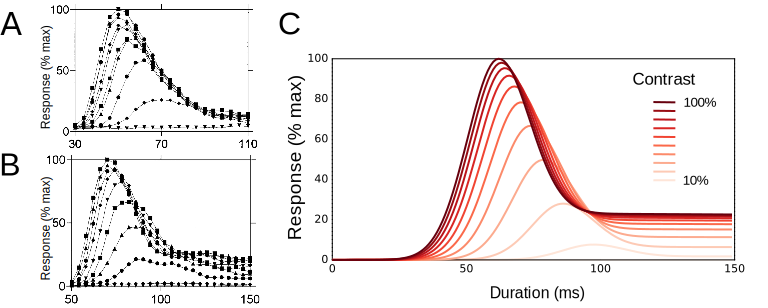
\includegraphics[width=0.8\textwidth]{./figures/IRD_example.pdf}
\caption{{\bf Behavior of the invariant response descriptive model for
    ten different contrasts}. Each plot starts at 10\% contrast and ends
  at 100\% contrast in steps of $10\%$.  (A) Example PSTH record from a
  macaque simple V1 cell across all ten contrasts where all PSTHs are onset
  aligned. (B) Similarly aligned example PSTHs recorded from a macaque
  V1 complex cell. (C) Output of the IRD model, replicated using the
  published median parameter values. Experimental data reproduced from
  \citet{albrecht_jneurophys02}.}
\label{fig:IRDModel}
\end{figure}

This concludes the background material regarding single-unit activity
recording, as the IRD model is a sufficiently detailed level of
description for the firing-rate models presented in this thesis. Next we
turn to an experimental technique used to record activity from entire
populations at once.


\subsection{Voltage-sensitive--dye imaging} % do hyphenate!
\label{section:VSDI_background}

Voltage-sensitive--dye imaging (VSDI) is an optical imaging technique
that measures the neural activity over a large cortical area with a high
temporal resolution. Unlike the intrinsic optical techniques suitable
for chronic studies such as those described in section
\ref{section:ferret_map_stability}, voltage-sensitive--dye imaging
requires the direct application of a dye to the cortical surface.

The voltage-sensitive dye binds to the external surface of all the cell
membranes it comes into contact with (including both neurons and glial
cells), acting as a transducer from
electrical potential to optical signal. The dye responds rapidly to
changes in the local voltage, giving the technique sub-millisecond
resolution over several millimeters squared of cortex. A good
review of the technique may be found in 
\citet{grinvald_natneuro05} and \citet{chemla_jphys10}.

The optical signal indicates the voltage
change across the whole tissue, as a mixture of both subthreshold and spiking
response. As the dye seeps into the neural tissue from the cortical
surface, there is a depth-dependent fluorescence gradient, with little dye
binding at depths greater than 800 \si\micro m.  The charge-coupled
device (CCD) records the photonic flux from above the cortical surface,
which results in a signal that is biased towards activity in superficial
layers.

The spatial resolution of a typical frame output by the CCD is around
20\si\micro m -- 50\si\micro m per pixel, where each pixel is integrating
the photonic emission from a small cortical volume. The scale of
scattering of photons in the neural tissue is approximately 200
\si\micro m \citep{orbach_jn83} which determines the primary limiting
factor in the spatial resolution of the technique.

These features of VSDI make it an excellent way to record the evoked
activity dynamics of a large cortical population. The indiscriminate
binding of the dye to all available cell membrane allows recording of
the bulk electrical response, but it also complicates the process of tracing
the exact contributions of different neural populations to the overall
signal.


\subsubsection*{Spatiotemporal dynamics of the VSDI response}
\label{section:VSDI_dynamics_background}

A preliminary step towards understanding the spatiotemporal dynamics
observed with VSDI is to observe the evoked activity in response to a
simple stimulus that is flashed on and off. A simple stimulus protocol
helps reveal the basic properties of the VSDI signal in the absence of
complicating factors such as varying stimulus motion or shape. Even
using the simplest possible flashed stimuli, the observed spatiotemporal
dynamics will still depend on factors such as the stimulus size,
retinotopic location, the spatial profile of the stimulus, the duration of
presentation and the stimulus contrast.

Two different sources of experimental data obtained from two different
laboratories will help reveal the general properties of the VSDI
response in macaque V1 \citep{sit_neuron09,reynaud_jn12}. Both of these
sources of data will help constrain the spatial model of population
response presented in Chapter \ref{chapter:SIRD}.

\paragraph*{\citet{sit_neuron09}}

%%  Trials lasted 999 ms, with a 100 ms delay, 600 ms visual
%% stimulation, and poststimulus delay of 299 ms. We typically recorded
%% 60 trials per condition. Visual stimuli were drifting sinusoidal
%% gratings of different contrasts.

The VSDI data published in \citet{sit_neuron09} is summarized in Figure
\ref{fig:sit_data}, showing the response evoked by a flashed Gabor
stimulus in awake, fixating macaque. A $0.167^\circ$ Gabor stimulus at
$2.2^\circ$ eccentricity was turned on at time zero and sustained for 200
milliseconds with the VSDI response recorded over a period of 500
milliseconds. The spatial profile of the VSD signal at the time of peak
response was found to be approximately Gaussian as shown in Figure
\ref{fig:sit_data}A--C. Six different contrast levels were used with
subfigures A and B of Figure \ref{fig:sit_data} showing the peak spatial
response evoked by $6\%$ and $100\%$ contrast Gabors respectively.

\begin{figure}
\center
\includegraphics[width=0.95\textwidth]{./figures/sit_data.pdf}
\caption{{\bf Dynamics of the VSDI response in macaque V1 observed in
    \citet{sit_neuron09}}. Response evoked by a $0.167^\circ$ Gabor
  stimulus flashed on from time 0 to 200 ms. (A) Example peak response
  for stimulus at $6\%$ contrast. Color bar indicates normalized
  response and scale bar marks a distance of 3mm across the cortex. (B)
  Example response at $100\%$ contrast. (C) Layout of spatial regions of
  interest (ROIs) shown on top of a Gaussian fit of the response in
  (B). The strip is 1mm wide and each circular annulus has a width of
  0.5 mm. (D) Plots of the spatiotemporal response averaged in the ROIs
  shown in (C). Each plot is the spatiotemporal response at the
  indicated stimulus contrast with each plot composed of a horizontal
  strip per ROI at the indicated position. Each strip is a 500
  millisecond long fit of the mean response in the ROI to a logistic
  function based on the response at $10\%$, $50\%$, and $90\%$ of the
  maximum. Each row in such a strip is normalized independently,
  and then displayed according to the color bar on the left.}
  \label{fig:sit_data}
\end{figure}

The annular regions of interest (ROIs) used in the spatiotemporal
analysis are shown in subfigure C. The central region is circular, with
all remaining ROIs constructed by intersecting a millimeter-wide strip
with nested concentric rings, each ring incrementing the radius by $0.5$
millimeters. In Figure \ref{fig:sit_data}D, the average responses in the
six ROIs are presented for the whole 500 millisecond period across all
six different stimulus contrasts. The average response of each ROI is
shown as a thin strip, with the mean central circular ROI response shown
and the mean response of the most distal annulus shown at the bottom.

The spatiotemporal plots shown in Figure \ref{fig:sit_data}D are a
useful way to summarize the response dynamics over time and space and
will be used extensively in Chapter \ref{chapter:SIRD}. For reasons that
will be discussed later, only the onset portion of the responses up to
$200$ ms will be examined. There are several features of interest in the
onset response: (1) the initial onsets are nearly vertical in the
spatiotemporal plots, suggesting the initial response appears at roughly
the same time across cortical space, (2) towards the peak of the
response, a spatiotemporal gradient develops with more distal regions
responding more slowly, and (3) as overall stimulus contrast decreases, the
overall latency of the responses increases.

All these properties are inferred from the six plots shown in
Figure \ref{fig:sit_data}. It is important to understand that these
plots could potentially be misleading as they do \emph{not} show the
experimental data directly. Instead, what is actually shown in each row
is a piecewise-fit to a rising and falling logistic function. These
logistics are constrained using the response at $10\%$, $50\%$, and
$90\%$ of the maximum amplitude.

This means the responses are always going to be smooth within each ROI
as the logistic function that is representing the data is smooth. If the
fitting error is high, it is conceivable that the true VSD signal has a
very different profile that is obscured by this fitting procedure. For
this reason, we need to verify that the raw VSD signal does rise slowly
and plateau, in order to ensure the logistic fit is not invalid.

\paragraph*{\citet{reynaud_jn12}}

It is worth considering a second source of experimental data to ensure
that the plots in Figure \ref{fig:sit_data} are a suitable summary of
the VSD response after the application of the logistic fits. This is
achieved by Figure \ref{fig:reynaud_data} which shows the raw $\Delta
F/F$ responses from \citet{reynaud_jn12} visualized using the same
format of spatiotemporal plot.

Each such plot shows the response averaged in the three ROIs shown in
Figure \ref{fig:reynaud_data}A using the same color map as Figure
\ref{fig:sit_data}D. Although the shape and position of the ROIs are not
the same as those used in \citet{sit_neuron09}, the general properties
of the raw VSD signal across space and time remain consistent.

\begin{figure}
\center
\includegraphics[width=0.95\textwidth]{./figures/reynaud_data.pdf}
\caption{{\bf Dynamics of the VSDI response in macaque V1 observed in
    \citet{reynaud_jn12}}. (A) Left, ocular dominance map used to delimit
  the boundary between V1 and V2. Right, image of the cortical
  vasculature annotated with the three labeled regions of interest used
  in analysis. White dotted arcs indicate retinotopic representations of
  the stimulus for the center (2$^\circ$ diameter) to the periphery
  (dotted arc-circles at 1$^\circ$ and 1.8$^\circ$ eccentricity to the
  center outer border). (B) Example of the $\Delta F/F$ VSDI response
  over time for the $60\%$ contrast stimulus. Stimulus consists of a
  drifting sinusoidal gratings presented behind a circular window
  (2$^\circ$ diameter) (C) Spatiotemporal plots of the $\Delta F/F$
  response for four different stimulus contrasts plotted in the format
  used by \citet{sit_neuron09}.}
  \label{fig:reynaud_data}
\end{figure}


Generalizing the experimental results from both studies, it is clear
that the dynamics of the VSDI response is qualitatively very different
from the PSTHs of the spiking response shown in Figure
\ref{fig:IRDModel}. In the $200$ millisecond period in which the Gabor
is presented, the VSD signal slowly reaches a plateau, whereas the PSTHs
expressed by the IRD model are long past their peak. Because of this large
discrepancy between PSTH and VSDI profiles, it has been difficult to
interpret findings from VSDI, and so it is important to resolve these
conflicting views of temporal evoked responses.  Achieving such
a resolution is the topic of Chapter
\ref{chapter:SIRD}.

\section{Development of feature selectivity}
\label{section:development_background}

In the experiments described in the previous section, oriented stimuli
were used to evoke a neural response, because the neurons of the primary
visual cortex are driven strongly by oriented visual stimuli. In adult
macaque V1, strong orientation selectivity is expected assuming the
animal has reached visual maturity. In order to account how neurons
become feature selective in the first place, it is necessary to
understand how the cortical response changes over the course of visual
development.

Observing the neural response over development requires difficult and
time-con\-suming chronic experiments. First, the animals need to undergo
experimental preparation involving surgery. After surgery, every
precaution must be taken to ensure the animal makes a full recovery in
order to avoid later complications. The experimenter has to be
constantly available for several weeks, in order to perform regular
recordings and to ensure that both the animal and the experimental
preparation is kept stable. Single-unit studies are particularly
difficult, as keeping track of an individual neuron over many weeks
with an electrode preparation is nearly impossible.

These practical difficulties make chronic studies a risky proposition
for an experimenter, involving a high investment of time and laboratory
resources for uncertain gains. When acute studies can yield useful
scientific results far more quickly, it is not surprising to discover
that there are far fewer chronic studies published in the literature.
%%
Specifically, there is essentially no published data that tracks how
individual V1 neurons respond over development, in a mammalian species
with smooth maps.  Two-photon imaging techniques may soon make this
sort of recording possible, but so far none have been published.
% Fitzpatrick lab showed some at SfN 2014; doesn't
% seem to be published yet.

\subsection{Robust and stable orientation map development}
\label{section:ferret_map_stability}

Luckily, at the population level, chronic optical imaging data of
orientation map formation is available, though only for ferret V1
\citep{chapman_jn96}.  The properties of orientation maps as they
emerge in a maturing animal are an important constraint on any
developmental model simulating a large region of V1, and so this data
is a crucial point of reference despite potential species differences.
This study of eight ferret pups also gives some insight into how the
average orientation selectivity changes over development, as
(non-chronic) electrode recordings were carried out over similar time
periods.

Figure \ref{fig:ferret_stability} shows the development of the
orientation map preference and selectivity in a single animal from
postnatal day 31 to postnatal day 42. As orientation selectivity
increases, the map structure gradually becomes apparent without a
significant rearrangement in the spatial arrangement over time from p33
onwards. In other words, the neurons become more selective over
development but the orientation map structure itself is stable.


\begin{figure}
\center
\includegraphics[width=1.0\textwidth]{./figures/ferret_stability.pdf}
\caption{{\bf Stable development of orientation maps in ferret striate
    cortex}. Maps shown were recorded from a single animal, reproduced
  from \citet{chapman_jn96}. Each pixel shows the orientation preference
  according to the key above and pixel value indicates the
  orientation selectivity, with black indicating relatively
  unselective regions. Each map has the selectivity scale normalized
  independently, revealing blood vessels at P31 even though these
  features have no significant orientation selectivity. As the map
  matures, the stability of the spatial structure of the map is apparent,
  as selectivity increases but the overall map pattern stays constant.}
  \label{fig:ferret_stability}
\end{figure}


In \citet{chapman_jn96}, the stability of orientation maps recorded with
intrinsic optical imaging is evaluated over development using a map
similarity metric. This similarity is calculated as the maximum mean
orientation difference between the map measured on a particular
postnatal day with the final map recording. Dividing these mean
difference values by 90 and subtracting the result from one yields a
normalized index that varies between zero and one. A value of zero
indicates anticorrelation, a value of a half indicates no correlation,
and a value of unity indicates identical maps.

Using this similarity metric as well as a selectivity measure obtained
from the optical signal, it is shown that orientation selectivity
continues increasing well after the maps have attained a stable
spatial organization early on in development. These results are shown in
Figure \ref{fig:chapman_data}.

In order to validate the selectivity measure obtained from the optical
signal, additional recordings were obtained over development using
single-cell electrophysiology. It was found that these more traditional
measurements of orientation selectivity correlated well with the
orientation tuning measured with optical imaging. As a result, we can be
confident that the observed selectivity changes in the orientation maps
are also reflected at the level of individual neurons.

\begin{figure}
\center
\includegraphics[width=1.0\textwidth]{./figures/chapman_data.pdf}
\caption{{\bf Selectivity and stability of ferret orientation maps over
    development.} (A) Change in orientation selectivity over
  development, plotting orientation tuning index against postnatal age
  in days. Points indicate tuning index values recorded with single-cell
  electrophysiology and the solid line shows the corresponding sigmoid
  fit. The dashed lines shows the sigmoid fit based on the optical
  imaging data. (B) The orientation similarity index of the recorded
  maps for eight ferrets for experimental (filled squares) and control
  conditions (open squares). The difference between these conditions is
  that the controls use between-animal comparisons of similarity whereas
  the experimental condition shows the similarity of the recorded map
  with the final map measurement within the same animal. Reproduced from
  \citet{chapman_jn96}.}
\label{fig:chapman_data}
\end{figure}

Taken together, Figures \ref{fig:ferret_stability} and
\ref{fig:chapman_data} show that map development exhibits
\emph{stability} while developing \emph{selectivity}, but
there is one other property that will be important in the analysis
presented in Chapter \ref{chapter:GCAL}. Orientation map development is
also \emph{robust} against differences in inputs, as similar final map
patterns develop until nearly 3 weeks of age in cats, regardless of
whether the eyes are open \citep{crair_science98}. Development of
selective orientation maps therefore appears to be both robust and
stable.

%% If I were to included the Tanaka data, it would go here...

What this section has showed is that there is emergent structure at the
population level in terms of how the feature preferences of neurons are
organized over cortical space. The smooth organization of orientation
maps demonstrates that neurons do not develop their receptive fields
independently from one another with local regions of cortex having
neurons with similar preferences. In order to understanding this
process, it is necessary to put these experimental results into a
theoretical framework.

In the next section, one type of modeling approach that can account for
feature map formation over development will be introduced. A particular
self-organizing map model will be described that accounts for the stable
and robust orientation map development shown in Figure
\ref{fig:chapman_data}. This model will be the basis of the work done in
Chapters \ref{chapter:GCAL} and \ref{chapter:TCAL} of this thesis.


\section{Self-organizing network models}
\label{section:self_organizing_networks}

Self-organizing map models attempt to explain the emergence of feature
selectivity and smooth feature maps through the repeated operation of
simple, preferably local learning rules for modifying synaptic
strengths and other properties of simulated neurons.  The models
are driven by afferent input from outside the cortical region, and
typically achieve organization through ``lateral'' interactions
between neurons in a region, across the cortical surface.

The fundamental behavior of self-organizing network models, as
introduced by \citet{malsburg_kyber73}, is to establish a topological
mapping from a high dimensional feature space of the visual input onto a
two dimensional cortical surface. The ability to preserve continuity of
the input space using unsupervised learning is also used as a general
data visualization and analysis in the well known Kohonen
self-organizing map model (SOM) \citep{kohonen_biocyber82}.

The core principle used to update the synaptic strengths in these
networks is Hebbian learning \citep{hebb_book49}. In brief, when the
pre- and postsynaptic activity is relatively high, the corresponding
synaptic weights increase. This most basic rule would result in
monotonically increasing synaptic weights, and so there also needs
to be a mechanism to decrease synaptic strength. The mathematical
formulation of one such rule, divisive postsynaptic weight
normalization, will be described shortly for a particular
self-organizing map model.

When trained with visual patterns, self-organizing model units can develop
orientation selectivity and self-organize spatially in a way that
appears very similar to the smooth maps that are experimentally
observed. This observation has inspired a number of different developmental
models of feature map formation based on the principles of
self-organizing maps \citep{obermayer_pnas90,miikkulainen_2005}.

All models related to the SOM rely on lateral interactions to preserve
the topological representation of the input feature space when the model
weights are updated. Depending on the training stimuli and model
architecture, other maps such as direction, disparity, and spatial
frequency maps can be simulated and even combined within a single model
\citep{miikkulainen_2005,bednar_jpp12}. One fundamental mathematical
principle underpinning these models can be expressed as
dimensionality reduction, and some forms of the model have been shown
to be equivalent to discretized approximation of the principal
surfaces of the input distribution \citep{ritter_92}.

In the next section, a particular example of a self-organizing map model
called GCAL will be defined, as this model is the basis of much of the
work in this thesis. One the architecture and core equations of GCAL are
defined, it will be used to illustrate the fundamental principles of
self-organization and development in this class of model.

\subsection{The GCAL model}
\label{section:GCAL_background}

The GCAL (gain control, adaptation, and lateral) model is the
successor to the LISSOM model \citep{miikkulainen_2005}, replacing it for all current
purposes. GCAL was developed originally by Judith Law, Jan Antolik,
and James A.\ Bednar, but it was first published in
\citet{stevens_jn13} only after I added the systematic analyses
outlined in chapter \ref{chapter:GCAL} that demonstrate that it
robustly and stably achieves high selectivity and realistic maps.

Compared to LISSOM and other related models, GCAL is simpler, more
biologically plausible, and yet 
more robust in its ability to form high-quality orientation maps. The
statistics of GCAL orientation maps are analyzed in Chapter
\ref{chapter:GCAL} to quantify their match to biological results
across training conditions, and this model is the basis of the new
developmental models presented in Chapter \ref{chapter:TCAL}.

Like LISSOM, the GCAL model is driven by input patterns that correspond
to visual images, patterns of spontaneous activity, or measurement
conditions during model training and measurement. Each input pattern is
represented as a two dimensional array of activations at the
photoreceptor sheet, which then drives the activity of neural sheets
later in the visual pathway. Each sheet is a two-dimensional array of
computational units where each unit has a scalar activity value.
Sheets are connected together by projections where a projection between two
sheets specifies the weight contributed by the input sheet, for every
unit of the output sheet.

During training, an incremental Hebbian learning rule is applied to all
plastic projections once the network dynamics have settled towards a steady state in the cortical
sheet in response to each individual training pattern presented to the
network. The cortical sheet is driven by afferent projections from
separate ON/OFF sheets that serve to model the ON and OFF receptive
fields of RGC/LGN cells. The architectural schematic of the GCAL model
is shown in Figure \ref{fig:GCAL_schematic}.

\begin{figure}
\center
\includegraphics[width=0.6\textwidth]{./figures/GCAL_schematic.pdf}
\caption{{\bf Architecture of the GCAL model.} Connections to the central unit
  in each sheet are shown with afferent connections in yellow and
  lateral connections in red. In the cortical sheet, there are two types of lateral connections with different spatial profiles. The short range connections are excitatory and the longer range connections are inhibitory.}
  \label{fig:GCAL_schematic}
\end{figure}

GCAL is governed by two core equations.  The first specifies how the
activity is computed at each unit of each sheet. The second specifies
the learning step
that adjusts the weights of the plastic projections once activity has
settled in the network. The rest of the model is specified in terms of
the initial weight patterns, the statistics of the training inputs, and
the transfer functions that map the input activity per unit into an
output activity (which corresponds to the spike rate).


\subsubsection*{Activity integration per unit}

The activity at each unit at a given simulation timestep is found by
summing the activity contribution $C_{j,p}$ of projection $p$ over all
the projections feeding into the unit $j$. Each contribution is computed
by treating the incoming weight as a vector and taking the dot product
of this weight vector $\omega$ with the corresponding activations
$\eta_{i,p}$ from the source sheet in the connection field $F_{j,p}$.
%%
\begin{equation}
  \label{eq:projection_activity}
C_{j,p}(t+\delta t) = \sum_{i \in F_{j,p}} \eta_{i,p}(t) \omega_{ij,p}
\end{equation}
%%
One feature GCAL introduces that is not present in the earlier LISSOM model is a
contrast-gain control mechanism in the ON/OFF sheets. This is
implemented using lateral divisive inhibitory projections in the ON and
OFF sheets. Contrast-gain control is a well established phenomenon (see
\citealt{carandini_nature12} for a review) and was found to improve the
robustness of map formation in the GCAL model in a way that is
rigorously quantified in Chapter \ref{chapter:GCAL}.

Combining the afferent and contrast-gain control contributions allows
the output activity of the ON or OFF sheets $O$ to be described with the
following equation:
%%
\begin{equation}
  \label{eq:ON_OFF_activity}
  \eta_{j,O} (t + \delta t) = f \left(
  \frac{\gamma_O \sum_{i \in F_{j,P}} \Psi_i (t) \omega_{ij}}
       {k + \gamma_S \sum_{i \in F_{j,S}} \eta_{i,O} (t) \omega_{ij,S}} \right)
\end{equation}
%%
The numerator corresponds to the contribution as specified in Equation
\ref{eq:projection_activity} for photoreceptor activities $\Psi_i$ weighed
by the overall afferent projection strength $\gamma_O$. The $\gamma_S$
constant is the strength of the inhibitory gain control projection
expressed in the denominator. The constant offset $k$ is necessary to
ensure activity is defined for weak inputs. $f$ is a half-wave
rectifying function.

In the cortical layer, the contributions specified by Equation
\ref{eq:projection_activity} are summed over the ON, OFF, lateral
excitatory, and lateral inhibitory projections, where the lateral
inhibitory component is negative to model a subtractive effect of
relatively long-range
inhibition (up to a couple of millimeters of cortical tissue). The
total of these contributions is passed through the 
transfer function specified in Equation \ref{eq:adaptation} and the
network is allowed to settle for 16 timesteps to allow the network activity to settle, before the Hebbian learning rule given in Equation
\ref{eq:hebbian_learning} is applied.

\subsubsection*{Weight profiles of the initial condition}

The weight profiles for the afferent and lateral projections in the
ON/OFF sheets are static. The weight $\omega_{ij}$ from photoreceptor
$i$ to the ON or OFF unit $j$ is defined by a standard difference-of-
Gaussians profile to model LGN receptive fields:
%%
\begin{equation}
\label{eq:ON_OFF_DoG}
\omega_{ij} = \frac{1}{Z_C} \exp \left( \frac{x^2 + y^2}{2 \sigma^2_C}\right)
   - \frac{1}{Z_S} \exp \left(\frac{x^2 + y^2}{2 \sigma^2_S} \right)
\end{equation}
%%
Here the $x$ and $y$ values are the spatial position of the unit
relative to the central location $(0,0)$, the central $C$ and surround
$S$ Gaussian sizes are specified by $\sigma_C$ and $\sigma_S$
respectively and $Z_C$ and $Z_S$ are normalization constants that ensure
each term sums to 1.0. The OFF weights are simply the negation of the ON
weights given in Equation \ref{eq:ON_OFF_DoG}.  The size of the
center and surround is given by $\sigma_C=0.037$ and $\sigma_S=0.15$
respectively.

The static weights of the lateral inhibitory gain control projection in
the ON/OFF sheets are specified using a straightforward Gaussian profile
where the equation is generalized for any projection $p$:
%%
\begin{equation}
\label{eq:GC_Gaussian_Weights}
\omega_{ij,S} = \frac{1}{Z_p} \exp \left( -\frac{x^2 + y^2}{2 \sigma_p^2}\right)
\end{equation}
%%
The $x$ and $y$ values specify the location of the presynaptic neuron
and $Z_P$ is the normalizing factor that ensures that the total lateral
inhibitory weight sums to 1.0 for each unit. The size
of this spatial normalization pooling $S$ is given by the above equation
where $\sigma_S=0.125$ and $p=S$.

The weight of the lateral excitatory connection $E$ is also described
by Equation \ref{eq:GC_Gaussian_Weights} using $\sigma_E=0.27$ and
$p=E$. The weights for the afferent weights of the V1 sheet and the
lateral inhibitory projection are not pure Gaussians but consist of
samples from a uniform random distribution multiplied by a Gaussian
envelope described by Equation \ref{eq:GC_Gaussian_Weights}. For the
afferent weights (A) the envelope has $\sigma_A=0.27$ and for the
lateral inhibitory projection (I) the weight envelope has
$\sigma_I=0.075$. Note that for the purposes of computing the
normalization factor $Z_p$, the weights for each projection are defined
within a circle of radii $r_A=0.27, r_E=0.1$, and $r_I =0.23$.

\subsubsection*{Homeostatic threshold adaptation}

The transfer function used in the ON/OFF sheets has already been
described as simple half-wave rectification ($f$ in Equation
\ref{eq:ON_OFF_activity}). Computing the final activity of the cortical
sheet is more complicated, because an adaptive per-unit threshold is employed
in GCAL. This transfer function corresponds to a homeostatic threshold
adaptation mechanism that is found to improve the map quality of the
GCAL model in a way that is rigorously quantified in Chapter
\ref{chapter:GCAL}.

This adaptive threshold adjusts in response to the smoothed exponential
average of the settled activity $\bar{\eta}_j$ with smoothing parameter
$\beta$:
%%
\begin{equation}
  \label{eq:exponential_avg}
  \bar{\eta}_j(t) = (1 - \beta) \eta_j (t) + \beta \bar{\eta}_j (t - 1)
\end{equation}
%%
This exponential average is then used to compute the threshold $\theta$
at time $t$ using homeostatic learning rate $\lambda$ and target average
$\mu$:
%%
\begin{equation}
  \label{eq:adaptation}
  \theta (t) = \theta (t - 1) + \lambda ( \bar{\eta}_j (t) - \mu)
\end{equation}
%%
The value of smoothing parameter in GCAL is given by $\beta=0.991$, the
learning rate is given by $\lambda=0.01$, and the average target
activity per unit is specified by $\mu=0.024$, which also sets the
initial value of $\bar{\eta}_{jA}(0)$.

\subsubsection*{Normalized Hebbian learning}

Now that the means to compute all the activities of the units in the
network has been defined, the last step is to specify the learning rule
used to update the projection weights. On the first iteration of the
model, the weights have the initial distributions specified in the
equations above. Then with a timestep of $t=0.05$, activity propagates
through the network with connection delays that also have a value of
$t=0.05$. Activity from the ON/OFF sheets are only propagated after
contrast-gain control has been applied and then 16 simulation steps are
executed to allow the activity to settle in the cortical layer. At
this point, normalized Hebbian learning is applied before all activity
is cleared and the network is presented with the next training stimulus.

In GCAL, only the afferent weights feeding into the cortical layer and
the long-range lateral inhibitory weights are plastic. The
weights to the ON/OFF sheets are static, to focus on development at
the cortical level.  The short-range lateral weights in the cortical
sheet are also static, as plasticity in these lateral excitatory
connections has been found to have little effect.

Once the activity has
settled at the end of a training presentation, all the plastic
connections are adjusted using a simple, normalized model of
activity-dependent plasticity:
%%
\begin{equation}
  \label{eq:hebbian_learning}
  \omega_{ij,p}(t) = \frac{\omega_{ij,p}(t-1) + \alpha \eta_j\eta_i}
        {\sum_k (\omega_{kj,p} (t - 1) + \alpha \eta_j \eta_k )}
\end{equation}
%%
This equation expresses Hebbian learning that specifies how a synaptic
weight changes for a given learning rate $\alpha$ and pre- and
postsynaptic activities of $\eta_i$ and $\eta_j$ respectively. The
denominator applies divisive postsynaptic weight normalization to
prevent runaway increases in strength, which models another form of
homeostatic adaptation.

\subsection{Principles of self-organization}
\label{section:self_organization_principles}

Now that the GCAL model has been formally defined, it can be used to
illustrate the principles of developmental self-organization in this
class of model. This will make sense of the model structure and help
develop an intuition for the equations involved. When it comes to
understand self-organization, it is Equation
\ref{eq:GC_Gaussian_Weights} that is critical as it defines the shape of
the lateral weight profiles in the cortical sheet. Lateral interactions
are what drive the self-organization process, not only in GCAL but in
earlier map models, such as the more abstract Kohonen self-organizing
map model.

In the Kohonen self-organizing map model, the lateral interactions
necessary for smooth map formation are computed by locating the
maximally responding unit in the cortical sheet and imposing a spatial
Gaussian kernel at that location in the learning step
\citep{kohonen_biocyber82}. Such an operation requires a biologically
implausible global supervisor, a requirement that is removed in later
models such as the LISSOM (Laterally Interconnected Synergetically
Self-Organizing Map) model
\citep{sirosh_biocyber94,miikkulainen_2005}. The spatial profile of
Hebbian learning in the cortical sheet is fundamental to the
self-organization process, and in LISSOM, the necessary lateral dynamics
are modeled with explicit excitatory and inhibitory lateral
connectivity.

The GCAL model has the same effective Mexican-hat inhibition profile
introduced by LISSOM, shown in Figure \ref{fig:Mexican_hat} that drives
smooth map formation and is implemented with short-range excitatory
connectivity and long-range inhibitory connectivity. This organization
specifies the \emph{effective} lateral dynamics as a function of
distance across the cortex, even though cortical anatomy suggests the
inverse arrangement. What is important about Equation
\ref{eq:GC_Gaussian_Weights} is that the spatial extents of the
excitatory lateral connections are smaller than those of the inhibitory
connections.

Related but more detailed self-organizing map models such as LESI 
\citep{law_thesis09} and LESPI \citep{rudiger_thesis16}
show how it is possible to achieve the necessary
effective Mexican-hat profile while retaining anatomically plausible
connectivity of relatively short-range inhibition and longer range
excitation. Whether such an account is actually necessary to explain the
dynamics of self-organization is debatable as large, inhibitory basket
cells exist in the cortex that span at least one orientation hypercolumn
\citep{buzas_compneurol02}. As a result, the anatomical basis for
Mexican-hat interactions are not entirely clear \citep{kang_pnas02} and
for this thesis we will retain the Mexican-hat organization for
simplicity and ease of implementation.

\begin{figure}
\center
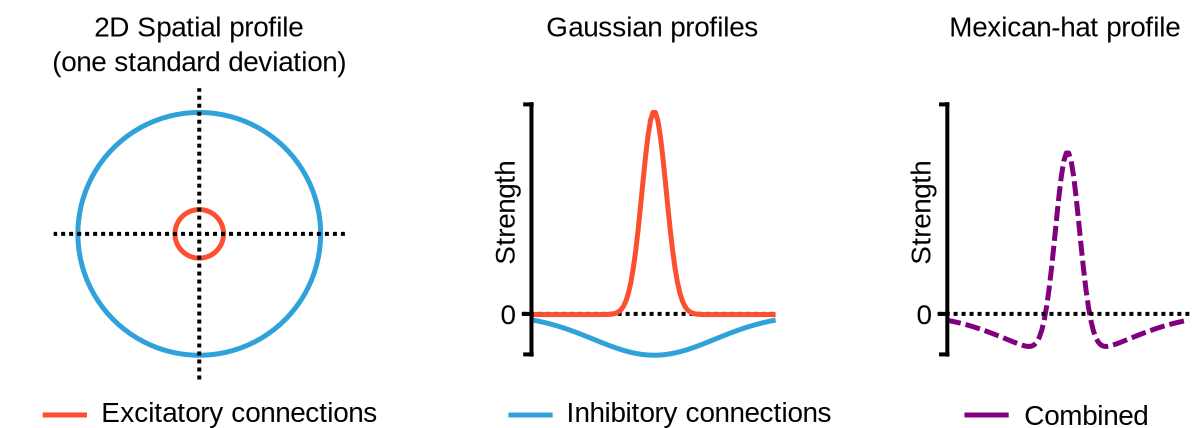
\includegraphics[width=0.9\textwidth]{./figures/Mexican_hat.pdf}
\caption{{\bf Schematic of Mexican-hat inhibition profile that drives
    activity bubble formation necessary for smooth map organization, as
    implemented by two types of connection.} (A) Schematic view of the
  cortical surface with one unit (center of the cross) making both short
  range excitatory lateral connections (red) and longer range inhibitory
  connection (blue). (B) Cross section showing the interaction strengths
  sliced across one spatial dimension. The excitatory connections have a
  depolarizing effect (positive) and the inhibitory connections have a
  polarizing effect (negative) on neighboring units. (C) The combined
  effect of these two profiles is a ``Mexican hat'' profile which excites
  proximate units and inhibits units further away. This is an effective
  profile that is an abstraction of the neuroanatomy but is a necessary
  feature of self-organizing map models in order to drive activity
  bubble formation.}
  \label{fig:Mexican_hat}
\end{figure}

Why is this Mexican-hat profile in the lateral interaction necessary for
these self-organizing map models? The answer is related to the settling
steps and how the network activity evolves towards a steady state at
which point the learning is applied. In particular, the Mexican-hat
profile drives the formation of activity ``bubbles'', smooth localized
areas where lateral excitation helps sustain activity. The emergence of
activity bubbles in the GCAL model in response to training patterns at
the start and end of development is shown in Figure
\ref{fig:GCAL_Activity_Bubbles}.

\begin{figure}
\center
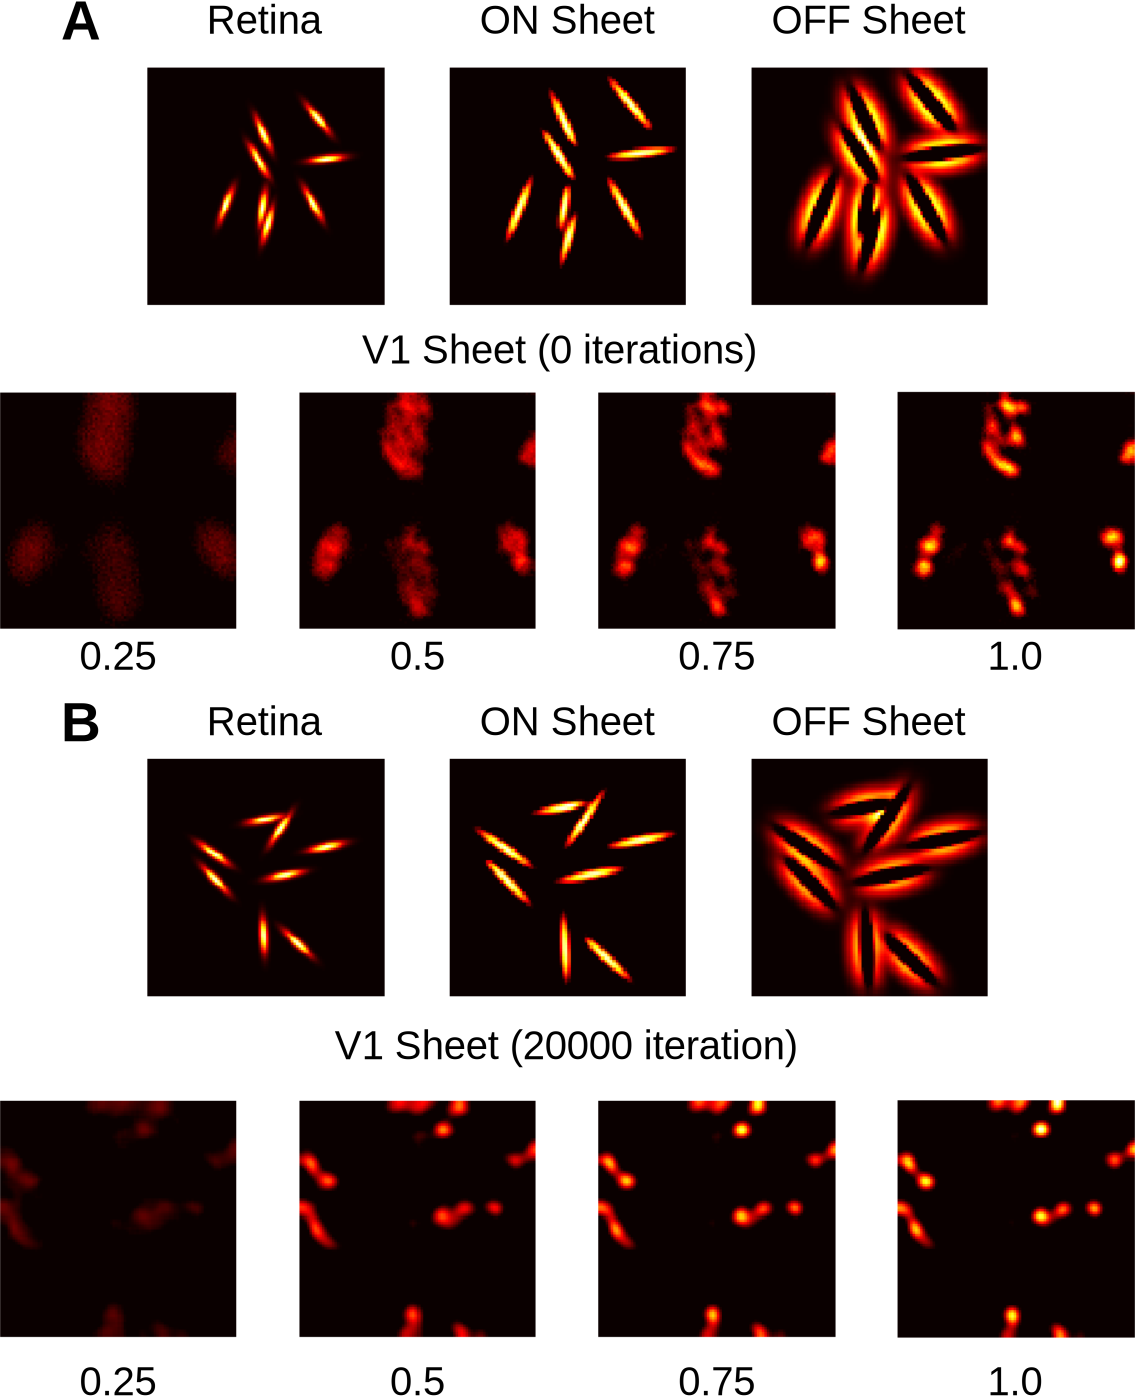
\includegraphics[width=0.8\textwidth]{./figures/GCAL_Activity_Bubbles.pdf}
\caption{{\bf Activity bubbles in response to training patterns in the
    GCAL model at the start and end of development (20000 iterations)}
  (A) Activity in the photoreceptor, ON, OFF, and cortical sheets in
  response to an example training pattern, at the start of development
  after the model is initialized. The process of settling is shown in
  the V1 sheet, eventually resulting in the formation of activity
  bubbles. Activities shown at $0.25$, $0.5$, $0.75$, and $1.0$ units of
  simulation time after the training pattern appeared on the
  photoreceptor sheet. Training patterns are updated every simulation
  time unit.  (B) Same plots for the photoreceptor, ON, OFF, and cortical
  sheets after $20000$ iterations of development. Bubble formation in
  the network is now much quicker and their positions are determined by
  the tuning properties of the units.}
  \label{fig:GCAL_Activity_Bubbles}
\end{figure}

Activity bubbles tend to center around the units with the strongest
afferent drive, as the long-range inhibition of the Mexican-hat profile
ensures competitive winner-takes-all interactions between bubbles. Each
bubble helps lead to smooth feature maps, in the same way that the
artificially imposed Gaussian activity in the Kohonen SOM helps maintain
the topological representation of the input. In general, smooth spatial
regions of postsynaptic activity make sure that units that are spatially
close in the cortical sheet will have similar feature preferences, due
to the action of Hebbian learning. Mathematically, this process can be
understood as a gradual rotation of the weight vectors (the unit weights
as a point in a high dimensional space) of the locally activated units
towards a particular direction in feature space driven by each training
stimulus.

The process of activity bubble formation varies over development as the
weights change. This can be seen by comparing Figures
\ref{fig:GCAL_Activity_Bubbles}A and B, showing the process before an
after development. Due to the random initial state, also seen at
iteration zero of figure \ref{fig:GCAL_Background_Development}B, bubble
are initially diffuse and take longer to form. Once tuning develops, a
selective V1 unit is able to quickly boost local activity via the
excitatory component of the Mexican-hat profile and suppress units that
are further away and competing with it. As a result, bubbles form
quickly and reliably in specific locations, as seen in
\ref{fig:GCAL_Activity_Bubbles}B. 

The effect of activity bubbles and the Mexican-hat profile can be seen
in Figure \ref{fig:GCAL_Background_Development} which shows development
of orientation maps and ON afferent weights in the GCAL model. The ON
weights show that the model has self-organized and that units are now
selective to oriented stimuli. Note that orientation maps appear early
on and are stable over time. This is quantified in the analysis
presented in Chapter \ref{chapter:GCAL}.

\begin{figure}
\center
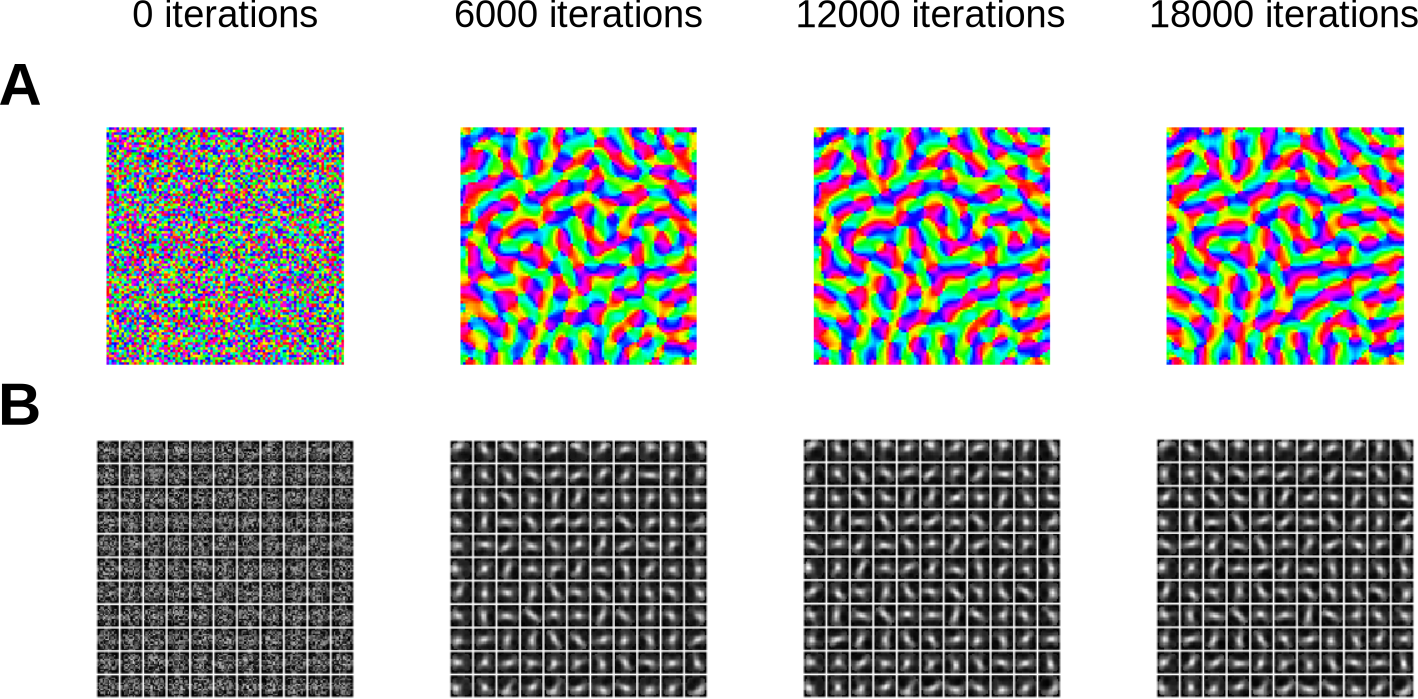
\includegraphics[width=0.8\textwidth]{./figures/GCAL_Background_Development.pdf}
\caption{{\bf Development of orientation maps and ON afferent weights
    from model initialization to $18000$ training iterations} (A)
  Orientation map measurements using the protocol from
  \citet{stevens_jn13} after $0$, $6000$, $12000$, and $18000$ training
  iterations. (B) Afferent weights from the ON sheet for $11\times11$
  regularly sampled units across the cortical sheet. Weights are
  initialized according to a uniform random distribution multiplied by
  the Gaussian envelope defined by Equation
  \ref{eq:GC_Gaussian_Weights}.  These weights then self-organize during
  the training process and the elongated shapes of these weight fields
  after development are indicators of the orientation preference and
  selectivity of the unit.}
  \label{fig:GCAL_Background_Development}
\end{figure}

\section{Conclusion}

%% jbednar: The background didn't actually discuss the diversity in the neural
%% population -- magno cells, parvo cells, other cell types, and their
%% properties (particularly temporal properties).  It would
%% have been good to do so, but probably no time now.
The visual system is composed of a large, diverse
population of cells with structure on both small and large spatial
scales. In addition, there are different types of dynamics on different
timescales such as the neural activity evoked by a particular visual
stimulus or the gradual developmental processes that shape the
functional organization of the cortex over time.

These different processes are recorded with different techniques such as
electrode recordings and voltage-sensitive--dye to record evoked
single-unit and population responses on short timescales and chronic
optical imaging of the intrinsic signal on long timescales. All of these
techniques capture different aspects of cortical function and ideally
all these techniques could be applied at once to record data over the
lifetime of a single animal.

It is possible to imagine a hypothetical experimental technique that can
chronically record the activity of millions of neurons with high spatial
and temporal resolution over the lifetime of a macaque animal
subject. Such a technique would be an extremely powerful tool for
understanding the dynamics of neural activity. In the absence of such a
technique, what is required is a theoretical framework that allows these
different sources of data to be integrated together, in order to
constrain a computational model of cortical operation.



\chapter{A reproducible workflow for exploratory research}
\label{chapter:reproducible_workflow}

Understanding visual processing in the primary visual cortex has been
the topic of intense research over the past fifty years, resulting in an
extensive literature spanning a wide array of different experimental and
computational techniques. Many different types of model have been used
to investigate the properties of visual processing, ranging from
theoretical models that tackle the propagation of visual information in
an abstract way, to mechanistic models that attempt to relate visual
processing to the neurons themselves.

As mechanistic models expand to account for more of the observed
properties of the visual system, they begin to pose some of the same
challenges to the computational modeler that the real biological system
poses to the experimenter. There is an overwhelming volume of raw
data that can be acquired from the subject of study, whether real or
simulated, and there is a myriad of ways in which this data can be
analyzed and visualized. As the number of model parameters and different
analyses grow, it becomes increasingly difficult to communicate results
clearly to the scientific community, threatening the integrity of the
scientific process.

All researchers need to be able to communicate their findings in order
to engage in the peer review process so that future researchers can
build on their work with confidence. It is crucial that researchers can
disseminate their findings to the rest of the scientific community in
way that is clear and understandable so that other researchers can
examine the core scientific claims. This is the basis of scientific
trust and as the number of steps involved in a research project
increase, the issue of scientific communication and reproducibility
becomes a primary concern.

Improving reproducibility in modern science is a problem that cuts
across disciplines. Many different areas of research now rely heavily on
computational resources for collecting, processing, and analyzing large
volumes of data. In other words, the challenge of achieving clear,
reproducible scientific communication is general and needs to be tackled
by the research community as a whole. One approach is to build
standardized tools to make the research process more efficient while
capturing the steps necessary to achieve reproducibility. The steps that
are captured then need to be communicated in a way that is clear and
meaningful.

The need for an efficient, exploratory, and reproducible workflow was
recognized early on in this project. Two concrete ways of improving
research efficiency and reproducibility were identified, resulting in
the creation of two new libraries for Python. Both the Lancet and
HoloViews projects are general purpose and freely available under an
open source license. This chapter describes how these two tools were
critical in ensuring that the simulations, calibration, and analysis
presented in this thesis were carried out in a maintainable,
communicable and reproducible way.

\section{Reproducibility of computational models}

Practical laboratory experiments are time-consuming and any procedure
involving animal subjects, especially primates, are extremely costly. It
is easy to understand why the process of reproducing a practical
experiment requires a significant investment of resources. Even when
replication studies are attempted, ambiguous results may persist due to
the effects of small sample sizes, uncontrolled idiosyncrasies between
experimental subjects, or miscommunication in the required steps.

The last point is particularly relevant to computational neuroscience
and is often the reason why modeling results are difficult to reproduce,
even though researchers working \emph{in silico} face fewer practical
issues. In theory, a computational model is specified precisely by code
that can execute reliably on any suitable processor.

Occasionally, there are practical concerns to consider. For instance,
there may be differences when performing numerical integration on 32 bit
or 64 bit hardware or there may be difficulties capturing the necessary
software state when trying to generate reproducible, high quality random
number streams. When these issues arise, they need to be carefully
addressed, but it is typically safe to assume that a working program is
an ideal, executable specification of some model.

If a program is an exact specification, why is there any issues of
reproducibility? The key problem is that an executable binary is a
specification aimed at the level of computational hardware, and that the
program source code only has to satisfy the constraints imposed by the
language compiler or interpreter. There are no guarantees that this
executable code can also be understood by a human, that the program
correctly implements the intended scientific specification, or that the
computation performed is scientifically meaningful.

This issue cuts to the heart of the distinction between reproducibility and
replicability, that is to say an external researcher's ability to
reproduce results exactly, as will be discussed shortly. A program
binary may be sufficient to achieve \emph{replicability}, but unless a
researcher can understand and manipulate this program at the scientific
level, this does not correspond to \emph{reproducibility}. It is when
considering the issue of reproducibility that proper scientific
communication is essential, as described in the next section.

\subsection{Reproducibility versus replicability}

So far the discussion has been framed using the word ``reproducibility''
but now that the concept known as ``replicability'' has been introduced,
it is necessary to define these two terms. In practice, these concepts
correspond to two different points along a continuous spectrum and both
properties are essential for the integrity of the scientific process.

Replicability is the notion that the results of an experiment should
remain exactly the same if repeated exactly. This means that the
hallmark of a replicable experiment is that other researchers are able
to repeat the claimed results by following the exact same set of
steps. In a computational context this might mean that a simulation can
be re-run given a particular binary file or given the appropriate source
code in an appropriately defined software environment. A simulation or
model may be considered replicable if sufficient information has been
made available to allow anyone to regenerate the relevant results.

Reproducibility is a broader concept with a greater overall value to the
scientific process. When a model is reproducible, the particular code
artifacts, software versions, random seeds, and other details of
implementation are not important. Instead, the goal is to establish
whether or not the scientific claims associated with the model follow
from the minimal definition. The aim is to explore the validity of the
scientific concepts underpinning the claims and to test the behavior
given different inputs in a way that is independent of implementation
details. As such, reproducibility is a better measure of scientific
correctness than replicability.

The merits of achieving replicability are currently under debate. Some
argue that replicability is an essential first step towards
reproducibility \cite{gent_corr13} and others argue that it is ``not
worth having'' due to lack of scientific value
\citep{drummond_icml09}. Still, if there were no cost associated with attaining
replicability or reproducibility, it is clear that scientific
research should ideally satisfy both properties.

In this thesis, replicability is viewed as an important initial step
towards the true goal, reproducibility. When one research group attempts
to build on work originally carried out elsewhere, achieving an
\emph{exact} match with the published values is crucial for establishing
confidence. Only by achieving an exact match with published results is
there any assurance that the code and software environment has been
configured correctly.

Having defined replicability and reproducibility, we can attempt to find
a workflow that makes it easier to achieve these two properties while
also improving research productivity. In particular, we will now
consider how the quality of a scientific output may be improved by
exploring how program correctness relates to the scientific tradition of
maintaining a research logbook.

\subsection{Logbooks and literate programming}

Before the advent of the computer, a scientist would often own a
handwritten logbook in order to track the steps taken over the course of
a research project. The importance of not leaving technical details to
memory has long been recognized; a concrete record is essential if many
highly technical steps is to be replicated at a later time.

Nowadays, not only is research recorded and disseminated electronically,
significant simulation and analysis code is a core component of many
research disciplines. Code itself is composed of a huge number of
discrete instructions specifying the computation of interest. Viewed in
this way, code is simply another set of research steps that need to be
recorded, making them a natural candidate for inclusion in a modern
electronic logbook format.

In many domains, code dominates the process of scientific analysis,
making it possible to invert this perspective and consider code as the
primary artifact. The question becomes one of correctness; does the code
satisfy the associated specification? A program that fails to perform
its desired function is incorrect as it fails to satisfy the
corresponding scientific intent.  In other words, the goal of
reproducibility is related to the goal of helping scientists write high
quality code to assist their research, as opposed to low quality,
incorrect code which if often detrimental. This is why making the code
needed to generate a publication freely available for review is
important for establishing confidence in the published results.

One approach known as ``literate programming'' introduced by
\citet{knuth_computerjournal84} aims to improve program correctness. The
idea is to interleave natural language text with the code so that a
programmer can explicitly state the thoughts behind the program, making
errors easier to identify. The text surrounding sections of code is
written in natural language to help the author clarify their thoughts
and to provide useful, high-level documentation to other people. With a
literate programming approach, it is often easier to maintain the
high-level specification in mind, making it easier to establish whether
or not any particular block of code fulfills its intended purpose. In
scientific research, this makes it easier to verify that the code is
correctly implementing its scientific intent.

This highlights the advantages of interleaving code with text, which may
include additional figures and mathematical equations, from two
different perspectives. From a code perspective, code is likely to be of
higher quality and more likely to fulfill its specification if it is
kept together with the corresponding high-level context. From the
perspective of reproducibility, such a document captures the code
necessary to execute the relevant research steps. We now examine the
strengths and weaknesses of a particular literate programming format,
namely the Jupyter Notebook.


\subsection{The Jupyter Notebook}

The ability to interleave code, text, and media content within a
notebook format has existed over a decade in the form of various
proprietary solutions, such as the Mathematica Notebook
\citep{wolfram_book03}. These attempts have suffered from restricted
interoperability and a lack of open standardization, limiting their
applicability and adoption. In more recent years, the Jupyter Notebook
(\textsf{jupyter.org}) has emerged as a popular, open source notebook
format that originated with the IPython project \citep{perez_cse07}. It
has since diversified in the set of languages it supports and the name
``Jupyter'' is designed to reflect the three core languages that can be
used in the notebook environment, namely, Julia, Python, and R.

The Jupyter Notebook interface is hosted in a web browser, which has
recently become feasible as a exploratory environment due to the
widespread adoption of the HTML5 
standard. The websockets protocol introduced in HTML5 has made it
possible to build rich, interactive browser documents that communicate
in a bi-directional manner with a local server. The notebook format
itself is based on the standard JSON format and can contain any of the
common media formats that can be displayed as part of a HTML web page.

Using well-established standards within a ubiquitous and
universal piece of software (the web browser) has been a major
factor in the success of the Jupyter notebook. Each notebook can contain
multiple sections of code interleaved with formatted text defined using
the Markdown markup language, fully rendered mathematical equations, and
raster and vector images, as well as client-side scripting using
JavaScript. This ability to interleave different standardized formats
within a single document is one of the biggest strengths of the notebook
format.

A live notebook session is simply a different way of working with an
interactive interpreter. The user is free to run any code, load data
from a file, and manipulate data structures in memory in an exploratory
way. By default, an ad hoc, interpreted session is not a replicable
artifact unless the history of commands is also recorded. Yet a
complete log of all commands ever executed is usually too verbose for
a human researcher to follow and understand.  The key difference
between a notebook and an automated command logging system is that users
can curate and refine the exact portions of code that need to be
recorded, while discarding everything else. The history stored in the
notebook can be made much clearer and much more meaningful than the full
history of every command that was executed.

Notebooks allow this type of free exploration but they also make it easy
to write and order blocks of code that can be interleaved with useful
explanatory material in order to build up an executable document.  The
idea is to build a notebook that, even after the state of the memory
is reset, is both readable and when executed from top to bottom,
regenerates all the desired visualizations, analysis, and data
structures. 

To achieve replicability, one can then use version control to track
the contents of the notebook and its dependencies. In order to achieve
reproducibility as well, the notebook also needs to express a clear
scientific intent and allow users to modify parameters and explore the
corresponding results.

Unlike the proprietary alternatives, the open
standards leveraged by Jupyter Notebooks helps ensure that this approach
is robust and does not rely on continued support of any particular
company. It is important that reproducible research is open, not only so
that anyone is free to test the core scientific claims but to allow
anyone to maintain the research artifacts over time without restriction.


\subsubsection*{Weaknesses in the ecosystem}

The Jupyter Notebook began as part of the IPython project and the Python
programming language remains core to the project, although other
languages can now be executed in the environment. Python has a strong
ecosystem for scientific computing that can be accessed from the
notebook, but the core, most widely used scientific Python libraries were
designed before notebooks became popular. This has left some particular
weaknesses in the value of Jupyter notebooks as reproducible, literate
documents.

One gap in the research process is in the ability to execute a large
numbers of independent processes. Such batch jobs are very common in
science; they may be used to split a large problem into many independent
pieces or to carry out parameter searches for optimization. Although the
IPython notebook does offer facilities for running shell commands,
process management in this way is difficult in the notebook environment.

As a result, it is common for researchers to switch to an entirely
different set of tools, such as shell scripts, when faced with the task
of launching and managing multiple program runs. Shell scripts are often
verbose and are rarely able to express the scientific intent of the
researcher in a clean, readable way. Exiting the notebook environment to
run batch jobs in this way leaves crucial research steps untracked,
reducing the replicability and reproducibility of the notebook document.

A second major weakness is in how data is presented and visualized
within the notebook environment. The matplotlib library
\citep{hunter_ieee07} is both mature and popular among Python users and
can be used inside notebooks. Unfortunately, this often leads to long
stretches of imperative plotting code which can quickly dominate the
notebook's content and becomes increasingly fragile as it expands. The
verbose and fragile nature of such code has a negative impact on
legibility, making it difficult to tell a clear scientific story.

Matplotlib was not designed with the possibilities of the notebook
environment in mind. The plotting API is not focused on generating
animated output, which was only made possible recently, and this library
is not capable of generating the sort of interactive web visualizations
that are possible using JavaScript. Without a visualization tool built
with the notebook environment in mind, notebooks are less readable and
less self-contained as long notebooks often break apart into small
pieces. This reduces efficiency, as well as scientific replicability and
reproducibility.

These problems are not inherent weaknesses in the notebook format, as these issues
can be addressed and improved upon by third party libraries. In
particular, the Lancet and HoloViews projects developed over the course
of this thesis have largely succeeded in solving these weaknesses.

\section{Lancet and HoloViews}

Both Lancet and HoloViews are designed to improve research productivity
and quality when working with Jupyter notebooks by minimizing the code
necessary to express a research task.  This makes it quicker for the
author to carry out their work while also making the notebook easier to
understand for the reader. By keeping the focus on the needs of the
researcher and away from the code itself, it possible to build notebooks
that are shorter, more legible, and more reproducible.

% Paragraph headings instead of enumeration?
Four general principles that have guided the design of both these
projects. These are: (1) to maximize research productivity by making
research tasks easy to specify, (2) to maximize the generality of each
project, making them as cross-domain as possible, and (3) to use
compositional primitives to maximize flexibility and expressiveness, and (4)
to use a succinct and declarative syntax, discouraging data mutation in
order to make reasoning about these data structures easier.

Maximizing research productivity is an essential goal for any tool
hoping to improve the reproducibility in a concrete way. Although the
majority of researchers do understand the importance of reproducibility,
their primary concern is to maximize their daily research
productivity. A tool that achieves perfect reproducibility but is
onerous to use or otherwise inefficient will not be chosen by
researchers and will be unable to improve scientific reproducibility in
practice.

Achieving generality is important for several reasons. Firstly, the
problems tackled by each library are not domain specific. Managing
batches of processes and visualizing data are common tasks faced by many
researchers across disciplines on a daily basis. Secondly, aiming at a
broad audience improves the chances that the library will be widely
adopted. With more users, there are more opportunities for constructive
feedback, more bug reports, and increased odds that additional developers
can be recruited to the project. Thirdly, aiming at a broad audience
ensures that the relevant terminology and documentation is kept simple,
understandable, and jargon free.

Keeping the project general also helps identify the points where
domain-specific flexibility is required, which helps maintain the focus
of the project on the general structure of the problem. The goal is to
always make it easy for users to easily adapt the code to their domain
specific needs. The last reason is that a general research tool can
serve the user better as there is often no telling which direction
research will go in. A general tool will remain relevant as the domain
specific research tools change over the course of a project.

Compositionality is the third core design choice. A well designed
compositional system can be flexible, expressive, and succinct, as long
as the semantics of the compositional operators are clear. Using a
compositional model, it is possible to achieve complex results using
simple, easily understood primitives. In addition, compositional
expressions can be constructed gradually, across multiple stages in a
notebook.

This offers more opportunities for interleaving explanatory material
between sections of code, further improving readability. Lastly, the
code defining the compositional primitives does not need to be modified
by the user and can simply be imported into the notebook
environment. This reduces the code required in the notebook itself,
keeping the bulk of the code separate, in a well-tested, third-party
library. Only the scientific \emph{intent} of the researcher should
remain in the notebook document, so that the final document only keeps
track of the steps specific to that particular research project.

Lastly, a declarative coding style in encouraged together with a
succinct syntax. In this context, this means that the internal state of
an object is specified when it is constructed and subsequent
modifications to this internal state are discouraged. This is closely
related to compositionality, as declarative atomic elements are easier
to compose together and reason about.  A declarative style makes it
possible to understand the state of an object when it is created,
without having to worry about code that might mutate this state later
on.


\subsection{Lancet: Managing sets of independent runs}

Lancet is a tool for specifying, launching, and managing large numbers
of independent process that is available publicly available
(\textsf{http://ioam.github.io/lancet}) under the BSD 3-clause
license. A paper describing Lancet was published in the Frontiers in
Neuroinformatics ``Python in Neuroscience II'' special issue
\citep{stevens_fninf13}. This paper has also been included in the
Appendix. Lancet was used to execute all the simulation batch jobs that
are analyzed in this thesis.

The main goal of Lancet is to allow batches of processes to be specified
and launched from Python in a succinct, declarative way. This makes it
possible to define a collection of simulations, launch them, and then
collect the results back into a Jupyter notebook, with the notebook
keeping track of all the steps involved. This avoids common, ad hoc
approaches that are not reproducible, such as the use of \texttt{bash} scripts to
execute jobs on a compute cluster.

The components of Lancet are designed to be as declarative as
possible. Each Lancet object is fully specified by the parameters of its
constructor and these parameters cannot be changed after the object has
been created. In addition, all objects have a complete, compact, and
readable textual representation. This representation is complete in the
sense that it is executable code that can be evaluated by Python in
order to recreate the same object in memory.

The core component types in Lancet are derived from three basic
classes: \tbf{Arguments}, \tbf{Commands}, and \tbf{Launchers}. Each
type nests into the next, with an argument object nesting into a command
which finally nests into a launcher. Arguments are used to specify
\emph{what} is to be run, such as a parameter space in a
\emph{tool-independent} and \emph{platform-independent} way. Once an
argument object is specified to define the batch arguments, it is passed
to a command object to specify \emph{how} these arguments are to be
executed in a \emph{platform-independent} but \emph{tool-dependent} way.

In practice, the definition of a command involves specifying which
software to be executed with the supplied arguments and how. This is
also the level where Lancet can be customized to support the execution
of new software tools. Lastly the launcher object is supplied with a
command containing the arguments in order to specify the computational
platform used for execution. A launcher is now a \emph{tool-dependent}
and \emph{platform-dependent} specification that can be called without
any arguments in order to launch a batch of processes.

The role of each of these component types will now be summarized with
reference to how they were used to run the simulations presented later
in this thesis. The analyses in Chapter \ref{chapter:GCAL} were based on
the simulations run for \citet{stevens_jn13}, which is an example of a
fully reproducible publication. These notebooks illustrate how Lancet is
used in practice, although the visualization and analysis portions of
these notebooks would have been better served by HoloViews, described in
the next section, had it been available at the time. The notebooks
necessary to reproduce the paper may be found at the following address: \newline
\textsf{https://github.com/ioam/topographica/tree/master/models/stevens.jn13}

\subsubsection*{\tbf{Arguments}}

The argument objects are the basic compositional components of
Lancet. They allow the compact, declarative definition of ordered
collections of arguments, where each individual argument set in the
collection will be passed to a single process. These objects compose
together using two operators: (1) the {\tt *} operator which defines the
Cartesian product between two argument sets, and (2) the {\tt +} operator
used for concatenation. Arguments offer a convenient way to specify
parameter spaces, and they were used to define the contrast robustness
analysis presented in Chapter \ref{chapter:GCAL}.

Two examples of Lancet argument objects and their composition are shown
in Figure \ref{fig:lancet_args}, extracted from the notebook used to
launch simulations analyzed in Figures
\ref{fig:L_model_metrics}--\ref{fig:GCAL_model_metrics}. Using the
\tbf{Args} class, it is easy to define a constant set of
arguments. Similarly, the \tbf{Range} class is suitable for defining a
range of regularly spaced argument values over a numeric interval. Here
it is used to define a range of $21$ different contrast values.

\begin{figure}
  \center
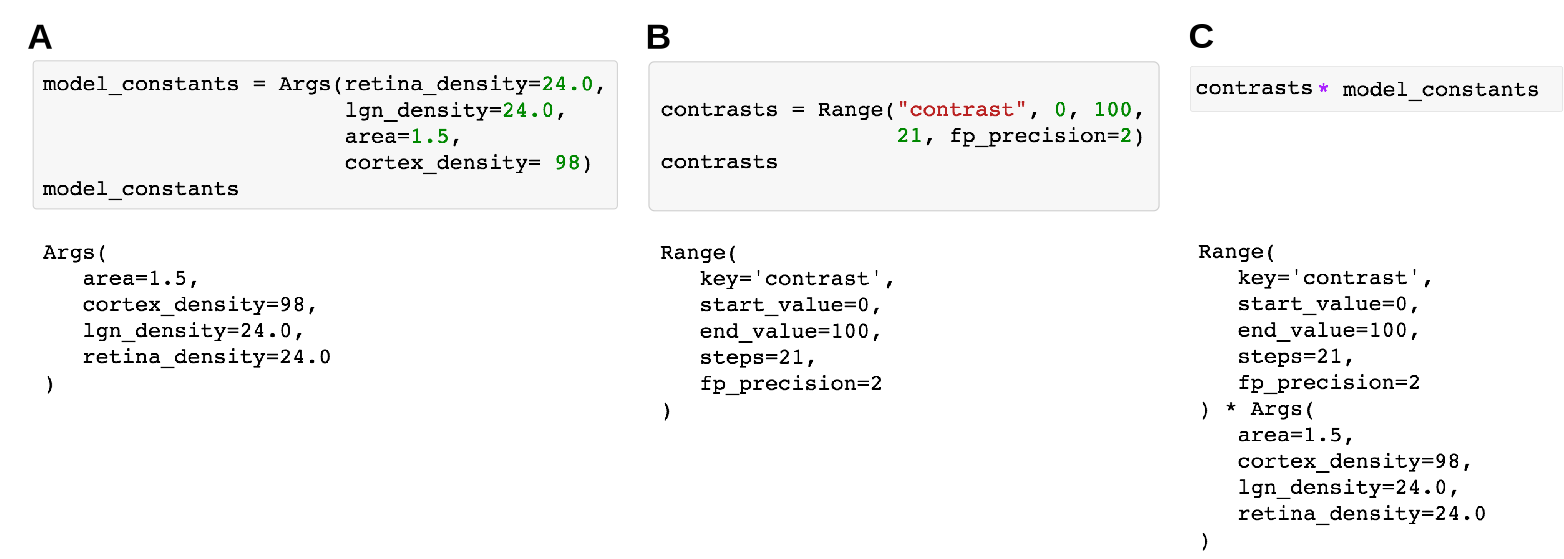
\includegraphics[width=1\textwidth]{./figures/Lancet_Args.pdf}
\caption{{\bf Examples of \tbf{Arguments} objects that were used to
    define the parameter space explored in Chapter \ref{chapter:GCAL}.}
  The Python code is shown on the top and the printed representation of
  the object is shown below. (A) This arguments object defines the
  simulation parameters that were kept constant by defining an
  \tbf{Args} object.  (B) A range of $21$ different contrast values
  spanning 0 to 100\%. (C) The Cartesian product of these two argument
  objects creates a new arguments object that specifies the $21$
  contrasts that are to be supplied to the command along with the fixed
  arguments.}
\label{fig:lancet_args}
\end{figure}


Applying the Cartesian product operator defines a new collection of $21$
arguments where each set contains one of the contrast values but also
includes the fixed constants declared in the {\tt Args}
object. Assigning handles to Lancet objects before composing them
together allows a declarative definition to be built incrementally over
the notebook, giving an opportunity to add text to describe each
individual component.

Note that all arguments values are always associated with a label. For
the constant {\tt Args}, these labels are specified via keyword
arguments whereas the single label ``contrast'' is used for the contrast
range. Taking the Cartesian product of these two arguments defines a new
object, which specifies the $21$ contrast values together with the
constant keywords. The textual representations of these object are clear
and readable, and once executed will recreate the object. This property
holds for all Lancet components and their compositions.


\subsubsection*{\tbf{Commands}}

Commands are objects that accept arguments, linking them to the
execution to a particular software tool. In other words, a command
defines how each set of named arguments will be used to invoke each
process in the batch. As it is impossible to explicitly support all
possible tools, Lancet makes it easy to define a new command class as
needed. This class only needs to return a list of string values to be
executed in the format accepted by the Python subprocess module.

By default, Lancet offers a generic and flexible command called the
\tbf{ShellCommand} that specifies how command-line programs are to be
executed. In many instances, using a \tbf{ShellCommand} is sufficient to
begin using Lancet. Nonetheless, it is recommended that a tool-specific
command class is used as (1) a specific command class can be
appropriately documented in a way that makes sense to the users of that
particular tool, (2) it encapsulates the invocation in a robust way
without relying on the specification of fragile string values, and (3) it
allows more sophisticated invocations of a tool, by generating input
files, for instance.

The Topographica neural simulator \citep{bednar_bmm08} used to execute
the simulations analyzed in Chapter \ref{chapter:GCAL} offers one such
example of a customized command class called \tbf{RunBatchCommand}. This
component makes it easy for Topographica users to run simulations using
Lancet by specifying a model definition file as well as a set of
specific analyses and measurements to be executed over the course of
each simulation run. All the measurements analyzed in Figures
\ref{fig:L_model_metrics}--\ref{fig:GCAL_model_metrics} were specified
in this way, including orientation preference and selectivity map
measurements, pinwheel analysis, and orientation tuning curve analysis.

\subsubsection*{\tbf{Launchers}}

The last type of component needed to run batch processes with Lancet is
the launcher object which encapsulates the computational platform used
to execute the command and associated arguments. By default, Lancet
offers two launcher classes, \tbf{Launcher} for running processes on a
local machine and \tbf{QLauncher} for running processes in parallel on a
Grid Engine compute cluster.

This separation between arguments, commands, and launchers makes it
easier to stay within the Jupyter notebook throughout an
investigation. At the start of a research project, it is typical to
start with some limited, local exploration that later expands to make
use of high performance computing infrastructure before
publication. Without Lancet, such a process would requires ad hoc
scripts or command-line invocations that change when working locally or
on a cluster. With Lancet, it is easy to define a \tbf{Launcher} and a
\tbf{QLauncher} together within one notebook, allowing the user to
quickly switch execution of the jobs from the local machine to Grid
Engine.

In simulations analyzed in Chapter \ref{chapter:GCAL} were all executed
using this approach. First a limited set of small simulations were run
locally and later many thousands of larger jobs were launched in
parallel on the Eddie cluster provided by the Edinburgh Compute and Data
Facility. These simulations generated hundreds of gigabytes of data on
disk that had the same organization on the cluster as it was locally.
This is the last key feature of Lancet that will now be discussed,
namely the way it helps you manage your files as part of a reproducible
workflow.


\subsubsection*{Tracking output files and reproducibility}

A common reason to running a batch of processes is in order to execute
side effects, with disk I/O being the most typical example. Manually
managing large collections of data files while tracking their provenance
is difficult and poses a barrier to reproducibility. Lancet helps users
keep track of any large data files that are generated outside the
Jupyter notebook by the launched processes. The details of how processes
were launched in the past are automatically recorded, and the way Lancet
executes commands consistently helps ensure a uniform organization for
all the output data wherever possible. For instance, the orientation map
analysis in Chapter \ref{chapter:GCAL} was derived from $842$
Topographica simulations which generated output data organized into
$842$ individual subdirectories.

One key concept is the notion of an ``output directory'', which holds a
collection of subdirectories containing the output of each run in the
batch. Given an output directory path, Lancet will ensure each process
is executed within a suitable named subdirectory and will also capture
all standard output to the \textsf{streams} directory. The naming scheme
applied to these directories may be customized, with the default scheme
combining a mandatory batch name with a unique per-job integer
identifier as well as the timestamp of when the jobs were launched. As a
single command object specifies how all the jobs of a batch are to be
invoked, each processes running in each subdirectory will have been
called in a consistent way. This in turn helps ensure that output data
within each subdirectory is generated consistently.

As Lancet manages the execution of all processes, starting from the
definition of the argument onwards, it can keep track of all the
arguments associated with each run and with the corresponding collection
of output files. A \textsf{.log} file is generated for each batch to
record the association from the unique per-job identifier appearing in
the subdirectory names to the explicit set of corresponding
arguments. This \textsf{.log} file holds information in a simple, human
readable format that can then be read back into the notebook using a
Lancet \tbf{Log} object in order to recreate the arguments used in the
original execution of that batch.

Next to the \textsf{.log} file in the output directory, Lancet stores an
\textsf{.info} file to store as much metadata as is available. Some of
this metadata may be specified by the user although Lancet also offers
helper utilities to make this process of generating metadata easy. For
instance, Lancet offers a \textbf{vcs\_metadata} utility that makes it
easy for a user to capture version control information in the
\textsf{.info} file. Other metadata is always stored automatically, such
as various timestamps and the textual representation of the launcher
object. As Lancet's objects are declarative, this representation is
executable and can be evaluated in Python to rebuild a launcher object
that is identical to one used to generate the original batch. This
launcher can then be called to execute the jobs once more, using the
same arguments, command, and launcher.

This concludes the description of Lancet and demonstrates how it helps
improve reproducibility by better capturing the researchers intent
without leaving Python. The key ways Lancet achieves this is by: (1)
improving the ease with which researchers can specify and launch batches
of jobs in Python, (2) recording the steps necessary to launch these
processes within the notebook environment, (3) encouraging a clear
organization of data files output by each process, and (4) automatically
storing metadata to trace the output of each process back to the
original arguments used to spawn it.

In order to be part of a fully reproducible workflow, Lancet must also
be used in conjunction with other essential research tools, and in
particular, version control. It is essential to use version control to
keep track of the notebooks themselves as they evolve, along with all the
associated support code and the versions of the tool that is being
launched. Large data files can be difficult to track properly but there
are dedicated version control solutions that are suitable for handling
large files, such as \textsf{git-annex}.

With Lancet, it is easy to build a productive and reproducible workflow
that lasts for the duration of a research project. It is designed to
work well from the Jupyter Notebook, encouraging a literate programming
style for reproducible research. Lancet makes it easier to launch and
manage jobs from Python, but if you also require greatly improved
visualization and analysis capabilities, you will want to use HoloViews,
described in the next section. In fact the \tbf{RunBatchCommand}
supplied by Topographica for use with Lancet outputs simulation data in
the form of HoloViews objects serialized to disk.


\subsection{HoloViews: Succinct visualization and analysis}

The success of a Jupyter notebook as a reproducible, literate document
is proportional to how much code can be \emph{eliminated} from the
notebook while keeping a complete record of the scientific intent and the decisions
relevant to the research task at hand. General-purpose code should be
moved out of notebooks whenever possible into properly tracked files or
into the broader Python ecosystem where it can be tested and
improved by large numbers of users.

In other words, the goal of a reproducible research notebook is to tell
a clear story that is focused on the task at hand, with as little
distracting code as necessary. Unnecessary code in the notebook not only
distracts the notebook author but it can derail later readers who wish
to understand the purpose of the document. Given that code in notebooks
tends to be less rigorously tested and more fragile, one way to improve
reproducibility is to eliminate all unnecessary code.

HoloViews is a new library ({\sf holoviews.org}) that I developed
together with Philipp Rudiger that greatly reduces
the custom visualization and analysis code required in a research
notebook. Like Lancet, HoloViews is compositional and designed to encourage a
declarative style, helping to compress large blocks of plotting code
into succinct expressions. It is also designed with the Jupyter notebook
in mind and aims to make interactive data exploration quick and
easy. The design of HoloViews is outlined in the \citet{stevens_scipy15}
paper, included in the Appendix.

When working with HoloViews, you do not need to write plotting code in
order to visualize and analyze your data. Instead, you declare data
structures that lightly bind your data together with the associated
metadata. These objects can very flexibly be nested and composed in different ways.
Then whenever the notebook environment requests the appropriate representation of
the data, a rich visualization is returned. In other words, HoloViews
helps establish a clear correspondence between how the way your data is
structured and how it is visualized.


\subsubsection*{HoloViews design principles}

HoloViews is not a plotting library, even though it does make building
complex, interactive visualizations easy. Instead, it is a library of
compositional data structures that lightly wrap the supplied data in
order to offer analysis methods as well as a rich visual
representation. Using the object representation as its visualization,
instead of relying on a separate plotting step, helps ensure immediate
visual feedback at all times.

This idea of immediately returning a human understandable representation
that represent an object in memory is not new. Interactive programming
sessions have existed for over half a century, although this type of
interaction has traditionally been purely text based. When working in an
interpreter, various data structures can be directly manipulated and the
changes can be immediately understood in terms of its textual
representation. For instance, the string representation of a float seen
by the user is not the same thing as the corresponding bytes in memory,
even though this distinction is not immediately obvious as the
translation is so transparent. HoloViews extends this idea of
transparent translation from data to representation to make data
visualization easy.

As Jupyter notebooks are hosted in the web browser, there are a host of
new formats that could be used to represent an object. HoloViews makes
use of the display hook system supplied by Jupyter Notebook to represent
objects in many different formats, including raster formats such as JPEG
and PNG, vector graphic formats (SVG), animated formats such as GIF and
MP4, and finally, interactive visualizations using JavaScript that are
only possible in the web browser.

As there are many semantic and esthetic choices that must be made in
order to generate a rich, high quality visualization, HoloViews makes it
easy to customize the properties of the visual representation associated
with each object. The way this is flexibility is achieved is to enforce
a separation between semantic information, the information \emph{about}
the data, and the plotting choices which is information about how the
data is to be rendered visually.


An example of how HoloViews is used in practice is shown in Figure
\ref{fig:HoloViews_GCAL_example}. In a single line of code, a richly
structured, composite HoloViews object is created that holds a complete
set of map measurements that were recorded over the course of a
simulation. This object appears in the notebook as an interactive
visualization: by moving the slider, the orientation selectivity and
preference measurement can be viewed at any simulation time for which
this measurement data is available. The line at the top of the cell {\tt
  \%\%opts Points (marker='s')} declares that this object is to be
visualized with pinwheel locations rendered with square
markers. Although this is a rich visualization, the object itself
\emph{is} the output data of the orientation preference, selectivity, and
pinwheel analysis. All data is available as full-precision binary arrays,
wrapped in a data structure with the textual representation shown in
Figure \ref{fig:HoloViews_GCAL_example}.

The line starting with {\tt \%\%opts} is not valid standard Python syntax but a
form of IPython-specific syntax called a ``magic''. These magics are
very convenient in the notebook environment, because they support additional
features such as tab-completion. Although HoloViews supplies these
magics, including tab-completion support, it is worth noting that
\emph{all} the features in HoloViews can be accessed in pure Python,
outside the notebook environment. This allows HoloViews to be run in
``headless'' mode to process data and generate visualizations without user
intervention which can be useful when running batch processes, e.g.\
when running Topographica simulations via Lancet.

\begin{figure}
  \center
  \includegraphics[width=0.9\textwidth]{./figures/HoloViews_GCAL_example.pdf}
  \caption{{\bf Example of how HoloViews can be used to explore a
      simulation of the model analyzed in Chapter \ref{chapter:GCAL}.}
    (A) Example of the simulation output at time $500$, run using the
    Topographica simulator. Both {\tt data.OrientationSelectivity.V1}
    and {\tt data.OrientationPreference.V1} are container objects that
    hold the output of orientation selectivity and preference
    measurements. {\tt PinwheelAnalysis} is an operation that can
    processes these types of container, annotating the orientation
    preferences with pinwheel locations using the method described in
    Chapter \ref{chapter:GCAL}. The top line {\tt \%\%opts Points
      (marker='s')} illustrates the HoloViews style system, in order to
    instruct the plotting code to render the pinwheels with square
    markers.  (B) The same notebook cell with the slider moved to
    display the results at a later simulation time (C) This shows the
    textual representation of the composite object that is displayed
    above, built up from the components described in this section. This
    object contains all the raw data output by the analysis and is
    composed of two {\tt HoloMap} objects, one of which is composed of
    {\tt Image} objects only, combined in a {\tt Layout} with another
    {\tt HoloMap} composed of {\tt Overlays} which in turn are composed
    of {\tt Image}, {\tt Contour}, and {\tt Points} objects}
\label{fig:HoloViews_GCAL_example}
\end{figure}


Figure \ref{fig:HoloViews_GCAL_example} serves to illustrate how the
various components of HoloViews interact in a real example that will be
dissected throughout the rest of this section. The way HoloViews can
build this type of complex visualization with minimal code will be
described in several stages, explaining how the visualization in Figure
\ref{fig:HoloViews_GCAL_example} is composed in several steps. First we
turn to how HoloViews defines semantic content.


\subsubsection*{Elements and Composition}

HoloViews is a library of atomic element classes that compose together
to form collections of elements called containers. Elements are named
according to particular visual representations, such as \tbf{Curve},
\tbf{Histogram}, and \tbf{Image}. These names serve to inform the
plotting system how data is to be rendered but also helps the user
construct a useful mental model regarding the dimensionality and
structure of the data. HoloViews makes it trivial to cast between
compatible elements types, keeping the binding between data and its
assigned element class as fluid as possible.

Elements accept raw data, accessible via the objects {\tt .data}
attribute but also encourage the user to associated meaningful metadata
with it. In particular, it is useful to supply semantic information
regarding with the dimensionality of the data, specifying a dimension
name and optionally units and allowable ranges. For instance, a
\tbf{Curve} may be supplied a list of tuple pairs and this data will be
visualization but it is useful to specify that the dependent dimension
is ``weight'' and the independent dimension is ``height'' in order to give
this data meaning. Once this \emph{semantic} information has been
supplied, the visual representation will be updated accordingly, for
instance, by labeling the x- and y-axes with ``weight'' and ``height''.

Given a number of distinct HoloViews objects, it is possible to compose
them together using the binary operators {\tt + } and {\tt *}. These
operators are used to organize data by building composite, indexable
objects. When considering the composition of elements, the crucial
distinction between {\tt +} and {\tt *} is that {\tt +} can always be
applied whereas {\tt *} demands the two components have matching
dimensionality. In the visual representation, the {\tt +} operator acts
to position two elements side-by-side whereas the {\tt *} operator acts
to overlays the first element with the second. When the {\tt +} operator
is used, the result is called an {\tt Layout} and when {\tt *} is used,
the result is called an {\tt Overlay}.

These features are illustrated in Figure
\ref{fig:HoloViews_GCAL_example}. First, the {\tt +} operator is used to
associate the orientation selectivity data with the orientation
preference data which is then shown side-by-side. The metadata
specifying the dimensionality of the data also appears in the
visualization. For instance, the orientation selectivity data is
labeled as {\tt Orientation Selectivity} which appear in the
corresponding title.

The leaf nodes of the data structure shown in Figure
\ref{fig:HoloViews_GCAL_example} C are the element objects, in this case
the set of elements types are {\tt Image}, {\tt Contours}, and {\tt
  Points}. These objects contain the raw analyzed data, so for instance,
the {\tt .data} attribute of the {\tt Points} object contains the exact
pinwheel locations as computed by the analysis. Alternatively, you could
compute the mean orientation selectivity without any loss of precision
given the corresponding {\tt Image} objects.

Now we have seen how compositional operators and the specification of
dimension metadata can be used to specify semantic content in a way that
is reflected in the corresponding visual representation. In the next
section, it will be shown how HoloViews also allows the customization of
all the visualization options that are purely esthetic and independently
of the semantic content.

\subsubsection*{Content and presentation}

HoloViews allows you to generate visualizations by constructing
semantically meaningful data structures around your data, avoiding the
need to write plotting code entirely. For this to work, HoloViews has a
style system that allows an object's visualization to be customized
without having to store this style information on the object itself.

This design is similar to the recommended separation between content and
presentation in HTML and CSS, allowing visualization options to be
easily changed without affecting the content. This approach makes it
easy to immediately visualize data using the default visualization
settings and then customized its appearance as a separate step later on
in the notebook.

When the notebook environment requests the appropriate representation of
an object, the HoloViews object is automatically passed to the
appropriate plotting classes in the background. There, the style system
makes use of a unique integer ID on the object to determine the
appropriate style options. These styles are supplied by the user as
keyword arguments to be passed directly to the appropriate plotting
call.

To illustrate, when using the matplotlib plotting library
\citep{hunter_ieee07} as a plotting backend, a particular {\tt Points}
object may have a style associated with it, specifying the marker with
the keyword pair {\tt marker='s'} as shown in Figure
\ref{fig:HoloViews_GCAL_example}. The integer id on the object is the
only link necessary between the semantic content of the object and the
style system and both the key ({\tt marker}), and the value ({\tt 's'}),
are defined by the matplotlib plotting API, and not by HoloViews.

The way HoloViews passes style information to the plotting classes is
entirely general and entirely independent of any particular plotting
library. For this reason, HoloViews is able to support multiple plotting
backends, where matplotlib is only the default option. The Bokeh library
\citep{bokeh_manual} is also supported by HoloViews as a separate
backend, allowing for even more interactive visualizations in the
browser.

The separation between presentation and content and the separation
between HoloViews and the various backends further illustrates why it is
incorrect to think of HoloViews as a plotting library. In terms of
visualization, it acts more like a common interface for rapidly viewing
data in notebooks that makes it easy switching between different
underlying plotting libraries.


\subsubsection*{Immediate, interactive, and exploratory visualizations}

Using the style system together with elements, layouts, and overlays
allows HoloViews to quickly generate static plots that could also be
defined with blocks of imperative code using a plotting library. Perhaps
the most compelling reason to use HoloViews in the Jupyter notebook is
for its flexible and general system for interactive data exploration.

In addition to the composition operators introduced in the previous
section, elements can be grouped into high dimensional containers for
instant interactivity. The core container type, called the {\tt HoloMap}
may be thought of as high dimensional dictionary that allows the user to
scrub through the set of keys with a JavaScript slider in order to
browse the elements it contains.

As with all HoloViews data structures, {\tt HoloMaps} can be composed
using the {\tt +} and {\tt *} operators and accept additional metadata
to specify the dimensionality of the space in which the elements
reside. Keys are specified as n-tuples, where each position in the tuple
corresponds to the value of a particular dimension of the container
associated with the value. {\tt HoloMaps} can be visualized as animated
GIFs, as video using MP4 but most commonly, they are rendered as
interactive visualizations where they key dimensions define
corresponding JavaScript sliders as seen in Figure
\ref{fig:HoloViews_GCAL_example}A and B.

{\tt HoloMaps} offer an extremely convenient and flexible way to explore
data. Any software can integrate with HoloViews by returning {\tt
  HoloMap} objects making it easy to explore results in the notebook. As
all HoloViews objects are thin wrappers around the data, this is a
powerful way of simultaneously processing data and generating the
corresponding visualization at the same time. In addition, it is easy to
build operations that accept {\tt HoloMap} objects as input in order to
generate a new, derived {\tt HoloMap}. This makes it possible to build
data processing pipelines using HoloViews operations and this is the
approach used by the Topographica neural simulator
\citep{bednar_bmm08} for the visualization and analysis code.

Figure \ref{fig:HoloViews_GCAL_example} shows an example of this
approach. The {\tt data} variable is output by the measurement code in
Topographica that integrates with HoloViews and {\tt PinwheelAnalysis}
is an operation that locates the pinwheel singularities
from orientation preference maps, generating a new {\tt HoloMap} of the
analyzed data. This {\tt HoloMap} is composed of {\tt Overlays} objects
which are same type of object as created by the {\tt *} operator. These
overlays have the original orientation map image on the bottom layer,
overlaid with the real and imaginary contours of the polar
representation (shown in white and black respectively) and then finally,
the points marking the identified pinwheel locations. The exact analysis
data is held by these objects, computed using the methods of
\citet{lowel_ejn98} and described in more detail in Section
\ref{section:map_metric_in_simulations}.


The overall data structure shown in Figure
\ref{fig:HoloViews_GCAL_example}A is an example of a {\tt Layout} of
{\tt HoloMaps}, which allows data to be interactively explored with
widgets across multiple {\tt HoloMaps} in the same way as they can be
explored individually. In this figure, the widget traverses the dimension
associated with the {\tt HoloMaps} keys, namely simulation time. Both
subfigure A and B display the same notebook cell but with the slider
moved from a simulation time of $500$ to a simulation time of
$2500$. Using {\tt HoloMaps} make it easy to interactively explore
entire data sets in this way.

The style system directly applies to elements within HoloMaps, also
illustrated in this figure. The default marker style for pinwheels is
circles, as seen later on in Figures
\ref{fig:L_model_metrics}-\ref{fig:GCAL_model_metrics}. In this example,
the keyword {\tt marker='s'} has been passed to the matplotlib backend
for rendering the {\tt Points} objects in the {\tt HoloMap}, switching
the points to use square markers across the {\tt HoloMap}. Note that the
style information regarding this choice of marker is stored separately
from the object itself, which is why this information will not appear in
the textual representation of the object of the sort shown in
\ref{fig:HoloViews_GCAL_example}C.

\section{Discussion}

In this chapter, two new libraries have been introduced that have
greatly improved research efficiency and productivity in the Jupyter
notebook. Framed this way, these projects are not primarily about
achieving scientific reproducibility. Paradoxically, not focusing on
reproducibility is a crucial
feature for any reproducible approach to gain traction, as without a
clear, pragmatic incentive, users have no reason to switch to a more
reproducible workflow. There need to be clear productivity advantages
before researchers engaged in less reproducible practices will be
willing to switch to better work patterns.

One of the issues with reproducibility is that it is often perceived to
be in opposition to research efficiency. For instance, researchers are
known to invest time and effort in order to make their work available
and reproducible after publication. Reproducibility is generally
understood to be important but it is also seen as an additional burden
to an already challenging research process.

The core philosophy underpinning the projects presented in this chapter
is that, in the right context, research efficiency can serve to
\emph{improve} reproducibility. A lot of the difficulties regarding
reproducibility in computational neuroscience stem from workflows that
are ad hoc, unmaintainable, and inefficient. A solid workflow is one that
with practical benefits by making the research process quicker, easier
and more maintainable. Approaches that aim to improve reproducibility but
that prove inefficient or onerous to use will fail to gain traction.

Reproducibility is recognized as important across the research community,
but many do not see the practical benefits of reproducibility as part of
the daily research process. An experienced programmer will comment code,
not just to assist other people but to aid their own understanding at a
later date. Similarly, a researcher who uses version control to track
concise, well-structured notebooks will find that, not only is their
research easier to communicate with others but that their regular
workflow has also become easier to manage.

Both Lancet and HoloViews are designed to allow a researcher to express
their intent as succinctly and efficiently as possible. As a result, not
only can you do more with less code, you more functionality can be
included in a single, self-contained notebook while presenting a clear
scientific story. Together with version control, the adoption of clear,
well-written notebooks as readable, literate documents will go a long
way towards improving scientific reproducibility.

To date, HoloViews has been a very successful open source project with a
more general scope than Lancet and a correspondingly greater
adoption. It won in its category in the UK Open Source Awards 2015 and
is now in use by researchers worldwide, both in computational
neuroscience and in other fields. For instance, it has been used as
part of an EdX online course in 
condensed matter physics (\emph{Topology in Condensed Matter: Tying Quantum
Knots}). This made use of an extension to HoloViews to support plots
generated by \texttt{qutip}, the ``Quantum Toolbox in Python''.
It has also generated plots used in several physics publications
\citep{nijholt_arxiv15,tenner_apchd16}. 
In addition, HoloViews has been extended to create a new project called
GeoViews with support from the U.K. Meteorological Office (Met
Office).  GeoViews adds support cartographic projections for exploring
geographical and meteorological datasets.

These examples serve to show
that HoloViews is an entirely general tool, growing in popularity, which
can support researchers from the initial exploratory research stage to
final publication. The adoption of Lancet has been more limited, but it
has been used by other researchers to launch microprocessor simulations,
again helping to demonstrate the generality of the approach
\citep{elver_hpca14}.

All the code used in this thesis is publicly available and under an open
source license (BSD 3-clause), including the Topographica simulator and
all dependencies. The work presented in Chapter \ref{chapter:GCAL} is
based on a fully reproducible publication using Jupyter Notebooks
\citep{stevens_jn13}. These notebooks demonstrate the use of Lancet to
manage and execute simulations from Python, but predated HoloViews. Had
HoloViews been available at the time, the work necessary to generate
reproducible figures would have been dramatically reduced. The notebooks
associated with this paper are available from \newline {\sf
  https://github.com/ioam/topographica/tree/master/models/stevens.jn13}.


\section{Conclusion}

Lancet and HoloViews are general, open source research tools that
enhance both scientific productivity and reproducibility. By allowing
researchers to declare their intent with less code within a literate
programming environment, specifically the Jupyter Notebook, data can be
rapidly generated, visualized, and explored in a more reproducible
way. This results in a more powerful, more efficient, and more enjoyable
scientific workflow.

The general design of these tools has led to them being adopted by
scientific researchers across the world and across disciplines. Although
HoloViews was essential for enabling the work presented in this thesis,
the generality and flexibility of the design means that the same tool
that enables rapid, interactive data exploration has also been used to
generate published visualization in an entirely different field, namely
quantum physics.

\chapter{Dynamics of the evoked response across spatial scales}
\label{chapter:SIRD}

Understanding how neurons respond to a sequence of visual images is
crucial for establishing the function of the primary visual cortex
(V1). In this thesis, the aim is to build a mechanistic model that can
account for the spatiotemporal responses of neurons in macaque monkey
V1 across a wide range of both spatial and temporal scales. To make
initial progress towards this goal, in this chapter we will focus on
understanding the time course of neural activity in response to a
brief stimulus (a peri-stimulus time histogram, or PSTH).  Later
chapters will then consider how these responses vary in the long term,
over the course of development.  Thus for the purposes of this
chapter, we will consider response properties to be a fixed function
of a neuron's inputs, not simulating any plasticity or development.

Despite the many years of study of V1 using different experimental
techniques, characterizing how a population of neurons responds even
to a simple visual stimulus turns out to be surprisingly difficult.
The main reason is that there is no single technique that can
accurately measure the firing rates of the many individual cells that
make up a large population.  Single-unit electrophysiology can very
accurately record the spiking activity of individual neurons
responding to a stimulus, but even large electrode arrays can only
return information from a very sparse sampling of the cells present.
Voltage-sensitive-dye optical imaging (VSDI) provides complementary
data, reporting temporally precise information about membrane voltage
from very large numbers of cells, but lacks the spatial accuracy to
resolve individual neurons, instead integrating indiscriminately
across neural tissue that includes many different cell types, \emph{en
passage} fibers, etc.

Because these two techniques are measuring quite different quantities,
it is not surprising that the results from such studies differ
dramatically. As shown below, single-unit studies indicate that
individual neurons have sharp, transient responses, yet population
measurements indicate slow, gradual, sustained responses for the
population as a whole.  Resolving this discrepancy is the focus of this
chapter, because it will allow us to relate single-unit and population
data to characterize how a densely connected network of neurons responds
to a stimulus over time.  In a series of steps, I will show how to extend the
well-validated IRD model \citep{albrecht_jneurophys02} of single-unit
responses into a model for the population as a whole that is compatible
with both the single-unit and VSDI data.

Specifically, three new mechanisms needed to be added to the
single-unit model, each accounting for a particular feature of the
VSDI signal. Each mechanism is introduced only when necessary, using
the simplest mathematical formulation consistent with the experimental
data. The result is the first spatially extended, mechanistic account
of the voltage-sensitive--dye signal.

This model is distinct from previous work on the VSD signal that has
focused either on modeling the detailed spiking biophysics within the
extent of a single VSDI pixel \citep{chemla_neuroimage10}, or on
modeling the spatiotemporal dynamics in terms of the bulk electrical
properties of the tissue, without reference to single-unit responses
\citep{sit_neuron09}. In contrast, the model presented in this chapter
has a simple mathematical formulation that shows how the firing rates
of individual neurons are transformed by the structure of the network
in a mechanistic way. This implementation will serve as a
reference for the spatiotemporal developmental model to be presented
in Chapter \ref{chapter:TCAL}.

The sections below analyze the differences between single-unit
responses characterized by the IRD model, population responses from a
diverse collection of neurons each characterized by the IRD model, and
a spatially organized population with spatially dependent responses.
Each section builds incrementally on the IRD model, introducing one
new mechanism in turn, along with the experimental data that motivates it: (1) latency
scatter, which effectively stretches out the time constant of the VSDI
signal compared to individual units, (2) spatial variation in latency
with respect to the stimulus center, and (3) diversity of
tuning dependent latency across units.
Together these mechanisms characterize
important types of diversity of the units in the real neural population,
and the resulting model is able to predict accurate VSDI responses
from the single-unit activities, allowing us for the first time to
illustrate how each of the experimental techniques relates to the underlying
neural activities.

\section{Dynamics of electrical and optical responses}

Single-unit electrophysiology allows precise measurement of the
activity in a small neural population with a high temporal resolution,
whereas optical imaging measures the overall activity across an extended volume
of neural tissue (see section \ref{section:evoked_background} for
detailed background). Data obtained using electrophysiology is often easier
to interpret, since it is a direct measurement of the cell's
electrical activity, whereas voltage-sensitive imaging more indirectly
conveys the bulk response of the tissue.  However, it is very
difficult to infer properties of the whole population from the sparse
and biased sample of single-unit data available, and so both types of
evidence are invaluable.

Figure \ref{fig:SIRD_comparison} shows results from both methods,
including PSTH profiles fit to single units by the IRD model, and VSD
responses for similar stimuli.
%%
\begin{figure}
\center
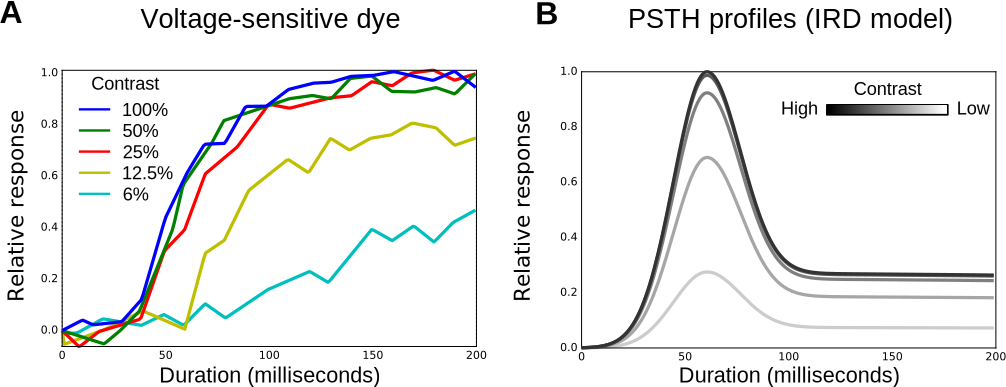
\includegraphics[width=1\textwidth]{./figures/SIRD_comparison.pdf}
 \caption{{\bf Temporal onset profiles recorded using voltage-sensitive
     imaging are qualitatively different from temporal profiles of
     single-unit spiking data in macaque V1.} (A) Normalized
   voltage-sensitive--dye response for the five contrasts indicated by
   the color key for the central region of interest in
   \citet{sit_neuron09} that was marked in Figure
   \ref{fig:sit_data}C. (B) Normalized PSTH profiles generated by the
   IRD model of \citet{albrecht_jneurophys02} for five contrast values
   chosen to match the corresponding voltage-sensitive--dye amplitudes
   for easier comparison. The resulting onset times for both types of
   data are similar, but the PSTHs quickly reach a peak and then decay,
   while for this constant stimulus the VSDI signal slowly reaches a
   plateau.
}
\label{fig:SIRD_comparison}
\end{figure}
%%
Both plots show neural responses evoked by similar stimuli of various
contrasts presented for $200$ milliseconds, one measured
electrophysiologically, and the other with VSDI.  The VSDI results are
measured from the retinotopic location corresponding to the stimulus,
so that they will be comparable to the single-unit PSTH data.

There are some very broad similarities between the two experimental
data sources shown in Figure \ref{fig:SIRD_comparison}. Both
signals first rise at a roughly similar time (though slightly later
for the VSDI response). In both, low-contrast stimuli
lead to slower responses and a lower overall response amplitude.
Responses for both types of signal saturate with contrast, as
neurons approach their maximal response rate for higher contrast
levels. This response saturation is well approximated by the
Naka-Rushton equation given in Equation \ref{eq:IRD_amplitude}
as the contrasts used in B only differ from the corresponding contrasts in
A by a constant multiplicative factor.

However, in nearly every other respect, the two types of profile have
very distinct temporal properties.  The most obvious discrepancy is that
the VSD response gradually approaches a plateau reached only by $150$ or
$200$ milliseconds, while the PSTH profiles each peak within the
first $75$ milliseconds. I.e., the optical signal monotonically rises
throughout the response, while the firing rate rises and then falls
dramatically. There is also a small mismatch in the onset time, with
these PSTH profiles rising slightly earlier than the
voltage-sensitive--dye responses.

One way to express the difference between results from each method is
in terms of varying time constants, by analogy to various
physical systems exhibiting hysteresis or damping. The single-unit PSTH
profiles rise and fall rapidly around the peak, indicating that the
firing-rate response has a low time constant. Conversely, the changes
in the voltage-sensitive--dye response occur more gradually, suggesting
that a large time constant is associated with the population-level
interactions reflected in the VSDI signal.

This larger time constant is not a property of the voltage-sensitive--dye
itself, which is able to transduce fluctuations in electrical potential
within a few milliseconds \citep{chemla_jphys10}. The non-linear
relationship between membrane potential and spiking activity also cannot
account for this discrepancy, as the incoming afferent activity from the
LGN already has a strongly peaked PSTH profile. Because changes in the membrane
voltage are driven by spiking input received synaptically, the fact
that the afferent input from the LGN cells also has a clearly peaked PSTH
profile suggests that the membrane potential for individual cells will
also have a similarly peaked shape. Figure \ref{fig:LGN_PSTH_maunsell} showed the firing-rate
responses for magnocellular and parvocellular LGN neurons recorded from
macaque \citep{maunsell_visneuro99}, indicating that a peaked response
applies to both the spiking input and spiking output of cortical neurons.
%jbednar: It would be stronger to show a peaky plot of membrane potential
% for V1 neurons in response to a step stimulus, though!
% E.g. intracortical synaptic input could conceivably change the
% shape too, since it is delayed in time, which would change the
% membrane potential directly, even without averaging over bulk
% tissue as in VSDI.  And the inputs, if coming from a variety of
% lags, could easily be smeared in time.

In addition to the differences in the temporal profiles for neurons at the center
of the response, there are spatially dependent effects at the population
level that also require explanation. Figure \ref{fig:ST_gradient}B shows
the spatiotemporal analysis of the VSD response for two different
contrast conditions, reproduced from \citet{sit_neuron09}. There is a
variation in latency across space that is time dependent, with a nearly
simultaneous onset across cortical space but a diverging latency to
the peak response. In Figure \ref{fig:ST_gradient} this phenomenon is
indicated by the increasing spatiotemporal gradient, marked by the
dotted black lines at different points in the response.  These effects
also vary as contrast is reduced, which will be discussed near the end of
this chapter.
%
% Also, always remember the 4 S's. Every figure with experimental data
% *ever* *always* needs to say the Scale, Species, Source (citation),
% and Spot (brain region). The last one's a bit of a stretch, but
% maybe that will help you remember it.
\begin{figure}
\center
\includegraphics[width=0.9\textwidth]{./figures/ST_gradient.pdf}
\caption{{\bf Increasing spatiotemporal gradient over the course of the
    VSDI response in macaque V1.} (A) Analysis region boundaries overlaid on top of the peak
  response to the stimulus at 100\% contrast. The optical response is
  averaged for each pair of successive annuli at each distance from the
  center. Each of these mean responses over time gives the data for one row of the
  spatiotemporal plots on the right. (B) Spatiotemporal plots for the
  100\% and 25\% contrast conditions. At the point where evoked activity
  is first detected (a), the response appears almost simultaneously
  across cortical space. Part way through the response (b), a
  spatiotemporal gradient emerges. Lastly as the response starts to
  plateau (c), there is an increased spatiotemporal gradient. In
  other words, the response in the more distal regions takes longer to
  plateau than the response in regions near the center.
  The three dashed lines are shown at the same
  position in the two plots, making it clear that the overall response
  is also delayed in the lower contrast condition. Adapted from
  \citet{sit_neuron09}.}
\label{fig:ST_gradient}
\end{figure}

So far we have been focusing on the stimulus onset, even though the offset response
data is also available in \citet{sit_neuron09}. For two main reasons,
only the duration of fixation after the stimulus onset will be
considered in this chapter. First,
the IRD model is only defined for stimulus onsets. Second, there is
much more experimental data regarding onsets than offsets, and in
particular all the data presented in this chapter were recorded with
respect to stimulus onset. In any case, there are clearly dramatic
differences in the onset responses between the two experimental
techniques that require explanation.

\subsection{Relating the response signal across scales}
\label{section:response_across_scales}
% jbednar: can probably shorten this section; it's a bit repetitive
% with the intro.
The VSDI response and the firing response profiles described by the IRD
model are a reflection of neural response at two very different
scales. The optical response reflects the activity of a large, diverse
neural population whereas the IRD model captures the typical firing rate
responses of individual cells. The differences in the two response types
shown in Figure \ref{fig:SIRD_comparison} are therefore related to
understanding the properties of the response for different neural
population sizes and across different spatial scales.

The challenge of bridging across these different scales can be tackled
either by a top-down experimental approach or a bottom-up modeling
approach. The experimental approach would be to observe the activity at
the population level and use a combination of experimental techniques to
identify and quantify the different contributions from the elements of
the population, such as different cell types, synaptic inputs,
connectivity profiles, etc.  Such an approach is becoming more
feasible due to new genetic and imaging techniques, but is still a
long way from being truly practical, particularly in macaque.

The bottom-up modeling approach is to start with a description of the
single-unit responses and to consider a large population of such
neurons, incrementally adding diversity or new mechanisms to this
population to account for additional types of cells or interactions,
until the resulting model approximates the VSD signal.  This chapter
takes the latter approach, starting with a population of IRD model
units to capture the observed responses of single neurons.  At first
this population will be entirely homogeneous, with every unit
responding in exactly the same way. This will result in an aggregate,
population response with exactly the same temporal response properties
as individual neurons, which is clearly not the case in animals.

Of course, real neurons in a population are not homogeneous in their responses, due
to differences in their intrinsic properties, structural variations in
their connectivity, and their different tuning properties. It is
also important to recognize that the IRD model captures the single-unit
responses of a subpopulation of neurons that respond to a specific
stimulus protocol. No experimental procedure can capture the full
diversity of all possible responses across a neural population, and it is
necessary to study the methods used to understand the explicit and
implicit biases that result. In other words,
the particular details of the stimulus protocol used to calibrate the
IRD model have crucial implications regarding the types of responses that
are adequately captured by this model.

Note that the IRD model is a high-level, descriptive model that maps from an input
of a specified contrast to a cortical firing-rate response profile
comparable to experimentally measured PSTH curves. It does not model
specific input patterns or processing of those patterns by circuitry in
the eye and LGN, and so it cannot directly relate the activity across
cortical space in terms of the retinal image.  Instead, it is designed
to fit only the response for a stimulus well matched to this
particular neuron's preferred retinotopic location and pattern shape,
including orientation preference.

The task of this chapter is to consider the IRD model as a summary of
single-unit responses and to ask how these responses may diverge across
a population. By considering different types of such diversity, it will be
shown how to generate a population of neurons whose temporal responses
are governed by the IRD model but which together can account for and
predict the observed VSDI signal when the activities are pooled
together.  Each new addition to this population yields a qualitative
change in the simulated spatiotemporal response, eventually bringing it
in line with the observed VSD dynamics.

The following mechanisms will be considered in turn: (1) latency scatter
to explain the increased time constant of the VSDI signal relative to
the single-unit PSTHs, (2) spatial variation in latency with respect to
the stimulus center, which is then combined with (3), diversity in
latency due to the variable tuning properties of the different cells in
the population.  The resulting model then explains both the
spatiotemporal gradient shift as well as the extended plateau in the VSD
signal response, showing how individual cells can have responses
well-characterized by the IRD model yet the overall population responds
as in the VSD imaging.


\section{The time constant of the population response}

In order to understand the time constant of the voltage-sensitive--dye
imaging signal, it is worth considering the simplest form of temporal
diversity missing from the IRD model. Given a particular contrast and
set of model parameters, the IRD model always outputs a fixed
description of the corresponding firing response profile.

A collection of PSTH recordings from multiple cells are not all the same
as the profile used to summarize them, varying in response amplitude,
shape, and latency. In order to explain the temporal properties of the
population response, it makes sense to consider the response latency
spread across the different neurons. As a basic intuition, it would make
sense for the population response after averaging across a temporal
spread to act with an increased time constant. This hypothesis is
examined next.


\subsection{Latency scatter across the cortical population}
\label{section:latency_scatter}

In order to decide on an appropriate distribution of latency scatter
across a population of IRD units, the first step is to considering
whether a diversity of responses could be generated by the IRD model
itself. The curves shown in Figure \ref{fig:SIRD_comparison}B used the
mean parameter values of the IRD model defined in section
\ref{section:IRD_background}, but the standard deviations of these
values were also published. This suggests a way to generate a diversity
of curves using the IRD model itself.

I.e., you can model model the variation of a parameter given its mean and
standard deviation by simply using a Gaussian distribution. By sampling for
each parameter of the IRD model from a Gaussian probability distribution
with the appropriate mean and standard deviation, it is possible to
obtain a diverse population of IRD PSTH curves from which a latency
scatter histogram can be derived.

Figure \ref{fig:sird_calibration_latency_scatter}A shows the relative
onset distribution of the IRD model as inferred from $1000$ profile
samples assuming normally distributed parameters. The means and standard
deviations used are as stated in \citet{albrecht_jneurophys02} and are
available in section \ref{section:IRD_background}. For the purposes of
validation, this distribution is shown next to an experimental onset
distribution recorded directly from macaque V1 in Figure
\ref{fig:sird_calibration_latency_scatter}B \citep{nowak_visneuro95}.

% jbednar: Plot C should be explained clearly; I though it was for the
% scatter in A, but it's for the red scatter in B, right?  A bit confusing.
\begin{figure}
\center
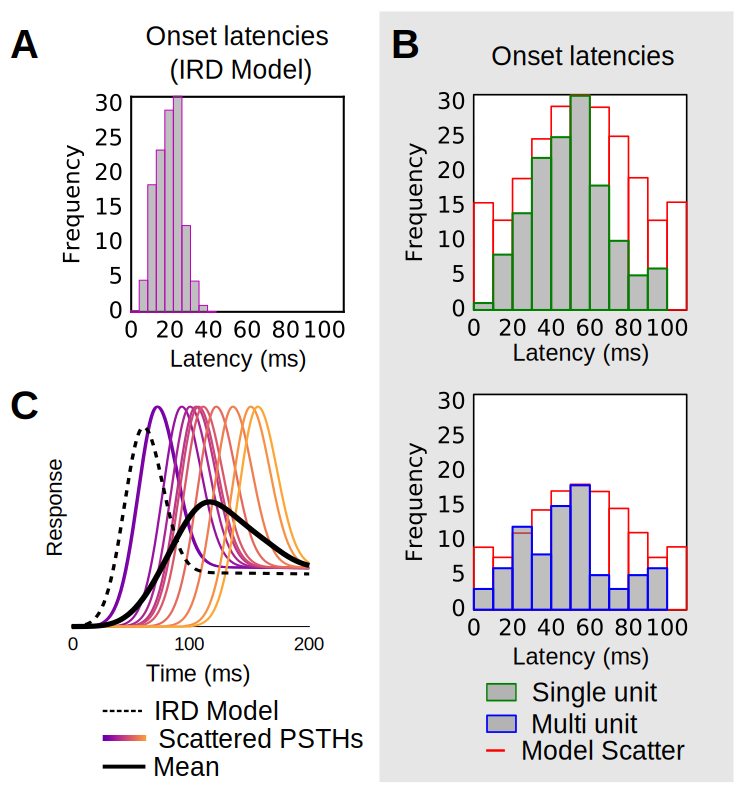
\includegraphics[width=0.7\textwidth]{./figures/sird_calibration_latency_scatter_curves.pdf}
\caption{{\bf Calibrated latency scatter across a population of IRD PSTH
    profiles.}  (A) Onset latency scatter sampled from $1000$ PSTH
  profiles generated with the IRD model, where onset is defined as the
  time to $10\%$ peak height. Profiles were generated by assuming all
  parameters of the IRD model are normally distributed with the means
  and standard deviations given in section \ref{section:IRD_background}.
  (B) Experimentally recorded onset latency scatter distributions in
  macaque V1 \citep{nowak_visneuro95} are much broader. This analysis
  shows that it is not possible to generate realistic diversity from
  the IRD model using normally distributed parameters, presumably in
  part because the actual distributions are highly non-normal.
  Comparison shows zero-aligned single-unit (green) and
  multi-unit (blue) zero-aligned distributions.  Red histogram outline
  shows the Gaussian latency distribution profile used later in the
  model. Heights of model latency histograms normalized to the maximum
  frequency of the corresponding experimental plot. (C) Mean response
  (solid black line) of a population of $100$ IRD PSTH profiles after
  the application of the calibrated scatter. Ten randomly sampled
  profiles from this population are shown, indicated by the color
  gradient. The template IRD curve ($100\%$ contrast) without latency
  scatter is shown by the dashed black line.  Grey background indicates
  experimental data, a convention used throughout this chapter whenever
  model and experimental data are shown together.  }
\label{fig:sird_calibration_latency_scatter}
\end{figure}


There is a marked difference in the inferred IRD latency distribution
and directly recorded distributions, demonstrating that a diversity
of profiles cannot be generated from the IRD model parameters in this
way. The reason for the mismatch is that a core assumption in the
inference process is invalid. The parameters of the IRD model are
\emph{not} normally distributed, which is quickly established by
comparing the mean parameter values and their standard deviations with
their corresponding median values, also given in
\citet{albrecht_jneurophys02} and section
\ref{section:IRD_background}. Of the ten parameter values of the IRD
model, only one of these, $s_{50}$, has a median that falls within a
standard deviation of the mean, whereas normally distributed data will
have medians close in value to the means.

As the parameters of the IRD distribution cannot be assumed to be
Gaussian, their distribution profiles are only weakly constrained by the values
supplied with the IRD model. As a result, the diversity of IRD
responses will need to calibrated using data from a different experimental
source. In our initial work, we will use the experimental data that
has already been shown in Figure
\ref{fig:sird_calibration_latency_scatter}B, i.e. the observed
distribution of onset latencies.

The two latency distributions shown in B are obtained by directly
recording latency onset distributions, using the same microelectrode
to compute single- and multi-unit distributions. This data from
\citet{nowak_visneuro95} is a suitable match for calibrating the latency
scatter of IRD model units as (1) it also is recorded in macaque V1 (2)
it also represents the responses of neurons responding to an oriented
stimulus centered on the cell's receptive field. Specifically, both
studies varied spatial frequency, orientation, and retinal position of
the stimulus until the response of the neuron was maximized, and then
measured the onset latency.

Both the directly recorded latency distributions shown in Figure
\ref{fig:sird_calibration_latency_scatter}B \emph{are} approximately
Gaussian, but onset latency is not directly parameterized in the IRD
model, and the actual parameters are non-normal. To model the latency
scatter explicitly, samples are drawn from a
Gaussian distribution, resulting in the distribution profile indicated
by the red histograms. This distribution is made to be symmetric with
some additional weight in the first and last bins. This is because
latencies must be positive, requiring some redistribution of probability
mass. In addition, the chosen distribution is slightly wider than
suggested by the data in order to (1) acknowledge that any finite experimental
sampling is likely to under-represent the true width of the latency
distribution in V1 (2) as we shall see shortly, latency scatter is
\emph{not} sufficient to explain the VSDI signal and this is most
clearly demonstrated by using a plausible level of scatter that is
slightly highly than what is experimentally observed (to guard against
issues like (1) obscuring the results).

To do this, we will apply the chosen scatter distribution to a
population of IRD profiles generated at $100\%$ contrast, shown in
Figure \ref{fig:sird_calibration_latency_scatter}C. All the profiles
have the same shape and are simply shifted relative to each other by the
latency scatter, representing a localized group of neurons that are
responding in a similar way but have different absolute onset
times. When averaged, these responses do have a higher time constant, as
indicated by the solid black line. The template IRD profile without any
application of scatter is shown by the dashed black line.

The relative onset distributions shown so far begin at zero, to indicate
that causal processes require positive latencies. The issue with this
formulation, after scatter is applied, a typical PSTH shown in Figure
\ref{fig:sird_calibration_latency_scatter}C has an additional shift
relative to what is predicted by the IRD model, shown by the dashed
black line. To correct for this effect, we need to look at the
\emph{absolute} latency distribution which is also given in
\citet{nowak_visneuro95} and shown in Figure \ref{fig:nowak_data}.

\begin{figure}
\center
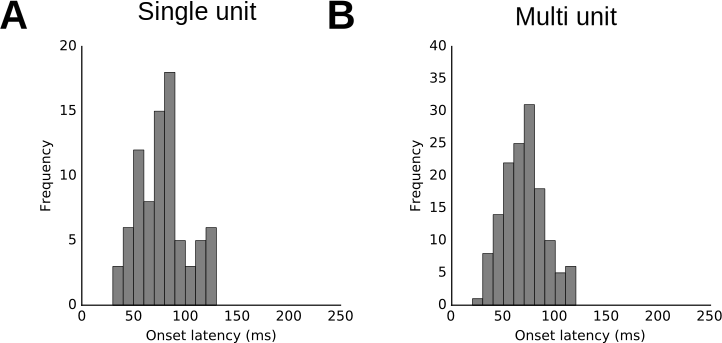
\includegraphics[width=0.7\textwidth]{./figures/nowak_data.pdf}
\caption{{\bf Distribution in onset latency evoked by the onset of a
    flashed rectangular spot of light in macaque V1.} (A) Distribution
  of onset latencies in spiking activity recorded using single-unit
  recordings (B) Distribution of onset latencies in spiking activity
  recorded as multi-unit activity. Onset was computed from the PSTH
  histogram by finding the bin at which the Poisson $P=0.01$ level was
  crossed, provided the next bin did not fall below this level and the
  following bin did not fall below the $P=0.05$ level
  \citep{maunsell_jneurophys92}. Reproduced from
  \citet{nowak_visneuro95}.}
\label{fig:nowak_data}
\end{figure}

Figure \ref{fig:nowak_data} shows how the systematic latency increase
due to the application of scatter after the IRD model profiles are
generated can be correctly compensated for. What is necessary is to
align the absolute onset latency distribution of the IRD model units
after scatter so that the distribution begins at the same absolute
latency as shown in this figure. For the single-unit data, the first bin
appears at approximately $40$ milliseconds and for the multi-unit data,
the first bin appears at around $30$ milliseconds. All the simulations
in this chapter involving latency scatter apply the necessary shift to
align with these absolute latency distributions.

What Figure \ref{fig:sird_calibration_latency_scatter}C shows is how the
time constant of a population of IRD units is increased when averaged
after the application of calibrated latency scatter. The population
response is now a closer match to the VSDI response profiles shown in
Figure \ref{fig:SIRD_comparison} than any individual single-unit
response curve. Latency scatter is therefore a promising mechanism for
increasing the time constant across a spatially extended region
\emph{without} modifying the time constant of single-unit profiles.

Note that the width of the plateau region remains narrower than in the
experimental data, which will be addressed in the final section of this
chapter. In addition, latency scatter will not be able to explain the
spatiotemporal gradient effect shown in Figure
\ref{fig:ST_gradient}D. The collection of IRD units we have been
considering have no spatial position and will therefore be unable to
account for these kinds of spatial effects.

As discussed in section \ref{section:response_across_scales}, the goal
is to identify the various forms of response diversity across a
population that are \emph{not} captured by the IRD model. Now that
latency scatter has been accounted for, we will focus on responses not
captured in the onset latencies distributions recorded by
\citet{nowak_visneuro95}. Having just noted a spatial effect at the
population level not captured by latency scatter, we will now examine
how neural responses across space. In particular, we will examine the
neural responses when the stimulus is not spatially centered on an
individual cell's receptive field, as it was in both the IRD model and
in the onset latency recordings.


\section{Dependence between space and time}

As formulated so far, the model is a collection of IRD response
profiles, each with its own variable latency. As noted in the previous
section, not only is this insufficient to fully account for the VSDI
signal at the center of the response, but it will not be able to account
for the spatial effects described in Figure \ref{fig:ST_gradient} as
there is no description of how the population of neurons are extended
spatially.

In this section, the implicit assumptions of the IRD model are examined,
focusing on what particular types of response this descriptive model may
not have captured with respect to the distance across cortical space.

\subsection{The implicit assumptions of the IRD model}

The IRD model is a descriptive model that summarizes the firing-rate
response of simple and complex cells in cat and monkey to a particular
stimulus. This stimulus is an stationary grating pattern, chosen to be
at the optimum spatial frequency, orientation, and phase for each
recorded cell, centered on the cell's receptive field.

This is to say that the measurements used to build the IRD model capture
a particular relationship that is enforced between the recorded cell and
the stimulus that drives it. This constraint reflects the decisions made
by every experimenter to study a subset of all the possible
neural mechanisms. It is simply impossible to capture all the possible responses to
all possible visual stimuli for all the recorded cells.

When considering a population response in order to understand the VSDI
signal, it is necessary to consider how these constraints should be
relaxed in order to think about other responses in the population that
have not been adequately captured. In particular, the spatiotemporal
phenomenon observed at the population level, shown in Figure
\ref{fig:ST_gradient} indicates there must be some spatially dependent
response change that has not yet been considered.

In the population model as formulated so far, all the simulated IRD
profiles are independent and are not
assigned any particular position in the cortex. That is to say, if each
IRD unit in the population were stimulated and measured in turn, with
the appropriate changes made to the stimulus parameters between
successive trials, then the current model would be valid. In reality,
all cells respond at once, such that only a minority of cells will be
optimally driven by the particular visual stimulus presented at any
given time. Given what we know about the spatiotemporal properties of
the VSD signal, we are looking for diversity in responses across the
population that varies with space.

\subsection{Observed latency variation across space}
\label{section:non_optimal_spatial}

In the same way that the latency distribution expressed in
\citet{nowak_visneuro95} connects to the IRD model due to similarities
in stimulus protocol, it is now necessary to find a new source of data
that makes contact with these two protocols that both optimize the
stimulus for a particular recorded cell. This contact needs to be made
only at one point, as we are now interested in what happens when the
constraints imposed by this stimulus protocol are relaxed. In
particular, we want to know what happens when the stimulus is \emph{not}
optimized spatially and begins to fall outside the cell's receptive
field.

Suitable data can be found in \citet{bringuier_science99} showing how
the onset latency of the subthreshold depolarizing response changes as a
function of the eccentricity of the stimulus from the receptive-field
center, for two different stimulus protocols. One type of stimulus used
was a square patch whose location with respect to the receptive-field
center is varied over two dimensions. The other stimulus was a long bar
that is varied over the direction orthogonal to its orientation. The
change in latency of the response as a function eccentricity for both
these protocols is shown in Figure \ref{fig:bringuier_data} where the
response onsets were determined using intracellular recordings in cat
primary visual cortex.


\begin{figure}
\center
\includegraphics[width=1.0\textwidth]{./figures/bringuier_data.pdf}
\caption{{\bf Latency change in subthreshold depolarizing response as
    the stimulus moves away from the receptive-field center in cat V1.}
  (A) Relative latency as a function of eccentricity for a square,
  impulse-like input ($0.4^\circ \times 0.4^\circ$) that varied in two
  dimensions relative to the center of its receptive field (n=37) (B)
  Relative latency as a function of eccentricity for a long flashing bar
  ($0.9^\circ \times 3.9^\circ$) whose position is varied over the
  direction orthogonal to its orientation.  (C) Estimate of the apparent
  horizontal velocity based on the data shown in A and B. The mode
  appears around $0.1$ \si{mm.ms^{-1}}. The latency clearly varies
  depending on the stimulus location relative to a cell's receptive
  field, with widely varying levels of spatial dependence.  Reproduced
  from \citet{bringuier_science99}.}
\label{fig:bringuier_data}
\end{figure}


There is a clear connection between this stimulus protocol using the
rectangular bar and the stimulus protocols we have been considering at
eccentricity zero. Only at this eccentricity is an oriented bar presented at
the center of the recorded cell's receptive field, in the same way it
was for both the IRD model and for the scattered recorded by
\citet{nowak_visneuro95}. Using this data, we can now observe how the
latency changes when the eccentricity varies away from zero.

What can be seen in Figure \ref{fig:bringuier_data}B is that there is a
spatially dependent latency shift as the eccentricity of the stimulus
changes with respect to the cell's receptive field center. This
spatiotemporal phenomenon is a clear candidate mechanism for explaining
the spatiotemporal gradients in Figure \ref{fig:ST_gradient}B. It is
important to note that as only relative latencies are shown, these
spatially dependent latency changes are independent of the latency
scatter that has already been introduced, i.e., additive on top of the
zero-eccentricity scatter characterized by the IRD model.

The goal is now to incorporate this spatially dependent latency shift to
our population of scattered IRD units. As the current population of IRD
units do not have an assigned spatial position, it will be necessary to
build a spatial extension of the IRD model. This introduces the
spatially extended IRD (SIRD) model that will be used throughout the
rest of this chapter.

Before switching to modeling considerations, it is worth noting that the
exact nature of the spatial latency dependence is difficult to determine
exactly due to the large spread between the cells recorded. This wide
spread is present in \ref{fig:bringuier_data}B but it is even more
pronounced in Figure \ref{fig:bringuier_data}A where a square stimulus
was used. This is a clear example of how a different feature, namely a
different stimulus shape can impact the spread of onset latencies.

Lastly, it is worth mentioning the hypothesis put forward by
\citet{bringuier_science99} to explain this effect.  It is proposed that
the spatial latency shift occurs as the dominant contribution to the
response shifts from an afferent drive when the stimulus is centered on
the receptive field to slower lateral intracortical interactions when
the stimulus moves out of the classical receptive field. This suggestion
is discussed later in section \ref{section:laminar_organization} when we
try to interpret the SIRD model but for now, we will continue to
calibrate the model in a way that is agnostic to the underlying
mechanism.

\subsection{A spatial extension of the IRD model}
\label{section:spatial_extension_SIRD}

The model now needs to be updated to incorporate this second form of
response diversity. This will be achieved in two stages. First, one
equation of the IRD model will be modified to accommodate a
distance-dependent term. Secondly, the IRD profiles will be assigned a
cortical position in order to enable a spatiotemporal analysis to allow
comparison with the experimental data. These two changes, in addition to
the latency scatter constitute the core of the spatially extended IRD
(SIRD) model.

\subsubsection*{A distance-dependent latency equation}
\label{section:distance_dependent_extension}

The first step is to identify the most appropriate place in the IRD
model that would allow a dependence between spatial position and latency
to be modeled, in order to account for the phenomenon shown in Figure
\ref{fig:bringuier_data}. The most suitable equation to extend is
exactly where the PSTH latency is computed. In the IRD model, a latency
shift is computed as a function of contrast, $\tau_c(c)$ as shown in
Equation \ref{eq:IRD_latency}.

The issue of contrast-dependent latency shifts has been ignored until
now, even though characterizing contrast responses was central to the
IRD model itself. This omission is
deliberate, allowing us to simplify the analysis of the core mechanisms of the
SIRD model. Coupling between response onset latency and contrast will be
the last mechanism to be (re)introduced to the SIRD model.

For this reason, the $\tau_c(c)$ term of the IRD model may be replaced
by a fixed value of $60$ milliseconds for the time being, corresponding
to Equation \ref{eq:IRD_latency} evaluated at $100\%$ contrast. What is
relevant to this section, is that $\tau_c(c)$ can be generalized to form
a function of both contrast and spatial distance, namely
$\tau_{cd}(c,d)$ as the sum of two independent components:
%%
\begin{equation}
\label{eq:IRD_latency_cd}
\tau_{cd}(c,d) = \tau_c(c) + \tau_d(d)
\end{equation}
%%
Here $\tau_c(c)$ is unmodified from Equation \ref{eq:IRD_latency}
although we are considering a fixed value of $c$, disabling the
contrast dependence. The fixed value of $c$ of $100\%$ contrast may be
thought of a meta parameter that has no bearing on any of the results
discussed in this chapter, until variation in $c$ is re-enabled. The key
point is that a distance-dependent latency term, $\tau_d(d)$ has been
introduced that is independent of contrast.


We will consider several possible versions of $\tau_d(d)$, starting with
the absolute simplest, linear formulation, $\tau_{d1}(d)$:
%%
\begin{equation}
\label{eq:IRD_latency_lateral_term}
\tau_{d1}(d) =  d \sigma_L + \tau_L
\end{equation}
%%
To make this equation even simpler, we will fix $\tau_L$ to zero for
now, reducing the new term to $\tau_{d1}(d) = d \sigma_L$. The variable
$d$ is the radial distance from the particular SIRD model unit (once the
units are assigned a spatial position) to the unit at the center of the
response. The $\sigma_L$ value then expresses the strength of the
spatial latency dependence.

As already noted, the exact form of the distance-latency dependence
shown in Figure \ref{fig:bringuier_data} is difficult to establish from
the data. A linear relationship is the simplest first approximation
although a gradient still required to set the value for $\sigma_L$.

Even if there were no variation in the response of all 21 cells recorded
in Figure \ref{fig:bringuier_data}B, finding a suitable value for
$\sigma_L$ would still be difficult for two reasons: (1) this
experimental data is expressed in terms of eccentricity, and the spatial
scale we have for the VSDI response shown in Figure
\ref{fig:ST_gradient}A is expressed in millimeters, and (2) this data is
recorded in cat and not macaque, making the appropriate relationship
between spatial scales even more complicated.

This data is therefore useful to show the spatial-latency effect and to
give some idea of the appropriate magnitude of the phenomenon.  The
values of $\sigma_L$ we will be considering are $0$, $35$ and $80$
\si{ms.mm^{-1}}. These odd units (reciprocal speed) are convenient with
reference to Figure \ref{fig:bringuier_data}, helps ensure the
expression in Equation \ref{eq:IRD_latency_lateral_term} is in a
particularly simple form, and allows this constant to be expressed in
terms of millisecond integers instead of with awkward floating point
values.

Looking at Figure \ref{fig:bringuier_data} the value of $80$
\si{ms.mm^{-1}} may still appear rather high (i.e., corresponding to a
very slow spatial propagation) even with the difficulties in
interpreting this value in mind. Let us assume that apparent lateral
propagation speed in macaque match those of cat. Figure
\ref{fig:bringuier_data}C shows that the mode value of the speed based
on the data shown in Figure \ref{fig:bringuier_data}B is around $0.1$
\si{mm.ms^{-1}}.  Then $\sigma_L=80 \si{ms.mm^{-1}}$ corresponds to
$\frac{1}{80}$ \si{mm.ms^{-1}} which is $8$ times too slow. An
explanation for why this value of $\sigma_L$ is still not unreasonable,
is given in section \ref{section:laminar_organization}.

Note that the additive constant $\tau_L$ may be used to express an
additional delay in milliseconds that is currently set to zero. When
$\tau_L$ is zero in this way, the central unit is a pure IRD unit that
only has an offset due to latency scatter as $d=0$ at the response
center. This unit experiences no distance-dependent latency change.

In order to examine the effect of introducing $\tau_{d}(d)$ to the
IRD model in the creation of the SIRD model, it is necessary to assign
the IRD units a spatial position in order to enable the appropriate
spatiotemporal analysis with respect to the VSD signal. This is the
topic of the next section, after which it shown that this $\tau_{d1}(d)$
term, together with latency scatter, can begin to explain the
spatiotemporal properties of the VSD signal.

\subsubsection*{A spatially sampling distribution of IRD units}

In order to simulate the effect of $\tau_d(d)$, it is necessary to move
from an unordered collection of IRD units to a model that explicitly
incorporates the spatial extent of the neural population. The goal is to
introduce a spatial component to the population of PSTH profiles in the
simplest way possible that allows the current latency scatter mechanism
to be combined with calibrated spatially dependent latency shift. In
this section, both $\sigma_L$ and $\tau_L$ of Equation
\ref{eq:IRD_latency_lateral_term} are zero, ignoring the new
spatially dependent term in the IRD model.

This can be achieved by arranging the unordered collection of IRD units
we have considered into a two dimensional array and scaling the response
amplitudes to match the approximately Gaussian profile observed in V1 as
shown in \ref{fig:ST_gradient}A. All the simulations in the rest of this
chapter make use of a regular spatial sampling of IRD units designed to
approximate the cortical response over the same spatial scale as shown
in \ref{fig:ST_gradient}A, with the response maximum located at the
center of this array. The Gaussian profile used is shown in Figure
\ref{fig:SIRD_calibration_sampling}A and its impact on the rescaled
PSTHs is shown for a regularly space subset of units shown in Figure
\ref{fig:SIRD_calibration_sampling}B.

% jbednar: Shouldn't D with scatter have the same mean latency as D
% without?  Here the scatter is shifting the onset dramatically (and confusingly).
\begin{figure}
\center
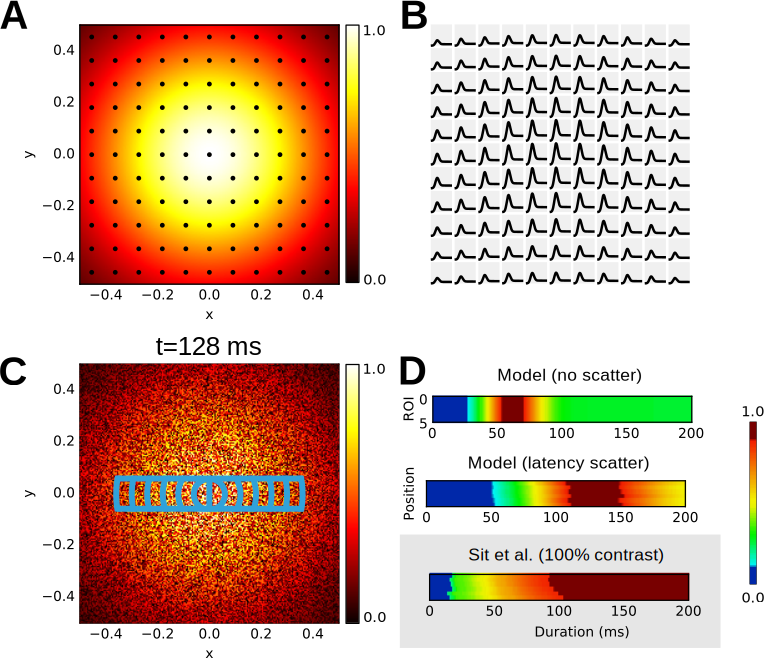
\includegraphics[width=0.8\textwidth]{./figures/SIRD_calibration_sampling.pdf}
\caption{{\bf Simple sampling grid of IRD model across cortical space.}
  (A) Gaussian profile used to scale the IRD unit responses across
  space, shown at the point of maximum response. Black points indicate
  the sample positions that scale the responses in B, drawn from the
  underlying $500\times500$ sampling grid used throughout this
  chapter. (B) PSTH profiles generated by the IRD model that are now
  given an explicit spatial positions in the cortex. Note that all these
  units have identical latencies as the response is scaled after the IRD
  model has generated a $100\%$ contrast profile, a restriction that is
  relaxed at the end of the chapter. (C) Regions of interest used to
  analyze the spatiotemporal dynamics of the response following the
  protocol used in \citet{sit_neuron09}. The ROIs are overlaid on top of
  the peak mean model response after the application of latency
  scatter. (D) Spatiotemporal plots showing the model response (top)
  shown in (A), the scattered model response shown in (B) and the
  experimental data reproduced from \citet{sit_neuron09} (bottom),
  showing the spatiotemporal logistic fits for the 100\% contrast
  condition.  These modeling results are a straightforward spatial
  extension of those already presented in Figure
  \ref{fig:sird_calibration_latency_scatter} as there is no systematic
  latency variation across space.  }
\label{fig:SIRD_calibration_sampling}
\end{figure}


As already discussed, the IRD responses are generated using a fixed
$100\%$ contrast input before they are rescaled by the spatial Gaussian
pattern shown in Figure \ref{fig:SIRD_calibration_sampling}A. The goal
is to enable the same type of spatiotemporal analysis as shown in Figure
\ref{fig:ST_gradient}A by roughly matching the spatial Gaussian profile
to the position and size of the regions of interest used by
\citet{sit_neuron09}. The scale bar in Figure \ref{fig:ST_gradient}A
will be used to determine the size of the simulated cortical area in
millimeters which will impact the value of the spatial-latency constant
$\sigma_L$.

The distance $d$ per IRD unit that is supplied to Equation
\ref{eq:IRD_latency_cd} is computed as the Euclidean distance of a unit
from the center of sheet. The origin is defined at the center and the
sheet of units extends $5$ millimeters in both directions, defining a
simulated cortical area of $10\times10$ millimeters in which
$500\time500$ regularly spaced model IRD units will be simulated.

This value was primarily chosen for convenience but it is also a good
enough match to the area shown in Figure \ref{fig:ST_gradient}A which is
$8\times8$ millimeters in size. This small discrepancy is not a major
concern as there are more substantial difficulties involved in
calibrating a suitable value of the spatial latency constant as
discussed in the previous section.

With this spatial definition, the SIRD model can be analyzed using the
exact same form of spatiotemporal analysis as used in the VSD
signal. This is shown in Figure \ref{fig:SIRD_calibration_sampling}D
where the applicable regions of interest are shown in Figure
\ref{fig:SIRD_calibration_sampling}C, overlaid on top of the peak
response after scatter. This latency scatter is applied to the IRD units
in the same way as before as shown in Figure
\ref{fig:sird_calibration_latency_scatter}.

These plots in part C show the spatiotemporal analysis for the
unscattered, scattered and experimental conditions. The difference
between the top plot of Figure \ref{fig:SIRD_calibration_sampling}D and
the middle plot is exactly the difference between an individual IRD unit
and the population average.

As the effect of latency scatter is exactly the same as before, Figure
\ref{fig:SIRD_calibration_sampling} introduced no new mechanisms. What
has changed is that a spatiotemporal analysis can now be applied and
individual units have a distance $d$ defined to the center of the
response, allowing the effect of Equation
\ref{eq:IRD_latency_lateral_term} to be investigated.

\subsection{Simulating linear spatial latency dependence}

Now the SIRD model has a notion of distance, it is time to investigate
what happens when $\sigma_L$ is increase from zero, keeping
$\tau_L=0$. As was noted previously, when $\tau_L=0$, Equation
\ref{eq:IRD_latency_lateral_term} ensures the central unit is always a
pure IRD unit (with latency scatter) as $d=0$ at the center. In
addition, when $\sigma_L=0$, the distance-dependent latency term is
disabled which is why this constant will now be increased, starting at
zero.

Figure \ref{fig:sird_calibration_spatial} shows the results using
$\sigma_L$ values of $0$, $35$, and $80$ \si{ms.mm^{-1}}. As expected,
when $\sigma_L$ is zero, the response properties are unchanged.  As
$\sigma_L$ increases, a new feature emerges as revealed by the
spatiotemporal analysis as there is now a spatiotemporal gradient,
reflecting the spatial dependency introduced by this term.

\begin{figure}
  \center
  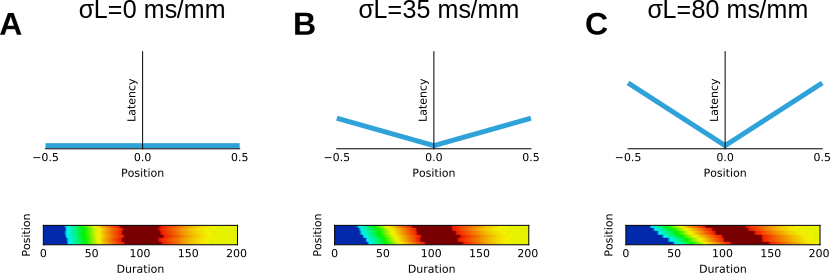
\includegraphics[width=0.9\textwidth]{./figures/sird_calibration_spatial.pdf}
\caption{{\bf Effect of changing the spatial constant $\sigma_L$ of the
    spatial latency dependence in the SIRD model defined using
    $\tau_{d1}(d)$ } (A) When $\sigma_L=0$, there is no change in
  latency as a function of position as shown in the schematic
  (top). This is exactly the same result as shown in the middle plot of
  Figure \ref{fig:SIRD_calibration_sampling}D shown zero spatiotemporal
  gradient (B) Example of a non-zero spatially dependent latency using
  $\sigma_L=35$ \si{ms.mm^{-1}}. The plot on the bottom shows that the
  spatiotemporal gradient is now non-zero. (C) Increasing $\sigma_L$ to
  $80$ \si{ms.mm^{-1}} further increases the spatiotemporal
  gradient. The qualitative effect of a non-zero spatial latency
  constant is clear, matching the non-zero spatiotemporal gradient in
  towards the end of the VSDI response seen in Figure
  \ref{fig:ST_gradient}B.}
\label{fig:sird_calibration_spatial}
\end{figure}

Although Figure \ref{fig:sird_calibration_spatial} demonstrates a
spatiotemporal dependence in the SIRD model for the first time, in some
ways we are no closer to matching the VSDI response having gained an
extra model parameter, $\sigma_L$. The reason is that we can still only
match the spatiotemporal gradient at one point in the response shown in
Figure \ref{fig:ST_gradient}B. Previously, the gradient matched at the
onset where the spatiotemporal gradient is nearly vertical and now, with
$\sigma_L$, we can still only match the gradient at only one specific
point, anywhere along the response.

This is because the VSDI signal as shown in Figure
\ref{fig:ST_gradient}B has a varying spatiotemporal gradient, starting
with a low value at point (a) and increasing towards the peak marked at
point (c). In other words, any constant spatiotemporal gradient will not
be a good match to the VSDI response. This means that the next step is
to understand why the spatiotemporal gradient shown in Figure
\ref{fig:ST_gradient}B changes over the course of the response.


\section{Diversity in latency response properties}

The first step towards matching the VSD signal was to introduce
diversity between the IRD units in the form of latency scatter. Equation
\ref{eq:IRD_latency_lateral_term} introduced a spatially dependent term
that reflects how latency changes as the stimulus moves out of a cell's
receptive field. There is still only one type of diversity in the model
as this spatial term has been applied to all the units in exactly the
same way.

This reflects another type of homogeneity across all the units in the
model: they all vary in latency as a function of space in exactly the
same way. As noted at the start of this chapter, the key to making
progress when trying to understand the population response is to
consider the different ways that neural responses may vary that are not
accounted for when starting with a single-unit model.

Having all the latency of all units depend on spatial distance from the
center of the response in exactly the same way is both unrealistic and
explains why the spatiotemporal gradients in Figure
\ref{fig:sird_calibration_spatial} are constant instead of varying. This
points to a new form of diversity, whereby all the units of the SIRD
model do not all follow the same dependence between spatial position and
latency. Note that a non-linear version of Equation
\ref{eq:IRD_latency_lateral_term} will not help, as this term only lets you
define the shape of the spatiotemporal gradient across space and will not
allow it to vary over time.

\subsection{A simple, two population model}

Having made these observations, let us try to introduce a second form of
diversity in as simple a way as possible, by introducing $\tau_{d2}(d)$:
%%
\begin{equation}
\label{eq:IRD_latency_lateral_term_2}
\tau_{d2}(d) =  \pmb{w}_i(d \sigma_L + \tau_L)
\end{equation}
%%
Here the inner term is exactly the same as before and the semantics of
all existing symbols remains unchanged. What is new is the per unit,
random variable $\pmb{w}_i$ which takes on the values $w_i=\{0,1\}$ with
some probability weighting $p$. In other words, each unit has a
probability $p$ of $w_i=0$, in which case it behaves as a pure IRD unit
and probability $1-p$ of being assigned $w_i=1$, in which case it
behaves as an IRD unit that is affected by the additional spatially
dependent latency shift. We will denote the two populations as
populations 0 and 1, according to the corresponding value of $w_i$.

This diversity means that some units of the population have a
spatial-latency dependence and others do not. We will be considering
$p=0$, $p=0.5$, and $p=1$, such that the entire population consists of
either unmodified IRD units, IRD units with a spatial latency dependence
or an even split between these two types. With no way to weight the two
populations, a $50\%$ split using $p=0.5$ is the simplest conceptual
model to consider.

Although the probabilistic component is as simple as possible, Equation
\ref{eq:IRD_latency_lateral_term_2} could be made simpler by keeping
$\tau_L=0$. A small leap will be taken that will be shortly justified by
setting $\tau_L$ to a non-zero value, specifically of $30$
milliseconds. This means that the spatially dependent units all
experience an additional, fixed delay.

Note that this possibility is \emph{not} excluded by the data in Figure
\ref{fig:bringuier_data}B as this data shows relative latency only. For
instance, it is plausible that all the cells that do not vary in latency
as a function of eccentricity have an earlier overall latency.

One possible objection is that a non-zero $\tau_L$ effectively adds an
additional spread to the latency scatter mechanism that has already been
calibrated. This would be an issue for large $\tau_L$ values but at $30$
milliseconds, $\tau_L$ is relatively small compared to the latency
spread calibrated against \citet{nowak_visneuro95}. In addition, a $30$
milliseconds is plausible according to the anatomical interpretation
presented in section \ref{section:laminar_organization}.

Figure \ref{fig:sird_calibration_two_population} shows the results of
these three different probability values, using a $\sigma_L$ of $80$
\si{ms.mm^{-1}} and $\tau_L$ of $30$ milliseconds. When $p=0$, the
results are the same as Figure \ref{fig:sird_calibration_spatial}A and
the middle plot of Figure \ref{fig:SIRD_calibration_sampling}D. When
$p=1$, the results are the same as Figure
\ref{fig:sird_calibration_spatial}C with an additional $30$ millisecond
delay. When $p=0.5$, a new qualitative property emerges, matching the
changing spatiotemporal gradient effect shown in Figure
\ref{fig:ST_gradient}B.

\begin{figure}
  \center
  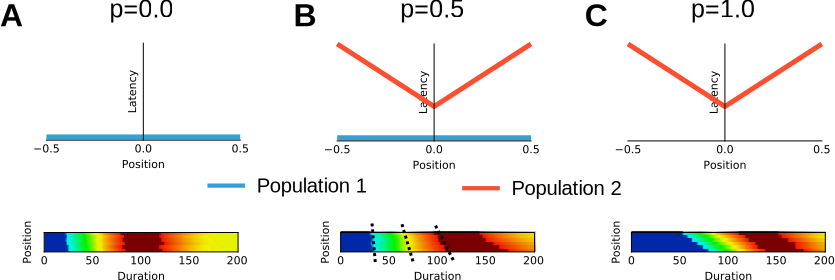
\includegraphics[width=0.9\textwidth]{./figures/sird_calibration_two_population.pdf}
\caption{{\bf Effect of probabilistic assigning units to one of two
    populations with different temporal response properties defined
    using $\tau_{d2}(d)$ } (A) When $p=0$, all units act as standard IRD
  units, as indicated by the lack of spatial dependence in the top
  schematic. There is zero spatiotemporal gradient and this plot matches
  Figure \ref{fig:sird_calibration_spatial}A and the middle plot of
  Figure \ref{fig:SIRD_calibration_sampling}D (B). When $p=0.5$, mixing
  the two types of population responses, there is a qualitative match
  with the VSDI signal as the spatiotemporal gradient increases over the
  course of the response. (C) When $p=1$ the entire population is
  delayed by $\tau_L=30$ milliseconds and all units have spatially
  dependent latencies. There is now a constant, non-zero spatiotemporal
  gradient throughout the response.}
\label{fig:sird_calibration_two_population}
\end{figure}


Why does this happen? It is important to understand the causal ordering
of the two signals and how they are reflected in the VSDI response. By
definition, the fastest cells respond earliest, and they belong to the
population that has spatially independent latencies. They will
therefore be represented most at the onset of the signal, explaining the
nearly vertical onset gradient. As time progresses, the slower cells
belonging to the second, slower population start contributing to the
response, with the cells with the lowest latency scatter appearing
first. Eventually, the response is a reflection of the \emph{averaged}
response across \emph{both} populations whereas the earliest onset
over-represented the fastest cells.

It is important to note that when describing populations 0 and 1, we are
referring to the population of IRD units in the SIRD model which have
different response properties, \emph{not} neural populations. The SIRD
model continues to make no commitments regarding the origin of these
different latency effects. All that is required is that there are two
types of response component, one which is fast and spatially independent
in latency and slower response that has a spatially dependent latency.

For instance, there could be one single population of neurons which has
the spatially dependent response component mediated by lateral
interactions that occur later, perhaps due to an additional synaptic
delays (e.g. single-synaptic versus multi-synaptic
responses).  I.e., afferent input would drive the onset of the
response, but the peak would not be reached until lateral input
arrives later.
%%
Alternatively, these two populations in the SIRD model
\emph{might} correspond to anatomically distinct populations, such as
cells in layer 4 vs.\ layer 2/3. This possibility
is discussed in more detail in section
\ref{section:laminar_organization}. What matters is simply that the
spatially dependent population is delayed, as will now be shown.

\subsection{The effect of the inter-population delay $\tau_L$}

Was it necessary to make $\tau_L$ non-zero? Figure
\ref{fig:sird_calibration_population_delay} shows the effect of varying
$\tau_L$ in order to show that the introduction of the $30$ millisecond
delay was a necessary step. Using the same $\sigma_L$ value of $80$
\si{ms.mm^{-1}} and a $50\%$ split between the two response types, the
spatiotemporal analysis is shown for $\tau_L$ values of $0$, $15$, and 
$30$ milliseconds. When $\tau_L$ is zero, there is a fixed
spatiotemporal gradient that is roughly half of the defined $\sigma_L$,
due to the averaging process over a split population. As $\tau_L$
increases, the change in the gradient over the course of the response
becomes more apparent.

\begin{figure}
  \center
  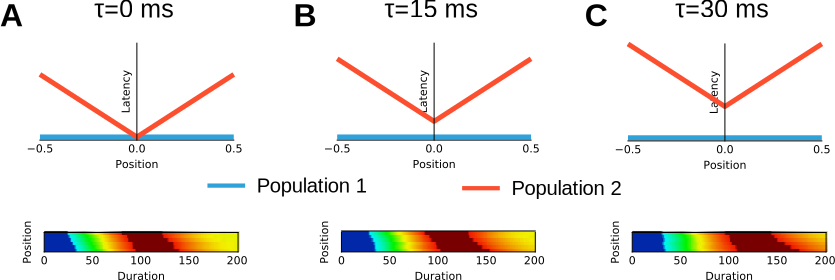
\includegraphics[width=0.9\textwidth]{./figures/sird_calibration_population_delay.pdf}
\caption{{\bf Effect of increasing the $\tau_L$ delay between the two
    randomly selected populations with equal probability defined with
    $\tau_{d2}(d)$ and a $\sigma_L$ value of $80$ } (A) When $\tau_L=0$,
  there is a constant spatiotemporal gradient that is smaller than that
  when the entire population is affected by $\sigma_L=80$
  \si{ms.mm^{-1}} as shown in
  Figure \ref{fig:sird_calibration_spatial} C. This is due to the
  averaging with the population that is not spatially dependent. (B)
  When $\tau_L=15$ milliseconds there is evidence of a gradual
  spatiotemporal increase over the course of the response (C) When
  $\tau_L=30$ milliseconds, there is a clear gradient shift over the
  course of the response as also shown in Figure
  \ref{fig:sird_calibration_two_population}B.}
\label{fig:sird_calibration_population_delay}
\end{figure}


At this point, the following aspects of the VSD response have been
accounted for (1) the increase time constant of the population response
(2) the coupling between spatial position in the cortex and latency (3)
the way this dependence between spatial position and latency changes
over the course of the response. There are still at least two things
left to explain, starting with the long plateaus in the VSD signal,
followed by the contrast-latency dependence.

\section{Diversity in tuning properties}

The SIRD model has still not accounted for all the properties of the VSD
signal, namely the way the peak response plateaus and the latency shift
with respect to different stimulus contrasts shown in Figure
\ref{fig:ST_gradient}B. As this point, two types of diversity across the
population of responses has resulted in two different, orthogonal ways
to match the VSDI response. This suggests that some other important type
of diversity has not yet been accounted for.

When the two stochastically defined populations of SIRD units was
defined, it was done with reference to the spatial-latency dependence as
captured by Equation \ref{eq:IRD_latency_lateral_term_2}. The spatial
position of a stimulus with respect to a cell's receptive field is only
one factor that might affect the response latency of a cell. In this
section, we will consider the diversity of tuning in general to capture
the relevant diversity of (nearly) everything else.

There are infinite possible features of a visual stimulus that could
affect a neuron in the primary visual cortex, including such things as
orientation, phase, spatial frequency, motion direction, motion speed,
motion energy, color, disparity, net luminance, temporal frequency, and
then the second- and higher-order statistics of all these properties
such as orientation co-occurrence and so on. In any visual experiment, a
small fraction of these features will be controlled for, and an even
smaller number will be systematically varied.

The assumption is that the uncontrolled visual features will most likely
wash out between any two experiments. Uncontrolled visual features may
be the result of much unexplained variance in neural responses, but
because these variables are uncontrolled, there is no reason to expect
systematic biases although there are no guarantees that such biases may
not accidentally occur.

This type of tuning-dependent latency variation for uncontrolled visual
features lives in an undefined, abstract and high dimensional space. It
is also already incorporated into the SIRD model via latency scatter, as
the mechanistic origin of this scatter is uncontrolled. If there was
some uncontrolled feature that explains some of this scatter, it is
reasonable to assume it was just as similar in the laboratory of Nowak
et al.\ as the laboratory of Albrecht et al. Therefore, what needs to be
accounted for specifically are the stimulus features that were not
just controlled, but explicitly optimized for each neuron recorded.

The spatial position of the stimulus with respect to the receptive field
was one such optimized parameter. The key remaining features are
orientation, spatial frequency and phase which were all optimized by
\citet{albrecht_jneurophys02} in order to evoke a clear response
from the recorded cells. To make this discussion more concrete, let us
briefly discuss orientation tuning.

Perhaps the most well-known feature about the neurons of the primary
visual cortex is that they are orientation selective. Every single
experimental protocol in all the data we have discussed so far has
worked explicitly to find the optimal orientation for a particular cell
in order to evoke a response. This is the correct approach when trying
to quantify the properties of individual cells. When considering a
population of cells, it is now necessary to account for all the cells
for which the stimulus does \emph{not} have the optimal orientation.

In macaque V1, as soon as a response spans more than one orientation
hypercolumn in cortical space, there will be a cell with every possible
orientation preference. This means that as soon as the VSD spatial
response is over a millimeter, there will be plenty of cells that are
not being driven by the orientation signal of the stimulus at all, for
\emph{any} stimulus. The key point is that it is likely that a poorly
driven cell with an orthogonal orientation preference to the stimulus is
likely to have a higher overall temporal latency.

At this point we could try to calibrate SIRD for orientation-tuning
dependent latency shifts, then spatial-frequency tuning dependent
latency shifts and so on. This is likely to be difficult, not only due
to the lack of data but because these effects are likely to be
orthogonal. The true distribution that is needed is the high dimensional
orientation--phase--spatial-preference latency distribution that is far
too high dimensional to sample effectively. For this reason, SIRD tries
to use the simplest possible distribution; the real distribution is
unknown.

\subsection{Incorporating the tuning dependent latency shift}

Two things need to be done to introduce tuning-latency diversity to the
SIRD model. First, the tuning latency shift has to be hooked up to the
IRD model and secondly, a distribution has to be chosen in the absence
of experimental data.

Now that investigation of $\tau_d(d)$ term is complete, it will be
deprecated. This is the form chosen to include the tuning dependent
latency shift $\tau_T$:
%%
\begin{equation}
\label{eq:IRD_latency_cdt}
\tau_{cd}(c,d) = \tau_c(c) + \pmb{w}_i(\tau_L + \sigma_L d  + \pmb{\tau}_T)
\end{equation}
%%
It will be assumed that whatever the $\tau_L$ delay corresponds to, it
is not specific to the spatial latency effect, now modeled by $\sigma_L
d$. It will also be assumed that the population that responds with
spatially dependent latency shifts is also the population that is
selective to the other tuning features captured by $\tau_T$. In other
words, the population with spatially dependent latency shifts are also
responsive to a diverse set of visual features.

This can be motivated by looking at the VSDI signal: whatever way we
wish to explain how peaks become plateaus, it is clear this effect is
important later in the response and is therefore a natural fit for
population 1 (the slower population that has spatially dependent
latency).

An interpretation of why $\tau_T$ only applies to this second population
is given in section \ref{section:laminar_organization}, and the SIRD
model itself continues to be agnostic towards the detailed causal
reasons for these two types of response. The two things that now need to
be justified are (1) why is $\pmb{\tau}_T$ introduced in an additive
fashion and (2) why is it not parameterized by $c$ and $d$.

Both of these points can be justified by considering the orientation
preference component of this distribution. The spread of orientation
preferences across space in macaque V1 is roughly uniform across an area
a few hypercolumns wide. The latency variation due to orientation tuning
is therefore independent of $c$ and $d$ is and should therefore be
introduced additively. This reasoning applies to the other orthogonal
features such as spatial frequency preference and phase preference.

This is why $\pmb{\tau}_T$ is unparameterized although conceptually, it
could be parameterized by $T$, representing the some abstract distance
in a high dimensional feature space. In practice this parameter is so
abstract and impossible to define concretely that it is not useful to
make this parameterization explicit.

\subsection{Modeling an unknown tuning-latency distribution}

The form of the $\pmb{\tau}_T$ distribution is entirely unconstrained by
experiment. As a result we have only two criteria (1) to use the
simplest distribution to show the effect of this term in a very general
way (2) the distribution must be positive as latencies are always
positive in a casual system.

This leads naturally to the exponential distribution, which is both
extremely simple and only defined for positive numbers:
%%
\begin{equation}
    \label{eq:SIRD_exponential}
\mathrm{Exp}(x;\frac{1}{\beta}) =
\begin{cases}
   0 & x < 0 \\ \frac{1}{\beta} \exp^{-\frac{1}{\beta} x} & x \geq 0
   \end{cases}
\end{equation}
%%
This expression can be further simplified by substituting $\lambda =
\frac{1}{\beta}$, but the form shown above is more intuitive as the
expectation (mean) of the exponential distribution is simply given by
$\beta$. Larger values of $\beta$ then correlate with a greater
variation as opposed to the $\lambda$ formulation which follows the
inverse relation.

Figure \ref{fig:sird_calibration_tauT} shows the effect of different
values of $\beta$ used in the exponential distribution used to
approximate latency variation introduced by $\pmb{\tau}_T$. The values
shown are $\beta$ when asymptotically close to zero to introduce no
variation ($\beta$ is undefined at zero), $\beta=10$ milliseconds, and
$\beta=30$ milliseconds.


\begin{figure}
  \center
  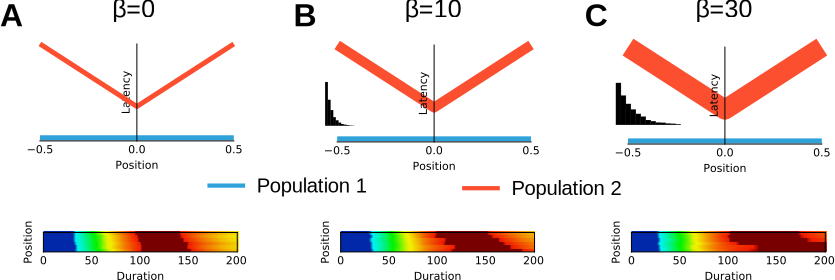
\includegraphics[width=0.9\textwidth]{./figures/sird_calibration_tauT.pdf}
\caption{{\bf Effect of increasing the $\beta$ parameter of the
    exponential distribution used to introduce latency variation via
    $\pmb{\tau}_T$ } (A) When $\beta$ is asymptotically close to zero,
  $\pmb{\tau}_T$ introduces no variation and the results are unchanged
  ($\sigma_L=80$ \si{ms.mm^{-1}}, $\tau_L=30$ ms) (B) The rust-colored
  area is extended when $\beta=10$ milliseconds (C) When $\beta=30$, the
  rust-colored area is greatly extended, showing that what was a clear
  peak is becoming a plateau, matching the VSD signal.}
\label{fig:sird_calibration_tauT}
\end{figure}

The effect of increasing $\beta$ is to increase the size of the
rust-colored region, showing the peak gradually becoming a plateau. This
is completes the demonstration that the effect of latency variation due
to $\pmb{\tau}_T$, is going to be to extend peaks into plateaus,
regardless of the details of the distribution.

The final unexplained property of the VSDI signal is already in the SIRD
model; it has simply been disabled. This is the contrast-dependent
latency shift native to the IRD model.

\section{The contrast-dependent latency shift}

All the way through this chapter, the $\tau_C$ term native to the
original IRD model was disabled as all profiles were generated as 100\%
contrast profiles in the IRD model which were them rescaled in
amplitude. This $\tau_C$ term expresses a contrast-dependent latency
shift which would have confounded the spatiotemporal analysis of the
other mechanisms in the SIRD model.

The contrast variation of a stimulus across space coupled with $\tau_C$,
the inverted Naka Rushton equation defined in Equation
\ref{eq:IRD_latency}, suggests a different type of spatial latency shift
that is contrast driven. Suppressing this effect by scaling the output
of the IRD model given a $100\%$ contrast input was necessary to avoid
conflation the two spatial latency effects.

There is another reason contrast-dependent latency shifts are
problematic. The SIRD model only models interactions within V1 and lacks
a subcortical pathway, including a retina. As contrast is only defined
at the level of the photoreceptors, the semantics of contrast become
unclear in the SIRD model. Roughly, contrast will now refer to the net
afferent drive to a cell as a result of a contrast signal. The second
problem is that it is very difficult to relate contrast scales between
experiments using different stimuli. The IRD model was calibrated using
stationary sinusoidal gratings but the VSDI data was evoked using a
Gabor stimulus.

Another problem is that the reason this effective contrast depends on
space is not clear. It could be due to actual contrast changes on the
retina, which are true for a Gabor stimulus, but it could also be
related to reduced afferent drive as the
stimulus moves out the cell's receptive field, conflating the issue with
the existing spatially dependent latency term.

With this in mind, it is time to re-enable a term that was already in
the IRD model to account for the last qualitative feature of the VSDI
onsets that requires explanation. In Figure \ref{fig:ST_gradient}B, it
can be seen that between the $100\%$ and $25\%$ conditions there is an
overall shift in response latency, a feature that cannot be explained
with the current version of the SIRD model.

Re-enabling the $\tau_C$ term offers a potential solution, as the
lower the contrast value supplied to $\tau_C$, the slower the
response. To do this, it is necessary to create a spatial pattern to act
as \emph{input} to the IRD units instead of simply scaling the response
amplitudes in the output. This spatial pattern acts like varying
contrast for the IRD model, but it can be considered the net afferent
input to each cell, rather than as the contrast of an external stimulus.

Figure \ref{fig:sird_calibration_contrast} shows the effect of
re-enabling the $\tau_c(c)$ term of the IRD model, by applying the
Gaussian spatial profile to the \emph{input} of the IRD units instead of
simply rescaling their output for the $c=100$ (percent contrast). As the
definition of contrast in this context is so nebulous, the details of
this ``effective contrast'' spatial profile are unknown. In Figure
\ref{fig:sird_calibration_contrast}A, the same Gaussian profile as shown
in Figure \ref{fig:SIRD_calibration_sampling}A is used and in B, this
spatial profile is offset by $20\%$ reducing the contrast change across
space. What is clear is that as the \emph{overall} stimulus contrast
changes, the inverted Naka-Rushton equation expressed by $\tau_c(c)$ in
Equation \ref{eq:IRD_latency} predicts that lower contrast stimuli will
have a delayed response relative to high contrast stimuli, matching what
is observed in the VSD data as shown in Figure \ref{fig:ST_gradient}B.

\begin{figure}
\center
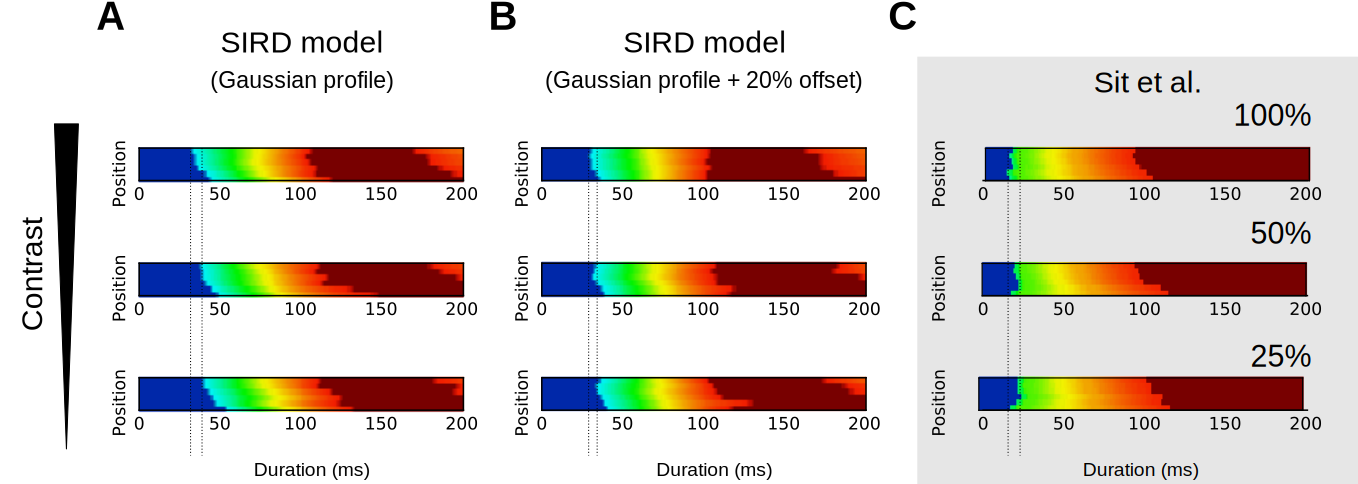
\includegraphics[width=1\textwidth]{./figures/sird_calibration_latency_contrast.pdf}
\caption{{\bf Behavior of the SIRD model as a function of stimulus
    contrast when $\tau_C$ is not locked to a $100\%$ contrast
    latency}. Response of the SIRD model as a function of contrast for
  two different spatial input profiles in relation to the experimentally
  recorded VSDI signal in macaque V1 \citet{sit_neuron09} (A) Behavior
  of the SIRD model when the Gaussian spatial profile shown in Figure
  \ref{fig:SIRD_calibration_sampling}A is used as input to drive the IRD
  units instead of using it to rescaling the $100\%$ contrast IRD
  profiles (B) Behavior of the SIRD model as a function of three
  different contrast levels when this profile is given as a fixed $20\%$
  offset. As the relative variation of the afferent drive across space
  has been reduced, the spatiotemporal gradient due to the
  contrast-dependent latency shift is decreased. No specific contrast
  values have been assigned due to the difficulties of relating
  contrasts between different experiments using different stimuli (C)
  Experimental results when using $100\%$, $50\%$, and $25\%$ contrast
  conditions in the \citet{sit_neuron09} stimulus protocol.  Note that
  the model now reproduces the main features of the VSDI imaging
  results, including the delayed peak relative to the IRD model, the
  increased spatial gradient for the peak, the wide plateau at the peak
  the increased spatial gradient at the peak compared to the onset, and
  now the longer latencies for low-contrast stimuli.  Note that these
  three experimental plots do not show the raw data, but instead present
  the best logistic function fit to the time taken to reach the $10\%,
  50\%$, and $90\%$ response levels within each ROI. Applying the
  logistic fits to the SIRD model output would further improve the match
  with the experimental data shown.}
\label{fig:sird_calibration_contrast}
\end{figure}

It is also important to note that the response amplitudes will also have
changed as they are now determined by the IRD model, which saturates at
high contrast due to Equation \ref{eq:IRD_amplitude}. These differences
are not easily visible in the spatiotemporal plots shown in Figure
\ref{fig:sird_calibration_contrast} as the trace for each ROI has been
individually normalized. At this point, the SIRD model would need a more
detailed subcortical pathway that would require the development of a
more complete mechanistic model of the visual system, starting at the
photoreceptors of the retina.  As the rest of this thesis focuses on
building such a model in general, we will not further attempt to make
the SIRD model fully mechanistic.

In any case, this final mechanism completes the account of spatiotemporal VSDI onset
response properties by demonstrating latency shifts as a function of
overall stimulus contrast. This mechanism also predicts that the VSDI
onset gradient is not vertical, in as much the effective afferent
contrast input varies across space. This spatial profile is not known
but a perfectly vertical onset gradient indicates no such
spatial-contrast-latency variation.

\section{Discussion}

The SIRD model has been formulated is a very specific way, connecting up
different forms of experimental calibration within a very simple
mathematical framework. The goal till now has been to explain the VSD
signal in terms of what is observed in a way that is as agnostic to the
detailed anatomy and mechanistic explanation.

In this section, the whole model is summarized and the interpretation of
the model is discussed. One minor, optional extension to the model is
described followed by a discussion of the limitations of the model.



\subsection{Model summary}
\label{section:model_summary}


The entire model can now be summarized by one equation where the latency
scatter distribution $\pmb{\tau}_S$ and compensation shift $k_S$ can be
folded into the definition as $(\pmb{\tau}_S - k_S)$. The original
$\tau_c(c)$ term of the original IRD model is augmented with
$\tau_{cd}(c,d)$ as follows:
%%
\begin{multline}
  \label{eq:IRD_latency_equation}
  \tau_{cd}(c,d) =
  \underbrace{\overbrace{\tau_c(c)}^{\text{IRD Model}}}_\text{Contrast shift} +
  \overbrace{(\pmb{\tau}_S - k_S)}^{\text{Latency scatter}}
  + \underbrace{\pmb{w}_i}_\text{Weighting spread} +
  (
  \overbrace{\tau_L}^{\text{Delay}}
  + \underbrace{\sigma_L d}_\text{Spatial shift}
  + \overbrace{\pmb{\tau}_T}^\text{Tuning spread}
  )
\end{multline}
%%
% k_s needs to be found properly...
The constants are $\tau_L=30\si{ms}$, $\sigma_L=80\si{ms.mm^{-1}}$, and
$k_S=30\si{ms}$. Here $\pmb{\tau}_S$ is a Gaussian
distribution, $\mathcal{N}(\mu,\sigma)$ with $\mu=60\si{ms}$ and
$\sigma=30\si{ms}$ that is clipped into the range $[0,120]\si{ms}$,
$\pmb{w}_i$ is a Bernoulli distribution, $p=0.5$ and $\pmb{\tau}_T$ is
an exponential distribution, $\mathrm{exp}(\beta)$, with $\beta=30
\si{ms}$. The only other component is the spatial Gaussian input used to
drive the $500\times500$ units over a $10\times10$ millimeter cortical
area, used to define $d$ which is the distance of the unit from the
center of the sheet.


\subsection{Lateral interactions}
\label{section:lateral_interactions}

Cortical neurons have lateral as well as afferent inputs. Lateral
connectivity and the finite speed of lateral propagation is a natural
mechanism to link the responses of cortical units across cortical space.
There are several reasons lateral connectivity may be particularly
important to understanding the VSD signal. Firstly, lateral connectivity
is more superficial and therefore more likely to be represented in the
signal. If this layer is heavily influenced by lateral interactions,
then this is likely to be reflected in the signal, either because the
neural response at the cell bodies are modulated by lateral interactions
or because the voltage sensitive dye binds to the lateral connectivity
itself.

The second reason lateral connectivity is relevant is that the VSD
signal records activity over a large cortical area and will pick up the
response from all cells, whether the response is afferent driven or
laterally driven. This consideration establishes an important link
between model definition and the VSD signal.

The hypothesis of \citet{bringuier_science99} is that peripheral
subthreshold depolarizing responses are relayed by horizontal
connections within area 17 of cat primary visual cortex. As the
eccentricity of the stimulus increases from the receptive field center,
the stimulus will eventually fall out of the classical receptive field
which means that if the cell continues to respond, it is must be driven
by the extra-classical receptive field. In this regime, lateral
interactions become particularly important and the hypothesis is that
the finite speed of lateral propagation may explain the data shown in
Figure \ref{fig:bringuier_data}. The idea is that when the stimulus is
further from the receptive field center, the cell will reach its peak
response only once lateral interactions reach it, which are relatively
slow because they need time to propagate over cortical distance.

In the VSDI signal, there is bound to be a mix of contributions from
cells driven from within their classical receptive fields as well as
from outside it. What really matters is that the vast majority of cells
in layer 2/3 will be strongly represented in the VSD signal because they
are more superficial and nearly all these cells will receive lateral
inputs, regardless of the ratio of afferent to lateral drive. Assuming
this basic hypothesis, what Figure \ref{fig:bringuier_data} then shows
is how lateral interactions affect latency across space in a way
relevant to the VSD signal.

%% Possible cite Buzas paper here
Assuming this interpretation, the spatial-dependent latency term,
$\sigma_L d$ is implicitly capturing properties related to lateral
connectivity, with the value of $\sigma_L$ being related to the average
speed of lateral propagation. If this is true, the SIRD model only
captures the coarse features of lateral connectivity which in reality is
structured and patchy.

Lastly, the lateral interactions may be involved in explaining the
$\tau_L$ constant that defines the delay between the two populations of
response. For instance, there could be an additive delay due to the
multi-synaptic nature of lateral interactions although the time
constants involved make this explanation implausible as the $\tau_L$
value used in the SIRD model is $30$ milliseconds. A more plausible
account for this delay is described in the next section, where laminar
differences are considered.

\subsection{Laminar organization}
\label{section:laminar_organization}

Structurally, the afferent cortical input generally arrives in layer 4,
and long-range lateral connectivity is mostly confined to other, more
superficial layers, such as layer 2/3. This anatomical structure
suggests a natural explanation for Equation
\ref{eq:IRD_latency_lateral_term_2} even though it was not formulated
with reference to laminar differences.

The basic idea is that the non spatially dependent response corresponds
to the earlier input layers of the cortex, starting with layer 4 where
the cortex first receives afferent input. This population of cells in
the cortex then corresponds to the fast responding population 0 of the
SIRD model.

In addition, there is little lateral connectivity in layer 4 which
explains why these afferently driven neurons all respond with similar
latencies. The more superficial cells in layer 2/3 will only receive
afferent input after a delay and these are the cells that have
horizontal connections that would explain the spatially dependent
component to the response. This would mean that population 1 of the SIRD
model corresponds to layer 2/3 cells that are not strongly driven enough
by their afferent inputs to respond immediately, and that have to wait
for laterally mediated depolarization before they start to respond.

The $30$ millisecond gap between the two populations is also plausible
in the context of this laminar explanation. Figure
\ref{fig:maunsell_laminar} shows latency as a function of cortical depth
presented in \citet{maunsell_jneurophys92}. This figure shows that a
$30$ millisecond spread between the geniculate-recipient layers and the
superficial layers is reasonable.


\begin{figure}
  \center
  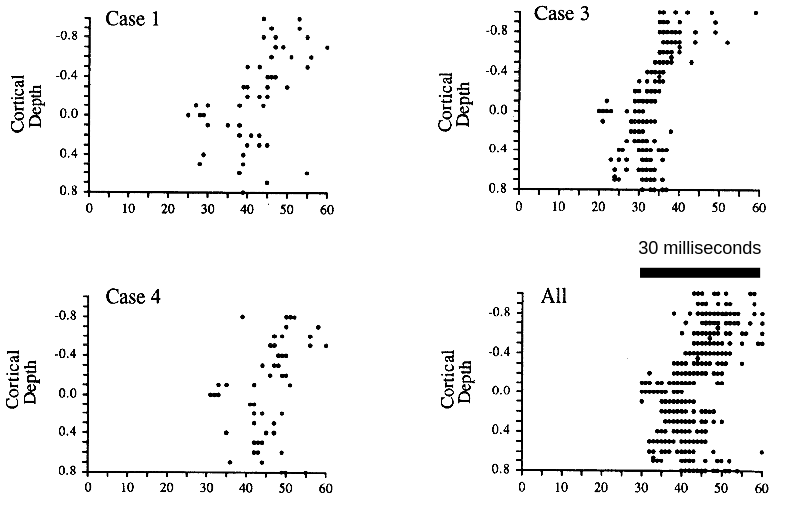
\includegraphics[width=0.9\textwidth]{./figures/maunsell_laminar.pdf}
\caption{{\bf Scatter plots of latency as a function of cortical depth in
    macaque V1 showing multiunit recordings in three cases}. Zero depth
  was physiologically determined layer 4C and negative values indicate
  more superficial layers. The condition marked ``All'' combines the three
  cases by aligning the earliest latency observed in each animal with
  $30$ milliseconds. As expected, shortest latencies are in the
  geniculate-recipient layers and latencies become longer as cortical
  depth decreases.  Additional scale bar shows that a $\tau_L$ value of
  $30$ milliseconds is plausible given these results. Data reproduced
  from Figure 12 of \citet{maunsell_jneurophys92}.}
\label{fig:maunsell_laminar}
\end{figure}


The last thing that can be explained by the laminar interpretation is
why the value of $80$ \si{ms.mm^{-1}} is so high in the SIRD model,
corresponding to a propagation speed around $8$ times slower than the
mode speed in Figure \ref{fig:bringuier_data}C. The stated $\sigma_L$
suggests it takes $80$ milliseconds to traverse one millimeter of cortex
is very slow given that the data suggests it should take around $10$
milliseconds. The key is to realize that the high value reflects the
simplified, even weighting between the two populations which in this
interpretation means both populations contribute to the signal equally.

There is in fact a tradeoff between the value of $\sigma_L$ required in
the SIRD model to account for the VSD signal and the weighting of the
two types of response, determined by the probability $p=0.5$.  This
effect was first noticed in Figure
\ref{fig:sird_calibration_population_delay}A where the spatiotemporal
gradient was observed to be decreased relative to the response for the
same $\sigma_L$ value ($80 \si{ms.mm^{-1}}$) when it was applied to the
entire population. In other words, increasing the weighting given to the
non-spatially dependent population reduces the spatiotemporal gradient
for any chosen value of $\sigma_L$.

Given a lack of information about how strongly the two populations are
represented, a value of $p=0.5$ is used, weighting both populations
equally. In the laminar account of the model, it is clear that the fast,
spatially independent population should be weighted far \emph{more}
heavily than the slower population, allowing for a lower, more realistic
value of $\sigma_L$. This is because layer 4 is not only deeper, making
it more difficult for the photonic signal to emerge from the tissue, but
also because less voltage-sensitive dye will be unable to bind to very
deep cells.

This fact that in the SIRD model, splitting the population of units in
two halves the spatiotemporal gradient suggests that to achieve a
suitable spatiotemporal gradient, the equation $\sigma_L \times p = 40$
needs to be satisfied, which means the approximate biophysical value for
lateral propagation in the SIRD model is $\sigma_L=40$
\si{ms.mm^{-1}}. This is closer to the mode value, as shown by the speed
value of $\sigma_L=10$ \si{ms.mm^{-1}} in Figure
\ref{fig:bringuier_data}C but this still is not weighted correctly. The
SIRD model has a very simple averaging process that ignored many
important details. In reality cortical cells are not perfectly segregated
into two neat layers, there are many intermediate cells, there is a
variable signal loss as a function of depth depending on how well
photons can exit the tissue, less voltage sensitive dye will bind to
deeper layers and so on.

The last thing the laminar account can explain is why the effect of
$\pmb{\tau}_T$ is applied to the second population only. Firstly, any
effect that occurs in the second population will be more strongly
represented in the VSD signal if the correspond cells are in a more
superficial layer.  Secondly, $\pmb{\tau}_T$ will be a more important
term for neurons that are selective, i.e., that have narrower tuning
curves. There is some evidence that neurons of layer 4 are less
selective than those of layer 2/3, at least where orientation
selectivity is concerned
\citep{ringach_jn02,gur_cerebral05,snodderly_jneurophys95}.

Additionally, the ``All'' case of Figure \ref{fig:maunsell_laminar}
indicates that the latency spread in the more superficial layers is
greater than at cortical depth zero which corresponds to layer 4C. This
matches the idea that there is additional, tuning-dependent latency
variation in the second population of the SIRD model and that this
population corresponds to layer 2/3.

In conclusion, the laminar account may be able to explain several
features of the SIRD model (1) the reason for the delay between the two
populations (2) that the value of this delay is reasonable (2) why it is
the slower population that is associated with the spatially dependent
latency shift (3) why the $\sigma_L$ value needed to match the VSD
response does not correspond directly to lateral propagation speed and
that a high $\sigma_L$ value is reasonable (4) why the $\pmb{\tau}_T$
distribution is applied to the slower population.

\subsection{Photonic Scatter}
\label{section:photonic_scatter}

One other mechanism was tested and calibrated for SIRD, and it does
make the simulated response slightly more realistic, but it was not of
sufficient value to include in the final model. This mechanism is
photonic scatter, implemented as a simple Gaussian blurring step
applied to the sheet of units.

What photonic scatter is designed to simulate is the spatial blurring of
the signal as the photons exit the neural tissue. This smoothes out the
spatial response profile and helps eliminate the spatial noise effect
that results from latency scatter as seen in Figure
\ref{fig:SIRD_calibration_sampling}C. If photonic scatter had been
applied, \ref{fig:SIRD_calibration_sampling}C would have been smoothed
out to look more like Figure \ref{fig:ST_gradient}A.

It is worth emphasizing that the noisy appearance of Figure
\ref{fig:ST_gradient}A is only visible as a consequence of the
low-density spatial sampling we are using, and is not something that
would appear in either a high density SIRD model or in the real
experimental signal. In a population of real cortical neurons, the
spatial response profile would be smooth due to the latency scatter of
inputs across cortical depth as well as the high spatial density of
cells in the neural tissue, even without the introduction of photonic
scatter.

Unlike the latency scatter, the spatial blurring when the photonic
scattering mechanism was added smooths the signal as a smooth Gaussian
kernel was used. Knowing the spatial scale of the $10\times10$ SIRD
model sheet, it was straightforward to find the appropriate kernel size,
knowing that the blur is approximately $200 \si{\micro m}$ in size
\citep{orbach_jn83}.

Although the photonic scatter smoothed the spatial signal, it only
smoothed the spatiotemporal plots a little, by spreading response signal
between the ROIs. As these plots were the main tool used in the analysis
of the SIRD model, it was decided that although the photonic scatter
works and helps smooth the signal a little, it was not worth introducing
as another mechanism to the model.

\subsection{Computational cost of the model}
\label{section:SIRD_computational cost}

At a density of $500\time500$ there are $250000$ IRD units in the SIRD
model simulations shown. Each unit samples the IRD model at a particular
position in order to simulate a $200$ millisecond response.

Even though a simple IRD profile takes around $2.5$ milliseconds to
compute, it requires around $10$ minutes to generate a quarter of a
million PSTH profiles. Once the various random distributions are also
introduced to the SIRD model, there is also a lot of random number
generation involved which is also computationally expensive.

As a result, it takes around $15$ minutes to run a SIRD simulation and
analyze and visualize the output using the HoloViews tool described in
Chapter \ref{chapter:reproducible_workflow}. If faster performance were
required, there is certainly plenty of scope for aggressive performance
optimization and numerical vectorization. What is clear is that the
computational cost of an equivalent spiking simulation would be much
higher, and quite possible prohibitive.

\subsection{Limitations}
\label{section:limitations}

In this section, the limitations of the SIRD model are
acknowledged. Some of these limitations are useful pointers to future
work that could be done based on the SIRD model.

\subsubsection*{Fixed firing rate profile shapes}
\label{section:firing_rate_limitations}

One of the most obvious limitations of the SIRD model may also be seen
as one of its most surprising strengths. The VSDI signal is a very
indirect signal of population activity but the voltage sensitive dye
itself serves to reflect membrane voltage, not firing rates.

%% If anything, I believe membrane voltage is smoother! Need citations
In this sense, it is perhaps surprising that the SIRD model can get
approximate VSD signal onsets using plausible biophysical parameters
while only considering the firing rates of the IRD model. This may
reflect the fact that it is the structure of the tissue, in terms of
laminar organization and the various causal delays between signals that
are dominates the population response and not the difference between
spiking activity and membrane voltage.

The main use of the IRD model is to supply the response shapes, defined
by Equation \ref{eq:IRD_half_gaussians}) and then to scale the response
as a function of contrast. It is possible that the equations of the IRD
model, namely the Naka Rushton equation for response saturation and the
inverted Naka Rushton equation for the contrast-dependent latency shift
would be just as applicable to a the membrane voltage template instead
of a firing rate template.

Perhaps the main reason the SIRD model works is because all the
mechanisms introduced apply to membrane voltages as well as firing
rates. The spatially dependent latency shift used membrane voltage
recordings directly, so at least this mechanism is appropriate, even
though the data was obtained in cat and not macaque.

The concept of latency scatter is applicable when considering the
membrane voltage, as is the idea that the diversity of tuning may impact
latency. The form of the equations as well as the laminar explanation
are also applicable whether membrane voltage or firing rates are
considered.

A more important problem with the SIRD model may be that the shape of
the response is based on the IRD model that applies for optimal stimuli.
Many of the latency shifts that have been introduced, including the
spatial-latency term and $\pmb{\tau}_T$ correspond to the responses to
non-optimal stimuli.  One clear way to improve the SIRD model would be
to investigate how the response template given by
\ref{eq:IRD_half_gaussians} changes when the stimulus is sub-optimal.

The firing rate representation of the SIRD model also has
advantages. Not only firing rate profiles nicely modeled buy the IRD
model for single units (and for appropriate stimuli) but they also allow
the SIRD model to connect with other firing rate models, such as
developmental map models. This is the direction taken in the next two
chapters of the thesis.

%% jbednar: discuss implications of using latency of intracellular
%% membrane potential compared to firing rate as in previous figures?

\subsubsection*{Unknown dependence on tuning}
\label{section:unknown_tauT}

Of all the parameters of the SIRD model, $\pmb{\tau}_T$ is by far the
least constrained. This simple exponential distribution served only to
indicate the qualitative effects this sort diversity has on the VSDI
signal as the true distribution of $\pmb{\tau}_T$ is unknown.

What $\pmb{\tau}_T$ represents are all the unknown dependencies between
onset latency and various visual features, namely orientation, spatial
frequency and phase. Trying to determine the appropriate form of
$\pmb{\tau}_T$ would be an interesting experimental challenge, if it is
possible to measure the properties of cells in such a high dimensional
feature space. This is suggested as future work in section
\ref{section:future_SIRD_tuning}.

\subsubsection*{Lack of detailed mechanism}
\label{section:lack_of_mechanism}

Even though the SIRD model discusses the tuning of cells, none of the
units actually have their own defined tuning properties. This is because
the SIRD model may be described as mechanistic only at the cortical
level and it lacks a subcortical pathway. In addition, a lot of the
interpretation of the model is related to laminar structure which it
lacks.

As a consequence, it would be useful to have a more mechanistic model
that can incorporate these features. A model with specific lateral
connectivity, different cortical layer, spatially structured receptive
fields and varied tuning properties across the population would be able
to account for all the components of the SIRD model is greater detail.
Some suggestions for how this could be achieved are described in the
discussion chapter in section \ref{section:future_work_laminar}.

A step towards such a model is presented in the last chapter of this
thesis by making a link from a more complete, mechanistic, and
developmental model to the SIRD model. The idea is to bring all the
calibration embodied by the SIRD model into to mechanistic
developmental, which is one of the core contributions of this thesis.

\section{Conclusion}

The SIRD model is a spatial extension of the well-validated IRD model
that is able to account for qualitative and quantitative features of the
spatiotemporal VSDI response. This extension is packed into a one line
equation that extends a single term of the IRD model that concerning
latency shifts. The key feature of the SIRD model is that it accounts
for diversity in neural responses that are often missed when recording
from single neurons with optimized stimuli, and it explains each
qualitative property of the VSD signal in terms of these different forms
of response diversity.

Although the SIRD model has a very simple mathematical definition,
justifying the form of this equation has involved many careful
calibration steps and lots of detailed discussion. It has synthesized
the data of three different single-unit experiments together into a
single framework that can explain the population response.

Even though the SIRD model does not have a subcortical pathway, all the
mechanisms have a clear mechanistic role and the equations may be
understood with reference to the anatomy. This makes it the first,
mechanistic account of the spatiotemporal properties of the VSDI signal.

Lastly, as the SIRD model is based on firing rates, it links naturally
to other firing rate models such as developmental map models. This
suggests that the origins of the various forms of diversity requires by
the SIRD model may be understood in terms of the developmental process
e.g. in terms of specific lateral connectivity.  In particular, the SIRD
model serves as a reference for the spatiotemporal developmental model
to be presented in Chapter \ref{chapter:TCAL}.

\chapter{Quantifying the dynamics of cortical development}
\label{chapter:GCAL}

The ultimate goal of this thesis is to build a mechanistic model of
visual response dynamics in the primary visual cortex. The first step
towards this goal was taken in the previous chapter, where it was shown
how the observed evoked response at the single-unit level relates to the
evoked response observed at the population level observed as recorded
with voltage-sensitive--dye imaging.

Although the spatially extended, invariant response descriptive (SIRD)
model bridges between spatial scales and across experimental techniques,
it is not a mechanistic model of the visual system. Instead, it is a
description of how the firing-rate responses of individual cortical
neurons relate to the dynamics at the population level. In order to
account for the origin of the single-unit cortical response at a
mechanistic level, it is necessary to follow afferent activity back
through to the lateral geniculate nucleus and back to image on the
retina.

Each stage of visual processing starting from the image on the retina
has a temporal response and involves the spatial integration of
activity. The neurons of the LGN have their own temporal responses
coupled with corresponding spatial responses determined by
center-surround receptive fields. Cortical neurons, have their own
spatiotemporal response, some component of which is inherited from the
dynamics of the LGN. Cortical neurons have their own diverse,
orientation-selective receptive-field structure that integrates
spatially across the LGN. The afferent dynamics of the evoked response
in V1 is a property of the entire visual system that is conveying
activity from the retina.

Each stage in the feed forward pathway is causal and the spatiotemporal
activity dynamics at each stage is a crucial factor in determining the
dynamics of the response downstream. In order to decompose the evoked
activity into its individual mechanistic components and identify each
causal contribution to the evoked response, it is necessary to trace
activity through the visual pathway, from the retina, through the LGN
and to V1.

Building a model that directly incorporates the necessary connectivity
and diversity in receptive fields throughout the early visual pathway is
a daunting task. The available connectivity data is sparse and there is
insufficient data to properly constrain the connectivity of a mature
visual system. One way to bypass these difficulties is to work with a
developmental model that starts in a simple, randomized state and that
acquires the necessary diversity in connectivity and receptive-field
structure over time.

Developmental self-organizing map models include all the key stages
required to build a mechanistic evoked response model, starting with
activity at the photoreceptor level. These developmental models have a
simple initial condition and self-organize via Hebbian learning,
developing diverse receptive-field structure that is organized into
spatially extended feature maps. Once the process of development is
complete, these models include specific lateral connectivity,
orientation selective receptive fields, contrast invariant tuning curves
and all the other essential features necessary to construct a
mechanistic, evoked response model.

There is one other, more fundamental reason why developmental timescales
are relevant to the evoked response. Only through development does
cortical structure come into correspondence with the visual
environment. In the SIRD model, firing-rate profiles were fixed but real
neurons are not static entities. The evoked response changes over time
as a function of the synaptic and network structure which is plastic and
shaped by the entire history of previous evoked responses. There is a
reciprocal connection between long and short timescales and it is this
connection that allows an evoked response to encode information about
the visual world.

In this chapter, a developmental, self-organizing map model will be
analyzed in terms of the development of orientation-selective cortical
receptive fields that are organized into smooth orientation maps. A new
map quality metric will be used to quantify the biological plausibility
of orientation map formation throughout development in order to validate
the model. This model will then form the basis of the mechanistic
spatiotemporal response model that bridges across spatial and temporal
scales within a single, consistent framework, as described in the next
chapter.

\section{Activity dynamics and development}

The SIRD model of the last chapter made use of the invariant response
descriptive model of cortical firing-rate profiles to try to understand
the voltage-sensitive--dye imaging signal. There are many possible ways
such a model could be extended, making it important to highlight the
properties of developmental map models that are particularly relevant
for understanding the properties of the evoked response.

The IRD model is a direct description of firing rate at the V1 level and
does not explicitly account for feature selectivity or the receptive
field of neurons and it does not include any details regarding the
subcortical visual pathway. Real evoked responses in the cortex are the
result of complex, mechanistic interactions as the activity propagates
from the retina to V1 via the LGN.

Any reasonably complete mechanistic account of activity in V1 needs to
start with the projection of a visual stimulus onto a simulated retina.
The retina then performs various forms of visual processing before the
activity is projected to the lateral geniculate nucleus via the retinal
ganglion cells. There, cells are observed to have ON and OFF
center-surround receptive fields which then project to cortical neurons
which typically have orientation-selective receptive fields.

A large, sophisticated compartmental model extending the SIRD model
would be able to include all of these features in great detail whereas
the developmental models we will be considering include far less
detail. The key advantage of developmental models when it comes to
understanding evoked response dynamics is their ability to address the
effect of activity-driven plasticity on long time scales alongside
receptive-field and feature map formation \citep{bednar_jpp12}.

The receptive fields of cortical neurons have been known to be
orientation selective since the work of Hubel and Wiesel over 50 years
\citep{hubel_jphysio59}. These orientation preference are smoothly
organized across the cortical surface in many primate species, as shown
by the orientation map in Figure \ref{fig:example_OR_maps}B. This
spatial, orientation preference structure is crucial to understanding
the evoked response as a receptive field represents the relationship
between some property of a visual stimulus and the neural response.

Self-organizing developmental map models demonstrate receptive-field
formation and orientation map formation, expressed in terms of activity
driven changes to synaptic strength. These changes occur very slowly and
given that receptive-field structure is an important component in
determining the evoked response, it is natural to make use of such
developmental models when trying to account for the spatiotemporal
dynamics of evoked activity across timescales. For an overview of the
self-organizing network models we will be considering, see section
\ref{section:self_organizing_networks}.

Calibrating and validating developmental self-organizing models poses
some unique challenges, most notably due to the difficulty in reasoning
about the model behavior at the end of development given only a
specification of the initial conditions and training stimuli. Although
there are many different measurements that can be performed at the end
of development, such as establishing whether or not the model exhibits
contrast-invariant orientation tuning, the most striking outcome of
the development process is an orientation preference map.

Measuring orientation preference and selectivity maps is relatively
straightforward using the standard vector averaging method
\citep{miikkulainen_2005,blasdel_nature86} whereas quantitatively
establishing the plausibility of these maps is much more
difficult. Although selectivity and stability measurements of an
orientation map are useful indicators, they are insufficient to gauge
map quality. An additional map quality metric is required which is
introduced in this chapter to evaluate the plausibility of the spatial
organization of orientation preference.

The GCAL model \citep{stevens_jn13} is the developmental model that will
be analyzed in this chapter. This model was the product of several years of
collaboration prior to me carrying out the novel map quality analysis presented
here, leading to the publication with Judith S. Law, Jan Antolik, and
James A. Bednar. The suite of metrics described in this chapter were
used to show that GCAL features realistic map development and the GCAL
publication is included in the Appendix.

\section{Evaluating orientation map quality}

An experienced neuroscientist who has inspected many different
experimentally recorded orientation maps will eventually develop a set
of subjective heuristics regarding what a smooth orientation map should
look like. In a similar way, a computational modeler who has examined
the output of developmental simulations across many different runs will
learn to judge relative stability and robustness between developmental
models. Although these types of informal heuristics are useful in the
research process, they are unsuitable for communicating results to the
wider scientific community.

In the absence of objective metrics, it is sometimes permissible to
publish a small number of results and claim that these examples are
representative of the whole. This approach tends to be problematic in
that the selection process itself is a subjective judgment that may in
turn be biased. To show that any set of supposedly representative
examples is in fact unbiased, an appropriate objective metric is once
again required.

Well-defined map metrics are therefore needed by both experimenters
and modelers, with many different measures proposed in the
literature. The way a metric is used is an important consideration, as
both experimenters and modelers may use the same metric to achieve
very different goals. An experimental scientist will typically use a
metric to summarize data recorded from a live animal. In contrast, the
aim of a computational modelers is to show that a mathematical
abstraction captures the relevant properties of the biological system
under study. Unlike the experimenter, a modeler is concerned whether
a simulated orientation map is biologically plausible.

We will start by defining selectivity and stability measures, which are
valuable, well-defined quantities, and yet we will show without an additional
measure of the map's spatial organization they cannot rigorously
constrain map quality. Existing metrics that are influenced by the
spatial arrangement of orientation preferences are then considered and
shown to impose only very weak constraints on map structure. Finally, a new
map quality metric based on $\pi$ pinwheel density is introduced which
not only imposes strong constraints on what constitutes a realistic map
but does so in a way that is species independent.

\subsection{The need for a new map quality metric}

Two of the simplest metrics for evaluating the development of simulated
orientation maps in relation to the experimental data are (1) the
average orientation selectivity and (2) the map stability index. These
two measures are now described before it is shown why they are
insufficient for assessing the plausibility of a map without also
including (3) a map quality metric.

\subsubsection*{Selectivity and stability}


The overall selectivity of an orientation map is simply the mean
selectivity across all the elements of the map, where an element may be
a pixel in an experimental recording or a computational unit in a model.
The orientation selectivity is defined using the standard vector
averaging method \citep{miikkulainen_2005,blasdel_nature86} as the
magnitude of the summed vector.

The orientation map similarity index for evaluating stability is
described in section \ref{section:ferret_map_stability}. The similarity
index ranges from zero to unity where a value of zero similarity
indicates \emph{anti}correlation and a value of one indicates a perfect
correlation. As two random maps will typically be uncorrelated, a
closely related measure is introduced called the \emph{stability index}.
This metric is a trivial rescaling of the similarity index metric such
that zero on the stability index scale indicates a lack of correlation
between maps instead of an anticorrelation.

The stability index (SI) measures how closely an orientation preference
map $O$ at a particular stage of developmental process resembles the
final available orientation map recording $F$ obtained at the end of
development. The mathematical definition is expressed as the following
sum over $n$ units indexed by $i$:
%%
\begin{equation}
  SI = 1 - \frac{4}{n \pi} \sum_{i} \left| (F_i - O_i) \mathrm{mod}
  \left( \frac{\pi}{2} \right)\right|
\end{equation}
%%
The chronic experimental recordings in ferret V1 of \citet{chapman_jn96}
show that orientation selectivity increases as the animal matures but
the map structure is stable. That is to say that the preference
organization across the cortical surface does not change after it
initially emerges, resulting in a high SI value throughout
development. These results are summarized in the Background chapter in
section \ref{section:ferret_map_stability}.

\subsubsection*{The need for a spatially sensitive metric}

Both stability and orientation selectivity are defined at the level of
individual units and map stabilities and selectivities found by
computing the average over all units. This means that these two metrics
are locally defined measures that are able to assess whether a simulated
map has suitable properties \emph{on average} but they are insensitive
to the spatial properties of the map. In other words, these measures do
not take into account the way the orientation preference might change
from one unit to the next.

This problem can be illustrated by considering the differences between a
salt-and-pepper organization typical in rodent V1, such as the one shown
in Figure \ref{fig:example_OR_maps}A with the smooth, structured
orientation maps observed in primate V1, such as the one shown in Figure
\ref{fig:example_OR_maps}B. These two types of map pattern are clearly
distinct with a salt-and-pepper arrangement highly unlikely to be found
in an adult primate and smooth map highly improbable in the
rodent. Nonetheless, selectivity and stability measures alone are unable
to distinguish between these two cases.

Mathematically, the computation of map stability and selectivity values
of a large primate orientation map is identical to any spatially
scrambled version of itself. It is clear that to properly assess
developmental models of orientation map formation, an additional metric
is needed that can take the global spatial organization of the map into
account.

\subsubsection*{Existing orientation map structure metrics}

The biological plausibility of an orientation map is not only defined by
the properties of individual units but is a function of the overall
spatial map organization. Some existing non-local measures will be
considered before the novel $\pi$ pinwheel map quality metric is
introduced.

Local smoothness is one property that could easily distinguish between
how orientation maps are spatially organized in primates from the
salt-and-pepper arrangement in rodents.  Several measures of smoothness
have been used in the literature including the ``local homogeneity
index'' \citep{nauhaus_neuron08} and the ``local input orientation
selectivity index'' \citep{schummers_jpp04}. These measures express how
rapidly orientation preference change across the cortical surface in a
small region around a particular cortical location.

Although these smoothness metrics can distinguish salt-and-pepper
organizations from primate maps, they fail to distinguish between two
maps that are equally smooth. In other words, there are many possible
maps with an unrealistic spatial organization for any given chosen of
smoothness. To illustrate, a planar sinusoidal wave pattern of
orientation preferences is a pattern that is both very smooth and
biologically implausible. Autocorrelation is a similar measure that acts
as as another smoothness criterion which is just as weak when assessing
the plausibility of map structure.

Another approach is to examine the statistical properties of population
distributions instead of averaging values across all units and reducing
the measurement to a single scalar. For instance, it has been
empirically shown that the representation of orientation preferences
across a map deviates from a perfectly uniform distribution
\citep{coppola_pnas98,muller_nc00,tanaka_plosone09}.

A simulated map with a plausible orientation distribution histogram will
be arranged such that each preference value has the appropriate overall
level of representation across the map. Although this is an important
criterion, species with smooth map organization, it is only applicable
over large cortical areas covering enough different orientation
hypercolumns to achieve an unbiased average.

Conversely, in a species with salt-and-pepper organization, the
orientation distribution histogram can take any shape once the
preferences of enough cells are collected together. Once again, this
measure cannot detect the difference between an appropriate balanced
smooth map and a salt-and-pepper arrangement although this metric can
detect when a particular orientation preference is under- or
overrepresented.

A more promising approach is to examine the spatial properties of the
orientation hypercolumns themselves. Different species have different
hypercolumns sizes and estimating the typical distance between
orientation hypercolumns is a crucial statistic for describing the
spatial organization of the map. Generating a good distance estimate
involves analyzing the spatial distribution of preferences in a way that
offers some useful insights into what constitutes a realistic map.

\section{Constructing a map quality metric}

In this section, a simple approach for estimating the hypercolumn
distance is first described, followed by a description of the pinwheel
density, and more specifically, the phenomenon of $\pi$ pinwheel
density.

The hypercolumn distance offers a natural species-dependent spatial
feature to measure, whereas pinwheel density is normalized by 
the hypercolumn distance to have a species-independent
reference value. The novel use of $\pi$ pinwheel density for assessing
orientation map simulations is discussed and the heavily tailed gamma
squashing function is then introduced.

%%\TODO{Ask Jim is there is a convention for citing supplementary material}
%% jbednar: Maybe (Kaschube 2010, fig. S2) or (Kaschube 2010,
%% supplemental fig. 2) or  (Kaschube 2010, supplementary material)?
\subsection{Estimating the hypercolumn distance}
\label{section:hypercolumn_distance}

There are several different approaches to estimate the hypercolumn
distance, $\Lambda$, based on the spatial periodicity of the orientation
preferences across the cortical surface. The simplest approach is to
examine the polar Fourier power spectrum which tends to be ring-shaped in
experimentally measured maps \citep{erwin_nc95,blasdel_jn92a}. In
Fourier space, a periodic, spatially extended signal with an isotropic
characteristic distance is mapped to a fuzzy ring, as shown by the
middle column of Figure \ref{fig:fourier_ring}.

In addition to generating an estimate from the size of the Fourier power
spectrum ring, a more advanced wavelet-based analysis technique is
sometimes used \citep{kaschube_science10}. Wavelet analysis offers an
improvement over the Fourier approach when it is necessary to account
for retinotopic anisotropy in V1 that results in a distortion of the
ring in the Fourier domain. We will focus on the Fourier approach here, as
wavelet analysis is significantly more complicated, the quantitative
difference from the Fourier approach is small, and all the simulated
maps that we will be considering are perfectly isotropic.

An example polar Fourier power spectrum of an orientation map is shown
in Figure \ref{fig:fourier_ring}B. The simplest way to find the radius
of a circular ring (i.e., for an isotropic map) is to average the power
spectrum radially to build a one dimensional histogram, as shown in the
column on the right side. Locating the tallest bin is one simple way to
estimate the ring radius but this approach ignores the information
contained in the overall shape of the distribution.

\begin{figure}
\centerline{
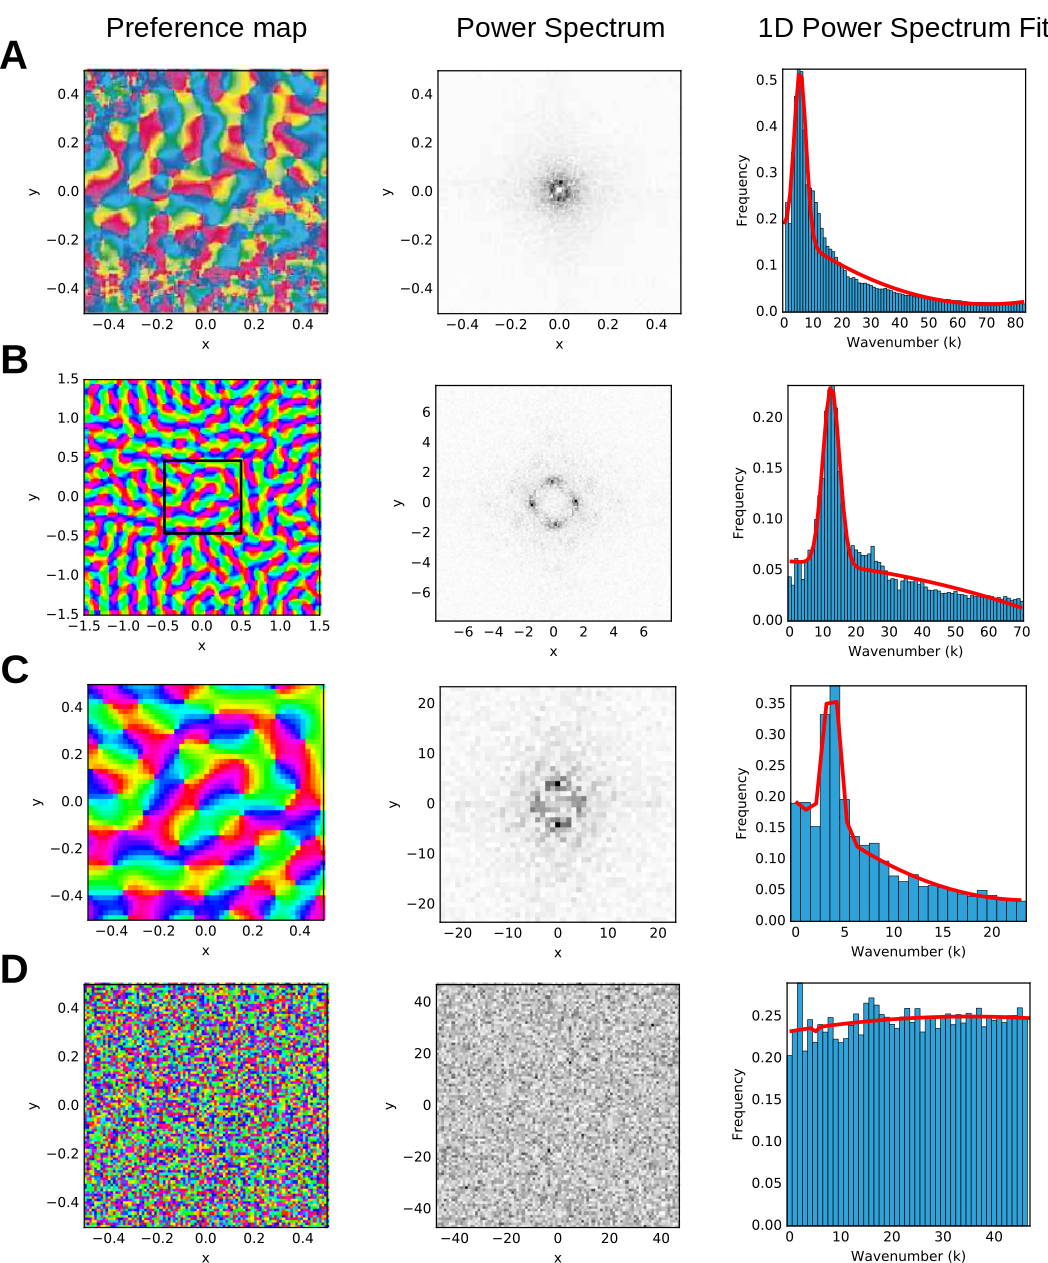
\includegraphics[width=0.8\textwidth]{./figures/fourier_rings.pdf}
}
\caption[]{{\bf Polar power spectrum analysis of a range of experimental
    and artificial orientation maps.} Left column shows orientation
  preference maps. Middle, the corresponding polar Fourier power
  spectrum. Right, the 1D power spectrum histogram (blue) together with
  the fits of Equation \ref{eq:kaschube_hypercolumn_fit} (red) used to
  estimate the hypercolumn distance following the methods of
  \citep{kaschube_science10}. (A) Ferret orientation map reproduced from
  \citet{chapman_jn96}. Note that the central $4\times4$ area of the
  polar power spectrum is set to zero to eliminate the DC component and
  better illustrate the power spectrum fit on the right.  (B) Artificial
  orientation map (GCAL model) with a larger ring in the Fourier power
  spectrum. The stronger power in the cardinal directions is an artifact
  of running a simulation on a Cartesian grid. (C) The central area of
  (B) marked in the black square. Note that with fewer samples, the ring
  is noisier but approximately the same relative size as before. This is
  because the increased spatial frequency of the hypercolumns in the
  available area is offset by the reduced number of samples necessary to
  compute the high frequency components of the image. (D) Example of a
  map generated by random noise, similar to the salt-and-pepper
  arrangement in rodents. The ring is no longer present in the polar
  power spectrum and the 1D histogram is now flat.}
\label{fig:fourier_ring}
\end{figure}

Following the approach used \citep{kaschube_science10}, an estimate of
the ring radius can be obtained from the $a_1$ coefficient computed
using a least-squares with respect to the wavenumbers ($k$) using the
following fitting function:
%%
\begin{equation}
 \label{eq:kaschube_hypercolumn_fit}
f(k) = a_0 \exp \left( \frac{(k - a_1)^2}{2a_2^2} \right) + a_3 + a_4k + a_5k^2
 \end{equation}
%%
This fitting procedure makes use of the additional information in the
ring cross section and these fits are shown by the red traces in the
right column of Figure \ref{fig:fourier_ring}. A perfectly thin ring is
impossible, as this would require an exact periodicity in all directions
at all points in the map. At the other extreme, the sort of salt-and-pepper
arrangement shown in Figure \ref{fig:fourier_ring}D will have long-range
periodicity and thus no ring structure. A plausible simulated
orientation map must therefore have a noisy ring with some finite
thickness, due to the quasi-periodic repetition of the orientation
hypercolumns.

In addition to allowing the hypercolumn distance to be estimated, the
polar Fourier power spectrum helps reveal spatial properties of the map
without uninformative phase information. Although the use of the Fourier
power spectrum help simplify the analysis, hypercolumn distance alone
does not offer an objective way to distinguish a high quality map from a
poor one. In particular, the size of the Fourier ring is species
dependent, with different species having different characteristic
hypercolumn sizes.  It may be possible to express a criterion in terms
of the tightness of the ring (i.e., how ring-shaped it is), but as we
will see in the next section such a criterion is subsumed by the
proposed $\pi$ pinwheel density metric. 


\subsection{Pinwheels and $\pi$ pinwheel density}

In addition to orientation hypercolumns, another natural spatial feature
that can be identified and quantified are the pinwheel singularities. A
pinwheel is a point in the map around which all possible orientation
preferences are represented. Pinwheels have one of two polarities,
depending on whether the orientation preference increases in the
clockwise or counterclockwise direction around it.

In smooth, well-organized primate map, pinwheels tend to be fairly
evenly distributed over the cortical surface. The spatial distribution
of pinwheels has been analyzed and it has been found that the average
distance between nearest-neighbor pinwheel pairs tends to be lower
between pinwheels with opposite polarity \citep{muller_nc00}.

Automatic identification of pinwheel locations is possible by finding
the intersection between the zero contours in the real and imaginary
components of the polar representation of orientation preference
\citep{lowel_ejn98}. Correctly identifying pinwheels in experimental
maps is non trivial, requiring a careful filtering procedure that will
be discussed shortly.

The orientation map quality metric for developmental simulations
described in the next section is based on the remarkable empirical
discovery of $\pi$ pinwheel density across carnivorans, primates, cats,
and tree shrews \citep{keil_science12,kaschube_science10}. This
observation relies on the linear relation between the size of
orientation hypercolumns across different species, and the pinwheel count
per unit area. As map size increases, the average
number of pinwheels in a unit hypercolumn area ($\Lambda^2$) tends to the
mathematical constant $\pi$. The pinwheel density, $\rho$, is simply the
number of pinwheels found on average in area $\Lambda^2$, where the
$\Lambda$ value may be computed using the Fourier power spectrum method
described in the previous section.

To support the claim that $\pi$ pinwheel density is a universal
property, \citet{kaschube_science10} analyzed hundreds of orientation
maps in three species, namely tree shrew, galago, and ferret. Figure
\ref{fig:kaschube_pi_density}A shows the linear relationship between
pinwheel count per unit area and the hypercolumn distance and Figure
\ref{fig:kaschube_pi_density}B shows that this gradient centers around
$\pi$.

\begin{figure}
\centerline{
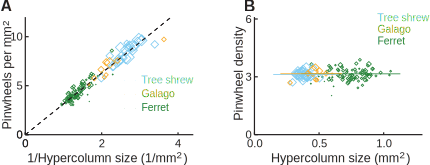
\includegraphics[scale=1]{./figures/kaschube_pi_density.pdf}
}
\caption[]{{\bf The relationship between absolute pinwheel density and
    hypercolumn size.} (A) A linear relationship between number of
  pinwheels per \si{\mm^{-1}} of cortex and the inverse hypercolumn size in
  ferret, galago, and tree shrew. (B) The gradient of this relationship
  is a unitless constant shown on the $y$ axis, with pinwheel densities
  centered on $\pi$ .  Figure reproduced from
  \citet{kaschube_science10}.}
\label{fig:kaschube_pi_density}
\end{figure}

These maps used in this analysis had to be carefully filtered, using the
methods described in the supplementary materials of
\citet{kaschube_science10}. In particular, a Fermi filter was used with
species-dependent cutoff frequency values in order to ensure the
filtering process did not mask or distort the computed pinwheel
density. For instance, Gaussian filtering does not allow an objective
definition of the pinwheel density \citep{kaschube_science10} as it
obscures the real structure of the underlying map.

The surprising empirical observation of $\pi$ pinwheel density across
species has the necessary attributes to build a suitable metric. It
defines a unique reference value that can be used to constrain
artificially generated maps in relation to experimental measurement.

The dimensionless constant of $\pi$ is not selected arbitrarily but
emerged from a theoretical analysis in terms of the universality class
of self-organizing phenomena to which orientation map formation is
thought to belong \citep{kaschube_science10}. As pinwheel density can be
computed automatically when considering simulated maps, it offers a
solid basis to build a species-independent map quality metric for use in
orientation map models.

\subsection{An orientation map quality metric for simulations}

The pinwheel densities shown in Figure \ref{fig:kaschube_pi_density}B
have been computed from experimentally recorded orientation maps which
have a small spread around the value $\pi$. To build a map quality
metric based on pinwheel density it is necessary to consider the
potential range of pinwheel densities of orientation maps that may be
generated by a simulation, from the highly implausible maps to highly
realistic ones.

As pinwheel density is simply the average number of pinwheels per
hypercolumn area, it can be any positive value. An arbitrary number of
pinwheels may reside within a hypercolumn area and the hypercolumn area
itself is also a positive and potentially unbounded quantity. It follows
that the only mathematical constraint on a pinwheel density value is
that it must be positive.

Figure \ref{fig:synthetic_pi_density} shows a few concrete examples
pinwheel densities for some simple patterns as well as the pinwheel
density for some example orientation map simulations. We see that the
synthetic maps shown have varying pinwheel densities that are easily
distinguished from $\pi$, varying between $0.3$ for the stripe pattern
and $4.0$ for the periodic tiling. The pinwheel densities for the
simulated orientation maps, in contrast, range from realistic values of
$\pi$ to very large values, with the worst simulated map example shown
with a pinwheel density of $3341$. The reason for such high potential
values when dealing with simulated maps will be discussed after a unit
metric has been established.

\begin{figure}
\centerline{
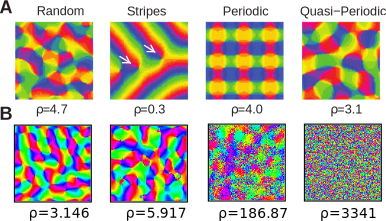
\includegraphics[width=0.8\textwidth]{./figures/synthetic_pi_density.pdf}
}
\caption[]{{\bf Example pinwheel densities for synthetic and simulated
    orientation maps.} (A) Example pinwheel densities for synthetic maps
  reproduced from \citet{kaschube_science10}.  (B) Example pinwheel
  densities for a range of simulated orientation maps of varying
  quality. We see that low quality simulated maps tend to have high
  estimated pinwheel density values.}
\label{fig:synthetic_pi_density}
\end{figure}

\subsubsection*{Normalizing the metric}

Normalized metrics that take a value between zero and one are
particularly useful, where zero denotes the worst possible metric value
and one denotes the highest possible value. Normalized metrics can be
multiplied together to create other normalized metrics and it is useful
to have a well defined upper and lower bound.

Given that pinwheel densities are positive and unbounded in principle
and the high values of pinwheel density observed in the worst
orientation preference maps shown in Figure
\ref{fig:synthetic_pi_density}, it would be useful to find a suitable
way of normalizing pinwheel density. Such a metric would have the
following six properties:

(1) The metric should vary smoothly with pinwheel density, because
functions with smooth gradients are easier to reason about. Functions
with arbitrary boundaries are more difficult to work with and are 
tricky to optimize. (2) If the pinwheel density is $\pi$, the metric should
have a value of unity, indicating a structure that is indistinguishable
from an ideal, biological map with assumed $\pi$ pinwheel density.
(3) If there are no pinwheels at all, the metric value should be zero, as a
metric based on pinwheel density is only applicable when there are
sufficient hypercolumns for a good hypercolumn distance estimate and
sufficient pinwheel singularities. (4) If there are many pinwheels and the
pinwheel density is high, the metric should tend to zero, reaching zero
at infinity. (5) Given that only pinwheel densities near $\pi$ correspond to
biologically plausible maps, the metric should converge to nearly zero
quickly, even if it only asymptotically approaches a truly zero value.
(6) Given that the modal value
$\pi$ is much closer to zero than infinity, this function will
necessarily be heavily tailed.

From these six constraints, the goal is to find a unimodal,
heavily tailed distribution. The distribution must start at the origin,
peak with unit height at $\pi$ and then rapidly fall back to zero as
pinwheel densities approach infinity. For these purposes, the gamma
distribution was chosen, as it is defined by two arguments that will be
reduced down to a single parameter.

The gamma distribution is a probability distribution that is defined as
follows:
%%
\begin{equation}
P(X=x) = \frac{1}{\Gamma(k) \theta^k} x^{k-1}\exp^\frac{-x}{\theta}
\end{equation}
%%The distribution is parameterized by $k$ and $\theta$ where $\Gamma$ is
the gamma function.  It is now necessary to find the appropriate value
of $\theta$ given $k$ to ensure that the peak always appears at $\pi$,
and then it is necessary to normalize the distribution so that this peak
value is unity.

Finding the expression for $\theta$ in terms of $k$ is straightforward
given that the mode of the distribution is expressed by $(k-1)\theta$
for values of $k$ greater than one. Constraining the desired mode value
to the value $\pi$ and rearranging yields
$\theta=\frac{\pi}{(k-1)}$. This leaves $k$ as the remaining free
parameter that is used to determine how heavily tailed the distribution
is. Finally, to normalize the metric, it is sufficient to divide the
output of this mode-constrained gamma distribution by its value at
$\pi$.

The map quality metric ($mq$) can now be expressed in terms of the
pinwheel density $\rho$ and the $k$ parameter as follows:
%%
\begin{equation}
mq(\rho; k) =  \frac{\rho^{k-1}\exp^\frac{(1-k)\rho}{\pi}}{\pi^{k-1}\exp^{(1-k)}}
\end{equation}
%%
The normalization term that was required to make gamma function into a
probability distribution cancels out in this formulation, to ensure a
value of unity at $\rho=\pi$. For a given
value of $k$, the denominator in the expression above only needs to be
evaluated once in order to obtain the appropriate normalization
constant. As shown below, the value of $k$ can be set by the modeler
to ensure that the metric is sensitive to the range of maps typically
needing to be distinguished in practice.

\subsubsection*{Applying the map quality metric to map simulation}
\label{section:map_metric_in_simulations}

The apparent convergence of the pinwheel density to a value of $\pi$ is
an empirical finding, discovered by analyzing a large number of
carefully recorded orientation maps across species. The appearance of
the mathematical constant $\pi$ is a surprising property of cortical
organization, and it remains to be shown that $\pi$ pinwheel density
is a suitable criterion to assess simulated maps.

It is particularly important to understand how the pinwheel density
estimation algorithm behaves when given poor quality, simulated maps as
input instead of a biologically plausible map of the sort analyzed by
\citet{kaschube_science10}. In order for the metric to be a useful guide
in computational neuroscience, it needs to work reliably when supplied an
arbitrary input that bears no resemblance to real orientation
maps. There is no \emph{a priori} reason to assume that a preference map
generated by an arbitrary simulation should have any relation to the
biology.

Considering the synthetic patterns shown in Figure
\ref{fig:synthetic_pi_density}A, it is clear that some patterns can have
a pinwheel density less than $\pi$, such as the stripe pattern with
$\rho=0.3$. If these low pinwheel densities were common in the sort of
simulated maps we will be considering, the metric would face the
difficult task of distinguishing between maps based on densities in the
narrow range $[0..\pi]$.

The evaluation of pinwheel density for the simulated maps shown in
Figure \ref{fig:synthetic_pi_density}B, it is apparent that simulated
maps tend to have pinwheel densities greater than $\pi$. This can be
understood by thinking about the space of all possible preference maps,
as there are fewer smooth arrangements than noisy arrangements, assuming
that each unit is free to adopt any preference value without constraint
from its neighbors. When maps are noisy or distorted, the pinwheel
density estimation algorithm has a strong bias towards high
pinwheel density estimates.

% Combines advantages of smoothness
This bias is a consequence of how the pinwheel finding algorithm begins
to fail as the concept of pinwheels is rendered meaningless. By
definition, a pinwheel is a point surrounded by all possible orientation
preferences that are varying in a smooth and monotonic way. Noisy maps
fundamentally violate this smoothness assumption, which will cause
\emph{any} pinwheel finding procedure to fail.

In particular, consider the method of locating pinwheels via contour
intersection \citep{lowel_ejn98} used here. The very concept of a
tracing a contour relies on the assumption that there is a smooth
underlying function that is being regularly sampled. As a result, when
the orientation preference of the samples fluctuates rapidly, the
contour tracing process infers contour lines running along a rapidly
undulating surface that is assumed to smoothly vary between the
available sample positions.

Tracing contours over a rapidly undulating and twisting surface will
then result in a very high density of contours lines in both the real
and imaginary components of the polar representation. A large number of
superfluous contours results in an even larger number of intersections
between these contours where each intersection corresponds to a
false positive for a pinwheel location.

Considering the effect of noise on preference maps offers an additional
insight into how the hypercolumn distance estimate will be affected
by poor quality, noisy, or otherwise distorted inputs. In the case of
white noise, all spatial frequencies are represented equally and the
fitting procedure described in section
\ref{section:hypercolumn_distance} will fail. This is shown in Figure
\ref{fig:fourier_ring}D, where the power histogram is flat---there is
no peak position to estimate, allowing the estimated 
hypercolumn distance to take on any arbitrary value, from zero to the
entire width of the map.

Now we have considered the effect of noisy input on both pinwheel
finding and the hypercolumn distance estimation, we can now consider how
the pinwheel density is likely to be affected, given that it is computed
as the average number of pinwheels per hypercolumn area. Noise will
result in a large number of pinwheel false-positives and we have shown
why the estimated hypercolumn distance can take any value from zero to
the map size.

In the overwhelming majority of cases, this procedure will result in a very high
estimated pinwheel density given noisy, non-smooth inputs. It is conceivable that
if the estimated hypercolumn distance happens to fall on a suitably
low value, a hypercolumn area might be computed that happens to contain
$\pi$ false positive pinwheel locations on average. Statistically, such
an occurrence is extremely unlikely and empirically we have not found any
poor quality preference map that also has roughly $\pi$ pinwheel
density. Just in case, however, the analysis in the next section relies on
multiple runs to ensure a high-quality pinwheel density estimate that
further reduces the chance that any such fluke occurrences will affect the
results.

This analysis helps determine the appropriate shape for the
heavily tailed distribution mapping the pinwheel density into unit
range. In the previous section we saw that the shape of the distribution
is determined by the parameter $k$, with high values of $k$ resulting in
a broader distribution. In other words, the $k$ parameter is used to
determine the penalty in map quality associated with a deviation from
$\pi$ pinwheel density, where the metric becomes more selective the
closer the $k$ value is to one.

Given that extremely high pinwheel densities are likely when processing
poor quality input maps, a good metric will not tail off to zero too
quickly, so that two maps with differing, but large, pinwheel densities
can still be compared. From the range of pinwheel densities observed in
the analysis presented in the next section, it was found that a value of
$k=1.8$ offers a reasonable level of discrimination.

Lastly, it is important to note that in computational models and
simulations, that any observed noise is generally \emph{not} measurement
noise, although there can be smooth, systematic errors due to
insufficient sampling. This is a crucial step in the analysis, as any
simulated maps that are analyzed are expected to correspond directly to
the ground truth in the model.  In other words, any noise and distortion
in the input is assumed to reflect real imperfections in the true map
structure, though they may be only slight (but real) differences.  Any
filtering procedure would be difficult to automate, and there is
typically no meaningful way in which such a filtering process would
operate to extract the ``real'' underlying hypercolumn and pinwheel
organization when considering model maps. In the models we will analyze
in the next section, possible sources of disruption include distortions
resulting from excessively fast Hebbian learning, border effects at the
simulation boundaries, and, given particular initial conditions, it is
even possible to explicitly achieve a salt-and-pepper organization
\citep{law_thesis09}.


\section{Evaluating developmental map models}

In this chapter so far, we have discussed why developmental map models
are relevant when attempting to understand the evoked response and have
presented a novel map quality metric to assess the biological
plausibility of simulated orientation maps. In this section, this map
quality metric is used to analyze the behavior of the GCAL developmental
map and the three submodels leading up to it \citep{stevens_jn13}. The
goals are to (1) show why a map quality metric is essential for
evaluating map forming models, (2) briefly motivate the mechanisms of the
GCAL model as they are used again in the next chapter, and (3) validate the
GCAL model as the basis of the unified spatiotemporal model presented in
this thesis.

In order to obtain a good estimate of the pinwheel density, a large
enough cortical area needs to be simulated in order to capture enough
pinwheels and collect sufficient statistics. This was achieved by
running multiple simulations using different random seeds which control
the randomized training patterns and weight initialization, resulting in
different orientation maps after development. In addition, a cortical
area of size $1.5\times1.5$ (arbitrary units) was simulated, in order to
crop off the borders and restrict analysis to the central unit area
only. This helps reduce border effects that act to distort the map
structure towards the simulation boundaries.

The models that shall be analyzed in turn are called L, AL, GCL, and
GCAL. Discussion surrounding the various mechanisms involved at each 
stage will be kept to a minimum, as the goal is to demonstrate
application of the map metric and to validate GCAL. Detailed discussion
regarding the effect of the homeostatic threshold adaptation and
contrast-gain control mechanisms can be found in \citet{stevens_jn13},
included in the Appendix.

\subsection{Empirical constraints on map formation}

Before evaluating the development of simulated orientation maps, it is
necessary to understand the observed developmental properties of real,
biological maps. Most of these empirical constraints are derived from the
chronic study in \citet{chapman_jn96}, discussed in section
\ref{section:ferret_map_stability} and summarized by Figures
\ref{fig:ferret_stability} and \ref{fig:chapman_data}.

In short, orientation maps begin with low initial selectivity which
rapidly increases and plateaus by the end of development. Experimental
orientation maps are stable, in that any orientation maps after the earliest stages of
development are highly similar to the final recorded map. This indicates
that the preference is determined early on, while the orientation
selectivity is still increasing.
The new constraint introduced in this chapter is the requirement for
$\pi$ pinwheel-density maps by the end of development, corresponding to
a map quality metric close to unity.  I.e., simulated maps will be
considered plausible only if their development process is stable and
results in selective maps that also have close to $\pi$ pinwheel
density.  We can now use these metrics to evaluate the plausibility of
a series of models gradually increasing in complexity and realism.

\subsection{The L model}

The L model is designed as a baseline model stripped of everything
except the core features shared by all self-organizing map models with
plastic lateral connectivity. This model includes the minimal set of
mechanisms necessary for smooth orientation map formation: fixed
difference-of-Gaussian receptive-field profiles in the ON and OFF
sheets, static firing thresholds, and cortical Hebbian plasticity,
including postsynaptic weight normalization.

Such a model is extremely fragile, and the goal is to show that there is
some training regime where smooth maps can develop, in order to show that
the essential process of self-organization is still intact. This regime
was found using the map quality metric presented in this chapter.
%%
Figure \ref{fig:L_model_metrics} shows the mean map stability (green),
selectivity (red), and map quality across contrasts across $10$
different simulation runs initialized with different random seeds. It is
clear that stability drops rapidly as contrast increases while
selectivity slowly increases. It is the $\pi$ pinwheel density metric
that highlights the region where the L model performs best, shown by the
green curve in Figure \ref{fig:L_model_metrics}A. From the peak value of
the map quality metric, it can be seen that L maps are most similar to
biological maps around $25\%$ contrast, with an example of such a map
shown in Figure \ref{fig:L_model_metrics}C.

\begin{figure}
\centerline{
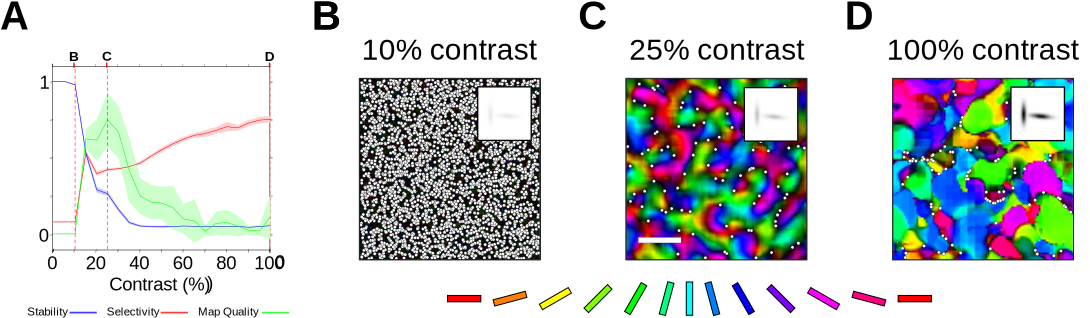
\includegraphics[width=1\textwidth]{./figures/L.pdf}
}
\caption[]{{\bf Analysis of the L model robustness in terms of
    selectivity, stability, and the new map quality metric.} (A) Mean map
  stability (green), selectivity (red), and map quality (blue) as a
  function of contrast, across 10 simulations with randomized input
  sequences where the shaded areas indicate the 95\% confidence interval
  for each metric. The L model has a peak in the map quality for a
  narrow range of training contrasts. Lines marked B, C, and D indicate
  the contrast levels used to train the example maps shown in this
  figure. (B) Example orientation map trained at 10\% contrast, where no
  development occurs in this case. Inset shows example training pattern and white
  points indicate false-positive pinwheel locations resulting in a high
  pinwheel density and correspondingly low value for the map quality
  metric. (C) Example orientation map trained at 25\% contrast, where the
  map quality metric peaks. White bar shows the hypercolumn distance, when it is possible to 
  estimate from the Fourier power spectrum. At this contrast, many
  pinwheels are correctly identified. (D) At 100\% contrast, the map is
  distorted, resulting in clusters of false pinwheels and a
  correspondingly low map-quality metric.}
\label{fig:L_model_metrics}
\end{figure}

Having an automated metric that can be used to summarize the quality of
many maps at once, allows this sort of observation to be made
easily. Without a metric, not only would it be difficult to justify any
particular subjective judgment but all $200$ orientation map simulations
that are succinctly summarized by the green trace would have to be
inspected manually.

Figure \ref{fig:L_model_metrics}B shows an example orientation map
illustrating how the L model behaves at low contrast. In this regime,
map organization did not take place, as there was no activity in V1 to
drive Hebbian learning and self-organization. In other words, the
afferent input to each V1 unit was insufficient to exceed the fixed
activity threshold. As a consequence, all units retained the initial
random orientation preferences assigned by the initial random weight
generation, resulting in a correspondingly low orientation
selectivity. As the preference structure does not change over
development, the stability metric is high. The lack of smooth
organization due to a lack of self-organization is responsible for the
low value for the map quality metric as a large number of false pinwheels
being detected, indicated by the white dots.

At high contrast, V1 suffers the inverse problem, with rapid changes to
the weights due to high pre- and postsynaptic activity, resulting in a
rapidly changing orientation map and consequently, low stability. There
is high orientation selectivity, but only because the last Gaussian training stimulus
is imprinted in the network weights. These distortions greatly increase the
pinwheel density, with many pinwheels found at the noisy boundaries where
the orientation preference values change abruptly.

\subsection{The AL model}

The AL model augments L with an adaptive, homeostatic threshold which
restores self-organization at low contrasts. If the initial threshold is
too high for a V1 unit to respond, the lack of activity will gradually
drop the threshold till the response is restored, allowing map
development to proceed.

With adaptation included, the map quality metric is close to one for low
contrasts but begins to drop as the contrast increases, as seen in
Figure \ref{fig:L_model_metrics}A. This is similar to the problem with
the L model when high contrast training stimuli are used. Although the
threshold of the V1 units rises due to the strong input, keeping the
postsynaptic activity within a suitable range, the presynaptic activity
is unaffected by this mechanism, resulting is rapid Hebbian learning
that distorts the map. The poor map organization results in clusters of
false pinwheels as well as unreliable hypercolumn distance estimates as
the size of hypercolumns begins to vary wildly. This unreliability in
the hypercolumn distance is a major contribution to the variance in the
map quality metric at high contrast.

\begin{figure}
\centerline{
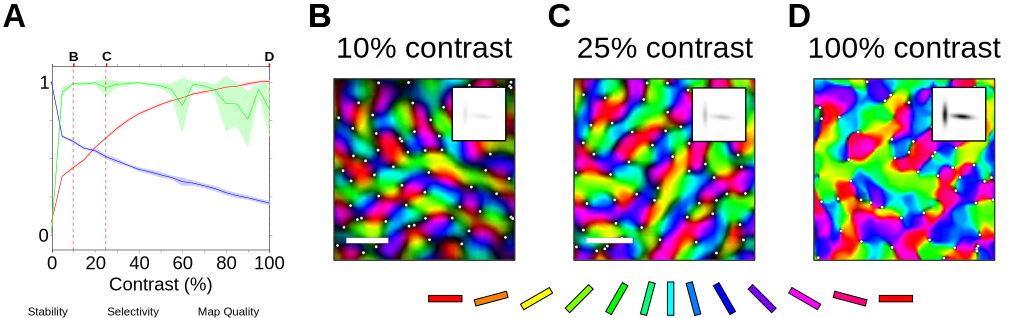
\includegraphics[width=1\textwidth]{./figures/AL.pdf}
}
\caption[]{{\bf Analysis of the AL model robustness in terms of
    selectivity, stability, and the new map quality metric.}
  [Same conventions as in Figure \ref{fig:L_model_metrics}.]
  The AL model has develops high-quality maps for low-contrast inputs
  (B and C, with high map metric, well-identified pinwheels, and
  accurately estimated hypercolumn distance).  However, at higher
  contrasts (e.g. C), it gives highly variable performance and
  low-quality maps, with clusters of false pinwheels that resemble the
  L model.}
\label{fig:AL_model_metrics}
\end{figure}

Without the map quality metric, it would be difficult to judge whether
the AL model performs well at high contrast from the mean stability and
selectivity curves, given that stability decreases but selectivity
increases. The example map in Figure \ref{fig:L_model_metrics}D does
illustrate the sort of distortions that are occurring but it is the map
metric that helps conclusively show that these distortions are occurring
across all the high contrast simulations.

\subsection{The GCL model}

The GCL model removes the homeostatic adaptation mechanism and
implements contrast-gain control in the ON/OFF sheets instead. This
results in the regulation of the presynaptic activity which also boosts
map quality at low contrasts, with the gain control mechanism boosting
weak stimuli to the point where V1 units receive sufficient input to
respond even with a fixed threshold.

The GCL model is more robust than the AL model at high contrasts, with
contrast-gain control regulating the presynaptic response of the
afferent projections. For the training patterns strong enough to drive
development, as shown in Figure \ref{fig:GCL_model_metrics}C and D, the
pinwheel density of the GCL model is close to $\pi$ with some small
additional variance.

\begin{figure}
\centerline{
\includegraphics[width=1\textwidth]{./figures/GCL.pdf}
}
\caption[]{{\bf Analysis of the GCL model robustness in terms of
    selectivity, stability, and the new map quality metric.} (A,B,C)
  [Same conventions as in Figure \ref{fig:L_model_metrics}.]
  For relatively high-contrast inputs, the GCL model has a
  consistently high map quality with relatively low variance. The
  metric fails to reach 1.0 because some small areas of the map never
  self-organize, consistently being inhibited by their
  sooner-developing neighbors and thus unable to learn the input
  patterns.}
\label{fig:GCL_model_metrics}
\end{figure}

The map quality of the GCL model is consistently high, but there are some
noisy regions that remain, in low selectivity areas of the map. These
artifacts correspond to areas of the map that have failed to develop
properly due to strong lateral inhibition by other highly responding
units in the vicinity. These noisy regions are not smooth, resulting in
small clusters of false pinwheels that lower the map quality and result
in the variance of the green curve in Figure \ref{fig:GCL_model_metrics}A.


\subsection{The GCAL model}

GCAL is the final developmental model that will be analyzed with the map
quality metric and this model is the one that will be extended in the
next chapter. GCAL simply combines the cortical adaptive threshold
mechanism of the AL model with the subcortical contrast-gain control
mechanism of the GCL model.

As Figure \ref{fig:GCAL_model_metrics} shows, GCAL is an incredibly
robust model that is both stable and selective, and also very reliably
develops maps with close to
$\pi$ pinwheel density. As soon as GCAL is driven strongly enough for
development to occur, the final map selectivity and developmental
stability is consistently high across contrast. Furthermore, the map
quality metric is nearly indistinguishable from unity, with very little
variance.

\begin{figure}
\centerline{
\includegraphics[width=1\textwidth]{./figures/GCAL.pdf}
}
\caption[]{{\bf Analysis of the GCAL model robustness in terms of
    selectivity, stability, and the new map quality metric.}
  [Same conventions as in Figure \ref{fig:L_model_metrics}.]
  The GCAL model has high selectivity, high stability
  and a nearly perfect map quality metric value ($\pi$ pinwheel
  density) for all contrasts where any self-organization occurs.}
\label{fig:GCAL_model_metrics}
\end{figure}


As GCAL model was developed prior to and independently of the map
quality metric, the discovery that GCAL orientation maps are close to
$\pi$ pinwheel density is an important validation of both the model and
the metric. The map quality metric served its purpose well, by
quantitatively supporting earlier subjective judgments regarding map
quality in the L, AL, GCL, and GCAL models that led to the design of
GCAL.

\section{Discussion}

The map quality metric introduced in this chapter has now been applied
in the context of a real analysis that led to the publication of the
GCAL model \citep{stevens_jn13} attached in the Appendix. Although the
GCAL model existed prior to this work, in the absence of a map quality
metric, it was difficult to conclusively demonstrate that GCAL formed
high quality orientation maps. In other words, it was not possible to
perform the kind of quantitative analysis that has been presented here.

The map quality metric proved vital in analyzing the L, AL, GCL, and GCAL
models for four reasons: (1) it is an orthogonal measure to the
selectivity and stability measurements, which cannot be omitted in a
detailed analysis of how the mechanisms in the GCAL model affect the process
of development, (2) it is independently informative, revealing
information that would be otherwise be difficult to assess, such as the
contrast value at which the L model has the highest quality maps (a
reference point that was then used throughout the analysis), (3) it
offers a well-defined, unambiguous, species-independent reference value,
unlike the mean map selectivity, for instance, and (4) it quantitatively
validates the primary output of the GCAL model, allowing it to be
presented to the scientific community, without having to resort to
subjective quality assessments.

To further illustrate the point regarding the orthogonality of the map
quality metric, it is feasible for a model to have exactly the same
selectivity and stability profiles as presented in part A of Figures
\ref{fig:L_model_metrics}--\ref{fig:GCAL_model_metrics} without ever
having organized into something other than a salt-and-pepper
arrangement. If this had been the case, GCAL would have failed as a
model of smooth orientation map formation, demonstrating that a high
pinwheel metric value is not simply desirable, it is \emph{necessary}.

Although the concept of pinwheel density and $\pi$ pinwheel density is
not novel, this is the first time it has been used as a metric to assess
this type of self-organizing map model. Pinwheel density has now been used
in the evaluation of other map-forming models, typically by showing a
violation of the $\pi$ pinwheel-density criterion using analytical
approaches. For instance, the stochastic wiring model proposed by
\citet{ringach_natneuro11} has been demonstrated to be unable to satisfy
$\pi$ pinwheel density \citep{schottdorf_plos15}. In addition, the
elastic net model is also unsatisfactory, as $\pi$ pinwheel density can
only be achieved by freezing development at a particular point in time
\citep{keil_neuralsys11}.

Unlike these other classes of model, there is currently no way to reason
about the eventual properties of orientation maps during development
when working with self-organizing map models, apart from running a numerical
simulation. As a consequence, the map quality metric has been used to
directly compare the properties of the observed model map at some stage
of development with the experimental constraint derived from maps in
mature animals.

The use of $\pi$ pinwheel density as an automated metric to assess these
particular models also had to be justified carefully. In section
\ref{section:map_metric_in_simulations}, it was necessary to reason
about the way in which the pinwheel location and hypercolumn distance
estimation algorithms fail for non-biologically plausible inputs. This
showed that poor quality maps tend to fall into the long tail of the
gamma squashing function where pinwheel density values are high. In
other words, poorly organized or undeveloped maps will have high
pinwheel density and it is the self-organization process that
brings the value closer to $\pi$.

This is partly because the developmental map simulations we are
considering have a randomized initial configuration and partly because
map distortions and other defects tend to appear noisy. A metric based
on $\pi$ pinwheel density may not be suitable when assessing other
classes of model. For instance, suppose a model where the orientation
maps are always guaranteed to be smooth and where striped configurations
are possible, such as the one shown in Figure
\ref{fig:synthetic_pi_density}A. In this case, there a possibility that
an implausible map might have close to $\pi$ pinwheel density purely by
chance. An underlying striped configuration could have a pinwheel
density below $\pi$ and some other effect might then act to bring the
pinwheel density closer to $\pi$ reference value.  Thus even though
the pinwheel-density metric has been very successful for these
models, it may not be appropriate for every type of model.

\section{Conclusion}

GCAL was a simple, stable, and robust model of orientation map
development prior to the start of this research project. The map quality
metric and analysis approach developed in this chapter was necessary to
validate the model by demonstrating these properties in an objective
way. Establishing a convincing way to analyze the plausibility of map
development in models such as GCAL was a key part of bringing this model
to publication.

The map metric based on pinwheel density allows map simulations to be
evaluated in terms of the spatial organization of orientation preference
in way that is independent of the species targeted by the model, so long
as it is a species with smooth maps. By showing GCAL has close to
$\pi$ pinwheel density, this metric demonstrates that GCAL has nearly
perfect orientation maps once border effects are reduced with respect
to this empirically determined criterion. Validating GCAL in this way in
order to get it published is also important for the work in the
following chapter that extends GCAL to construct a mechanistic and
spatiotemporally unified model.



\chapter{Unifying developmental and evoked response dynamics}
\label{chapter:TCAL}

The evoked response in the primary visual cortex is a reflection of the
ongoing state of the visual world in the context of long term visual
experience. For the activity of a neuron to represent meaningful
information, it must capture the state of a visual feature within a
space of possible outcomes, defined by the long-term statistical
properties of the environment in which the organism lives.

The response of an individual cortical neuron is only meaningful and
biologically relevant when considered in a broad context spanning time
and space, as discussed in Section
\ref{section:developmental_modeling}. The activity of a particular
neuron isolated from its surroundings is not the same as the visual response,
which only emerges from the dynamics of a large population. Similarly, a
network of neurons that has not captured the overall, long-term
statistics of the visual environment cannot perform any meaningful
computation, as the information content of a visual feature is only
defined with reference to the expected or learned properties of the
environment. 

This means that the dynamics of visual perception is determined by the
entire history of interaction between an extended volume of neural
tissue and the environment. As a result, any complete and mechanistic
model of vision must simulate a large population of neurons over a long
period of time. Unfortunately, even with state-of-the-art supercomputing
resources, it is not yet possible to run a detailed cortical spiking model
over the necessary spatial and temporal scales.  Moreover, the vast
number of parameters such a model would require would be greatly
underconstrained by the data, making the results unlikely to
correspond to meaningful aspects of the system being simulated.

Building a manageable model that spans the large spatial and temporal
scales relevant to the visual process must therefore use appropriate
simplifying approximations to reduce computational and parameter-space
complexity. One way
this can be achieved is to ignore the detailed biophysical properties of
individual neurons and use rate-based approaches to approximate the
spiking response of small collections of neurons at once. The SIRD and
GCAL model of Chapters \ref{chapter:SIRD} and \ref{chapter:GCAL} are
both rate-based models, but they cover very different timescales,
i.e.\ 200 milliseconds vs.\ days or weeks, respectively.  The goal of
this chapter is to build a single model that can bridge these levels
of description. 

The approach used to construct this model is to gradually extend GCAL,
improving its temporal properties until it can begin to incorporate the
insights of the SIRD model. This progression of features is shown in
Table \ref{table:Model_features}, starting with a new continuous version
of GCAL (\mbox{CGCAL}) that shows how developmental map models can
operate using a more realistic model of temporal processing. Next, this
continuous GCAL model is calibrated against PSTH profiles in the LGN and
V1 to form the TCAL (Temporally CALibrated GCAL) model. This yields a
developmental model that has appropriate single-unit evoked responses
and that can incorporate the mechanisms suggested by the SIRD model.

The final result is a new type of model that can simulate cortical
development as well as the detailed temporal dynamics of the evoked
response, within a single conceptual framework. Using this approach, it
is possible to explore how gradual activity-dependent learning processes
shape the network structure, which in turn determines the cortical
response dynamics. This new modeling platform will allow neocortical
operation to be explored in a much more unified and holistic
manner.

\section{Discontinuous temporal processing in GCAL}

Self-organizing map models such as GCAL account for feature map
formation via activity-dependent synaptic plasticity mechanisms. The
shortest natural unit of time in these models when considering
naturalistic behavior of an animal is the visual fixation. Only within a
single fixation is it reasonable to assume that the image on the retina
will remain in a constant position, assuming that the visual scene is
also static.

In GCAL and related models, multiple simulation steps are computed per
fixation in order to settle the activity bubbles in the cortical
sheet that drive smooth map development. The key assumption made by this
class of model is that activity bubbles form within each fixation
before learning, so that the learning step and weight update can be
applied at one instant, just before the next training pattern is presented.

In an awake, behaving monkey viewing a natural scene, a fixation lasts
between 100 to 400 milliseconds in duration
\citep{gallant_neuroreport98}. As the GCAL learning rule is applied once per
training pattern, these values specify the bounds on the shortest
meaningful time period in these types of map forming model. Although
there are simulation steps needed to settle the activity bubbles, it is
only the final activity profile at the end of a fixation that has any
impact on the weights and therefore the eventual model state.

In short, this means that the activity in self-organizing map models
such as GCAL within a fixation are only calibrated with respect to the
final activity state at the end of each fixation. The evolution of
activity in the subcortical pathway as well as the cortical sheet from
the initial presentation of the training stimulus up to this point has
no direct effect on the developmental process. Expressed in real world units,
this means that the highest meaningful temporal resolution of GCAL
with respect to the developmental process is between 100 to 400 milliseconds.

\subsection{Discontinuities in the time domain}

There are three particular features of GCAL that are appropriate
optimizations for a developmental map model yet are inappropriate for a
temporal model of activity that has a high time resolution. All of these
features result in non-uniform handling of events with respect to time,
whereby particular steps in the simulation have a special significance
or are otherwise processed differently.

Any non-uniform processing in the model as a function of time points to
a potentially implausible mechanism, since the components of real biological
systems tend to have a smooth time evolution without dramatically
discontinuous behavior. A model without these discontinuities will now
be described as ``continuous'' even though the numerical simulation
involves discrete spatial sampling and discrete time steps. As will be
discussed shortly, this approach is a step towards building a truly
continuous model that would be expressed with differential equations
instead of difference equations.

Using this sense of ``continuous'', the Continuous GCAL model (CGCAL)
introduced in the next section eliminates the temporal discontinuities
in the GCAL model, namely the non-uniform timesteps, the elimination of
the initial LGN activity as projected to V1, and the periodic
scheduling of processes like the Hebbian learning step, the
adaptive threshold adjustment, and artificial activity reset.


\subsubsection*{Non-uniform time intervals between events}

The GCAL model is implemented as an event driven neural simulation
whereby events are scheduled to run after a specified delay. Each event
can trigger some processing which may in turn may trigger further
events. This is an efficient scheme for implementing developmental
models as different sheets are allowed to update at different rates, and
sheets where the activity is known to be held constant (such as the
photoreceptor sheet during fixation on a static scene) do not need to be
updated. For instance, in GCAL there are $16$ settling events in the V1
sheet for every $2$ events in the ON and OFF sheets which in turn are
triggered by a single event driven by the photoreceptor sheet as the
training pattern changes.

In a continuous model of response dynamics where the activities of all
the neural sheets are expected to always be varying with time, the
benefits of an event driven scheme are reduced and a clocked simulation
scheme becomes conceptually simpler. Using a clocked model, newly
computed activities are generated for all the units in every sheet of
the model at every timestep. It is then possible to assign a real world
time value to the timestep as we shall see shortly, making it easier to
compare the model responses with experimental recordings.

\subsubsection*{Snapshot learning, homeostatic threshold, and activity reset}

In order to be efficient, GCAL executes certain processes at a lower
rate than the maximal event rate associated with the recurrent lateral
settling in the V1 sheet. These processes must then be adjusted when
implementing a continuous model to approximate smooth temporal
evolution. Although there are events that appear discrete in the nervous
systems, such as action potentials or vesicle release, realistic processes
at the level of an individual GCAL model unit are likely to act
continuously, whether or not the time constant of the process is fast or
slow.

Snapshot learning refers to the way developmental self-organizing map
models wait for activity bubbles to emerge before the Hebbian learning
step is applied in order to form smooth feature maps. In addition to the
synaptic weight adjustment, the homeostatic threshold update is also
executed once the 16 lateral settling steps in the V1 sheet are
completed for any given training presentation.

This arbitrary waiting period of $16$ settling steps before update is
difficult to justify when attempting to model the response on a
millisecond timescale. There is an additional process that is also
clocked at a different rate, namely the activity reset that is triggered
when new afferent input is received. This reset to zero activity is
useful when trying to reason about developmental models as it ensures
that the dynamics within each fixation duration are independent of each
other for a given set of model weights.

When considering a continuous model, there is no reason to think that
activity in the cortex cannot persist from one moment to the next. In a
naturalistic free viewing condition, saccades that last 20-40
milliseconds do serve as a natural separation between fixation
\citep{gallant_neuroreport98} events. Although these intervals can help
justify activity resets, the correct approach in a continuous model is
to appropriately modify the cortical input and not to instantaneously
eliminate all activity between fixations. As we will see next, there
is another way activity is instantaneously suppressed in the GCAL
model.


\subsubsection*{Suppression of initial LGN activity to V1}

In GCAL there are two steps involved when processing activity in the ON
and the OFF RGC/LGN sheets. First the initial activity is projected from
the photoreceptor sheet to the LGN sheets via the
difference-of-Gaussians center-surround weights. This initial activity
is \emph{not} 
projected onwards to the V1 sheet but is then used to compute a new
activity in the RGC/LGN sheet in a single step, via the action of the
lateral divisive projections used to implement contrast-gain
control. Only after the application of this contrast-gain control is the
activity projected to the cortical sheet.

In other words, the dynamics of subcortical contrast-gain control are
implemented as a one step process in the ON/OFF sheets and entirely
invisible to the cortical sheet. In this way, whatever transient
response of the gain control mechanism may have is ignored.  Although
this simplification is appropriate for the purposes of developmental
modeling, it is not appropriate in a model explicitly designed to
explore the properties of transient responses.


\subsection{Converting GCAL into a continuous model}
\label{section:CGCAL}

The Continuous GCAL model (CGCAL) is designed to be as similar to GCAL
as possible while removing the issues with discontinuous temporal
processing mentioned above. All spatial parameters of the GCAL are left
unchanged and the settings of CGCAL are chosen to mimic those of the
original model as closely as possible. Unlike GCAL, CGCAL is a clocked
model without activity resets, featuring continuous learning, continuous
homeostatic adaptation and continuous contrast-gain control in the
ON/OFF sheets.

Each of the following subsections detail the corresponding fix to each
of the issues listed in the previous section. Some of the
necessary changes were first introduced in \citet{stevens_ms11} in an
early non-developmental version of TCAL that did not include a continuous
version of GCAL, but the formulation developed in this thesis helps
separate the effect of each mechanism. CGCAL and TCAL are also now complete
developmental models that support scalable timesteps by automatically
recalculating the various learning rates, allowing simulations to be
run using different temporal resolutions.


\subsubsection*{Clocked simulation}

In order to be able to sample unit responses across all stages of the
model on a consistent timebase, it is necessary to use a clocked
simulation. The original event driven model can be adapted by emitting
new events every $0.05$ time units from the photoreceptor sheet to drive
the activity in the rest of the model. Then it is necessary to ensure
that all the projection delays in the model are integer multiples of
this timestep to make sure that all the sheets will be updated in
lock step, without any updates occurring at fractional timesteps.

This conversion to a clocked mode does not have a major impact on the
behavior of GCAL, as all projection delays were already multiples
of the minimum $0.05$ value used to settle activity in the cortical
sheet. After clocking the photoreceptor sheet, all stages of the CGCAL
model are updated $20$ times per training pattern presentation,
corresponding to one unit of simulation time which also corresponds to a
single fixation. This modification ensures that the LGN sheet will also
receive $20$ multiple events from the photoreceptor layer per simulation
time. This will then reveal the activity dynamics of the contrast-gain
control mechanism in the ON/OFF sheet that were previously implemented
as a single step process.


\subsubsection*{Continuous sheet model}

The original GCAL model makes use of a customized implementation that
enforces an exact number of settling steps in the cortical sheet before
waiting for a new input event. This parameter offers extra control that
is helpful when optimizing a developmental, event driven simulation, but
is unsuitable for a continuously clocked model. There is no
reason to expect lateral interactions to stop occurring after a fixed
number of steps, when the activity state is not being reset between
fixations. This activity reset and the periodic learning are implemented
in this sheet and we have seen that these mechanisms pose a problem for
a continuous model.

To address this, a simpler, continuous sheet type was implemented for
use by the CGCAL model that processes all incoming events in a uniform
way. This new implementation removes the activity reset and ensures that
the Hebbian learning rule is applied every timestep. Using this sheet in
the LGN means that the initial transient response of the ON/OFF sheets
is no longer suppressed from reaching V1.

Together the clocked photoreceptor layer, the continuous sheet
implementation addresses most of the issues described in the previous
section. In the ON and OFF sheets where Hebbian learning is disabled, it
results in a more consistent and continuous application of contrast-gain
control while in V1 sheet, it enables continuous learning without
activity resets or an enforcing number of settling steps.

\subsubsection*{Rescaled learning rates}

Using a continuous sheet requires some of the parameters of the GCAL
model to be rescaled, as each mechanism will now be invoked more
frequently than before. In particular, parameters relating to time
constants or learning rates need to be adjusted, as these implicitly
depend on the timestep in GCAL.

By default, the V1 sheet of the CGCAL model applies Hebbian learning
once every $0.05$ timestep, instead of once per fixation as in GCAL. As
a result, the learning rates associated with the afferent and lateral
projections in V1 must be adjusted to compensate. Now that the model is
clocked in increments of $0.05$, there are $20$ simulation steps per
simulation time unit. Dividing the Hebbian learning rates by this number
then helps keep them in line with the original model.

The homeostatic threshold adaptation mechanism in V1 also needs to be
adjusted as it is also being invoked $20$ times more frequently per unit
of simulation time. In other words, the per-unit homeostatic thresholds
in the CGCAL model are updated over the course of the response within a
fixation, and not just at the end of it. Like the Hebbian learning
rates, the homeostatic learning rate is simply divided by $20$, that is
to say the number of timesteps per unit of simulation time (i.e. per
fixation).


\subsection{Behavior of the CGCAL Model}

The aim of the CGCAL model is to reproduce the behavior of GCAL without
the discontinuous temporal properties of some of its mechanisms. As this
required some significant changes to the sheet implementation as well as
learning rates, it is necessary to examine the behavior of the CGCAL
model relative to GCAL. First the subcortical pathway will be considered,
in order to ensure that the temporal response profiles in the ON/OFF
sheets are still consistent with the original model.

Figure \ref{fig:CGCAL_LGN} compares the temporal responses of the ON
sheet, sampled using a regular spatial grid. These temporal response
profiles are obtained from the projection activity, i.e., the
activity from the ON sheet as it is projected to V1. This is the reason
there is no sharp initial peak in activity in the GCAL profiles, resulting
in simple step profiles.

In the middle of the figure, the responses are shown for the new
Continuous-GCAL model as it has been described so far. The initial
transitory activity peak is now clearly visible, driven by the initial
activity from the photoreceptor sheet, through the LGN, showing the
early response before contrast-gain control in the ON/OFF sheets can be
applied. The subsequent oscillatory response reveals that the
contrast-gain control mechanism has its own dynamics that was entirely
obscured when gain control was implemented as a one step process. Now that there
are just as many events occurring in the ON/OFF sheets as the cortical
sheet, it is clear that settling dynamics is a feature of all the
visually driven sheets as the response approaches a steady state.


\subsubsection*{LGN Hysteresis}

The oscillatory temporal profiles of activity in the ON/OFF sheets of
CGCAL are now different from the step profiles received by the V1 units
of GCAL. This motivates the introduction of the one new mechanism that
is present in the CGCAL and subsequent TCAL models but is not already
present in GCAL.

Activity hysteresis can be applied to the continuous ON/OFF sheets of
CGCAL to dampen the oscillatory behavior and make the profiles more
similar to those in GCAL. This mechanism smooths the activity over time
using an exponential falloff, defined by the hysteresis time constant
$\tau$.

The following equation expresses hysteresis in terms of the unit
activities $\eta$ between one simulation timestep and the next. The
activity value after hysteresis, ($\bar{\eta}_t$) is computed using the
time constant $\tau$, the current input activity ($\eta_t$) and the
previous input activity ($\eta_{t-1}$) where these input values
correspond to the half-rectified activity output of the unit, before the
action of hysteresis:
%%
\begin{equation}
  \bar{\eta}_t = \bar{\eta}_{t-1} + \tau (\eta_t - \eta_{t-1})
  \label{eq:hysteresis}
\end{equation}
%%
Using a dimensionless time constant of $\tau_{LGN}=0.6$ in the new
hysteresis mechanism after half-rectification, it is possible to make
the ON and OFF responses much more similar to those of the original
model. This can be seen in Figure \ref{fig:CGCAL_LGN} by comparing the
grid of ON sheet PSTH profiles on the left (GCAL) and right (CGCAL with
the hysteresis mechanism). At this point it is worth noting that these
are \emph{not} plausible PSTH profiles for LGN cells, illustrating the
point that GCAL was only calibrated with respect to the cortical
activity at the end of the fixation period. Calibration of these
profiles will be done in section \ref{section:TCAL_PSTH_calibration}.


\begin{figure}
\centerline{ 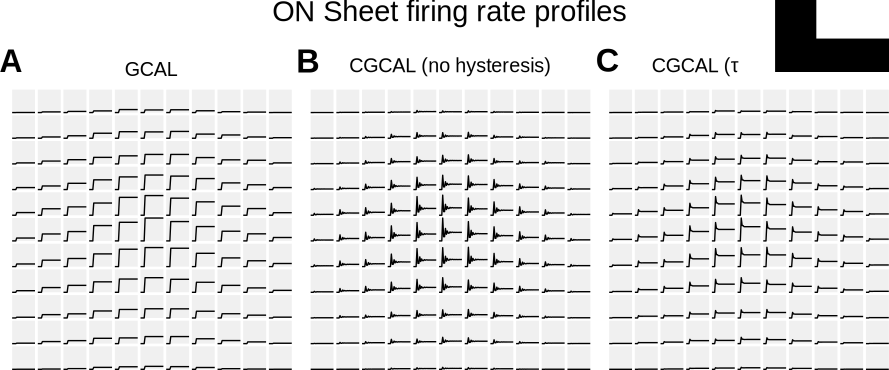
\includegraphics[scale=0.6]{./figures/CGCAL_LGN.pdf} }
\caption[]{{\bf Comparison of ON sheet responses as received by V1 units
    in the GCAL and CGCAL (with and without hysteresis) in response to
    an isotropic Gaussian stimulus.} (A) The GCAL profiles are simple
  step functions as the initial activity before contrast-gain control is
  not propagated to V1. (B) CGCAL response as a direct analog of GCAL
  without any additional mechanisms. Responses do not match the profiles
  on the left due to recurrent action of lateral inhibition within the
  RGC/LGN sheets. (C) adding a small amount of activity hysteresis
  brings the CGCAL model closer in line with the GCAL response. Similar
  results can be obtained by analyzing the OFF sheet responses with
  profile amplitudes which have an inverse relationship across space.}
\label{fig:CGCAL_LGN}
\end{figure}


Equation \ref{eq:hysteresis} is a difference equation and it is defined
in terms of a dimensionless constant, $\tau$. Choosing any specific
$\tau$ value means that the response dynamics will depend on the
timestep size, which in this case is $0.05$ simulation time units. In
order to avoid a strong dependence on the timestep value, it is
appropriate to define the hysteresis time constant in \si{ms^{-1}}. The
hysteresis constant used in the CGCAL ON/OFF sheets is then $0.05
\si{ms^{-1}}$, as shown in Figure \ref{fig:CGCAL_LGN}C.

Computing the dimensionless $\tau$ value required by Equation
\ref{eq:hysteresis} from the $\tau$ value specified in terms of
milliseconds is straightforward: simply multiply by the timestep
duration in milliseconds. So far, no real world duration has been
assigned to a timestep in GCAL, but this is also easy to compute from
the values already stated.

If one simulation time unit corresponds to a single fixation which we
will assume to last $240$ milliseconds, the $20$ simulation steps in
this period means that each timestep is separated by $12$
milliseconds. We can now compute the corresponding dimensionless
hysteresis value using in CGCAL by multiplying $\tau_{LGN}=0.05
\si{ms^{-1}}$ by $12$ milliseconds to get $\tau_{LGN}=0.6$.

This hysteresis constant scaling equation together with the scaling
equations for Hebbian and homeostatic threshold learning allows the
timestep size to be adjusted, within limits. If the timestep is too
large, there will be insufficient simulation steps for these equations
to act appropriately.  The values may also need adjustment in the
continuous limit, as the timestep approaches zero.

As all the dynamical equations of the CGCAL model are now expressed in
terms of difference equations that update the model between time $t$ and
time $t+1$ without adding discontinuous behavior, it should be straightforward
to reformulate the model in terms of differential equations in
future. Expressing CGCAL using differential equations might enable the
use of analytical techniques that could not be applied before. Such an
analysis could prove useful, even if the numerical simulations
continue to rely on an approximation based on difference equations.

\subsubsection*{CGCAL response}

Now that the subcortical responses in the CGCAL model have been adjusted
to match those of GCAL, it is possible to explore the difference in
behavior between these two models. In particular, it is instructive to
visualize how activity bubbles form as the training pattern presented
to the photoreceptor sheet changes in spatial position.

Figure \ref{fig:V1_activity_CGCAL} illustrates one of the main
differences between CGCAL and previous developmental map models such as
GCAL. As a training pattern is presented, activity bubbles form, as is
required for smooth orientation map formation in a self-organizing map
model. In CGCAL, unlike GCAL, the Hebbian learning rule is now being
applied on every timestep, as is the homeostatic threshold update.

The difference in activity dynamics between the two models is
highlighted when the training pattern changes and new afferent input
arrives in the V1 sheet. In GCAL, all the activity in the V1 sheet is
reset, with bubble formation starting anew from a condition of zero cortical
activity. In CGCAL, there is no artificial temporal boundary between
training patterns, and so when the stimulus changes, the existing activity
bubbles may either decay, shift position, or get reinforced by additional
incoming activity.

\begin{figure}
\centerline{ 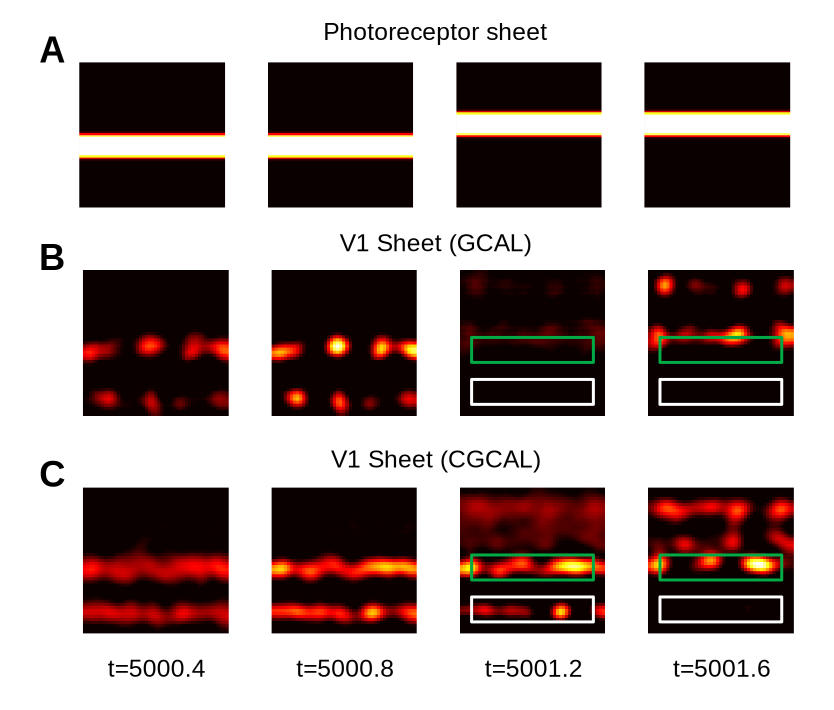
\includegraphics[scale=0.7]{./figures/V1_activity_CGCAL.pdf} }
\caption[]{{\bf Comparison of responses to horizontal line in GCAL and
    CGCAL models after $5000$ training iterations.} (A) The horizontal
  line pattern presented on the photoreceptor sheet at times $5000.4$,
  $5000.8$, $5001.2$, and $5001.6$ with the pattern appearing at iteration
  $5000$ with zero activity in the V1 sheet at that time. (B) The
  activity response in the GCAL model to the horizontal line at the
  indicated times. Between $t=5000.4$ and $t=5000.8$, the activity
  bubbles are seen to get stronger. As the horizontal line shifts
  between $t=5000.8$ and $t=5001.2$, the activity reset is triggered,
  eliminating all activity in the V1 sheet. Between $t=5001.2$ and
  $t=5001.6$ the activity bubbles build up in the top half of the
  cortical area. (C) Corresponding response in the CGCAL model. At the
  start, between $t=5000.4$ and $t=5000.8$ activity bubbles start
  forming as before. The activity is not reset by the change in line
  position leaving residual activity in the white rectangle at
  $t=5001.2$ which later decays away. In some areas, the residual
  activity persists from the previous stimulus position only to be is
  reinforced by the new stimulus (green rectangle).}
\label{fig:V1_activity_CGCAL}
\end{figure}

The stimulus used in Figure \ref{fig:V1_activity_CGCAL} corresponds to a
fixation switching between two static scenes, in order to allow direct
comparison with GCAL. It is worth noting that CGCAL supports more
interesting behavior than GCAL, as you could present a moving stimulus
within each fixation in order to simulate motion. Motion and direction
maps have been simulated in self-organizing map models before
\citep{bednar_jpp12,miikkulainen_2005} but temporal processing in
these models was discontinuous, and here a more appropriate model of
time could be used in future simulations.  Using
spatiotemporal stimuli for analysis and training is discussed in
section \ref{section:future_image_statistics}.


\subsubsection*{CGCAL OR map development}

Having defined CGCAL and having investigated the response of the ON/OFF
and cortical sheets to a single stimulus, it is time to verify that
CGCAL still works as a developmental map model. Figure
\ref{fig:CGCAL_OR_map} shows an example of a GCAL orientation map next
to an example of a CGCAL orientation map. Although CGCAL does not have
an orientation map as high quality as the GCAL reference, it is clear
that smooth map formation is retained in the CGCAL model, despite the
numerous changes to the dynamics.
%%
\begin{figure}
\centerline{ 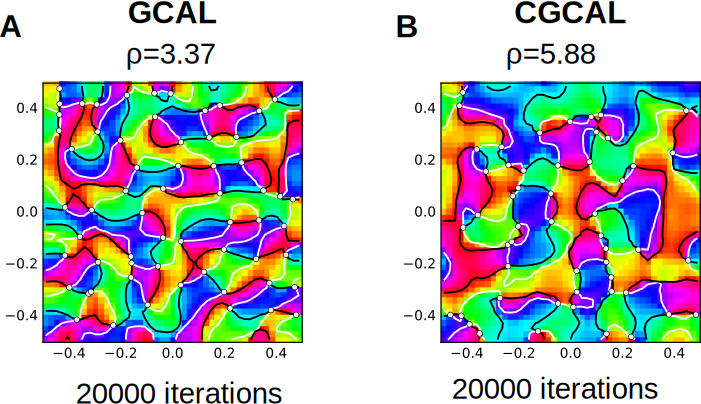
\includegraphics[scale=0.5]{./figures/CGCAL_OR_map.pdf} }
\caption[]{{\bf Comparison between GCAL and CGCAL orientation maps after
    $20000$ iterations.} On the left is an example GCAL orientation map
  after $20000$ iterations and on the right is the corresponding CGCAL
  map. Both maps are annotated with pinwheels as well as the real
  (white) and imaginary (black) contours in the polar representation.
  Both maps were generated using the same stream of randomized training
  patterns.}
\label{fig:CGCAL_OR_map}
\end{figure}
%%
At this point, the CGCAL model is complete, having demonstrated the
minimal set of changes necessary to redefine GCAL as a continuous,
clocked simulation with smooth map formation.

The CGCAL orientation map in Figure \ref{fig:CGCAL_OR_map} is clearly
less realistic than the GCAL map, which is likely because the activity
bubbles are not as clear as they are in GCAL (see Figure
\ref{fig:V1_activity_CGCAL}).  With parameter tuning to achieve more
well-formed bubbles, there is no reason to assume that $\pi$ pinwheel
density could not be achieved in CGCAL, as all the relevant mechanisms
are inherited directly from GCAL. However, this tuning falls outside
the scope of CGCAL, which is explicitly designed to retain all of
GCAL's parameters when possible so that we can use it to establish a
link between GCAL and the TCAL model to be introduced later in this
chapter.

At this juncture, two possible descendents of the CGCAL model can be
considered. One would explicitly re-tune the parameters to achieve the
same, high-quality orientation maps as GCAL, but now in the continuous
framework. The second route is to improve the shape of the response
profiles in the ON/OFF and V1 sheets. The dynamics of the response in
the RGC/LGN sheets are particularly interesting, as CGCAL has revealed
dynamics that were previously suppressed. Improving the plausibility of
these responses is the goal of the TCAL model, described in the next
section.

\section{TCAL: Temporally CALibrated}
\label{section:TCAL}

The argument so far is that CGCAL has a more plausible model of temporal
processing than GCAL. As the map quality has decreased and a new
hysteresis mechanism had to be introduced to match GCAL, this model does
not appear to be an improvement in terms of any concrete results. In
addition, by throwing away the optimizations used in GCAL, each
simulation run is much slower, with $20\times$ more learning and
homeostatic update steps for no obvious benefit in explanatory power.
Here we will treat CGCAL as just a step along the way to a more
powerful model, TCAL.

TCAL is a direct descendent of CGCAL that, for the most part,
only requires some parameter re-tuning to demonstrate something
completely new. It is still a developmental model, but unlike previous
developmental models, the dynamics of the activity response within each
fixation period are calibrated. Temporally CALibrated GCAL model (TCAL)
has exactly the same structure as CGCAL but it makes contact with the
experimental data regarding the evoked activity response, as well as with
the SIRD model of Chapter \ref{chapter:SIRD}.

To start with, the timebase will be remapped so that one simulation time
unit is intended to correspond directly to a one millisecond
duration. Applying this simple, linear transformation will make it
easier to compare TCAL responses with the experimental data.


\subsection{Temporal resolution and simulation duration}

By convention, one simulation time unit corresponds directly to one
millisecond in TCAL. By default, each training pattern is presented to
the photoreceptor sheet for the duration of one fixation, lasting $240$
milliseconds. This value falls near the middle of the $100$ to $400$
millisecond range of fixation durations observed in monkeys viewing
natural images \citep{gallant_neuroreport98}. The default timestep
between simulation updates is $5$ milliseconds, chosen to offer a good
compromise between overall execution time and temporal resolution. As
TCAL inherits the timestep scaling equations from CGCAL, it is always
possible to adjust the timestep if required.

With $5$ millisecond timesteps within each $240$ fixation, there are now
$48$ simulation steps per training pattern in TCAL instead of the $20$
steps executed in CGCAL. In line with GCAL, the goal in TCAL is to form
orientation maps within $10000-20000$ training iterations.

Assuming this constraint is satisfied, it is now possible to compare the
time taken for orientation developmental in a real animal to the
corresponding simulation time expressed in milliseconds. It is expected
that development in the model will happen quickly as using an elevated
learning rate is one way to reduce the computational cost of running a
developmental simulation. Using TCAL, it is possible to get an idea of
how much faster learning occurs in the model than it does in real time.

A simulation of $20000$ fixations of $240$ milliseconds each corresponds
to around $1.3$ hours of real visual input, ignoring the duration
between fixations. For comparison, orientation map development in ferret
as recorded with chronic intrinsic optical imaging takes several days as
shown in Figure \ref{fig:ferret_stability}. Although an $11$ day time
period is shown, the initial map structure forms in around two days,
between p31 and p33. In addition, the electrophysiological measurements
of selectivity shown in Figure \ref{fig:chapman_data} suggest that map
development may be essentially complete by p39.

Even if you consider the lack of visual input from the external world
during the periods of sleep, it is clear that the learning rate used in
developmental models is very high when compared to the experimentally
observed development process. Matching the rate of change induced per
fixation would require a learning rate that is a hundreds times slower,
or alternatively, simulations that take hundreds of times longer to run.

Achieving such a match is not useful here, as the purpose of a developmental
model is to capture the processes involved in forming receptive fields
and understanding how they are organized across the cortical surface. If
TCAL can demonstrate that units are learning suitable weight
patterns and that a self-organizing process is taking place, then it
will be successfully modeling a phenomenon that emerges on a timescale of
days. The stated time in milliseconds at the end of a simulation run
then has to be interpreted cautiously, due to the elevated learning
rate.

This example illustrates what is means for a model to span both the
timescales of development and the timescales of the evoked response. A
$5$-millisecond bin is a reasonable interval for collecting action potentials
and computing firing rate profiles to be calibrated against experimental
PSTHs. If the same model also simulates the emergence of orientation
maps, then means that the model is accounting for a developmental
process that takes place over several days. Over this timespan, the
tuning properties of the units emerge and there are large scale
structural changes to the cortex that affect its functional properties.

It is important to emphasize that TCAL can efficiently bridge these
timescales using modest computing resources. Compared to an equivalent
spiking level simulation of the same cortical area and over the same
timescale, TCAL is highly tractable. A TCAL simulation to $20000$ steps
will complete within around 6 hours using a modern server processor,
for the default area and density. It would be entirely feasible to
expand on the computational resources to achieve a model that operates
in real time with a more realistic learning rate such that a few days
running a simulation would correspond to a similar number of days of
cortical development.

\subsection{Calibrated single-unit response profiles}
\label{section:TCAL_PSTH_calibration}
TCAL will calibrated in two stages, first by considering the evoked
response timescale of milliseconds and then, by calibrating it on the
developmental timescale of days. The key question is whether the firing
rate responses of TCAL units can be made sufficiently plausible. In
other words, whether TCAL units can have realistic PSTH profiles in
relation to the experimental data.

Remarkably, it turns out that highly realistic temporal profiles
can be achieved without introducing any new mechanisms
at all. The only additional mechanism required by TCAL has already been
introduced in CGCAL, namely the hysteresis mechanism applied to the
ON/OFF sheets. This is where the first PSTH calibration will occur, and
we will see that the dynamics of contrast-gain control revealed by
CGCAL are sufficient to generate plausible PSTH profiles.

\subsubsection*{PSTH profiles in the LGN sheets}

How can a developmental model achieve plausible LGN PSTH profiles such
as the ones shown in Figure \ref{fig:LGN_PSTH_maunsell} without
requiring new mechanisms? A hint can be seen in Figure
\ref{fig:CGCAL_LGN}C, where we see the transient dynamics that were first
revealed by CGCAL and then suppressed again to try to match GCAL. In
TCAL, these transient dynamics are explored and tuned to generate
plausible PSTH profiles in the ON and OFF sheets.

In all the models we have considered, the initial activity in the ON and
OFF sheets is instantaneously high due to the high afferent drive from
the photoreceptor sheet. Then once the lateral inhibitory projection
implementing contrast-gain control becomes active, the ON and OFF activity is
reduced. In CGCAL, the additional simulation steps revealed oscillations
in the response as activity settled towards a steady state. These
dynamics were then suppressed in CGCAL to match GCAL, but in TCAL, it is
these exact network dynamics \emph{together} with hysteresis that
generate plausible firing-rate profiles.

What TCAL shows is that if the transitory oscillations have the right
frequency, they can then be appropriately damped to generate a plausible
PSTH profile. There are three parameters of CGCAL that can be tuned to
achieve this, without modifying the difference-of- Gaussian weights, the
afferent weight profiles, or the size of the lateral inhibitory
fields. These three parameters are (1) the lateral inhibitory delay of
the contrast-gain control connections, (2) the strength of the
contrast-gain control connections, and (3) the hysteresis time constant. Note
that the spatial sizes of these lateral projections do not need to be
modified from the values set in GCAL.

The necessary changes can be justified fairly directly. First, the
oscillations in Figure \ref{fig:CGCAL_LGN}C are very rapid and can be
slowed down by increasing the delay of the lateral inhibitory
contrast-gain control projection to $35$ milliseconds, up from $5$
milliseconds in CGCAL. Next, as we want to reveal the dynamics of this
settling, the lateral inhibitory strength is boosted from $0.6$ to
$8.0$. The result of these modifications are shown in Figure
\ref{fig:TCAL_LGN_PSTH}A using the same analysis procedure introduced in
Figure \ref{fig:CGCAL_LGN}.

What these profiles show are the TCAL ON responses without hysteresis,
which now look very different from the step profiles of Figure
\ref{fig:CGCAL_LGN}A and C. These oscillations do not yet look like PSTH
profiles, as their gradient changes discontinuously during the settling
process, but the shape can be changed by introducing an appropriate level of
hysteresis.

In CGCAL, the hysteresis constant was set to $0.05$ \si{ms^{-1}} to try
to replicate the step shaped profiles of GCAL. In TCAL, this hysteresis
constant is slightly reduced to $0.03$ \si{ms^{-1}}, resulting in the
profiles shown in Figure \ref{fig:TCAL_LGN_PSTH}B. These profiles now do
appear to be similar in shape to smooth PSTH profiles.

The central PSTH profile of Figure \ref{fig:TCAL_LGN_PSTH}B is shown in
more detail in part C where it is compared to the average magnocellular
LGN PSTH in macaque \citep{maunsell_visneuro99}. Although the fit is not
perfect, it is certainly plausible and it is far more realistic than the
responses of previous developmental models, such as those shown in
Figure \ref{fig:CGCAL_LGN}.

\begin{figure}
\center
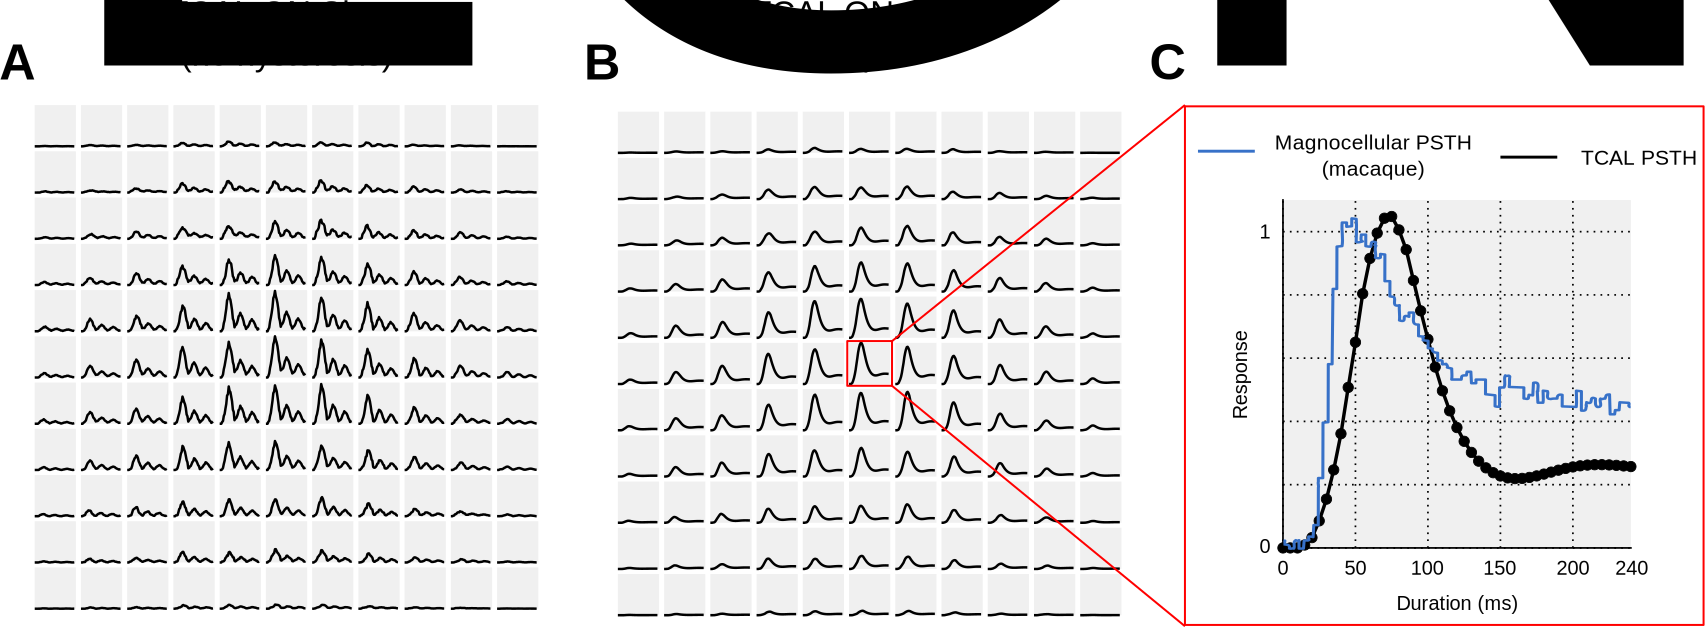
\includegraphics[width=1\textwidth]{./figures/TCAL_LGN_PSTH.pdf}
\caption{{\bf Activity profiles of TCAL ON sheet units, with and without
    hysteresis in response to a Gaussian spatial pattern presented on
    the photoreceptor sheet.} (A) Oscillatory behavior after tuning
  lateral inhibitory parameters in the ON and OFF sheets. (B) Smooth
  activity profiles after the application of hysteresis. (C) Comparison
  of activity profile of central unit marked in (B) with average of
  experimentally recorded PSTHs in macaque.  Blue trace shows average
  PSTH profile of 80 parvocellular LGN cells. Black trace shows TCAL
  activity profile with circles marking simulated sampling rate every
  $5$ milliseconds. Experimental PSTH reproduced from
  \citet{maunsell_visneuro99}.}
\label{fig:TCAL_LGN_PSTH}
\end{figure}

\subsubsection*{Biological origins of the PSTH profile}

It is remarkable that PSTHs emerge from the simple application of
hysteresis using a mechanism originally introduced to achieve robust
orientation map development. There is plenty of evidence for
contrast-gain control and similar mechanisms (see
\citealt{carandini_nature12} for a review), but is this a reasonable
explanation for the temporal pattern of the firing rate response?

The temporal firing rate profile of a cell is a function of its
particular internal biophysics and the way the inputs from the
surrounding network arrive at the cell over time. It is clear that the
interaction with surrounding cells is going to be an important
component in determining the PSTH profile for a cell's response.

In TCAL (as for GCAL and CGCAL), these network interactions are
modeled as lateral inhibitory
settling in the ON and OFF sheets. Each of these sheets represents the
combined properties of retinal ganglion cells and lateral geniculate
nucleus cells with ON and OFF difference-of-Gaussian
receptive-fields. It would be possible to apply one contrast-gain--control
projection across both populations, but this would not affect TCAL's
ability to generate these PSTH profiles. 

What the $35$ millisecond delay might represent is some average time
constant for action of contrast-gain control across space. What is
essential for this explanation to work is that the cell's activity is
allowed to rise to reach its maximum firing rate, before the
contrast-gain control mechanism has time to settle and bring the
response back down to an appropriate, sustained level. The key idea is
that the lateral network effects only act to reduce the response of the cell
after it has reached a high firing rate due to the afferent drive.

What is clear is that lateral interactions between cells across space
must exist in the visual system if the firing rate at one retinotopic
position is to affect the firing rate at a different retinotopic
position. Where these interactions occur is not specified by the TCAL
model as the retinal ganglion cell population and the cells of the
lateral geniculate nucleus are collapsed together according to their
receptive field types in the ON/OFF sheets. The PSTH profiles are then
explained by how fast the network interactions that implement
contrast-gain control are able to act.

Whether or not this explanation is correct, two things are clear: (1)
lateral inhibitory settling with hysteresis is sufficient to generate
plausible PSTH profiles in TCAL, and (2) as long as the input firing-rate
profiles are realistic in shape, the behavior in the cortical layer is
independent of the underlying mechanisms that determine PSTH shapes in
the ON/OFF sheets.

TCAL is a cortical model that requires realistically shaped input
profiles, which could hypothetically be generated by a sufficiently
detailed phenomenological model. The means by which TCAL does generate
PSTH profiles in the ON/OFF sheets is both extremely simple and
sufficient for the purposes of cortical modeling, independently of
whether lateral inhibitory settling is the true cause of the PSTH
profile shapes.


\subsubsection*{PSTH profiles in the V1 sheet}

With the temporal response profiles in the ON and OFF sheets calibrated,
absolutely no changes are required within the cortical sheet to obtain
the V1 PSTHs shown in Figure \ref{fig:TCAL_V1_PSTH}. The only parameter
that is modified is the afferent projection strength from the ON/OFF
sheets to V1 which is boosted by a factor of five to compensate for the
increased subcortical contrast-gain--control strength that reduces the
afferent drive to V1.

This result suggests that a major component of the temporal, single-unit
activity profiles in V1 is simply inherited from the corresponding
response dynamics in the LGN. This property follows naturally in any
mechanistic models where the evoked response in V1 is driven by the
spiking afferent inputs from the lateral geniculate nucleus.

In all the developmental models we have considered, the properties of
the ON/OFF sheets are fixed, with no subcortical plasticity. This
means that the profiles shown in Figure \ref{fig:TCAL_LGN_PSTH} remain
identical at all stages of development. In contrast, the cortical sheet
is plastic, which means the profiles shown in Figure
\ref{fig:TCAL_V1_PSTH} will change over time as Hebbian learning updates
the network structure and as the adaptive homeostatic thresholds vary
over time.


\begin{figure}
\center
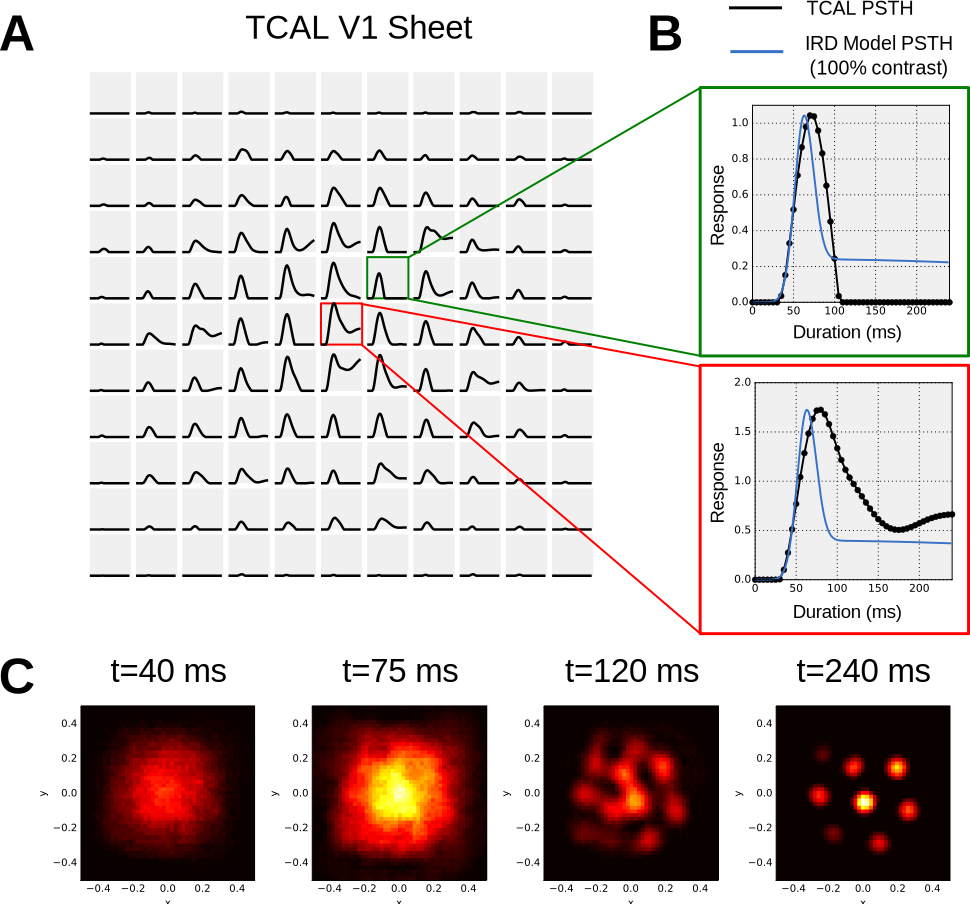
\includegraphics[width=0.95\textwidth]{./figures/TCAL_V1_PSTH.pdf}
\caption{{\bf Activity profiles of TCAL V1 sheet units at the start of
    development in response to an isotropic Gaussian stimulus pattern.}
  (A) An $11\times11$ spatially sampled grid of PSTH profiles in the V1
  sheet of the TCAL model after model initializations. (B) Two PSTH
  profiles visualized in more detail, taken from the red and blue units
  shown in (A). Blue traces show an summary of the experimental data
  using the IRD model at $100\%$ contrast
  \citep{albrecht_jneurophys02}.  The traces of the descriptive model
  are normalized to the response level of the TCAL model. The two units
  have been selected to demonstrate the initial diversity in responses
  in the TCAL model. (C) Bubble formation timecourse in TCAL, showing
  the activity over the entire V1 sheet. Between $t=40$ \si{\ms} and the
  maximum mean response at $t=75$ \si{\ms} the activity increases to a
  peak, roughly following the spatial Gaussian profile of the afferent
  input from the LGN. At $t=120$ \si{\ms}, the activity has started to
  decay and activity bubbles are starting to form. By the end of the
  simulated fixation at $t=240$ \si{\ms}, there are clear, settled
  activity bubbles.}
\label{fig:TCAL_V1_PSTH}
\end{figure}


In addition to plasticity, there is an initial diversity in the V1 PSTH
profiles that does not exist in the ON/OFF sheets. This diversity is
present before development, i.e. right after the model is initialized,
as highlighted by the two profiles selected in Figure
\ref{fig:TCAL_V1_PSTH}. The two profiles shown in the red and green
boxes have differently shapes, unlike the incoming activity from the
ON/OFF sheets that all has the same temporal profile, as shown in
Figure \ref{fig:TCAL_LGN_PSTH}.

This diversity of response profiles is a result of the initial,
randomized afferent and lateral inhibitory weights and the competitive
nature of the settling process driven by the lateral, Mexican-hat
inhibition profile, shown in Figure \ref{fig:Mexican_hat}C. When a cortical area is stimulated, the individual
units compete to represent the stimulus by suppressing their neighbors
via lateral inhibition. Together with the randomized weights, this process
breaks symmetry and leads to a corresponding diversity of activity
profiles, even for a perfectly symmetrical stimulus such as the Gaussian
input used in Figure \ref{fig:TCAL_V1_PSTH}.

Another way of viewing this diversity is to note the difference in
responses between units \emph{after} the PSTH peak, seen in Figure
\ref{fig:TCAL_V1_PSTH}C. This subfigure shows the activity of the V1
sheet at four time points within the fixation, at $40$, $75$, $120$, and
$240$ milliseconds respectively. The initial activity in V1 inherits the
Gaussian spatial profile from the ON/OFF sheets, seen in Figure
\ref{fig:TCAL_LGN_PSTH}. This broad Gaussian activity peaks in V1 and
then as the afferent input falls, lateral interactions start to dominate
and activity bubbles begin to form.

This also explains why the overall profiles of the units across space,
shown in Figure \ref{fig:TCAL_V1_PSTH}A reflect the shape of the
Gaussian input on the retina, while also supporting activity bubble
formation. The initial response that includes the peak is similar across
the entire cortical population and only later do lateral interactions
start to dominate. In other words, all the units that have afferent
drive will respond with a similarly shaped initial peak in the firing
rate, but only units that form part of an activity bubble will be
sustained. Other neurons that are strongly suppressed by lateral
inhibition will fall silent, as for the neurons initially responding
but now in dark areas between the activity bubbles.

This effect is illustrated by the two selected PSTH curves in Figure
\ref{fig:TCAL_V1_PSTH}B. Both units are near the center of the response
and both units have a clear peak in their firing-rate activity. The
firing-rate response of the unit in the green box falls to zero, while
the response of the central unit in the red box falls after the initial
but then begins to rise again as the bubble in which it is located sharpens.

One helpful way to understand this process is to suppose that the unit
marked green is being suppressed laterally by the unit marked in
red. This would happen if the green unit is outside the local excitation
field of the red unit but within its larger inhibition field. This is
simply the Mexican hat interaction that drives bubble formation (but
remember, this is only an \emph{effective} profile, not necessarily a
fully mechanistic operation). For a description of the Mexican hat
profile, see section \ref{section:self_organization_principles}.

We have now considered the dynamics of the evoked response in terms of
the PSTH profile shapes in the V1 sheet and discussed how these PSTHs
relate to activity bubble formation. Next we look at how the bulk
activity dynamics across the cortical surface may be related to the
experimental data.


\subsection{Evoked population response}

The spatial sampling of V1 response profiles shown in Figure
\ref{fig:TCAL_V1_PSTH}A is very similar to the earliest version of the
SIRD model shown in Figure \ref{fig:SIRD_calibration_sampling}B of
Chapter \ref{chapter:SIRD}. This illustrates exactly how the starting
point of the SIRD model connects with TCAL, which can then guide future
work. Using the extensive calibration embodied by the SIRD model, it is
hoped that TCAL can be made into mechanistic, developmental framework
that can also account for the spatiotemporal properties of the VSDI
response.

Interestingly, there is an obvious discrepancy between the evolution of
the spatial activity profile in TCAL, shown in Figure
\ref{fig:TCAL_V1_PSTH}C and the spatiotemporal profile of the VSD
response shown in Figure \ref{fig:sit_data}D
\citep{sit_neuron09}. Although the peak TCAL response, shown in Figure
\ref{fig:TCAL_V1_PSTH}C at $t=75$ \si{\ms} has a roughly Gaussian
spatial profile just like the VSD response shown in Figure
\ref{fig:sit_data}, TCAL's response then deviates from this initial
Gaussian profile as activity bubbles form.

Although only the peak spatial profiles of the response are shown in the
\citet{sit_neuron09} paper, it is possible to infer that the spatial
profiles are smooth throughout the response by examining the plots in
Figure \ref{fig:sit_data}D. The raw $\Delta F/F$ signal shown in Figure
\ref{fig:reynaud_data}B uses a different experimental protocol and there
is still no strong evidence that the spatial profile of the response
dramatically changes shape as activity bubbles form.

Activity-bubble dynamics are a necessary feature of a developmental map
model, and this is the first time they have been considered in the
context of the VSDI response. If activity bubbles form in animal V1,
why would they not be visible in the VSD signal?

First we will note that activity bubbles form on a similar spatial scale
to the orientation hypercolumns, as it is in fact the size of the activity bubbles
that determines the spatial scale of the map \citep{miikkulainen_2005}. By
comparing the scale bar showing the orientation hypercolumn distance in
Figure \ref{fig:example_OR_maps}B and the scale of the VSDI signal shown
in Figure \ref{fig:ST_gradient}, it is clear that the activity bubbles
shown in Figure \ref{fig:TCAL_V1_PSTH}C are not shown on the same scale
as the VSD signal.

Figure \ref{fig:TCAL_SIRD_link}A shows the spatiotemporal response
analysis of the TCAL model firing rate after the sheet area is tripled,
putting the activity bubbles on a more suitable relative spatial
scale. In part A, the firing-rate response is shown at the point when
the bubbles are not very clearly visible at the peak of the response at
$80$ \si{\ms}, clearly visible after $130$ \si{\ms} and at the end of
the fixation at $240 $\si{\ms}.

\begin{figure}
\center
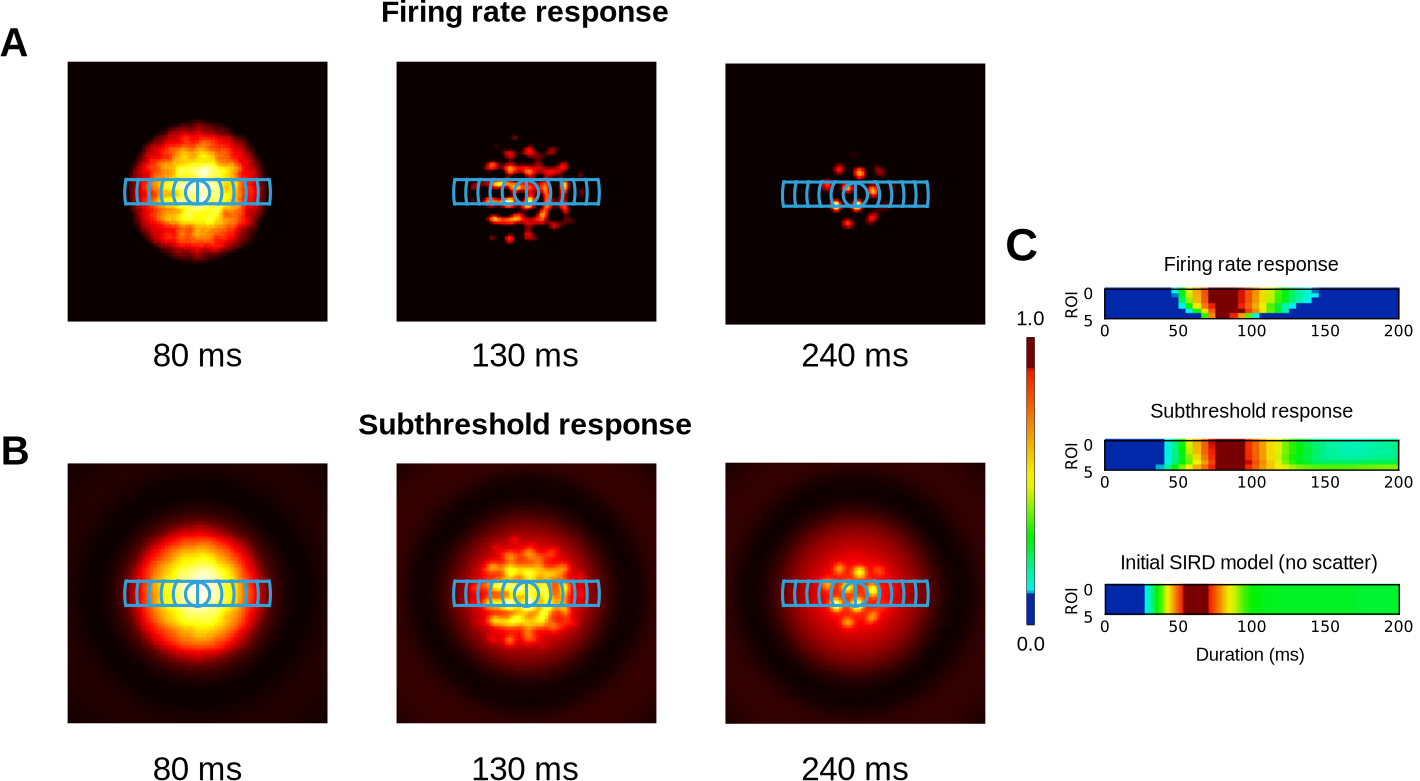
\includegraphics[width=0.95\textwidth]{./figures/TCAL_SIRD_link.pdf}
\caption{{\bf Differences between the firing-rate response and the absolute sum
    of synaptic contributions per unit.} (A) firing-rate response at
  $80$, $130$, and $240$ milliseconds after stimulus onset, showing
  where activity bubbles when they first form and at the end of the
  response. (B) Sum of absolute synaptic inputs across all projections
  in V1, weighted by the projection weights, at the same times after
  stimulus onset. (C) Corresponding spatiotemporal plots. The top plot
  shows the spatiotemporal analysis of the firing-rate response, the
  middle plot shows the spatiotemporal analysis of the subthreshold
  response and the bottom plot shows the spatiotemporal analysis at an
  early stage of the SIRD model, replicating Figure
  \ref{fig:SIRD_calibration_sampling}D. Note that there is still a
  response continuing to $240$ milliseconds in the firing response as seen in (A)
  but it is not visible in (C) because of clipping of low values
  caused by this particular color map. }
\label{fig:TCAL_SIRD_link}
\end{figure}


The top spatiotemporal plot Figure \ref{fig:TCAL_SIRD_link}C illustrates
how activity bubble formation results in a non-smooth spatiotemporal
response in terms of the cortical firing rate, even after having
rescaled the cortical sheet. Both the spatial profile at peak and the
spatiotemporal plots are unlike those of the real VSD signal, as shown
in Figure \ref{fig:ST_gradient}.

I.e., rather than the smooth Gaussian-like activity seen in Figure
\ref{fig:SIRD_calibration_sampling} of the SIRD model, TCAL suggests
that the underlying activity pattern will be patchy.  This result is
not incompatible with the SIRD model, because spatial isotropy in that model
was imposed directly from the observed spatial profile of the VSD
signal, explicitly ignoring any smaller scale spatial modulation. What
does demand explanation is why the spatial profile of a developmental
model diverges so clearly from the observed properties of the VSD signal.

In TCAL, as in GCAL before it, the firing rate is approximated by
applying a firing threshold to a subthreshold contribution, summed over
the various types of projection to each unit. If this firing threshold
value is ignored, the subthreshold activity can be loosely thought of as
the membrane voltage. By considering the subthreshold contribution from
each projection to a V1 unit (two afferent projections from the ON/OFF
sheets as well as the lateral excitatory and lateral inhibitory
projections) it is possible to try to relate the model more closely to
the VSD signal than by using firing rates.

As discussed in Section \ref{section:VSDI_background}, the VSD signal
is generated by a voltage-sensitive--dye that binds to cell membrane
and reflects voltage changes, not spiking. This signal reflects both
excitatory and inhibitory activity, such that more inhibition will
\emph{increase} the VSD signal, even though it reduces the firing
rate.  This is a very important consideration, because the activity
bubbles in GCAL and TCAL develop by inhibition of an initially broader
pattern of activity that leads to inactive units between the active
bubbles. 

The simplest way to model the VSD signal in TCAL is to take the projection
activities that correspond to the synaptic contribution, take the
absolute value so both excitatory and inhibitory projections contribute
positively, and sum these different contributions up, as weighted by the
projection strengths in the model. The result of applying this operation
is shown in Figure \ref{fig:TCAL_SIRD_link}B.

Now the activity bubbles have a greatly reduced impact on the signal,
even though they are still present at the firing rate level as in Figure
\ref{fig:TCAL_SIRD_link}A. Unlike the firing response, which can fall to
zero as activity falls below the firing rate threshold, the subthreshold
response is present across the entire spatial area for the duration of
the evoked response. The corresponding spatiotemporal analysis is shown
in the middle plot of Figure \ref{fig:TCAL_SIRD_link}C.

There is now a good qualitative match with the bottom plot of Figure
\ref{fig:TCAL_SIRD_link}C which shows the top plot of Figure
\ref{fig:SIRD_calibration_sampling}D. In other words, the responses in
TCAL behave like the earliest stages of the SIRD model, before latency
scatter was introduced.

The match is not exact as the TCAL-neuron onsets do not quite align, and TCAL has a
slightly greater time constant. Both these issues could be improved with
additional parameter tuning and the match is certainly close enough to
use the SIRD model as a guide to future work on TCAL. Note that the
increased time constant may be partially due to the slightly slower
response of TCAL units relative to the IRD model, as shown in Figure
\ref{fig:TCAL_V1_PSTH}B, but it could also be partly due to averaging the
responses in Figure \ref{fig:TCAL_V1_PSTH}A which are not all identical.

Improving TCAL's VSD signal model, parameter tuning, and investigating
how to introduce the various forms of diversity motivated by the SIRD
model are all items for future work, discussed in section
\ref{section:future_work}. There is one way that TCAL now make an
advance on the SIRD model which is to introduce a real diversity of
tuning, taking a step towards explaining the tuning-dependent latency
variance term, $\pmb{\tau}_T$. This has not yet been shown in TCAL as we
have only examined the initial state of the model. To consider tuning,
we need the TCAL units to acquire tuning properties and for that, we now
need to consider development.

\subsection{Orientation map development}

Having made significant changes to the activity dynamics in order to
calibrate single-unit responses, it would not be surprising if TCAL was
no longer able to function as a developmental map model like GCAL and
CGCAL. The bubble formation seen towards the end of a fixation period,
shown in Figure \ref{fig:TCAL_V1_PSTH}C, does suggest that the map
formation process may still operate but it is impossible to establish
this without running a developmental simulation.

In this section we see that TCAL is still a developmental map model,
although one particular discontinuity that CGCAL eliminated from GCAL will
be reintroduced for expediency, because certain properties of the evoked
response interfere with the development process.

\subsubsection*{Learning driven by activity bubbles}
\label{section:TCAL_snapshot_learning}

Figure \ref{fig:TCAL_No_Snapshot} shows the TCAL orientation preference
and selectivity maps after $18000$ presentations. The orientation maps
are measured in the full model at $240$ milliseconds after the onset of
the sinusoidal gratings used to measure the orientation response. This
approach in the full model is more comparable to what would be measured
in the animal than the analysis in Chapter \ref{chapter:GCAL}, which was
designed to reveal the afferent component of the orientation preferences
to allow easier comparison between models. In all other aspects, the
measurement protocol remains the same.

It is clear that although the orientation preferences, selectivities, and
afferent weights have changed over development, the overall map
organization and weight development is poor. This is most clearly
illustrated by the lack of organization of the weights shown in Figure
\ref{fig:TCAL_No_Snapshot}C, which are smooth but appear largely unselective.

\begin{figure}
\center
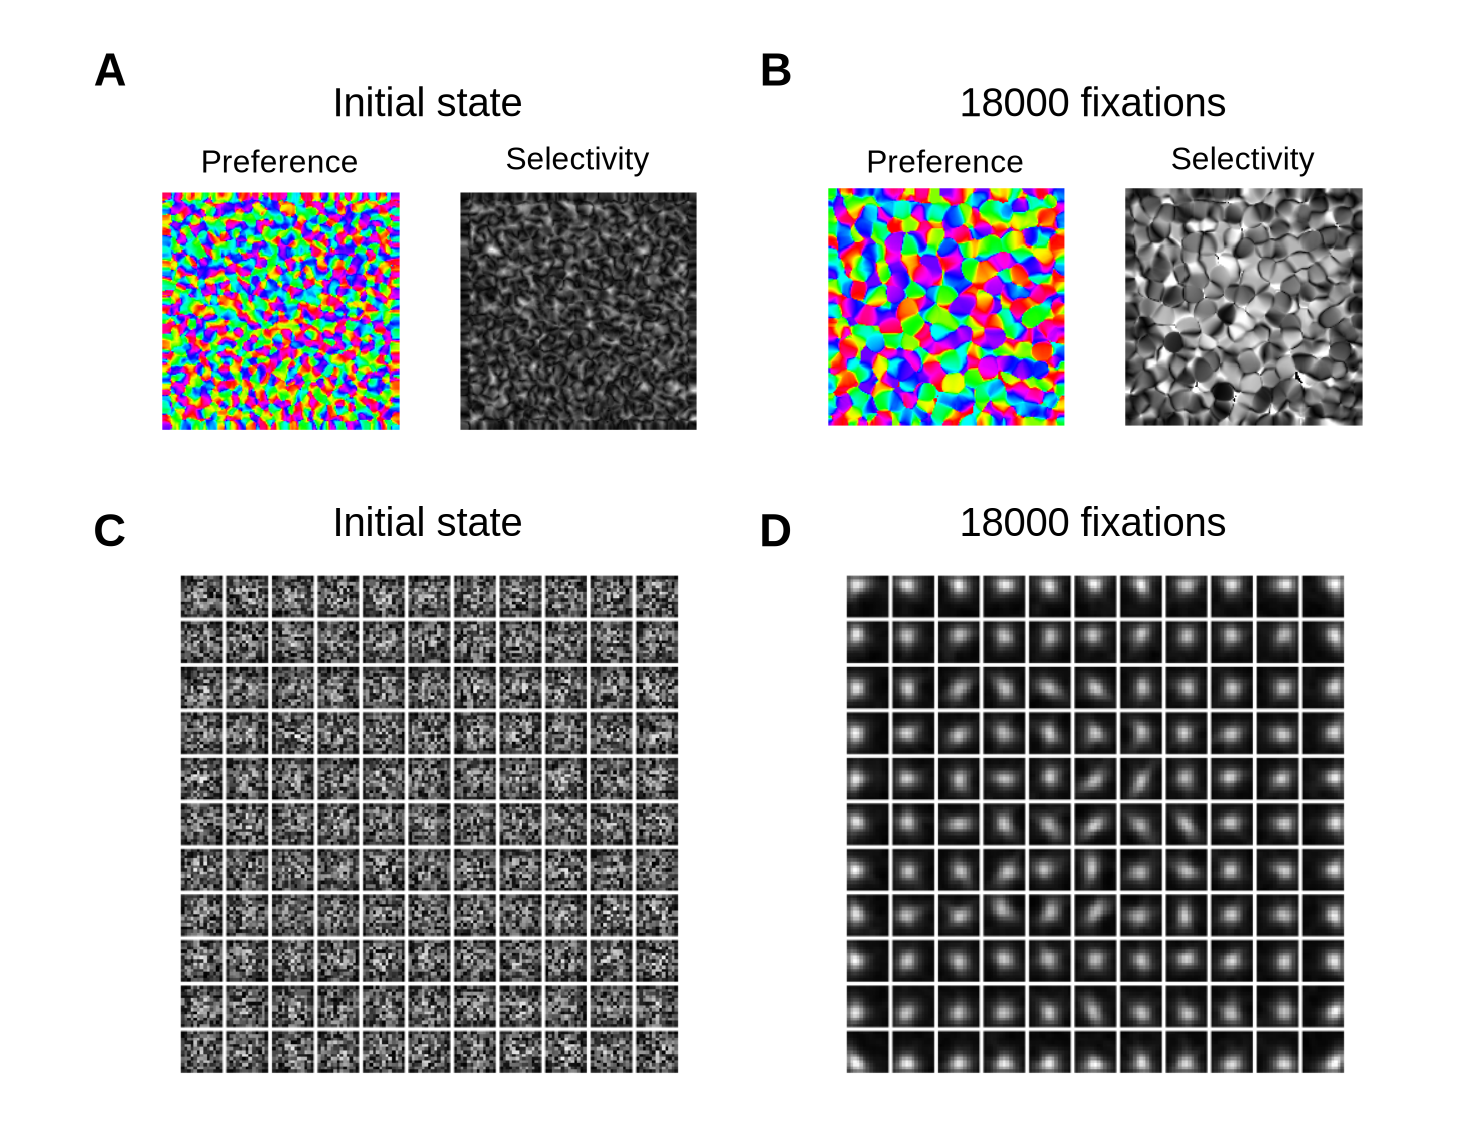
\includegraphics[width=1.1\textwidth]{./figures/TCAL_OR_No_Snapshot.pdf}
\caption{{\bf Development of orientation maps and afferent weights in
    TCAL with continuous learning} (A) Orientation selectivity
  and preference map of the full model after initialization. The
  apparent structure in the preference map is due to the Mexican hat interactions
  in an unorganized network, as illustrated in Figure
  \ref{fig:Mexican_hat}C, causing bubbles to form but not in any
  reliable way.  (B) Corresponding map measurements after
  simulating 18000 fixations. The map structure is poor overall, with sharp
  discontinuities, but some neurons are highly selective. (C)
  Afferent weights from the ON sheet to the V1 sheet for an $11\times11$
  regular sampling of units after initialization. The random initial
  state of the network is visible. (D) The same afferent weights from
  the ON sheet after 18000 fixations. The weights are now smooth but
  only a few of the neurons have become selective.}
\label{fig:TCAL_No_Snapshot}
\end{figure}

Given that TCAL was calibrated only to have realistic PSTH profiles in the
ON/OFF and cortical sheets, it is unsurprising that development has
failed to proceed in a plausible way given how radically the activity profiles
have been modified. The question now is whether plausible
development can be recovered without losing the calibrated firing
response profiles.

When discussing Figure \ref{fig:TCAL_V1_PSTH}C, the presence of the
activity bubbles necessary for proper map development was identified but
it was also noted that this settling only occurred after an unselective
bloom of activity driven by the initial activity to reach the cortical
sheet. With continuous learning, the high activity during this bloom
will have a large effect on the synaptic weights, as opposed to the
activity bubbles that have a much lower activity and form later on in
the response.

This suggests a possible way to recover development by introducing one of the
mechanisms that was eliminated to make CGCAL into a model without
temporal discontinuities. If snapshot learning were reintroduced at the
point where activity bubbles have formed, perhaps the developmental
process can be recovered without sacrificing the earlier PSTH
calibration?

Figure \ref{fig:TCAL_Snapshot} shows that this is indeed possible. With
snapshot learning triggered at $130$ milliseconds into the response of
each fixation, the orientation map structure after $18000$ iterations
looks far more plausible. Even more convincingly, the weight structure
shows plausible organization even though these weights were noisy. Note
that with snapshot learning reactivated, the learning rates once again
match those of the GCAL model exactly, instead being divided by a factor
of $20$ as they were when continuous learning was applied.


\begin{figure}
\center
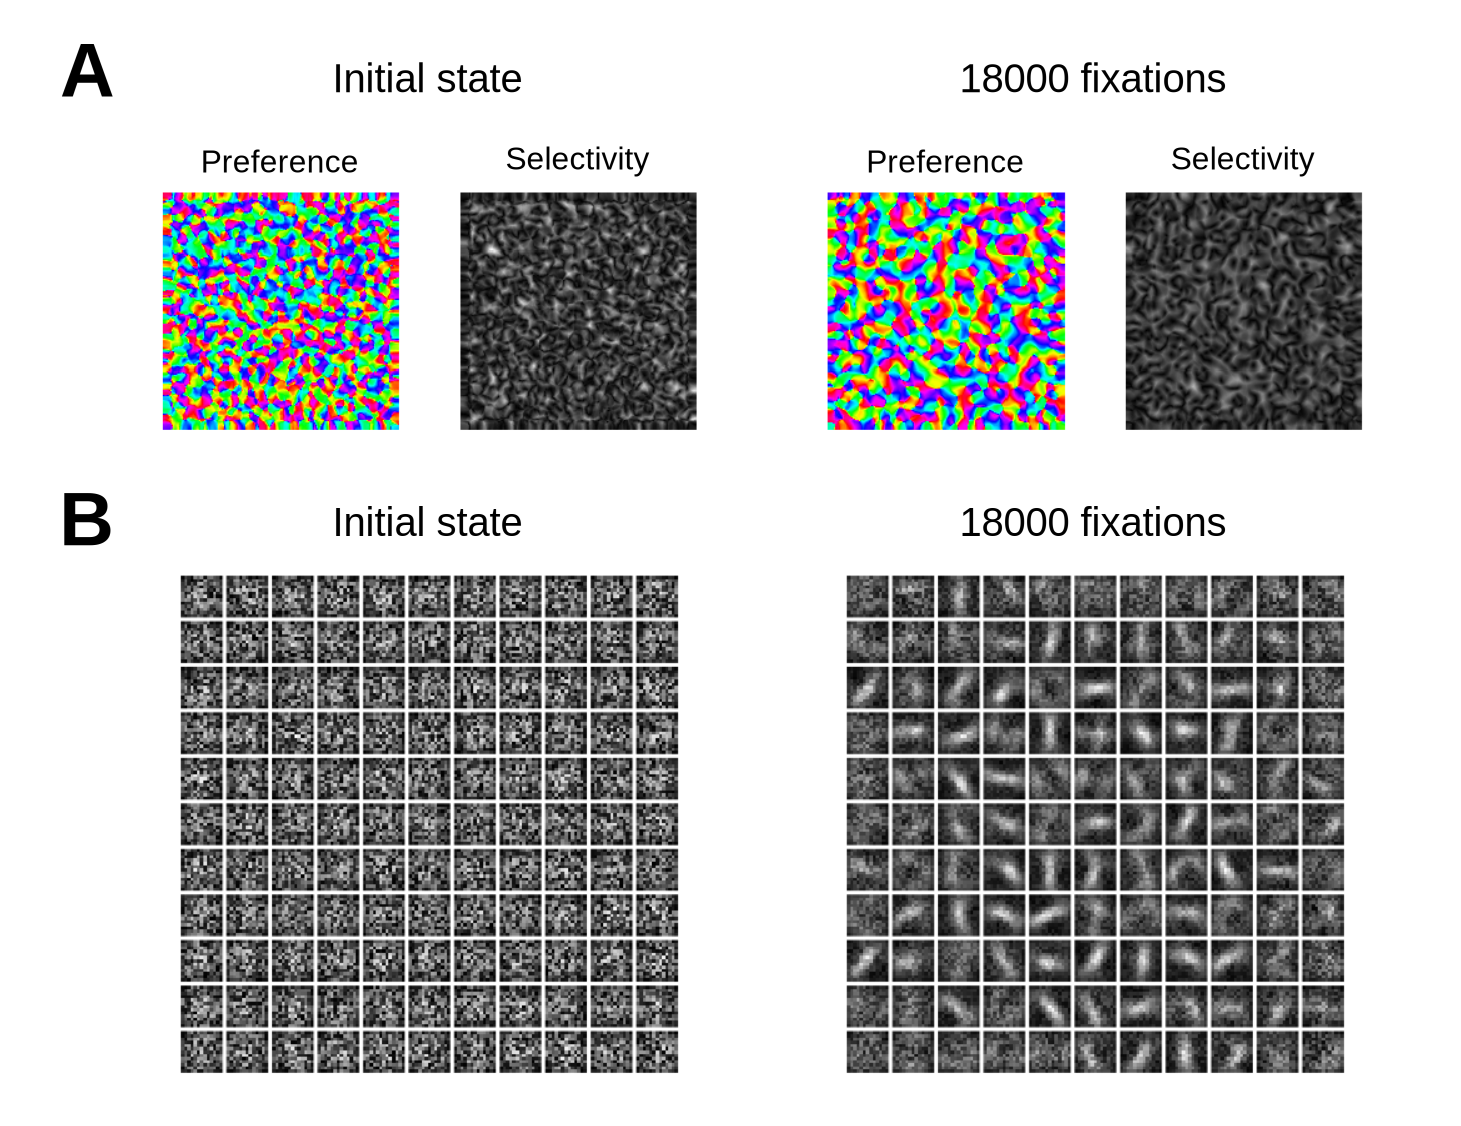
\includegraphics[width=1\textwidth]{./figures/TCAL_OR_Snapshot.pdf}
\caption{{\bf Development of orientation maps and afferent weights in
    the TCAL model with snapshot learning after $130$ milliseconds} (A)
  Orientation selectivity and preference map of the full model after
  initialization. As the same initial random seed was used as in the
  previous figure, these maps are identical to those in Figure
  \ref{fig:TCAL_No_Snapshot}A. (B) Corresponding map measurements after
  simulating 18000 fixations. The map structure is now much more
  realistic than before although selectivity is poor. (C) Afferent weights
  from the ON sheet to the V1 sheet upon model initialization that
  matches those in Figure \ref{fig:TCAL_No_Snapshot}C due to the use of
  an identical random seed. (D) The afferent weights from the ON sheet
  after 18000 fixations. The weights are still noisy, suggesting the
  learning rate could be increased, but now there is evidence of proper
  organization of the afferent weight structure.}
\label{fig:TCAL_Snapshot}
\end{figure}

As argued in Chapter \ref{chapter:GCAL}, presenting a few orientation
maps as in Figures \ref{fig:TCAL_No_Snapshot} and
\ref{fig:TCAL_Snapshot} does not make for a convincing analysis. In that
chapter, a quantitative approach was presented to assess developmental
models of orientation map formation. It now makes sense to use that
approach for comparing development in the TCAL model with and without
snapshot learning.

Figure \ref{fig:TCAL_Snapshot_analysis} shows the results of this
analysis using ten simulations for $18000$ training presentations using
ten different random seeds to control weight initialization and training
sequence. The mean map quality, selectivity, and stability metrics
described in Chapter \ref{chapter:GCAL} are shown, including the
standard error from the mean. In A, the results are shown using
continuous learning while in B the results are shown for snapshot
learning after $130$ milliseconds.

\begin{figure}
\center
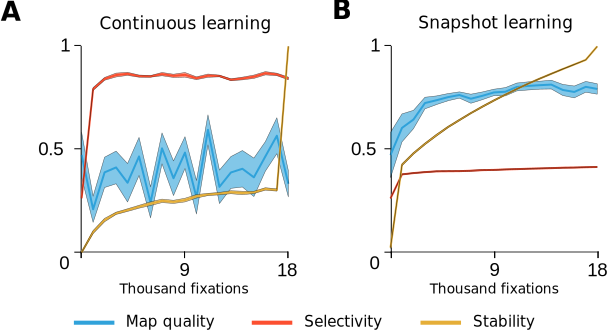
\includegraphics[width=0.8\textwidth]{./figures/TCAL_Snapshot_OR_analysis.pdf}
\caption{{\bf Analysis of ten different randomized TCAL simulation runs
    over $18$ thousand training presentations with and without
    continuous learning. Metrics shown are map quality, selectivity, and
    stability.}  Maps were simulated with a $2.0\times2.0$ area that was
  cropped to a $1.75\times1.75$ area to reduce border effects. Solid
  lines indicate the mean values and the surrounding area indicates one
  standard error deviation from the mean. (A) Map quality, selectivity,
  and stability using continuous learning. Selectivity grows quickly but
  the map quality metric indicates no proper map organization and
  stability is very poor. (B) Map quality, selectivity, and stability
  using snapshot learning after $130$ milliseconds. Selectivity is now
  lower but both the stability and the map metric values have
  improved. Note that the average Hebbian learning rates match those of
  the GCAL model, with the continuous learning rates rescaled
  appropriately.}
\label{fig:TCAL_Snapshot_analysis}
\end{figure}

The results confirm the analysis shown in Figures
\ref{fig:TCAL_No_Snapshot} and \ref{fig:TCAL_Snapshot}, showing that
snapshot learning helps development proceed more quickly and reliably,
reaching a greater level of organization within the simulated time period.
With snapshot learning, the
stability and the map quality metric are greatly improved. Although the
map metric is still not as good as GCAL's perfect $\pi$
pinwheel density, the way the metric increases over development
demonstrates that the same self-organization process is at work in TCAL.

The results shown in Figures \ref{fig:TCAL_Snapshot} and
\ref{fig:TCAL_Snapshot_analysis} are remarkable when considering the
ways TCAL is both different from and similar to GCAL: (1) Unlike GCAL,
TCAL has calibrated firing rate profiles in the LGN and V1 sheets, which
now have a very different shape. (2) Only
one additional parameter is needed, namely the hysteresis time constant
in the ON/OFF sheets. (3) The only modified parameters in the ON/OFF sheet
are the strength of the contrast-gain control mechanism and its delay. (4)
All parameter values are equivalent to those in GCAL except for the
afferent projection strength to V1, which has been boosted by a factor of
five to compensate for reduced activity in the LGN.

Additionally, it is likely that the map quality could be further
improved by either increasing the number of training steps or boosting
the learning rate, in order to get rid of the noise in the weights shown
in Figure \ref{fig:TCAL_Snapshot}B after development. It is clear that
with additional parameter tuning and training iterations, it will be
possible to improve both the PSTH calibration and orientation map
development in TCAL simultaneously.

What is not clear is whether the re-introduction of snapshot learning has
some biological justification, or whether it is indeed necessary. It
is possible that a constant, 
continuous learning rate simply means map development occurs much more
slowly, due to the way the activity bubble response is dwarfed by the
initial unspecific response. Alternatively, the snapshot learning
mechanism could be replaced by a continuous mechanism that modifies the
learning process. For instance, perhaps learning is quicker when the
network is quiescent or approaches a stable steady state, or there are some
other mechanisms that result in reduced learning of the initial
unspecific response.  Investigating the ways snapshot learning can be
eliminated in favor of a continuous mechanism and finding the
corresponding biological justification (if any) is a topic for future
work, discussed in section \ref{section:future_TCAL_snapshot_learning}.


\section{Bridging timescales}
\label{section:bridging_timescales}

Figure \ref{fig:TCAL_Conclusion} shows how TCAL bridges the timescale of
development with the timescale of the evoked response within a single,
unified model. All the results shown in this figure are drawn from the
same map simulation shown in the previous figure. As a result, A, B, and C
match the results shown in Figure \ref{fig:TCAL_Snapshot}A after zero
and $18000$ training iterations.  In addition, Figure
\ref{fig:TCAL_Conclusion} shows the same results at two intermediate
stages of the simulation run, after $6000$ and $12000$ iterations
respectively.

\begin{figure}
\vspace*{-3ex}%
\center
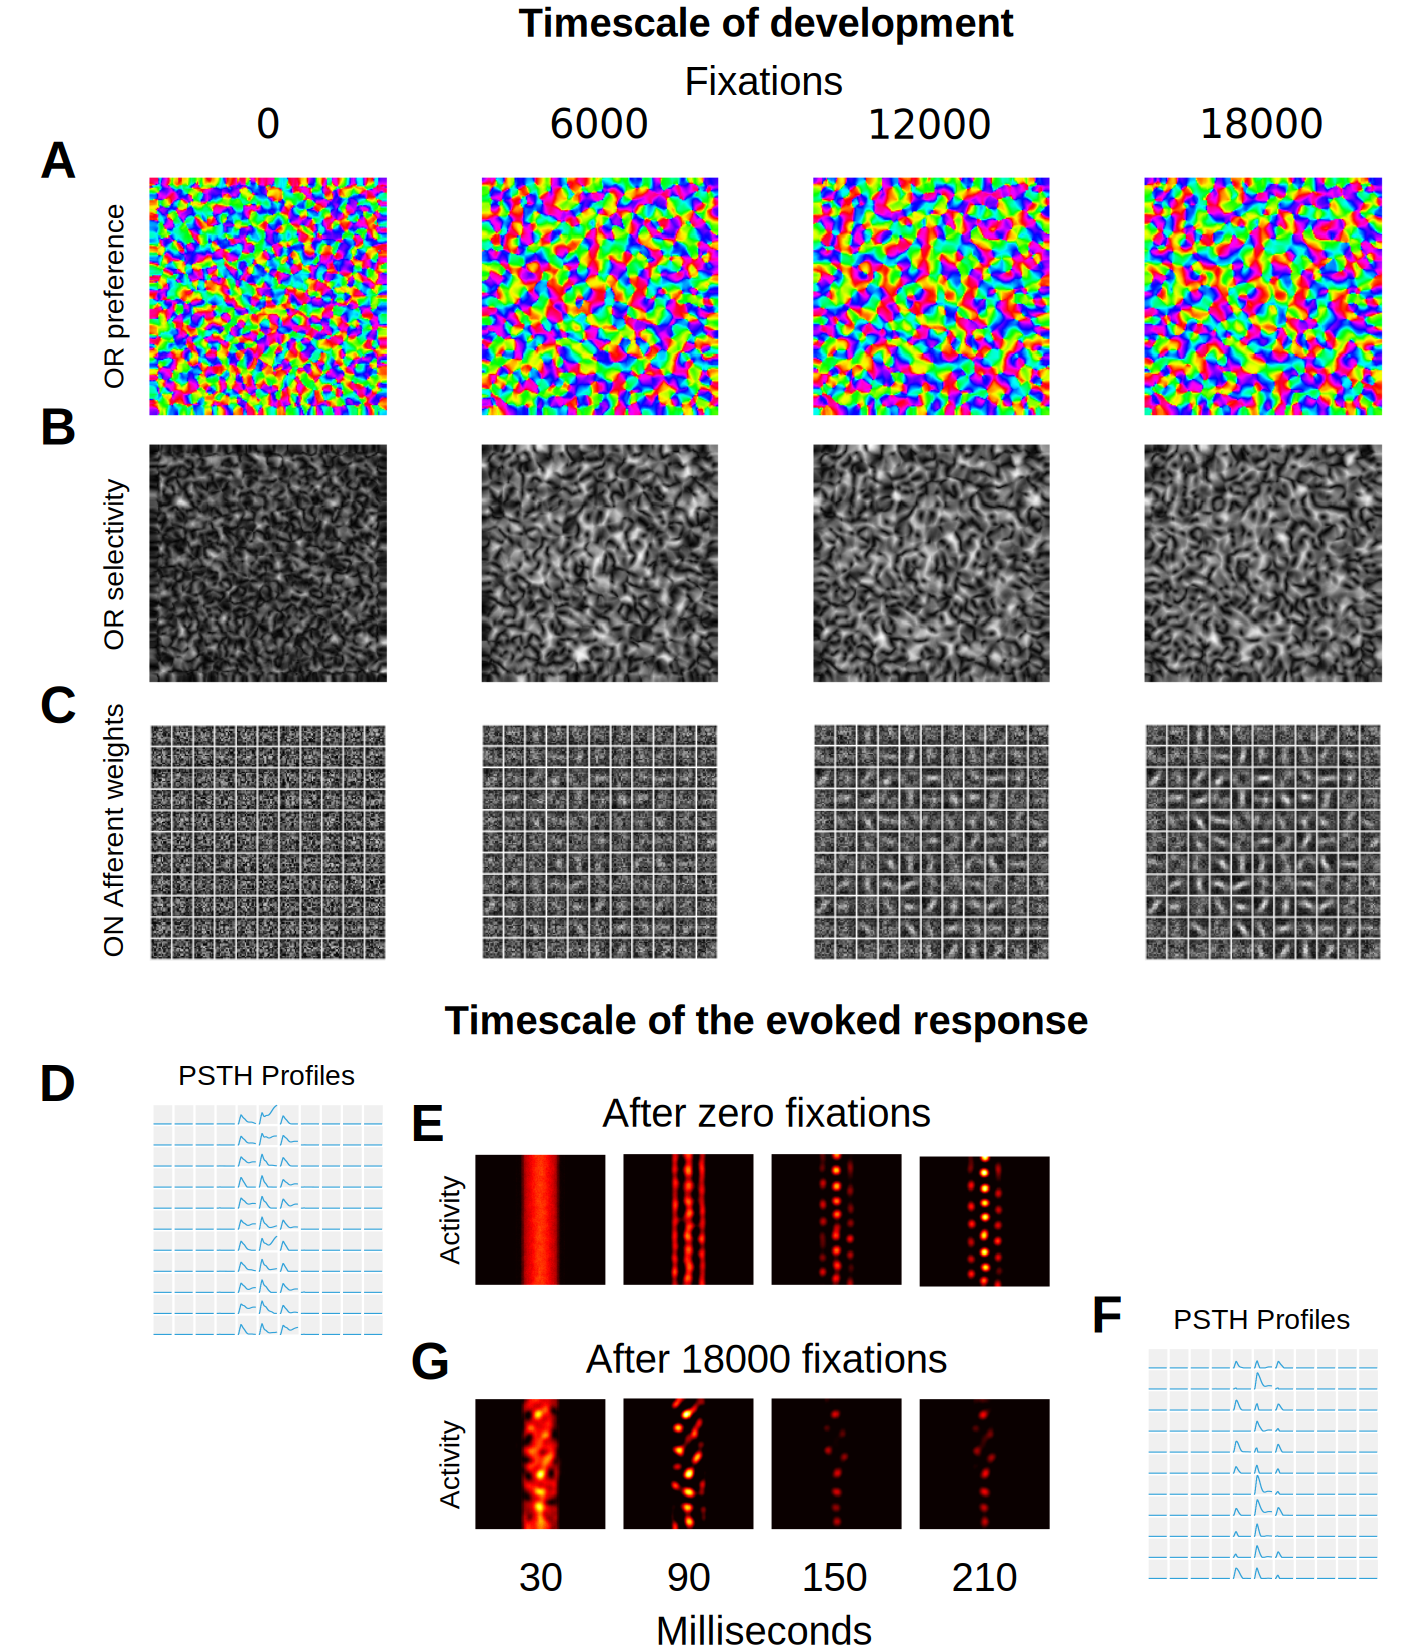
\includegraphics[width=0.95\textwidth]{./figures/TCAL_Conclusion.pdf}
\caption{{\bf Illustration of how the TCAL models bridges across
    temporal scales} (A) Orientation preference maps recorded after
  zero, $6000$, $12000$, and $18000$ fixations. (B) Corresponding
  orientation selectivity maps. (C) Afferent weights from the ON sheet
  for a regularly sampled $11\times11$ selection of neurons in the V1
  sheet. After $18000$ fixations, there is self-organization from the
  random initial weights shown at fixation zero. (D) Corresponding PSTH
  profiles for the same $11\times11$ sampled units in response
  to a vertical line stimulus after zero training fixations. Each PSTH
  response is measured for a $240$ millisecond duration, corresponding
  to the duration of a fixation (E) Activity response of the entire V1
  sheet at $30$, $90$, $150$, and $210$ milliseconds in response to the
  vertical line stimulus. (F) Corresponding PSTH profiles for the same
  $11\times11$ units after $18000$ training fixations. Note that the
  PSTH profiles have changed due to the developmental process and that
  the responses are now more diverse. (G) Activity of the V1 sheet to
  the same vertical line stimulus after $18000$ training iterations,
  shown at the same time points in the evoked response. The activity
  bubbles at the end of the response now reflect areas that are
  selective to the vertical orientation, and the dark areas in between
  represent areas selective for other orientations.}
\label{fig:TCAL_Conclusion}
\end{figure}


In Figure \ref{fig:TCAL_Conclusion}D, we observe the evoked response
before training in response to a vertical line stimulus, for exactly the
same regular sampling of units used throughout this figure and shown in
Figure \ref{fig:TCAL_Snapshot_analysis}B. The response is initially unselective as
the network has not been trained. Figure \ref{fig:TCAL_Conclusion}E
shows the activity of the entire V1 sheet at four different times,
illustrating clearly the initial unselective bloom after $30$
milliseconds and the subsequent activity bubble formation. By $210$
milliseconds, a fairly regular array of activity bubbles has formed.

In Figure \ref{fig:TCAL_Conclusion}F and G shows the corresponding
measurements of the evoked activity at the end of the developmental run,
after $18000$ training pattern presentation or fixations. The evoked
response properties as sampled over $240$ milliseconds and shown in F
are now different from the responses shown in D. This is because the
weights have now self-organized through Hebbian learning and the units
have now become orientation selective, and have structured receptive
fields as evidenced by the afferent weight structure at the
corresponding developmental point shown in C. This difference in
response also reflects the tuning of the units, as vertically selective
units will be most strongly driven by this vertical line stimulus.

The effect of development on the evoked response can also be seen in G,
which shows the activity of the V1 sheet in response to the same
stimulus and at the same time points shown in E. The regular bubble
position and overall uniformity of the response present before
training no longer applies. Once again, this is due to the diverse
tuning properties of the V1 units that have emerged over the course
of development.

The difference between Figures \ref{fig:TCAL_Conclusion}D and F
illustrates the core idea of this thesis. Both are examples of evoked
responses to a visual stimulus, of the sort that might be recorded
experimentally with an electrode array. As such experimental recordings
are typically performed in the adult animal, an experimenter is
likely to observe a diversity of responses and tuning properties, as
shown in Figures \ref{fig:TCAL_Conclusion}F.  These models predict
that this diversity reflects the long-term relationship between these
neurons and their visual environment, encoded in a pattern of weights
and network structure that determines how the neurons will respond to
a new stimulus.

\section{Discussion}

What is unique about the TCAL model is in the particular way it accounts
for this diversity of evoked responses and tuning properties in the
evoked response. Activity is computed per unit by integrating neural
activity projected through weight fields such as those shown in Figures
\ref{fig:TCAL_Conclusion}C. These weight fields are not imposed by
attempting a direct calibration with experimentally determined
connectivity profiles recorded from adult animals. Instead, they are
self-organized through a developmental process, driven by tens of
thousands of visually evoked responses during training.

Other than the re-introduction of the snapshot learning process, TCAL is
a continuous model. This means every simulation timestep follows the
same rules, computing activity responses and very gradually shaping the
network structure through Hebbian learning. In this way, the difference
in the evoked response shown in Figure \ref{fig:TCAL_Conclusion}D and
Figure \ref{fig:TCAL_Conclusion}F is a reflection of the $18000$ evoked
responses that occurred during training that separates these two states
of the model. As the statistics of the training patterns used will
affect the development of the network, we can now see how TCAL meets the
stated aims of this thesis, listed at the start of Section
\ref{section:Aims}.

To recapitulate these aims, expressed in terms of what the TCAL model
achieves: (1) Each V1 unit responds in the context of a surrounding
population to which it is connected. (2) The history of evoked
responses, starting from the initial conditions explains how this
specific pattern of connectivity arises. (3) This history of evoked
activity is driven by visual input to the model, and so the
connectivity of the model reflects the long-term statistics of the
visual environment.

In addition to showing a concrete example of how the stated goals of
this thesis were achieved, Figure \ref{fig:TCAL_Conclusion} shows how
TCAL is connected to the work in two of the previous chapters. Only the
analysis developed in Chapter \ref{chapter:GCAL} with respect to the
pinwheel density map metric is not shown, as this was demonstrated in
Figure \ref{fig:TCAL_Snapshot_analysis}.

The first link is with Chapter \ref{chapter:reproducible_workflow}, as
the results shown in this figure were taken from one of ten different
simulation runs analyzed in Figure \ref{fig:TCAL_Snapshot_analysis},
launched with Lancet and visualized with HoloViews. HoloViews generated
these plots and allowed interactive exploration of all the results
across all the simulation runs, before they had even completed execution
on the compute cluster.

This figure then connects with the work in Chapter \ref{chapter:SIRD}, as
subfigures D and F show regularly sampled PSTH profiles across space in
a very similar way to those presented at the start of the SIRD model,
shown in Figure \ref{fig:SIRD_calibration_sampling}B. The VSD signal
model shown in \ref{fig:TCAL_SIRD_link} could also have been applied to
the responses shown in subfigures E and G. This would have allowed the
same spatiotemporal analysis and plots to be generated as used
throughout Chapter \ref{chapter:SIRD}. These plots would show the
response to a vertical line stimulus and not a Gabor path and the
responses shown would have been computed by a mechanistic, developmental
model.

\section{Conclusion}

TCAL is a mechanistic, developmental model that connects developmental
processes to the evoked response. It features calibrated firing rate
profiles in both the subcortical and cortical sheets. In the subcortical
sheets, calibration is done with respect to experimentally derived PSTH
profiles and in the V1 sheets, calibration is done using by the IRD
model which is also the basis of the SIRD model presented in Chapter
\ref{chapter:SIRD}. TCAL also feature developmental self-organization
including the formation of smooth orientation maps and the emergence of
varied tuning properties across the cortical population.

All this is achieved by the introducing a single hysteresis time
constant and very simple damping mechanism to the basic structure of the
GCAL model that precedes it. This addition is counteracted by the
elimination of various discontinuities in temporal processing of the
GCAL model, making the final definition of TCAL conceptually and mathe
atically simpler than that of GCAL, though it does take much longer to
simulate.

The result is a unified, mechanistic model that computes cortical
activity in response to a stimulus using a firing rate representation.
These evoked properties make contact with firing rate data and all the
experimental calibration embodied by the SIRD model, presented in
Chapter \ref{chapter:SIRD}.

Using Hebbian learning, this evoked activity gradually shapes the
connectivity of the network, starting from a random initial
condition. This results in a model of development that can be analyzed
using the techniques presented in Chapter \ref{chapter:GCAL}.

These results shows how TCAL allows two different experimental literatures to be
unified into a single model. In particular, all the evoked
response literature described in Section \ref{section:evoked_background}
can be used to calibrate TCAL, and so can all the developmental literature
described in \ref{section:development_background}. The result is a
unified model across spatial and temporal scales that can serve as a new
platform for future research.

\chapter{Discussion}
\label{chapter:Discussion}

The goal of this thesis is to build a single, unified model that
can account for the evoked response of an extended population of
cortical neurons in the primary visual cortex, over developmental
timescales and with millisecond resolution. In this framework, the
evoked response is computed in a network that is shaped by the entire
history of visual input. This unified approach is designed to preserve
the reciprocal link between activity dynamics and the gradual,
developmental changes to the network structure over time.

The contributions and implications of the work presented in each results
chapter will be now discussed, followed by suggestions for future work.
A wide breadth of topics and models has been covered in this thesis and
the aim of this chapter is to highlight the links between them, showing
that the total contribution of this work is more than the sum of its
parts.

Each chapter has tackled a different scientific problem that is independently
meaningful, and indeed each chapter has been published or will be published
independently.  Yet when taken together, this work points to a
new modeling approach that allows activity dynamics and self-organized
neural structure to be unified within a single, consistent framework.



\section{Firing-rate and spiking models} %% Implications

Throughout this project, the activity of cortical neurons has been
modeled at the firing-rate level, ignoring the more detailed biophysics
that can be achieved by spiking, compartmental approaches. The
trade-offs between these two representations of neural activity will be
discussed in the context of the SIRD and TCAL models.

First the SIRD model was introduced, using firing-rate units to link the
single-unit responses to the population response. In this instance,
representing activity with firing rates was appropriate because (1)
the great majority of the available experimental data that can be used
for calibration has been reported at the firing-rate level, such as
the PSTH profiles captured by the
IRD model, (2) detailed cellular biophysics would not have been a
sensible match to the other simplifying assumptions in the model
regarding the form of population level dynamics and applicable diversity
of temporal responses, and (3) a firing-rate simplification makes it far
less computationally expensive to simulate a large population of units
to correspond to the V1 area observed in VSDI studies.

This is not to say that spiking models do not have a useful
role to play. The latency scatter mechanism in the SIRD model was partly
inspired by previous work on the VSDI signal that used spiking
compartmental model \citep{chemla_neuroimage10}. It is worth considering
what benefits there would be if this kind of spiking, compartmental
model were expanded spatially in order to simulate several square
millimeters of cortical area.

Firstly, it would be possible to identify and quantify the detailed,
mechanistic contribution made by various processes to each form of
temporal diversity identified by the SIRD model. For instance, latency
scatter could be explained for in terms of varying axonal lengths,
differences in the propagation speed of action potentials, laminar
differences and delays, as well as the biophysical processes within the
individual cells. In addition, it would be possible to introduce a
realistic diversity of cell types with different temporal profiles such
as regular spiking, fast-spiking, or bursting behaviors.

If properly calibrated and constrained, such a model would directly
account for all the forms of temporal response diversity introduced by
the SIRD model, expressed in terms of biophysical
mechanisms. Unfortunately, it is not feasible to run such a large model
without consuming significant supercomputing resources. Even if the
necessary computational power were available, there is currently
far too little experimental data suitable for constraining all the
necessary biophysical parameters.

By adopting a firing-rate representation, the SIRD model loses
biophysical detail, but becomes far more convenient to simulate on
available computers and using available experimental results as constraints. 
In addition, SIRD is expressed in a very simple way that makes it
easier to understand and systematically analyze each hypothesized contribution to the
VSDI signal. A detailed spiking equivalent to this model could explain
the origin of the experimental data that was used to calibrate the SIRD
model, but only in terms of a greater number of more fundamental biophysical constants.

Using firing-rate units also allows the SIRD model to connect to other models
using a similarly simplified representation of neural activity. As the
activity state of each unit is expressed by a floating point number, a
firing rate model like the SIRD model can be easily be related to other
firing-rate models such as TCAL. If a detailed compartmental model were
used, it would be more difficult to bridge across models, because each cell
would have a complex state, defined by dozens of biophysical
variables. Ensuring two detailed models mesh together in a consistent way
is likely to pose a greater challenge than when the firing rate
representation is used.

The immediate reason that TCAL uses firing-rate units is historical,
because TCAL inherits nearly all of its structure from the GCAL
model. Like nearly all such developmental models, GCAL is based on
firing rates, so that it can simulate long timescales. Not only
is an individual spike unlikely to be an important event on long
developmental timescales, the computational cost of running a detailed,
developmental model at the spiking level would be prohibitive.

What the TCAL model shows is that it is possible to express additional,
biologically relevant information using the firing-rate units of a
developmental model without requiring a huge increase in complexity or
sacrificing the process of gradual self organization. The purpose of
TCAL is to increase the temporal resolution to the limit where the
firing-rate representation begins to break down.

By definition, TCAL does not represent the individual spikes that would be 
recorded in an experimental setup, but it still can make direct contact with
experimental data every time experimentalists choose to use a firing-rate
approximation. This simplification happens frequently, as it is difficult to
express a large number of precise spike timings in a publication, due to
the volume of data involved.  Whenever a experimenter needs to
summarize average spiking activity, for instance by computing a PSTH and
selecting an appropriate temporal bin size for the spikes, it should be
possible use this data to calibrate a firing-rate model like TCAL.

There are a few downsides with how the firing-rate units of TCAL are
implemented, and in particular when it comes to expressing the various types of temporal
diversity identified by the SIRD model. TCAL inherits its structure from
GCAL and is also implemented in the Topographica simulator, used
to simulate the development of neural sheets of firing rate units. Each
sheet defines a population of neurons and connections, known as
projections, propagate activity between them. This architecture is well
optimized for simulations such as GCAL, because it exploits
similarities between all the units in a projection, but it does make
it more difficult to add diversity, such as distance-dependent lateral
connection delays within a single projection.  Modeling these effects is
of course not impossible in Topographica, but it is less efficient and
more difficult to set up.  Some workarounds for these difficulties are
suggested as future work items in sections
\ref{section:future_distance_dependent} and 
\ref{section:future_TCAL_temporal_diversity}.


\section{Building a unified model}

In any unification, connections need to be established between different
threads that initially appear unrelated. On the surface, each of the
following topics tackle different problems in neuroscience: (1)
establishing a reproducible workflow that is flexible and allows easy
exploration, (2) relating single-unit electrode recordings to the
voltage-sensitive--dye response, (3) automatically assessing the
plausibility of developmental simulations of orientation map formation,
and (4) achieving plausible PSTH profiles in a developmental model. This
section shows how these threads connect together.

Each of these research threads address separate aspects of one
underlying problem, which is to construct a cortical model that is
unified across spatial and temporal scales. In this section, the
relationship between these research topics will be discussed and
summarized to show how these different ideas fit together.

Taken as a whole, this thesis is not intended to be an endpoint to any
particular line of research, but is instead intended to open up new avenues for
exploration. A model that can operate on developmental timescales with
plausible activity dynamics will enable more effective exploration of an
entire class of research questions. Previously, such questions could not
be addressed by any single modeling framework and had to be tackled in a
patchwork manner. Given how sparse the experimental data is, being
able to draw constraints from a diverse set of experiments is a major
potential advantage.  TCAL shows that this gap can be bridged, using data
obtained from developmental studies as well as from evoked activity
recordings in the adult animal to calibrate the same model. It is the goal
of this thesis to ensure this process can continue, by building a
solid foundation for many exciting new research projects.

To allow future researchers to build on this platform, it is essential
the work is open, extensible, and reproducible. The nature of the
research workflow developed in Chapter
\ref{chapter:reproducible_workflow} will be discussed in the next
section. The scientific workflow is important, but it is not the only
factor that is important for enabling new research. A solid foundation
for future models must be as simple as possible, as a model
that can be easily understood will be easier to work with and will encourage other
researchers to engage with the work.

The GCAL model analyzed in Chapter \ref{chapter:GCAL} is simpler, more
robust and uses more biologically plausible mechanisms than previous
self-organizing models of orientation map formation. This model is the
basis of the TCAL model presented in the final 
chapter. Although TCAL introduces one new hysteresis mechanism, it also
eliminates various optimizations used in developmental modeling that
disrupt continuous temporal processing, thereby simplifying things
further. TCAL introduces one very simple equation for hysteresis but
otherwise the overall definition is simpler than that of GCAL, which in turn is simpler
than the models than came before it. The goal is always to
build a model that can explain more with less, just as the goal with
reproducible notebooks is to achieve more results with less code. 

Of course, simple models are good, but simple models that can be well validated are
even better. The map quality metric in Chapter \ref{chapter:GCAL} served
not only to validate the GCAL model, leading to its publication, but it
also serves as a way to validate any developmental map simulation
involving orientation maps. Without this 
metric, the analysis of orientation map development relies only on subjective
judgment. By introduced a clearly defined, automated map-quality metric,
it becomes possible to validate developmental map models in a more
quantitative way. This proces was demonstrated at the end of Chapter
\ref{chapter:TCAL} when the developmental properties of the new TCAL
model were investigated. 

A map-quality metric is also important for a unified model, as it
establishes an objective upper bound on map quality, namely
$\pi$ pinwheel density. This metric makes it easier to determine the trade offs
that must be made within the model. For instance, if the pinwheel
density of the orientation maps is already close to $\pi$, as it is for
GCAL, there is no way to further increase the map quality metric. This
information allows a researcher to focus on optimizing other features of
the model, such as improving the realism of the evoked response dynamics
instead.

Finally, a link has been established between TCAL and the SIRD model, which offers a
guide for future research. The SIRD model was introduced as a way to relate
the evoked response of single units to the population response as
measured with voltage-sensitive--dye imaging. In doing so, the SIRD
model highlights the forms of diversity necessary to transform a
homogeneous population of firing rate profiles into a spatiotemporal
distribution that accounts for the VSDI response.

The initial assumption of the SIRD model connects to the PSTH
profiles of the TCAL model as shown in Figure
\ref{fig:TCAL_SIRD_link}. Whereas the SIRD model made use of the
phenomenological IRD model for describing a population of firing rate
profiles, TCAL is a mechanistic, developmental model with a
subcortical pathway and units that develop their own unique tuning
properties. Guided by the SIRD model, it should be possible to account
for the VSDI signal using TCAL in future work. Such a model would
start with the stimulus on the photoreceptor sheet, propagate the
activity through the LGN and to V1 units using specific afferent and
lateral weight profiles learned from the statistics of the
environment, and then compute the firing rates and VSD signal
contribution in the cortex. Such a model would offer a new, unified
understanding of V1 that can make contact with a huge body of
experimental literature, allowing the model to become increasingly
well constrained and calibrated, able to account for an ever larger
body of observations with fewer assumptions and mechanisms.

\section{Research tools and reproducibility}

As argued in Chapter \ref{chapter:reproducible_workflow}, it is
essential to improve research productivity as well as reproducibility, if
robust work practices are to be widely adopted. The original motivation
for creating Lancet and HoloViews was to facilitate the work presented
in this thesis. Due to their carefully general and modular design, these tools are not
specific to this particular project, and are now being used around the
world by different researchers in different domains. These researchers
can now carry out their work more efficiently using the Jupyter notebook, a
literate programming environment that can be used to improve scientific
reproducibility.

Productive open-source research tools are extremely valuable to
science. In general, the impact of software tools scales with the number
of corresponding users: good tools can magnify productivity gains and
bad tools can cause innumerable difficulties. Using an open source (BSD)
license, both Lancet and HoloViews have an unlimited potential number
of users. As their popularity grows, these tools may potentially make
a significant impact on the scientific Python ecosystem.

Both Lancet and HoloViews help improve reproducible data exploration, 
but there is a natural reluctance of researchers when considering new
research tools. Researchers are focused on exploring and investigating
scientific questions and may not be programmers who have the necessary
skill to make improvements to the software they use daily. As a
result, people often reach for the 
software tools that are available and familiar.

Tools are often used not based on their own merits but because they
are already in use with a research group, because migrating to better
tools is difficult. Keeping a workflow that is suboptimal but familiar
often appears to be a rational decision in the short term. Yet in the
long term, the difficulties associated with using inferior software
environments can be devastating to scientific productivity and
reproducibility, especially now that there are much better
alternatives.

Poorly designed research software demands that researchers write large
amounts of code without succinctly expressing intent. This wastes time,
reduces research productivity, and impedes clear scientific
communication. If the software is proprietary, researchers may face an
additional financial cost as well as licensing issues which prevent their work
from being freely used by an interested party, and the work may be
unable to be used should the license owner cease to support it.

Every line of unnecessary code is a liability that ends up limiting the space of
scientific possibilities that a researcher can contemplate. Unnecessary,
untested code is typically very fragile and breaks often. When such code does run
successfully, it can contain errors that are difficult to catch,
increasing the probability of incorrect results winding up in a final
publication. In the worse case, incorrect findings
are disseminated throughout the research community for a long time
before they are identified and fixed.

Both Lancet and HoloViews are designed to express scientific intent with
less code. Using these tools, more research can be done quicker
and captured in the context of a reproducible notebook. In my own
experience, HoloViews enables the rapid creation of complex, interactive
visualizations that would otherwise take far too long to implement.
With complex visualization tasks expressed by a minimal amount of
readable code, there are completely new possibilities for visualization
and analysis that would otherwise be too impractical to consider.

The availability of these tools has had a major impact on the
scientific content of this thesis. In numerous
cases, new visualizations for interactively exploring the SIRD and TCAL
models could be expressed very rapidly, allowing new ideas to be
explored. The cost involved in developing these tools has paid off scientifically,
even in the context of a single PhD thesis. Launching a large batch of TCAL
simulation jobs with Lancet is easy, and being able to interactivity
visualize the entire dataset with HoloViews, while it is still being
generated on a compute cluster, is an invaluable boost to productivity.

Improved, reproducible workflows such as these are not ancillary goals,
when considering large scale models of cortical function. As models
become larger, and are calibrated against more and more experimental
data in order to account 
for more biological details, effective tools for the generating,
collecting and visualizing data are absolutely essential. As the
number of parameters and different dimensions of the data expand, the
easier it needs to be to slice and visualize this data across those
dimensions. Suitable tools are required to help
make scientific research easier, as without improved
tools, making advances in research will only become more difficult over time.

Despite the payoff in power, there was of course a cost of a
significant investment of time and energy to build and maintain these
open source tools. It would be fair to say that the work presented in
this thesis \emph{could} have been achieved by done without them,
although this would have meant working in a far less efficient and
reproducible manner, leading to a result that would be far more
difficult to build on. What has made this investment truly worthwhile is
that Lancet and HoloViews are entirely general tools that are not 
explicitly tied to this research project in any way. This means they will continue
to be used in the future, allowing this cost to be repaid many times
over. They will continue to be invaluable in my future
research and in addition, they will save the time and effort of all the
people who recognize what they have to offer and use them to carry out
more productive and more reproducible research.

\section{Three different models}

In this section, the implications of the three models described in this
thesis are discussed, both in terms of what they have achieved as well
as their main limitations.

\subsection{SIRD model}

The SIRD model expresses the VSDI signal in terms of a population of
single unit responses that include different forms of temporal
diversity. At each step, starting with the well-established IRD model, a mechanism is
carefully introduced and calibrated against the experimental data, using
the simplest justifiable mathematical formulation.

%% Implications
The contribution of this model is twofold. Firstly, the effect of each
mechanism on the signal is analyzed and understood in isolation with
reference to available experimental data. This makes it possible to
dissect the various properties of the VSD signal in terms of individual
mechanisms. Secondly, the SIRD model points to particular gaps in the
experimental literature where insufficient data is available. That is to
say, each time the SIRD model is forced to make an assumption, there is
an opportunity for calibration using new experimental data. If the
necessary data is not available, this may be a motivation for new experiments. In
this way, the SIRD model offers a framework for future experimental work
to calibrate the model further and fill in the gaps, reducing the number
of assumptions that need to be made and more directly relating
single-unit and population measurements.

Although the SIRD model successfully accounts for various features of
the VSDI signal, it does have limitations. In particular, SIRD model units do not have
explicit receptive fields or feature selectivity. The various
calibration steps had to be imposed on the model in order to account for the
VSDI signal, without being able to trace them back to their detailed
mechanistic origins. In other words, the SIRD model offers 
a mechanistic link from various experimental observations to the VSDI
signal but does not attempt to explain anything further to show how
these mechanisms themselves may be implemented. It is hoped
that by linking the SIRD model with TCAL, these limitations can be
addressed, as discussed in sections
\ref{section:future_distance_dependent} and
\ref{section:future_TCAL_temporal_diversity}.

\subsection{GCAL model}

The analysis presented in Chapter \ref{chapter:GCAL} is what led to the
publication of the GCAL model. This simple, robust model existed for
several years before this research project began, but there had been no
objective way of validating it. With the development and use of the
$\pi$ pinwheel density map quality metric to assess simulated maps, the
consistent high quality of GCAL orientation maps was convincingly
demonstrated, in a way that has yet to be matched by any other
developmental model.

This result illustrates why objective, automated metrics are essential. When
relying on subjective judgment alone, it is difficult to tell a good
orientation map model from a poor one, especially when selection biases
come into play. Every researcher will attempt to present their model in
the best possible light, and without a map quality metric, it is natural
to pick the best subjective result for publication. This is a highly
problematic practice, as even a poor model may occasionally generate maps that
appear to be high quality, making it difficult to make a compare to
a model that does consistently generate high quality orientation
maps.  The development process in animals is clearly very robust, and
so a proposed mechanism that is not robust is clearly a poor
explanation, which can be revealed through automated metrics.

As the GCAL model existed before the $\pi$ pinwheel analysis was
developed, discovering $\pi$ pinwheel density in GCAL was a rigorous tests
of both the model and the analysis approach. No model parameters
were changed in GCAL before it was tested and found to exhibit $\pi$
pinwheel density.  Although the fact that GCAL has $\pi$ pinwheel density
is a result in itself, this did not necessarily mean that the raw pinwheel
density would be a suitable basis for a general, normalized map
metric.

The analysis in section \ref{section:map_metric_in_simulations} shows
that there is a high likelihood of elevated pinwheel density in low-quality maps which is what makes a
general metric for simulated maps possible.  As explained in Chapter \ref{chapter:GCAL},
the stability and selectivity metrics alone are not sufficient for
evaluating the developmental process of a model simulation and unlike
experimental maps, simulated maps can potentially be anything. With
all three metrics working together, there is now an objective way to
assess any model of developmental model that develops orientation
preferences and selectivities across cortical space. 

%% STCAL poster could be mentioned here.
The publication of the GCAL model itself has important implications. The
model has superseded all earlier work based on the LISSOM
model \citep{miikkulainen_2005} as it is simpler, more robust
yet develops according to the same basic principles of self
organization. Even before it was published, several new models based on
GCAL were already being constructed. Now that it has been
published, these GCAL-based models, including TCAL, now have a clear reference to build on.

\subsection{TCAL model}

The TCAL model both extends and further simplifies GCAL. It extends GCAL
by showing how a developmental model can simulate weeks of self-organization
as the cortex matures while incorporating plausible
PSTH profiles within each individual fixation. It simplifies GCAL by eliminating
certain scientifically unnecessary optimizations, namely instantaneous
contrast-gain control in the ON/OFF sheets and activity resets.

The fact that TCAL is able to make these simplifications is further
validation of GCAL, by demonstrating that these optimizations were purely about
improving computational performance and do not affect the fundamental
results. This is true of all the mechanisms that were discontinuous
with time except for snapshot learning, which can now be investigated
properly as described in section \ref{section:future_TCAL_snapshot_learning}.

In addition, TCAL shows how an existing component of GCAL, namely the
contrast-gain control mechanism that was originally introduced to
achieve robust orientation map development, is also able to generate
plausible PSTH profiles. This means that not only does TCAL show how
to bridge timescales, it does so in a very parsimonious way.  It also
shows that an individual mechanism can have an impact on different
dynamic processes operating on very different timescales.

TCAL is designed to include the minimum set of mechanisms necessary to
achieve its goals. The process of activity integration coupled with the
Hebbian learning rule are absolutely essential for simulating activity
driven plasticity. The lateral interactions implementing the
Mexican-hat profile shown in
Figure \ref{fig:Mexican_hat} are
necessary for smooth self-organization and orientation map formation. In
addition, the subcortical pathway is very basic, constituting a
photoreceptor sheet to define the visual stimulus as well as units
with ON/OFF center-surround receptive fields, which could be
implemented in a one step 
convolution. The contrast-gain control mechanism could be omitted for
the purposes of development, resulting in a less robust model \citep{stevens_jn13}, 
but it is central to shaping the calibrated firing rate profiles in TCAL (along with
hysteresis). Only the homeostatic adaptation mechanism in
the V1 sheet that regulates cortical activity could be potentially be
eliminated by manually finding a suitable threshold, although the
resulting development would be far less robust. 

TCAL thus defines a combination of simple, core mechanisms required to build
a model that can account for receptive field formation, robust and
smooth orientation map development, contrast invariant orientation
tuning, and plausible single-unit PSTH profiles. Each mechanism has a
well-established reason for being in the model. This ensures that not
only does TCAL bridge development to the evoked response profiles, but it does
so in as simple a way as is feasible.

Simplicity is essential, as the main goal of TCAL to serve as a
proof of concept as well as a foundation for future work. There is now an
entire literature that can be used to calibrate this developmental
model that could not be used to calibrate any previous
developmental map model. TCAL is therefore designed as an extensible
framework that can incorporate new experimental calibration. In the next
section, some possible directions for future work are considered along these lines.

\section{Future work}
\label{section:future_work}

The work in this thesis is designed as a platform for exploring new
research questions that can only be tackled within a spatiotemporally
unified cortical model. Using HoloViews and Lancet to extend the
models developed here, it is hoped that the following scientific
questions will now be feasible address. Each of the following
proposals may be considered as a self-contained research project.

\subsection{Modeling both the VSDI onsets and offsets}
\label{section:future_SIRD_offsets}

The SIRD model intentionally focuses on the VSD signal in relation to
stimulus onset. The basic reason for this is that the IRD model that the SIRD
model is built on only describes the firing-rate profiles in relation to the appearance of
a stimulus. Secondly, there is less experimental data available for
calibrating offsets in general.

In TCAL, there is no reliance on the IRD model, and both stimulus onsets and offsets
are processed in exactly the same way. In other words, there
is an ongoing process of simulated activity that is continually being
driven by whatever input is supplied by photoreceptor layer. Unlike the
SIRD model, TCAL also features ongoing, recurrent lateral dynamics, and
it would be worth investigating how these lateral dynamics
impact the offset response, in order to relate it to the available experimental
data.


\subsection{Calibrated tuning dependent latency spread}
\label{section:future_SIRD_tuning}

One of the forms of temporal diversity that is introduced by the SIRD
model corresponds to the latency differences between neurons that
corresponds to variable feature tuning. This form of diversity is the
least-constrained term of 
the SIRD model and it would be interesting to investigate how it could be
quantified and constrained either by experiment or by improving the model.

Quantifying this unknown distribution may present an opportunity to guide the
collection of more experimental data. All the parameters of the SIRD
model could be better calibrated, but this one in particular poses a
challenge. A starting point would be to record the latency of cells as
orientation, spatial frequency, and phase are individually varied from the optimal
tuning for the recorded cell. Then it would be interesting to vary all these
tuning parameters together to try to understand the relationship of the
general tuning latency term $\pmb{\tau}_T$ to the latency variation
defined by varying only a single visual feature at once.

From a modeling perspective, it is currently not known how this
distribution should be accounted for.  One possibility is to use a
mechanistic approach by 
assuming the latency of a unit depends only on its synaptic input. Then, perhaps, all
tuning dependent latency effects could be explained at once if the
cells with more overall input (due to their applicable receptive field structure)
respond quicker than those with weaker overall input.

One feature of TCAL that will help address this problem is the wide diversity of
receptive fields that emerge during development. Considering
orientation tuning as an example, it is clear 
that the orientation tuning of most TCAL units will not match any given
oriented stimulus. The challenge then is to understand how the
orientation of the unit relates to onset latency, and how this
effect can be calibrated with respect to experimental data. If this issue can
be addressed along with the suggestions in sections
\ref{section:future_TCAL_latency_scatter} and
\ref{section:future_distance_dependent}, it is hoped this calibration
could be done with respect to VSDI data and thereby help us understand
how the VSDI signal relates to the underlying neural activity.

\subsection{Imposing latency scatter in TCAL}
\label{section:future_TCAL_latency_scatter}

The first type of latency diversity that can be incorporated in the TCAL model as
motivated by the findings of the SIRD model is afferent latency
scatter. This mechanism has already been implemented in the SIRD model
in a way that can be directly used by the TCAL implementation, but its effect on TCAL has
not yet been quantified properly.

This implementation works by sampling a random latency distribution,
binning these latencies into multiples of some timestep, and then
delaying the input-to-output relation as appropriate. In the SIRD model,
this delay is applied directly to the PSTH profiles, which is an approach that
can also be transferred to TCAL. A more interesting and plausible
approach is to apply the scatter to the activities projected between the
various neural sheets, corresponding to scatter at the synaptic level.

Preliminary work on introducing latency scatter to the TCAL units in this way
suggests that some modification will be required. The V1 units in the
TCAL model integrate over the entire afferent weights field,
modeled using dense numeric arrays.  As a result, the individual V1 units
of TCAL have far more synaptic inputs from the LGN than is
realistic. Temporal scatter across all these inputs averages out in the
same way it does across cortical space in the SIRD model, resulting in a
low temporal scatter of the overall PSTH profile relative to the synaptic
input scatter.

To reduce this temporal blurring effect, it should be possible to make
the afferent weights sparse, reflecting the average number of synaptic
inputs from the LGN that synapses to individual cortical neurons. With
calibrated sparsity and appropriate levels of afferent synaptic scatter,
it is expected that the model units could have appropriate scatter at
the level of their firing rate profiles, as well as appropriate level of
synaptic latency scatter. Such a research project could potentially
combine with those described in sections
\ref{section:future_distance_dependent} and
\ref{section:future_TCAL_temporal_diversity} to model the VSDI signal
using TCAL.

Alternatively, there could be some grouping by afferent delay, such
that individual V1 units would receive only a narrow range of
latencies, allowing the population to maintain diversity.  How this
grouping would be achieved is an open question. 

\subsection{Calibrated lateral propagation speeds}
\label{section:future_distance_dependent}

The distance-dependent latency shift, also motivated by the SIRD model,
could be introduced to TCAL by using calibrated lateral propagation
speeds for the lateral connectivity. This can be achieved using sparse,
concentric weight rings within the implementation of the lateral
projection. Using this approach, the propagation speed is defined by the
width of the rings in cortical space divided by the simulation timestep,
reflecting how far activity is propagated spatially per timestep. This approach is
feasible and has already been tested in an early prototype of TCAL, but only a
minor change to the model response was observed. This may be because the
impact of spatially dependent diversity on the VSDI signal as
predicted by the SIRD model had not yet been established, and so it
would be good to revisit this issue now.

Another form of diversity could be introduced by adding stochastic
variability to the concentric projection rings used to implement the
calibrated lateral propagation speed. The variability added to these
concentric weight profiles would correspond to a spread in the lateral
propagation speed. This would be an additional type of diversity that is
spatially related that is not explicitly included
in the current formulation of the SIRD model.

It is hoped that TCAL can eventually be made to incorporate all the
features of the SIRD model by combining this suggestion with the
projects described in \ref{section:future_SIRD_tuning} and
\ref{section:future_TCAL_latency_scatter}. The result would be a
developmental map model with calibrated evoked response dynamics that
can be directly related to VSDI data. Examining how a diversity of
propagation speeds would affect the signal would be an interesting project
to try with such a model.

\subsection{Snapshot learning and development}
\label{section:future_TCAL_snapshot_learning}

In section \ref{section:TCAL_snapshot_learning}, it was found that one
of the discontinuous mechanisms from GCAL, namely snapshot learning,
had to be re-introduced in order to achieve robust self-organization. It
would be trivial to replace this with a continuous equivalent that
assigns additional weight to the learning process once the network has
settled to form activity bubbles.

What possible biological justification would such a mechanism have?
Activity bubbles are essential for the self-organization process in the
developmental models we have considered, and primates do have smooth
orientation maps. It is also clear that the initial afferent activity
peaks rapidly and that this peak may occur before activity bubbles have
had a chance to form, resulting in a high, non-selective initial response that
would be expected to have a strong impact on learning. Understanding
how these different constraints relate to 
each other and investigating the possibility of modified learning rules
(or some other mechanism) to favor learning when the network activity
is settled, would be another interesting research project. The essential
component of such a project would be to understand how this conceptual
proposal relates to known, biologically plausible mechanisms.


\subsection{Latency diversity and development}
\label{section:future_TCAL_temporal_diversity}

There are two closely related questions with respect to the
relationship between latency diversity in the TCAL model and the
developmental process. Firstly, what effect does imposing such temporal diversity
on the model have on the map development process?  Secondly, is it possible to
explain the emergence of the temporal diversity as a \emph{consequence}
development?

Some preliminary work in early TCAL prototypes suggests that  latency scatter will have an effect on development. It was noticed
that activity bubble formation occurs more slowly after the
introduction of latency scatter, with the network taking longer to reach
a steady state. This suggests that a shorter timestep may be needed to
simulate development once latency diversity has been introduced. This
will increase the number of recurrent steps that simulate lateral interactions and might help
the activity bubbles form in order to achieve smooth map development.

The second question is an entirely open one. Understanding the
developmental origin of the latency diversity would be more satisfying
approach than having to directly impose the same latency diversity observed
in adult. At this time, it is not known whether such latency diversity
is the result of a static random process or whether the latency
distribution itself changes over development. If the necessary
forms of latency diversity are included in TCAL based on the findings of the SIRD model, this question could generate predictions
as to whether the properties of the VSDI signal will change over development.

\subsection{Improved spatial calibration}
\label{section:future_TCAL_spatial_calibration}

TCAL is a spatiotemporal model focused on the temporal calibration that
deliberately retains the spatial calibration of the GCAL model in order
to keep the model definition simple. Spatial calibration in the GCAL
model is very approximate, and can be derived by estimating the
orientation hypercolumn distance after development and relating it to
the known hypercolumn sizes in different species.

There is plenty of scope for a more thorough spatial calibration with
respect to a chosen species, namely macaque monkey. This calibration can
be achieved in terms of receptive field sizes, magnification factors,
and spatial integration fields to construct a Spatially CALibrated GCAL
model (SCAL) \citep{rudiger_thesis16}. This spatial calibration can then
be unified with TCAL, to create a SpatioTemporally CALibrated model
(STCAL) where both the spatial and temporal calibration is based on
experimental values derived from macaque monkey.

\subsection{Modeling propagating waves in the VSDI signal}
\label{section:future_TCAL_waves}

The VSDI signal is more dynamic than suggested by the results shown in
Figure \ref{fig:ST_gradient} and in particular, propagating waves have
been detected using VSDI
\citep{muller_nature13,sato_neuron12}. Investigating these waves in the context of
the SIRD model may be possible but it is likely that TCAL
would be a better platform for such a project once distance-dependent lateral propagation delays
are introduced.

In general, the self-organization of specific lateral connectivity in
TCAL, coupled with temporal calibration, including calibrated lateral
propagations speeds as detailed in section
\ref{section:future_distance_dependent}, offers a way to probe the
temporal evolution of cortical dynamics across space. Propagating waves
in the VSDI signal is only one example of such a phenomenon.


\subsection{Relating the evoked activity to image statistics}
\label{section:future_image_statistics}

Once a unified framework is established that can integrate developmental
and both single-unit and population data, fundamental new research
questions can be tackled. Using this modeling platform, it becomes
possible to connect the properties of the evoked response, back through
the developmental process to the properties of the visual world. This
will enable a new, more holistic perspective into the computation
involved in cortical vision. The following list illustrates the types of
question that could be addressed within such a framework:

\begin{description}

\item[How do PSTH profiles and the VSDI responses vary over
  development?]\hfill \\ This is the first, most obvious line of
  investigation as soon as single unit responses are incorporated into the development
  process and a VSDI signal model is available. This question is clearly illustrated by the two PSTH grids shown in last figure of the thesis, Figure \ref{fig:TCAL_Conclusion}. Such a model would be
  a way to integrate experimental data obtained across different
  chronic, developmental studies and combine it with studies measuring
  PSTH profiles at different stages of development.

\item[How are spatial statistics encoded and how is the evoked response
  affected?] \hfill \\ The GCAL model is known to encode first-order
  statistics in terms of the distribution of orientation preferences
  across the developed orientation map \citep{stevens_jn13}.  Whether second-order visual
  statistics are also encoded in the lateral connectivity is an open
  question. What TCAL allows is for these types of questions to also be related
  to the properties of the evoked response. For instance, skewed visual
  statistics may change the lateral connectivity of the model, and if
  these lateral connections act causally, this may also affect the
  temporal properties of the response. Alternatively, it would be
  possible to investigate how temporal properties vary when the
  stimulus that is used to evoke a response has either very similar, or very
  different visual statistics from the training patterns.

\item[How are spatiotemporal statistics encoded and how is the evoked
  response affected?] \hfill \\ Introducing temporal properties to both
  the training stimuli as well as the stimulus raises a whole set of new
  questions. Instead of using static patterns to represent fixations on a
  visual scene, short video clips could be sampled to try an approximate
  naturalistic vision in an environment with motion. Using spatiotemporal training patterns would then
  affect the temporal activity profiles during development which could
  then be encoded by the afferent and lateral projections. Would motion
  and direction selectivity develop? There have been developmental
  models of direction map formation \citep{miikkulainen_2005}, but these
  models did not have continuous, consistent models of time and resorted to using
  multiple lagged populations of neurons instead of true spatiotemporal
  stimuli. It would also be interesting to investigate how latencies in the
  visual system, such as those involved in latency scatter, impact visual
  motion processing.

% Cosyne 2014 poster could be mentioned here
\item[What does lateral connectivity encode and how does it modulate the
  response?] \hfill \\ Specific lateral connectivity is a feature of
  self organizing developmental map models
  \citep{miikkulainen_2005,stevens_jn13} that is observed anatomically
  \citep{buzas_compneurol06}. The details of how this connectivity
  encodes natural image statistics and how it modulates the afferent
  response remains unknown. In a developmental model with specific
  lateral connectivity and calibrated, evoked responses, it becomes
  possible to investigate how this lateral connectivity modulates
  activity and to consider what types of computation might be performed.

\item[How do mechanistic and normative models relate to each other?
]\hfill \\ As the relationship between the structure of TCAL after
  development and image statistics used to train it are explored in more
  detail, it is natural to try to understand what the visual cortex is
  computing in more general terms. For instance, maybe simple cells are
  attempting to encode images to minimize reconstruction error under a
  sparsity constraint \citep{olshausen_nature96}. In a spatiotemporal,
  mechanistic, developmental model it becomes possible to explore such
  questions in more detail. Normative models are often idealized, by
  optimizing some objective function concerning what a biological
  system \emph{should} do. An appropriate mechanistic model could try to
  evaluate such claims and establish how closely the biological
  mechanism can satisfy the various constraints predicted by normative criteria.
\end{description}

\subsection{Realistic anatomical connectivity}
\label{section:future_work_anatomy}

The TCAL model simulates the primary visual cortex using a single sheet
of units in the same way as GCAL, with incoming afferent connectivity
from the ON/OFF sheets and lateral excitatory and inhibitory
connectivity within the cortical sheet. This simple approach is
sufficient for directly modeling the Mexican-hat interactions required
for map development described in section
\ref{section:self_organization_principles}, but it also ignores several
key points regarding cortical anatomy.

Anatomically, a single population of neurons cannot have make both excitatory
and inhibitory connections, and the neuroanatomy
suggests short-range \emph{inhibition} and longer-range \emph{excitation}
where inhibition is mediated by smaller interneurons and where
excitation is mediated by long-range lateral connectivity. There has
been work to resolve this apparent discrepancy in the context of
developmental models based on GCAL \citep{law_thesis09,rudiger_thesis16} and
some of the relevant issues are also discussed in section \ref{section:self_organization_principles}.

Modeling separate populations of cells with more plausible anatomical
connectivity would allow TCAL to analyze the overall response of the
population in terms of the different temporal properties of different
cell types. Such a breakdown could allow different contributions to the
latency diversity to be attributed to different populations of cells in
more detail. For instance, there may be different temporal properties in
the way excitatory activity propagate across the cortex relative to
inhibitory activity.

In addition, realistic connectivity profiles would allow the process of
development to be related to other spatiotemporal dynamics of other
phenomena such pop-out, orientation contrast suppression as well as
contour completion or iso-orientation facilitation.

\subsection{Laminar organization}
\label{section:future_work_laminar}

Another way to improve the anatomical detail of the model is to
introduce a laminar organization. This has also been previously
addressed within the framework of self-organizing map models in order to
understand the emergence of both simple and complex cells
\citep{antolik_fncom}. Introducing a laminar organization could be
relevant for improving the VSD signal model as (1) the distinction
between layer 4 and layer 2/3 may be relevant to understanding the
distribution of spatially independent and spatially dependent latencies
in the SIRD model and (2) complex cells are found in the more
superficial layers and are therefore likely to be more heavily
represented in the VSDI signal.

This suggests that one clear way to improve the SIRD model is to
understand the VSD signal better as a function of cortical depth. For
instance, it would be interesting to use the detailed biophysical model
of the VSD signal \citep{chemla_neuroimage10} to understand whether the
simple parameters of the SIRD model are justified in terms of more
detailed biophysical contributions. This could help weight the two types
of responses in the SIRD model which would then offer a suitable way to
calibrate a laminar version of TCAL.

Combining TCAL with these more anatomically detailed, self-organizing
map models show that there is plenty of scope for more biophysical
detail, such as laminar organization, without having to abandon
firing-rate units.

\subsection{Improvements to the map metric}

Tighter model calibration and an improved suite of metrics is always
desirable. In particular, the map quality metric presented in this
thesis is based only the orientation preference map and does not take
into account orientation selectivity. Unfortunately, it is not yet known
whether a metric can be constructed based on orientation
selectivity that offers an absolute reference for comparison that is
applicable across species.

One possibility may be to examine the ratio of selectivity at pinwheel
positions in relation to the mean selectivity across a map. This measure
would tend to fall in the unit range: good maps where pinwheels have a
far lower selectivity than the surrounding area would have a ratio close to
zero. Poor maps that have an average selectivity at the pinwheel locations that is no
different from the rest of the map would have a ratio close to
unity. Subtracting this ratio from unity may then offer a dimensionless
metric where a value of zero corresponds to unrealistic selectivity maps
and values close to unity corresponds to more realistic selectivity maps.

This suggestion would depend on the average orientation selectivity in
the vicinity of a pinwheel and would not depend on the selectivity at
the level of individual cells near the pinwheel center. Using this
selectivity based metric together with the pinwheel density metric in
some way may lead to a more comprehensive map quality metric. Improving
the map metric by using selectivity information is one promising direction for future work that would require rigorous
evaluation against experimentally recorded orientation selectivity maps.

Another possibility is to quantify the repulsion and attraction effects
between pinwheels of similar and opposite polarities respectively
\citep{muller_nc00}. Although this property has been observed in the
GCAL model, it is not apparent how the strength of this effect may be
assessed and related to experimental maps, especially in a cross-species
manner.

\subsection{Automated map metric optimization}

Developmental models can be difficult to work with and having to
additionally calibrate the evoked dynamics properties would make them
even more difficult to tune. Only the initial
conditions and training pattern statistics are specified at the start of
the simulation, and it is difficult to predict how these settings will
affect the developmental process. This means it is necessary to wait for
a simulation run to complete before the effect of the parameter change
can be observed.

The combination of Lancet, Topographica, and the map quality metric may
allow the developmental parameters of such a model to be tuned
automatically. Without a map metric, the task of assessing
orientation map quality requires human intervention and judgment. With an automated
metric to assess whether or not the map development process is realistic, it
should now be possible to use automated parameter optimization
techniques.

Lancet was designed to enable this type of optimization as it supports
guided parameter exploration. It is possible for Lancet to launch a
collection of simulation runs in parallel, collect some statistics from
those runs once they complete, and then use these results to
determine appropriate parameters for a new set of parallel
simulations. This would make it possible to use Lancet together with
optimization techniques, such as gradient descent or hill climbing to
automatically find appropriate parameter values.

This approach would be a powerful research tool that could greatly enhance
research productivity and the speed with which researchers can tune
developmental map models. As Topographica simulations are launched with
Lancet and have their output serialized as HoloViews objects, it is easy to
collect all the data as it is being generated on a cluster and
interactively visualize it in a Jupyter notebook while the jobs are still running. This would allow the
automated exploration process to be supervised, allowing exploration to
be terminated early on if necessary or perhaps allowing additional human
guidance to guide the automated procedure.

\subsection{Speeding up simulations}

The faster a simulation run can be completed, the easier it becomes to
explore and tune the model. If the core computations can be accelerated,
it is possible to either run more simulations in a set time or the same
number of simulations may be executed in more detail. Some of the ways of
improving simulation detail in TCAL include using a smaller timestep,
simulating a larger cortical area or using a higher spatial
resolution. Even though TCAL only has a single cortical population of
firing-rate units, simulations still take several hours to complete.

In recent years, graphics processing units (GPUs) have become a core
component of high performance, scientific computing. When used properly,
GPUs can achieve a speed up of several orders of magnitude. As
computation using GPUs is so much more efficient for highly parallel
processes, it is worth investigating whether they can be used to speed
up simulations in models such as GCAL or TCAL.

The most computationally expensive steps are the activity integration
step, given by Equation \ref{eq:projection_activity} and the learning
step, specified by Equation \ref{eq:hebbian_learning}. At first glance,
these equations look ideal for GPU execution as these computations
appears highly parallelizable. Unfortunately, early attempts to optimize
the Topographica implementation with GPU support proved unsuccessful.

Recently, a far more promising approach has been found, which is to use
sparse matrices on the GPU, allowing Equations
\ref{eq:projection_activity} and \ref{eq:hebbian_learning} to be fully
vectorized within the available GPU memory. As sparse projections have
already been mentioned in sections
\ref{section:future_distance_dependent} and
\ref{section:future_TCAL_latency_scatter}, it seems that future work with
TCAL would greatly benefit from a sparse GPU implementation.

\section{Overview}

The work presented in this thesis addresses a number of specific,
scientific questions, including: How is the population response related
to the single-unit response?, Is it possible to formulate an automated
orientation map quality metric? Does the GCAL model have $\pi$ pinwheel
density? Can a developmental model be made to simulate the evoked response
with plausible PSTH profiles? What additional mechanisms are necessary
to achieve plausible PSTHs?  Answering these specific questions was
one of the goals of this thesis, but the real motivation has been to
enable new research opportunities, and not to answer any one particular
question.

There is no shortage of specific, targeted models in computational
neuroscience, but there is a real lack of unifying theory, a point that
has been made by \citet{stevens_nature00}. Without an overarching
theory, it can difficult to make progress as different results are
established without being integrated together into a bigger picture. This is
point is well illustrated in a number of papers that discuss whether the
techniques of neuroscience would assist in the investigation of well
understood computational artefact, namely a computer processor
\citep{brown_frontiers14,jonas_bioRxiv16}. The results so far are not
encouraging.

The work presented has been geared towards making a more unified model
and a more unified theory of cortical function possible. The work on
building new, improved research tools in Chapter
\ref{chapter:reproducible_workflow} is aimed to make it easier to deal
with larger, integrative models in a reproducible way. In Chapter
\ref{chapter:SIRD}, the goal was to all the integration of experimental
data across spatial scales, helping to build a unified picture of the
evoked response at the single-unit an population levels.

Next, the emphasis switched to developmental models. Chapter
\ref{chapter:GCAL} was focused on the analysis of one particular
development model, GCAL, but the map metric is a general tool. With a
map metric, a researcher can decided that an orientation map model is
``good enough'' with respect to map development, allowing them to expand
the model into new areas. Lastly, the TCAL model in Chapter
\ref{chapter:GCAL} shows how GCAL can be extended into an entirely new
temporal domain. This shows that developmental models can be designed in
a way that makes contact with the large experimental literature
regarding the evoked response. In particular, TCAL makes contact with
the SIRD model, hinting at new directions for future research.

Taken together, this is intended to be a platform for new research that
acknowledges the importance of development when it comes to
understanding vision. The breadth of the future work section above
indicates only some of the ways developmental models may be extended in
order to build a unified, consistent theory of cortical function.


\chapter{Conclusion}

Large-scale cortical structures are composed of millions of neurons,
each making thousands of connections. The neural tissue is composed of
billions of synapses integrating signals across countless different
types of cells with different morphological properties, different
connectivity profiles, and using different
neurotransmitters. Understanding the components of the nervous system,
how they interact, and how they respond is at the core of
neuroscience. And yet all this complexity emerges from a developmental
process, starting with a single cell.

In this thesis, a link is established between the literature concerning
the evoked response to a visual stimulus at the level of individual
neurons to the literature concerned with understanding how entire
population of neurons slowly develop over time. The developmental
process is key to understanding how neural responses become diverse,
where their connectivity comes from, and how a neural response relates
to a stimulus according to the long-term environmental
statistics. Trying to understanding how the cortex got to be the way it
is can simultaneously simplify and deepen our understanding of the
visual process.

Chapter \ref{chapter:reproducible_workflow} lays the methodological
foundation for the work presented in this thesis, by recognizing that in order to make
progress, research needs to be both productive and reproducible. Two new
tools, Lancet and HoloViews, are presented in this chapter, showing how
they can help achieve this goal in a literate programming
environment. These tools not only enabled the simulations and analyses
presented of subsequent chapters but are designed to make it easier for
future researchers to build on this work.

Chapter \ref{chapter:SIRD} showed that various different forms of onset
latency diversity across the cells in the primary visual cortex are
necessary for explaining the bulk response of a population, starting
with a descriptive model of single-cell responses. This model has a very
simple mathematical formulation but incorporates many different sources
of experimental data in its calibration. The result is the first
large-scale model that can relate the spatiotemporal dynamics of the
population response, as revealed by voltage-sensitive--dye imaging, to
the response of single cells.

Chapter \ref{chapter:GCAL} developed an approach for quantitatively
analyzing developmental models of orientation map formation, leading to
the validation and subsequent publication of the GCAL model. This
analysis demonstrated that this particular developmental model is
simpler than its predecessors and yet more robust and stable. From
easily specified, random initial conditions, this model develops a
diverse population of cells with a variety of afferent receptive fields,
different tuning properties and specific lateral connectivity.

Chapter \ref{chapter:TCAL} showed that GCAL could be simplified further
by removing the mechanisms that made it specific to developmental
modeling, resulting in a new model that operates uniformly across both
short and long timescales. Every simulation step in TCAL operates
according to the same rules as every other simulation step, ensuring
that development emerges from the accumulation of tiny changes that
occur on the timescale of the evoked response. Furthermore, TCAL
achieves plausible PSTH profiles in the cortical layer by revealing the
dynamic response of a mechanism already introduced to the GCAL model for
the purposes of improving the robustness of map development. The result
is a developmental model that can be connected directly to the initial
assumptions of the SIRD model, pointing the way forward for future work.

In conclusion, the work in this thesis shows that the problem of
understanding vision can be tackled within a unified modeling framework
spanning the temporal and spatial scales relevant to the visual
process. The result is a new type of model that makes no distinction
between the processes that act on short and long timescales, which will
allow new scientific questions to be posed within a single, unified
computational framework. The purpose of this model is to open up a novel
set of possibilities for theoretical investigation and suggest new avenues
for experimental research.

\appendix
\chapter{Publications}

All the code and material needed to run the simulations in this thesis,
as well as the materials used to build this thesis itself, may be found
at \textsf{jlstevens.github.io/thesis}. In addition, this appendix
contains three papers containing material relevant to this thesis that
were published over the course of the research project:

\vspace{3em}

\emph{Mechanisms for Stable, Robust, and Adaptive Development of Orientation Maps in the Primary Visual Cortex} by {\bf Jean-Luc R. Stevens, Judith S. Law, J\'{a}n Antol\'{i}k, and James A. Bednar.}  Journal of Neuroscience, 33:15747–15766.

\vspace{2em}

\emph{An automated and reproducible workflow for running and analyzing neural simulations using Lancet and IPython Notebook} by {\bf Jean-Luc R. Stevens, Marco Elver, and James A. Bednar.}  Frontiers in Neuroinformatics, 7:44.


\vspace{2em}

\emph{HoloViews: Building Complex Visualizations Easily for Reproducible Science} by {\bf Jean-Luc R. Stevens, Philipp Rudiger, and James A. Bednar.} In \emph{Proceedings of the 14th Python in Science Conference}.


\includepdf[pages=-]{./includes/stevens_jn13.pdf}
\includepdf[pages=-]{./includes/stevens_fninf13.pdf}
\includepdf[pages=-]{./includes/stevens_scipy15.pdf}


%% Choose your favourite bibliography style here.
\bibliographystyle{apalike}

%% If you want the bibliography single-spaced (which is allowed), uncomment
%% the next line.
% \singlespace

%% Specify the bibliography file. Default is thesis.bib.
\bibliography{thesis}

%% ... that's all, folks!
\end{document}
